% =====================================================================
%  results.tex  --  Chapter 5 (Results and Discussion, to date)
%  Requires: booktabs, amsmath, graphicx.
%  Figures: figs_thesis/th_*.pdf (generator committed) plus the
%  campaign-generated figs/envelope_b2.pdf, gd_patterns.pdf,
%  figs_c3/corrected_front.pdf already in the repository.
%  \openpoint boxes mark work in progress -- delete as items close.
% =====================================================================
\providecommand{\openpoint}[1]{\par\noindent\fbox{\parbox{0.97\linewidth}{%
  \textbf{Open point:} #1}}\par}

\chapter{Results and Discussion}
\label{ch:results}

\section{Campaigns 1 and 2: the shakedown and the estimator}
\label{sec:res-c1c2}

The first two campaigns were executed on cloud infrastructure before
the workstation of Section~\ref{sec:meth-diagnostics} became available.
Their complete evaluation archives, execution logs and container
environment were recovered from the original instance and committed to
the repository, so every number reported here is reproduced from the
recovered checkpoints rather than from contemporaneous notes.
Table~\ref{tab:c1c2-provenance} records the execution provenance of
both campaigns.

\begin{table}[htbp]
  \centering
  \caption{Execution record of Campaigns 1 and 2, reconstructed from
  the recovered checkpoints and solver logs.}
  \label{tab:c1c2-provenance}
  \begin{tabular}{lcc}
    \toprule
    & Campaign 1 & Campaign 2 \\
    \midrule
    Execution window (2026)      & 10 July, single run & 12 to 13 July, resumed \\
    Host                         & \multicolumn{2}{c}{AWS EC2 c7a.8xlarge} \\
    Processor                    & \multicolumn{2}{c}{AMD EPYC 9R14, 32 physical cores} \\
    Execution environment        & \multicolumn{2}{c}{Docker image, pinned Conda} \\
    Transport code               & \multicolumn{2}{c}{OpenMC 0.15.3, ENDF/B-VII.1} \\
    Transport settings           & \multicolumn{2}{c}{$4\,000 \times 60$ (20 inactive)} \\
    $k$-target model             & interpolant in $t_\mathrm{refl}$ & tabulated calibration \\
    Constraint set               & 4 (no $g_\mathrm{geom}$) & 5 (with $g_\mathrm{geom}$) \\
    Depletion schedule           & fixed, 14 states & adaptive, 10 to 28 states \\
    Depletion horizon [MWd/kgHM] & 35.5 (implied) & 100.0 \\
    Real evaluations             & 72 & 84 (54 + 30) \\
    Transport solves             & 1008 & 2184 \\
    Evaluations at the horizon   & 39 (54.2\%) & 50 (59.5\%) \\
    Wall clock [h]               & 9.7 & 12.2 (resumed block) \\
    \bottomrule
  \end{tabular}
\end{table}

\subsection{Campaign 1: two structural findings}
\label{sec:res-c1}

Campaign 1 sampled the full design space of
Table~\ref{tab:design-space} at screening fidelity and completed 72
evaluations in a single 9.7 hour run, with the transport solver
accounting for 86\% of the wall clock at a mean of 29.7 seconds per
state solve. It produced 46 feasible designs. The 26 rejections are
distributed as follows.

\begin{enumerate}
  \item 25 designs violate $g_{k\max}$, the upper reactivity bound
        $k_\mathrm{BOL} \le 1.35$.
  \item 1 design violates $g_\mathrm{peak}$, the peaking screening
        bound $F_{\Delta H} \le 2.0$.
  \item No design violates $g_{k\min}$ or $g_\mathrm{enr}$.
\end{enumerate}

The campaign is retained in the record for two structural findings
rather than for its front.

The first finding is geometric. All four designs of the final Pareto
front carry reflector thicknesses between 23.99 and 24.99\,cm, whereas
the analytic vessel envelope admits at most 19.5\,cm even at the most
favourable pitch. Every nominally optimal design therefore exceeds the
vessel budget by at least 4.5\,cm. The optimiser exploited the one
physical requirement that the constraint set did not encode, and the
geometry constraint $g_\mathrm{geom}$ of Table~\ref{tab:constraints}
has been enforced inside the optimiser ever since
(Eq.~\ref{eq:renv}).

The second finding was silent at the time and emerged only from the
recovered archive. The depletion horizon of the evaluator maps onto a
cycle-length cap through the constant specific power,

\begin{equation}
  t_\mathrm{hor} = \frac{B_\mathrm{hor}}{P_\mathrm{spec}}
  \label{eq:depletion-horizon}
\end{equation}

\begin{itemize}
  \item $t_\mathrm{hor}$ is the maximum reportable cycle length, in
        effective full power days (EFPD).

  \item $B_\mathrm{hor}$ is the depletion horizon of the evaluator, in
        MWd/kgHM.

  \item $P_\mathrm{spec} = 9.983 \times 10^{-3}$\,MW/kgHM is the
        specific power of Table~\ref{tab:model-operating}.
\end{itemize}

In Campaign 1 the horizon was the evaluator default. Inverting
Equation~\eqref{eq:depletion-horizon} with the observed cap of
3555.9\,EFPD gives $B_\mathrm{hor} = 35.5$\,MWd/kgHM. Of the 72
evaluations, 39 (54.2\%) terminated exactly at this value, carrying an
identical, right-censored cycle-length entry
(Figure~\ref{fig:c1-front}a, where they are stacked on the implied
35.5\,MWd/kgHM depletion horizon and the four-design Pareto front is
marked). Among the censored designs the objective
is degenerate, so dominance within that majority subset is decided by
the peaking factor alone. The resolved designs span 610.6 to
3555.9\,EFPD with peaking factors between 1.136 and 2.207.

\begin{figure}[htbp]
  \centering
  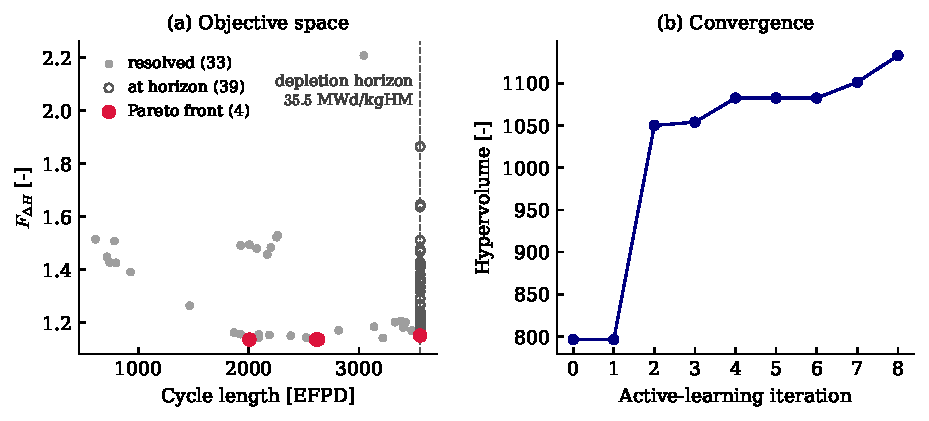
\includegraphics[width=\textwidth]{images/th_c1_front.pdf}
  \caption[Campaign 1 from the recovered checkpoint]{Campaign 1 from the recovered checkpoint. (a)~Objective space. (b)~Hypervolume history over the nine recorded active-learning iterations, reference point $(-1787.5,\ 1.785)$.}
  \label{fig:c1-front}
\end{figure}

\subsection{Campaign 2: the horizon test and the estimator}
\label{sec:res-c2}

Campaign 2 corrected both defects of the shakedown deliberately and
added the tabulated $k$-target calibration, the adaptive depletion
schedule and the geometry constraint. It raised the depletion horizon
from 35.5 to 100\,MWd/kgHM, a factor of 2.8, and completed 84
evaluations in two blocks, a 54-evaluation design of experiments and a
checkpoint-resumed block of five infill iterations of six points.

The horizon increase functioned as an unplanned experiment. The
censored fraction moved from 54.2\% to 59.5\%, essentially unchanged,
and all 50 censored designs again report the identical converted
horizon of 10016.7\,EFPD. The closest resolved design terminated at
10008.3\,EFPD, within 0.08\% of the cap. Tripling the horizon therefore
did not resolve the objective. The degeneracy is generated by the
design space itself, in which enrichments approaching the LEU cap
combined with thick reflectors carry a reactivity inventory that
sustains criticality far beyond any operationally meaningful cycle.
The remedy adopted from Campaign 3 onward is the physically grounded
discharge limit of Section~\ref{sec:meth-atf}, enforced inside the
depletion loop, which converts the arbitrary horizon into a
design-basis bound and eliminates censoring by construction.

The entries at the horizon carry no design meaning. The reported
refuelling interval of five years corresponds to 913 to 1461
EFPD at capacity factors between 0.5 and 0.8
(Section~\ref{sec:res-c8-mission}), so a cycle length of several
thousand days exceeds the mission by a factor of five to ten. Such a
design carries at beginning of life a reactivity inventory that the
controllability screen of Section~\ref{sec:meth-ctrl} later shows to
be beyond the regulating banks, and the horizon values measure that
inventory rather than describe a credible core.

Campaign 2 also exposed the estimator pathology
(Table~\ref{tab:c2-summary}). The stored single-seed peaking values
carried a bias larger than the front spread they ranked, and resolving
the candidates at high fidelity inverted the ranking. The stored fourth
became the true first, the apparent winner fell to seventh, and the
pair separated at $|t| = 12.8$. The statistical treatment that this
finding forced, per-design seeding, the fidelity ladder and two-stage
subset selection, is specified in Sections~\ref{sec:meth-fidelity}
and~\ref{sec:meth-stats}.

\begin{table}[htbp]
  \centering
  \caption{Campaign 2 in five numbers.}
  \label{tab:c2-summary}
  \begin{tabular}{lc}
    \toprule
    Uncapped front span, EFPD / $F_{\Delta H}$ & 17.7\% / 5.1\% \\
    Seed-to-seed s.d.\ of $F_{\Delta H}$ (stored fidelity) & up to 0.018 \\
    Bias of the stored values vs 256k reference & $-0.07$ \\
    Ranking outcome after resolution & inverted (4th $\to$ 1st) \\
    Corrected 75\,MWd/kgHM front & 2 designs (trade-off restored) \\
    \bottomrule
  \end{tabular}
\end{table}

The seed-to-seed standard deviation in Table~\ref{tab:c2-summary} comes
from a replication of the three lowest-peaking front designs at the
stored fidelity of $4\,000\times60$, with five seeds each. The
per-design values are 0.018, 0.007 and 0.018, and the pooled value is
$0.015\pm0.003$.

\subsection{Hypervolume comparability across campaigns}
\label{sec:res-hv-comparability}

The recovered archives fix the hypervolume reference points of the
early campaigns at $(-1787.5,\ 1.785)$ for Campaign 1 and
$(-5063.4,\ 1.976)$ for Campaign 2, in signed objective space. The
reference points differ on both axes, and the objective definition
itself changed when the discharge limit entered the cycle-length
objective. Hypervolume magnitudes are therefore not comparable across
campaigns, and none are compared in this work. Each history is read
only for its internal convergence shape, consistent with the reset
policy of Section~\ref{sec:meth-atf}. Any future cross-campaign figure
must first recompute all histories against a single reference point
taken as the componentwise worst value over the union of the archives,
a pure post-processing step on the committed checkpoints.

\openpoint{Pin the exact Campaign 1 code state (one of the four
commits of 10 July 2026) and the step list of the default depletion
schedule by inspecting the evaluator at that commit. Verify the
Campaign 2 feasible count of 44 directly from the recovered checkpoint
before the viva.}

% ============================ end of drop-in ==========================

\section{Campaign 3: design of experiments and feasibility envelope}
\label{sec:res-c3doe}

Campaign 3 (72 evaluations at $16\,000\times120$, per-design seeds, ATF
limit in-loop) opens with a 36-point Latin hypercube: 11 feasible
(31\%), with the upper reactivity bound responsible for 21 of 25
rejections. Regression over the archive gives the feasibility envelope
($R^2 = 0.92$--$0.94$, stable from $n=36$ to $n=72$):
\begin{equation}
  k_\mathrm{BOL} \;=\; 0.894 \;+\; 0.215\,\ln e_\mathrm{vw}
  \;-\; 0.0066\,\mathrm{gd},
  \qquad
  e_\mathrm{vw} = 0.72\,e_\mathrm{out} + 0.28\,e_\mathrm{in}.
  \label{eq:envelope}
\end{equation}

Three readings of Eq.~\eqref{eq:envelope} organise the design space.
Volume-weighted enrichment governs: the 72/28 zone split makes
$e_\mathrm{out}$ dominant by construction. Gadolinium at the fixed
twelve-pin pattern buys only $\Delta k \approx 0.05$--$0.06$ over its
full range, which is 2.7\,wt\% of enrichment headroom, against layouts
of up to 40 poisoned pins per assembly studied for soluble-boron-free
cores~\cite{rr_smr_atf_2025,ismr_sbf_2024}. And pitch emerges as the
second feasibility lever (logistic coefficient $+1.67$ at $n=72$,
behind only $e_\mathrm{out}$): over-moderation reaches criticality at
low enrichment. The envelope figure generated from the archive
(\texttt{figs/envelope\_b2}) belongs here.

\section{Campaign 3: convergence and the resolved front}
\label{sec:res-c3front}

Figure~\ref{fig:hv} shows the hypervolume of Campaign 3. Block 1 delivers
the gains, and Block 2 returns three consecutive exact zeros, so the
stopping rule is met with margin.

\begin{figure}[htbp]
  \centering
  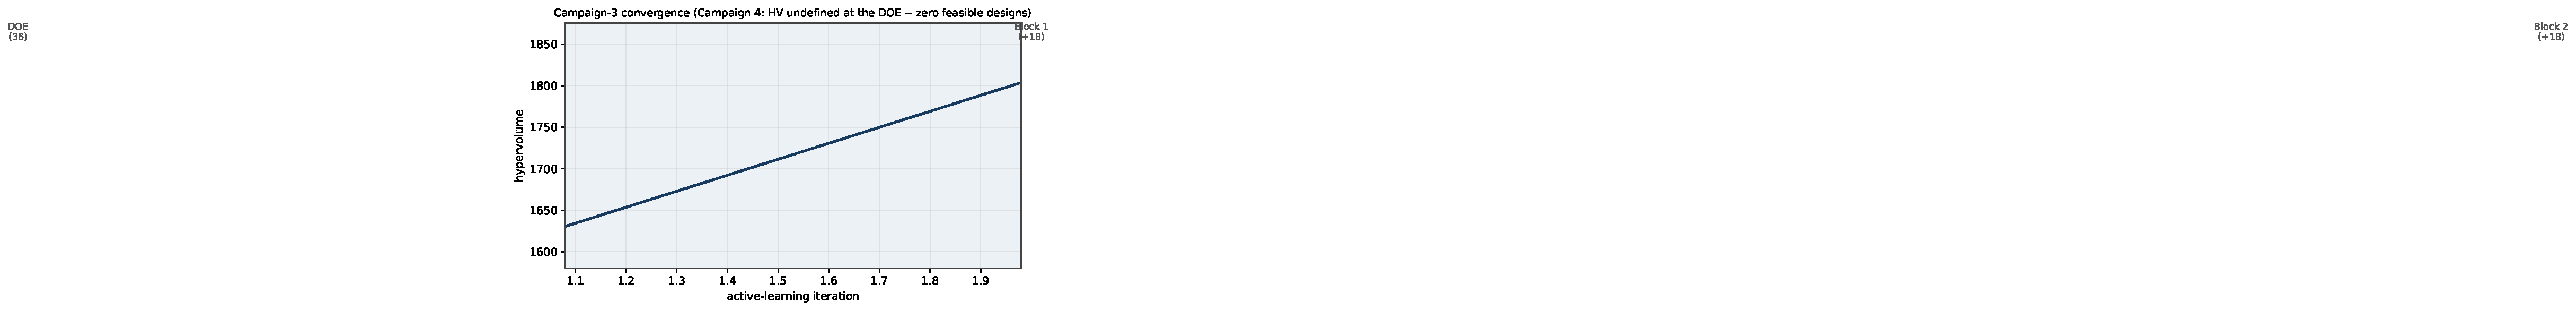
\includegraphics[width=0.86\linewidth]{images/th_hv_history}
  \caption{Campaign 3 hypervolume.}
  \label{fig:hv}
\end{figure}

Block behaviour carries information beyond the trajectory
(Fig.~\ref{fig:hv}): Block-1 infill was \textbf{18/18 feasible} against
the DOE's 31\%, because the surrogate had learned the reactivity
boundary, and only 6/18 at the burnup cap, walking into the below-cap region where
a trade-off exists. Block 2 (7/18 feasible, 18/18 at the cap) probed
the constraint boundary of an already-stable front: the signature of
convergence seen from inside.

High-fidelity resolution ($256\,000\times8$ seeds,
Fig.~\ref{fig:plateau}) then reshapes the stored front
(Table~\ref{tab:c3-resolved}). The shifts are design-dependent, from
$-0.003$ to $-0.020$, and the four plateau members are pairwise
unresolved. The design-dependent bias re-orders the set a second time,
after Campaign 2.

\begin{table}[htbp]
  \centering
  \caption{Campaign 3 finalists after high-fidelity resolution.}
  \label{tab:c3-resolved}
  \begin{tabular}{lcccc}
    \toprule
    & stored & measured (95\% CI) & shift & EFPD \\
    \midrule
    cand2 & 1.1336 & $1.1212\pm0.0021$ & $-0.0124$ & 5\,239 \\
    cand0 & 1.1266 & $1.1213\pm0.0019$ & $-0.0053$ & 5\,180 \\
    cand5 & 1.1445 & $1.1241\pm0.0010$ & $-0.0204$ & 5\,902 \\
    cand1 & 1.1270 & $1.1244\pm0.0010$ & $-0.0026$ & 2\,904 \\
    \midrule
    cand6 & 1.1483 & $1.1291\pm0.0023$ & $-0.0192$ & 5\,358 \\
    cand7 (capped) & 1.1522 & $1.1319\pm0.0038^{\dagger}$ & --- & 7\,513 \\
    cand3 (capped) & 1.1397 & $1.1381\pm0.0037^{\dagger}$ & --- & 7\,513 \\
    \bottomrule
    \multicolumn{5}{l}{\footnotesize $^{\dagger}$64k measurement,
    bias-adjusted to 256k; cand7 beats cand3 at $|t|=3.38$ (measured).}
  \end{tabular}
\end{table}

\begin{figure}[htbp]
  \centering
  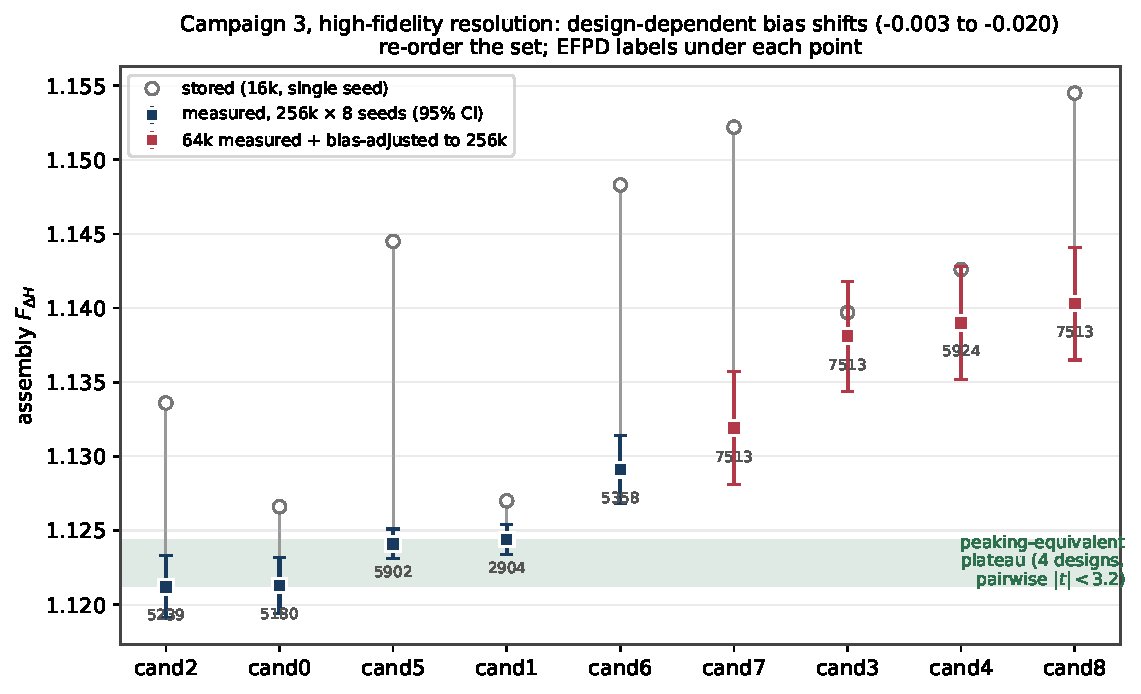
\includegraphics[width=0.9\linewidth]{images/th_c3_plateau}
  \caption{Stored versus resolved peaking of the Campaign 3 finalists.}
  \label{fig:plateau}
\end{figure}

The assembly-level result is therefore \textbf{a plateau, not a
winner}: four designs statistically identical in $F_{\Delta H}$
(1.1212--1.1244) spanning 2\,904--5\,902\,EFPD, plus the capped
strategy at 7\,513\,EFPD led by cand7, which is itself not separated
from the plateau once bias-adjusted ($|t|=2.6$). Two engineering strategies
emerge: a thick-reflector, high-enrichment capped design pressed
against the vessel ($g_\mathrm{geom}=-0.4$\,cm), and an over-moderated
cluster (pitch 1.41, enrichment $\sim$5.3\,wt\%, thin reflector).
Both are shaped by the same scarce resource, the 90\,cm vessel radius
(Eq.~\ref{eq:renv}).
%% AUTHOR: 2-3 sentences of physics on the two strategies (reflector
%% leakage vs over-moderation; MTC risk of the wide-pitch cluster).

\section{Core-level validation: the proxy gap}
\label{sec:res-corevalidation}

Rebuilding the finalists as full cores (BOL, 8 seeds) measures what the
reflective assembly cannot see (Table~\ref{tab:core-finalists}).

\begin{table}[htbp]
  \centering
  \caption{Campaign 3 finalists at core level ($100\,000\times$ up to 230 batches, 8 seeds).}
  \label{tab:core-finalists}
  \begin{tabular}{lcccc}
    \toprule
    & $F_{\Delta H}^\mathrm{asm}$ & $F_{\Delta H}^\mathrm{core}$
      (95\% CI) & ratio & EFPD \\
    \midrule
    idx46 (cand3) & 1.1397 & $2.013\pm0.018$ & 1.77 & 7\,513 \\
    idx45 (cand7) & 1.1522 & $2.020\pm0.019$ & 1.75 & 7\,513 \\
    idx53 (cand5) & 1.1445 & $2.114\pm0.018$ & 1.85 & 5\,902 \\
    \bottomrule
  \end{tabular}
\end{table}

Three facts. The proxy gap is a factor \textbf{1.75--1.91},
anti-correlated with reflector thickness ($r=-0.96$ over the six
finalists): thin reflectors leak, depress the periphery, and drive
core-wide peaking, an effect invisible to an infinite lattice. The ranking
\emph{inverts}: the assembly-best design is core-worst, and the capped
pair (idx46/idx45, tied at $|t|=0.54$) beats the plateau at
$|t|\approx7$--$8$, collapsing the front to the capped strategy. And the
peaking constraint, inactive everywhere at assembly level, is now
\textbf{violated by every design}: the best sits at
$2.013\pm0.018$ against the 2.0 limit.

Rescoring the \emph{entire} feasible archive (36 designs,
Fig.~\ref{fig:asmcore}) generalises the finding. The proxy is globally
informative, with $\rho=+0.890$, yet scrambles the ordering exactly where
the optimiser operates. Table~\ref{tab:proxy-numbers} gives the proxy in
numbers and the designs it mis-ranked, with rank positions taken among
the 36 feasible Campaign 3 designs.

\begin{figure}[htbp]
  \centering
  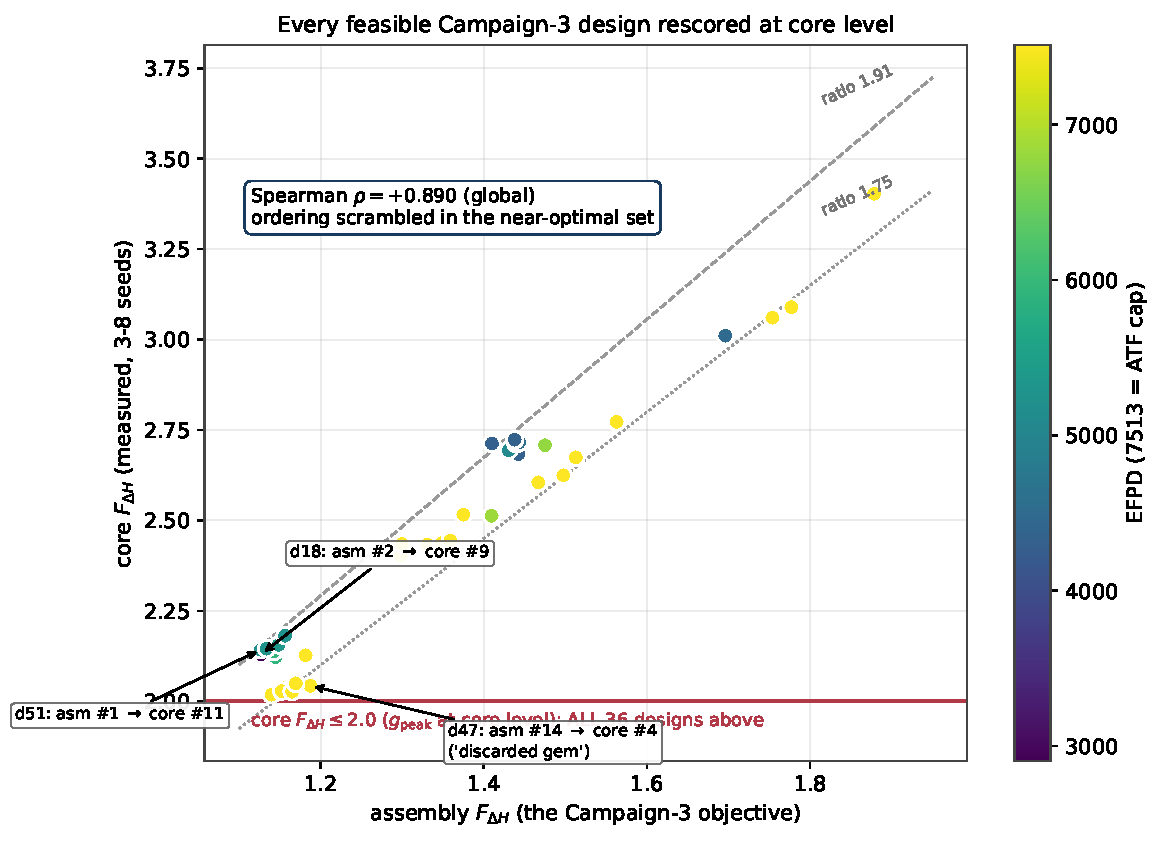
\includegraphics[width=0.9\linewidth]{images/th_asm_vs_core}
  \caption{Every feasible Campaign 3 design rescored at core level.}
  \label{fig:asmcore}
\end{figure}

\begin{table}[htbp]
  \centering
  \small
  \caption{The proxy in numbers, and the designs it mis-ranked.}
  \label{tab:proxy-numbers}
  \begin{tabularx}{\textwidth}{@{}>{\raggedright\arraybackslash}p{0.48\textwidth}>{\raggedright\arraybackslash}X@{}}
    \toprule
    Quantity & Value \\
    \midrule
    Spearman $\rho$, assembly versus core, $n=36$
      & $+0.890$ \\
    Assembly ranks 1 / 2 / 3, re-evaluated at core level
      & 11 / 9 / 12 \\
    Largest rank gains, the discarded gems
      & d47: \#14 $\to$ \#4 \newline
        d43: \#9 $\to$ \#2 \newline
        d42: \#11 $\to$ \#5 \\
    Core-level Pareto front
      & A single design, d46, violating $F_{\Delta H}\le 2.0$ \\
    Designs meeting $F_{\Delta H}^\mathrm{core}\le 2.0$
      & 0 of 36 \\
    \bottomrule
  \end{tabularx}
\end{table}

The bridge model (Eq.~\ref{eq:bridge}) fitted on all 36 designs,
\begin{equation}
  \frac{F^\mathrm{core}}{F^\mathrm{asm}}
  = 1.400 \;-\; 0.0045\,t_\mathrm{refl} \;+\; 0.343\,p,
  \qquad R^2 = 0.746,
  \label{eq:bridge-fit}
\end{equation}
confirms reflector and pitch as the corrupting variables, and its
residual quarter is the argument for measuring rather than correcting.
The fit describes the uniform loading of Campaign~3 only. On the zoned
core that the evaluator builds from Campaign~6 the ratio is smaller and
no longer depends on the geometry, as
Section~\ref{sec:res-proxy-gap-zoned} reports.

Route-B closure on the finalists gives residuals of $-91$ to
$-429$\,pcm (most negative for thick reflectors), validating the
cycle-length proxy at the $\sim$2\% level, and the Shannon-entropy
diagnostic of the core solves identified one case converging at batch 94 against a 40-batch
cutoff, which is the reason the production core solves carry 60 to 120
inactive batches.

\textbf{The methodological statement of the thesis follows:} a
surrogate-assisted optimisation on a reduced-order proxy must validate
the proxy's \emph{rank fidelity} near the optimum, not merely its
statistical convergence, because correlation weakens exactly where the
optimiser converges, and it did so here twice (estimator bias in
Campaign 2, geometric proxy in Campaign 3).

\section{Campaign 4: the core-level objective}
\label{sec:res-c4}

Campaign 4 moves $F_{\Delta H}$ and $g_\mathrm{peak}$ to core level at
$\approx3\%$ evaluation cost (Eq.~\ref{eq:corecost}) and is complete:
a 36-point DOE plus three infill iterations of six evaluations each,
54 designs in total, \textbf{zero feasible}
(Table~\ref{tab:c4-doe}, Fig.~\ref{fig:c4traj}). With an empty feasible set
the hypervolume is undefined and is reported as zero, so convergence is
judged on the reduction of the constraint violation.

\begin{table}[htbp]
  \centering
  \caption{Campaign 4 design of experiments against that of Campaign 3, with the same limits and design space.}
  \label{tab:c4-doe}
  \begin{tabular}{lcc}
    \toprule
    & C3 DOE (assembly $g_\mathrm{peak}$) & C4 DOE (core
      $g_\mathrm{peak}$) \\
    \midrule
    feasible                     & 11 / 36 & \textbf{0 / 36} \\
    $g_\mathrm{peak}$ violations & 4       & \textbf{35} \\
    $g_{k\max}$ violations       & 21      & 24 \\
    best $F_{\Delta H}$ (its level) & 1.127 & 1.9215 \\
    \bottomrule
  \end{tabular}
\end{table}

\begin{figure}[htbp]
  \centering
  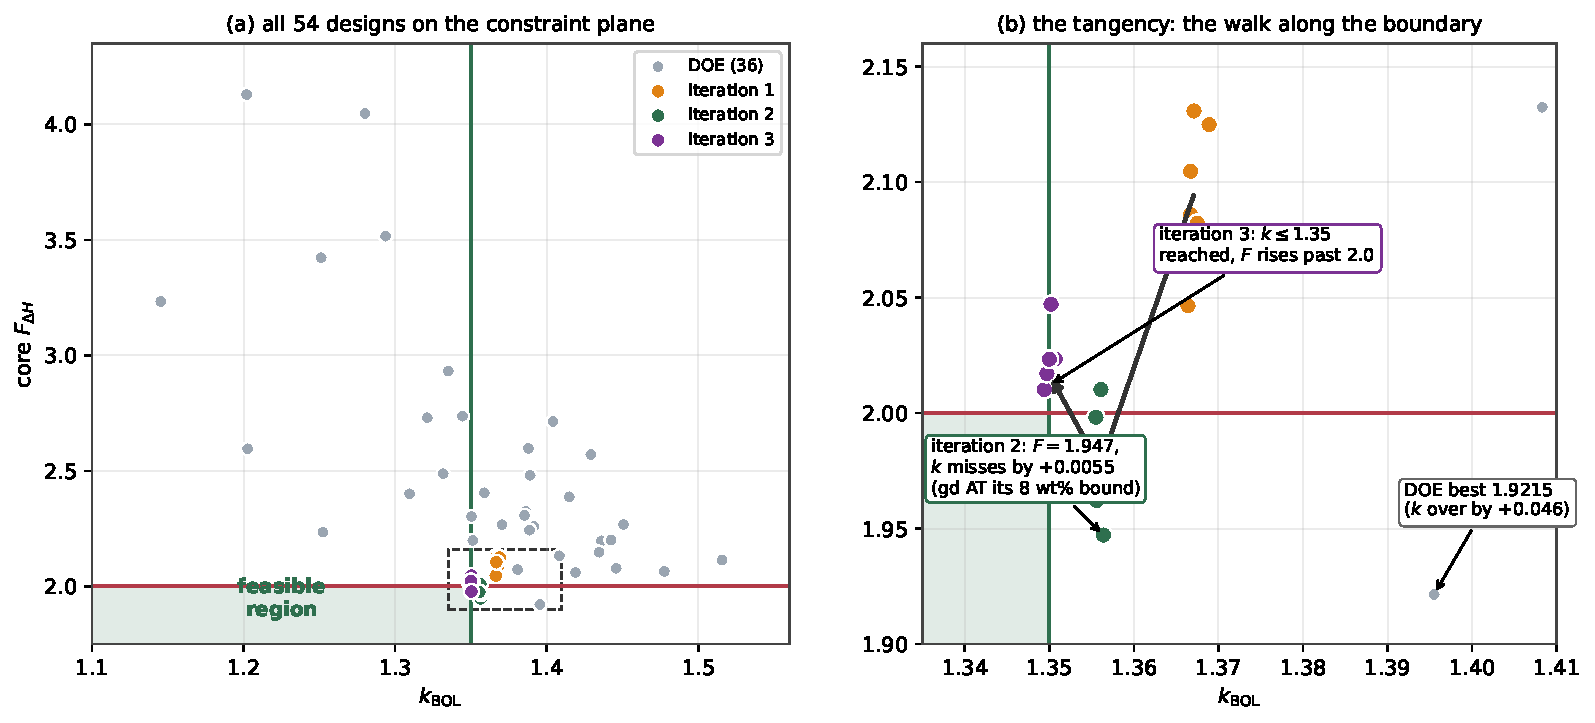
\includegraphics[width=\linewidth]{images/c4_trajectory}
  \caption[Campaign 4 on the constraint plane]{Campaign 4 on the constraint plane. (a)~All 54 designs. (b)~The three-iteration walk along the boundary.}
  \label{fig:c4traj}
\end{figure}

\subsection{Infill trajectory and the tangency of the feasible region}
\label{sec:res-c4-trajectory}

The infill ran under constraint-violation ranking throughout, since no
design was ever feasible. Its trajectory
(Table~\ref{tab:c4-trajectory}) is the campaign's central measurement. The
total violation reaches its minimum at iteration 2 and rises again at
iteration 3, when $k_\mathrm{BOL}\leq1.35$ is finally satisfied.

\begin{table}[htbp]
  \centering
  \caption{Campaign 4 infill iterations: ranges over the six designs of each iteration.}
  \label{tab:c4-trajectory}
  \begin{tabular}{ccccc}
    \toprule
    iteration & $k_\mathrm{BOL}$ & core $F_{\Delta H}$ &
      mean total violation \\
    \midrule
    DOE  & 1.145 -- 1.516 & 1.921 -- 4.129 & 0.084 \\
    1    & 1.3664 -- 1.3689 & 2.046 -- 2.131 & 0.1131 \\
    2    & 1.3555 -- 1.3567 & \textbf{1.947} -- 2.010 & \textbf{0.0077} \\
    3    & \textbf{1.3494} -- 1.3507 & 1.977 -- 2.047 & 0.0204 \\
    \bottomrule
  \end{tabular}
\end{table}

Three facts define the outcome. The optimiser collapsed the reactivity
spread by a factor of 200 (DOE $k_\mathrm{BOL}$ standard deviation
0.081; iteration-1 spread 0.0025) and then walked $k_\mathrm{BOL}$
down through the limit across iterations. Iteration 2 achieved
designs feasible on peaking ($F_{\Delta H}=1.947$--$2.010$) missing
only the reactivity limit, by $+0.0055$ to $+0.0067$. Iteration 3
satisfied the reactivity limit ($k_\mathrm{BOL}=1.3494$--$1.3507$) and
lost peaking feasibility in exchange.

The two constraints are therefore \textbf{tangent, not overlapping},
within this five-variable space: each is satisfiable alone, their
intersection was never reached, and the converged residual gap is
$\Delta k \approx 0.006$ measured at the point of closest approach.

\subsection{Exhaustion of the design space at a vertex}
\label{sec:res-c4-vertex}

Figure~\ref{fig:c4parallel} shows the Campaign 4 designs in parallel
coordinates by phase, with the design of experiments in grey filling the
box.

\begin{figure}[htbp]
  \centering
  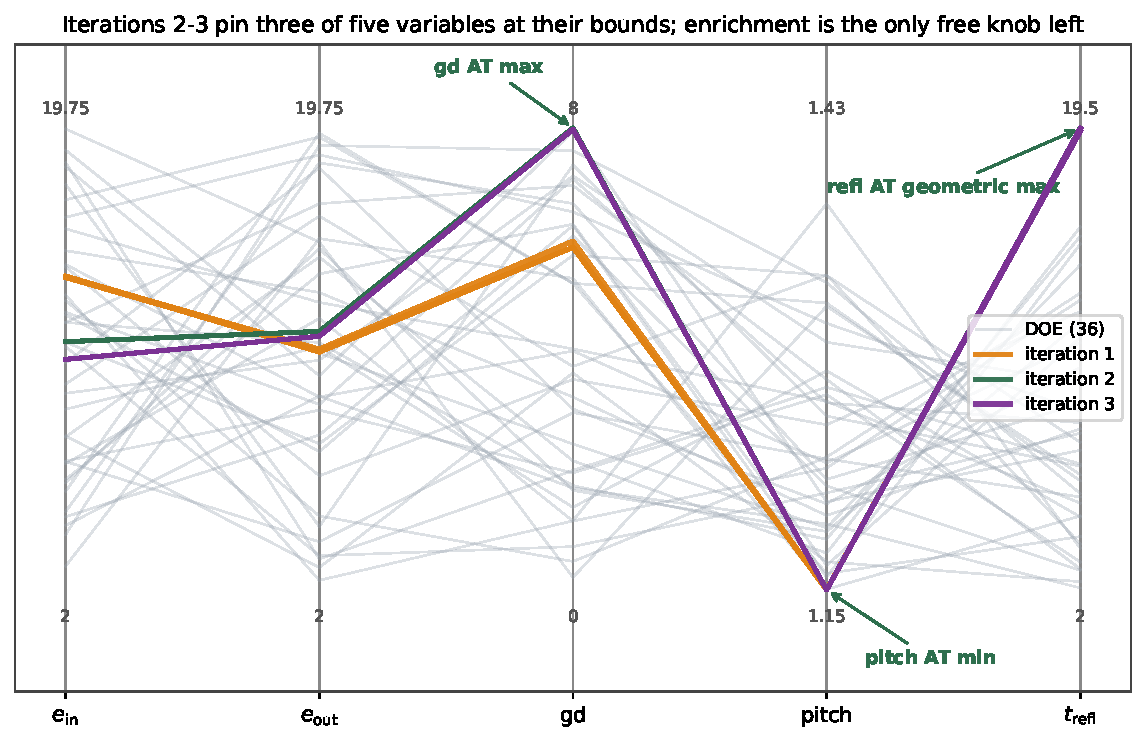
\includegraphics[width=0.92\linewidth]{images/c4_parallel}
  \caption{Campaign 4 design variables in parallel coordinates by phase.}
  \label{fig:c4parallel}
\end{figure}

Every iteration-2 and iteration-3 design pins \textbf{three of the five
variables at their bounds} (Fig.~\ref{fig:c4parallel}): gadolinium
concentration at 8.0\,wt\% (to four decimals), pitch at 1.150\,cm, and
reflector thickness at the vessel-budget ceiling
(Eq.~\ref{eq:renv}). The sole remaining degree of freedom, enrichment,
is what the optimiser walks: $e_\mathrm{vw}=11.82$\,wt\% at iteration 2
to $11.50$\,wt\% at iteration 3. That slide \emph{is} the
$k_\mathrm{BOL}$ descent of Table~\ref{tab:c4-trajectory}.

The constrained optimum of Campaign 4 therefore sits at a vertex of the
design box, and the optimiser is, in effect, requesting more absorber
than the concentration bound permits. The identified resolution,
absorber \emph{inventory} as a variable, follows in
Section~\ref{sec:res-campaign5}.

The pitch bound reached at iterations 2 and 3 carries the geometric
caveat established later in this work. Below \SI{1.2242}{cm} the
lattice clips the guide-tube wall silently, so the eigenvalues and the
peaking values of the \SI{1.150}{cm} designs of this campaign are
biased by an unquantified amount
(Section~\ref{sec:res-c7-limits}).

\subsection{Variable influence and the champion designs}
\label{sec:res-c4-champions}

Figure~\ref{fig:c4influence} plots each design variable against the core
peaking factor over all 54 designs. Volume-weighted enrichment dominates,
with $r=-0.59$, and $-0.63$ for $e_\mathrm{out}$ alone. Gadolinium is
peaking-neutral at $r=-0.16$, because it buys reactivity without
flattening the power, which is why the conflict is structural.

Figure~\ref{fig:c4objectives} shows the objective plane. With 46 of 54
designs at the 75\,MWd/kgHM cap the trade-off degenerates. The
unconstrained non-dominated set is a single infeasible capped design, and
the campaign is effectively a single-objective constrained minimisation
of core peaking. Table~\ref{tab:c4-champions} lists the champion designs.

\begin{figure}[htbp]
  \centering
  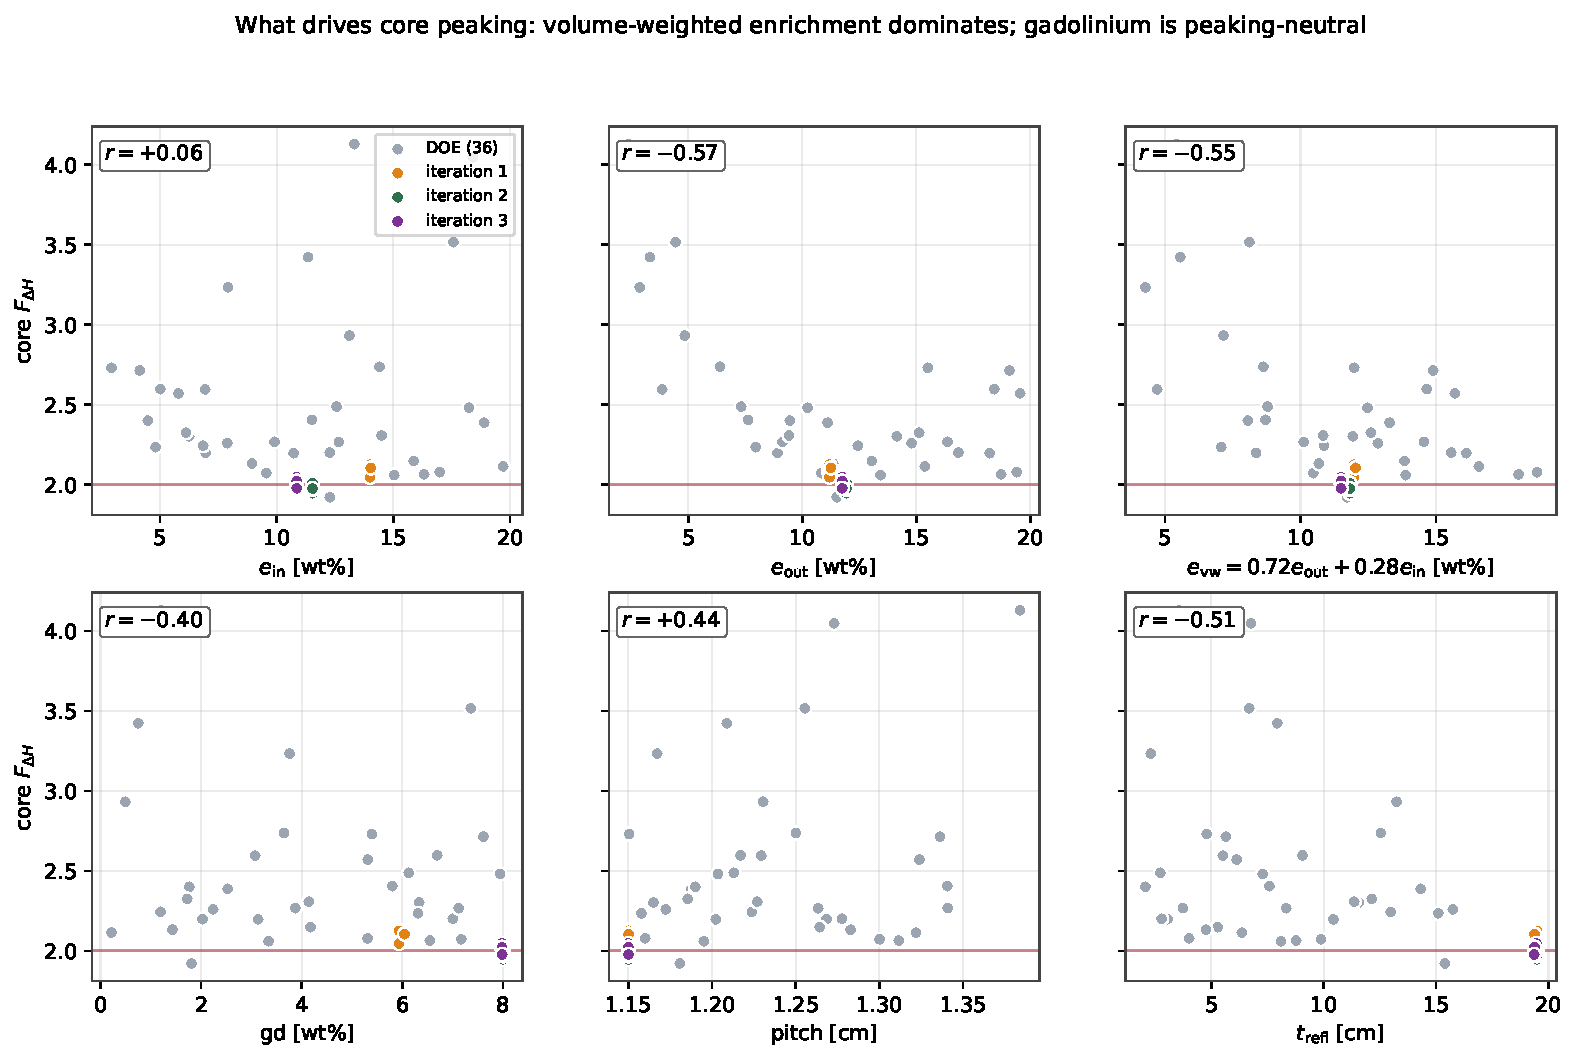
\includegraphics[width=\linewidth]{images/c4_influence}
  \caption{Campaign 4 design variables against core $F_{\Delta H}$, all 54 designs.}
  \label{fig:c4influence}
\end{figure}

\begin{figure}[htbp]
  \centering
  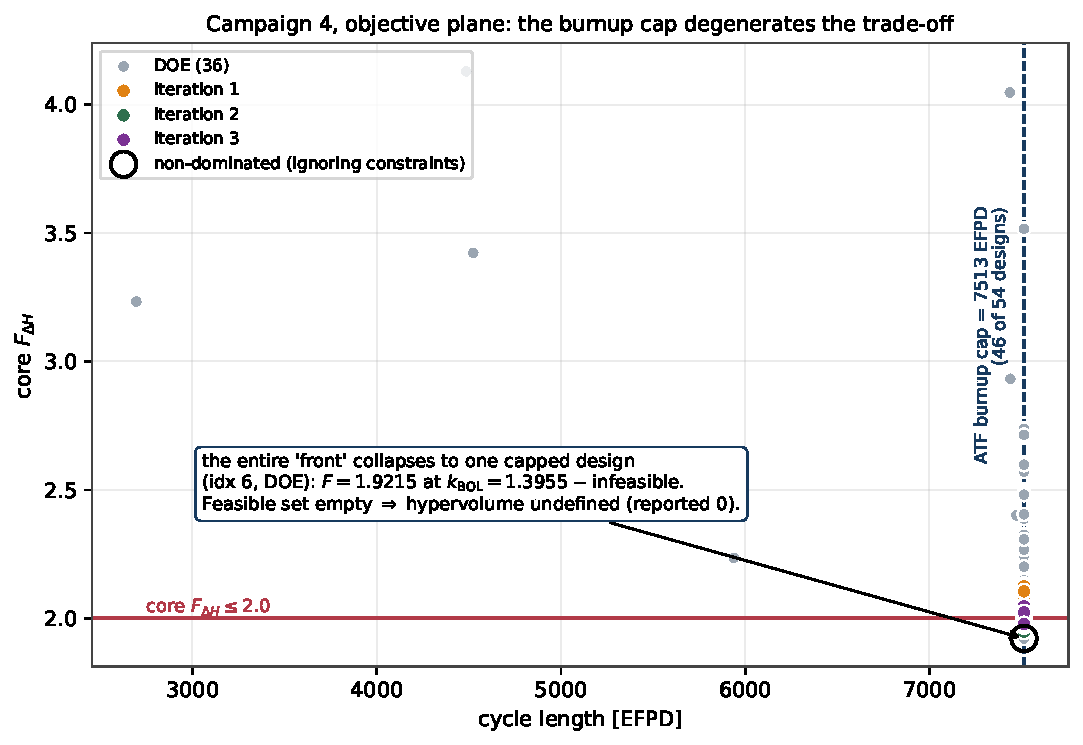
\includegraphics[width=0.9\linewidth]{images/c4_objectives}
  \caption{Campaign 4 objective plane.}
  \label{fig:c4objectives}
\end{figure}

\begin{table}[htbp]
  \centering
  \small
  \caption{The champion designs of Campaign~4. Bold marks a value
  sitting at a design-space bound.}
  \label{tab:c4-champions}
  \begin{tabularx}{\textwidth}{@{}>{\raggedright\arraybackslash}p{0.26\textwidth}*{3}{>{\centering\arraybackslash}X}@{}}
    \toprule
    Quantity & idx 6, DOE & idx 44, iteration 2 & Iteration 3, typical \\
    \midrule
    $e_\mathrm{in}$ / $e_\mathrm{out}$ [wt\%]
      & 12.28 / 11.50 & 11.54 / 11.93 & $e_\mathrm{vw} = 11.50$ \\
    Gd$_2$O$_3$ content [wt\%]
      & 1.81 & \textbf{8.00} & 7.98 \\
    Pitch [cm]
      & 1.181 & \textbf{1.150} & \textbf{1.150} \\
    $t_\mathrm{refl}$ [cm]
      & 15.39 & \textbf{19.49} & 19.35--19.48 \\
    Core $F_{\Delta H}$ [--]
      & \textbf{1.9215} & 1.9472 & 1.977--2.047 \\
    $k_\mathrm{BOL}$ [--]
      & 1.3955 & 1.3564 & 1.3494--1.3507 \\
    Status
      & Peaking met, $k_\mathrm{BOL}$ high by 0.046
      & Closest approach, $k_\mathrm{BOL}$ high by 0.0055
      & $k_\mathrm{BOL}$ met, peaking exceeded \\
    \bottomrule
  \end{tabularx}
\end{table}

Design idx 44 deserves one further remark: its reflector sits at
19.4914\,cm at pitch 1.150\,cm, exactly the corrected geometric
ceiling. The optimiser found the vessel-budget corner twice: once
illegally, through a 0.02\,cm inconsistency between the analytic
constraint and the geometry builder (crashing the first infill
attempt; the fix made the builder's fuel-envelope pad part of
$g_\mathrm{geom}$), and once legally, after the fix. Both episodes,
together with a mid-loop failure of the optimiser on an empty feasible
set (repaired by a least-infeasible infill fallback and per-iteration
checkpointing), are recorded in the methodology diagnostics: an
optimiser pressing on constraint boundaries is an adversarial
verification tool, and it found two real defects this way.
%% AUTHOR: 1-2 sentences of physics on WHY high enrichment flattens the
%% core radial profile (periphery-to-centre gradient, migration).

\section{Campaign 5: the absorber inventory as a design variable}
\label{sec:res-campaign5}

Campaign 4's converged residual is small and precisely located:
$\Delta k \approx 0.006$ at the iteration-2 champion, with the
concentration route closed by its own bound. Scaling the fitted 12-pin
authority (0.0525 in $\Delta k$ at 8\,wt\%) by inventory,
\begin{equation}
  \Delta k_\mathrm{pins}(n) \;=\; 0.0525\,\frac{n-12}{12}
  \;\;\Rightarrow\;\;
  n \;\approx\; 13.5 ,
  \label{eq:pins-needed}
\end{equation}

so \textbf{approximately two additional gadolinia pins} were predicted to
close the gap, a far smaller departure from the twelve-pin heritage pattern
than the DOE-based estimate of approximately 23 pins suggested before the
infill located the true point of closest approach. Campaign 5 was designed
to test that prediction by admitting the pin count as a search variable
rather than fixing it. Table~\ref{tab:c5} lists the changes relative to
Campaign 4, one of them structural to the search space, and the
disposition of each at the close of the campaign.

\begin{table}[htbp]
  \centering
  \small
  \caption[Campaign 5 relative to Campaign 4]{Campaign 5 relative to Campaign 4: changes and their disposition at the close of the campaign.}
  \label{tab:c5}
  \begin{tabularx}{\textwidth}{@{}>{\raggedright\arraybackslash}p{0.24\textwidth}>{\raggedright\arraybackslash}X>{\raggedright\arraybackslash}p{0.24\textwidth}@{}}
    \toprule
    Change & Rationale & Disposition \\
    \midrule
    Gd pin count as sixth design variable, 12 to 40 rods in
    octant-symmetric patterns
      & The optimiser exhausted the concentration bound
        (Fig.~\ref{fig:c4parallel}). Inventory scales absorber authority
        without the self-shielding penalty and is the primary lever
        reported in the literature at a fixed weight fraction of
        approximately 8\,wt\%~\cite{rr_smr_atf_2025}
      & Implemented. Minimum total constraint violation fell from 0.0077
        to 0.0012 (Fig.~\ref{fig:c5traj}) \\
    Single-design pin-count test on idx 44
      & Re-evaluation at 14, 16 and 20 rods to decide within hours
        whether the tangency opens
      & Executed. Feasibility reached at 14 rods,
        $k_\mathrm{BOL}=1.3456$, at a measured authority of
        approximately \SI{500}{pcm} per rod (Fig.~\ref{fig:c5pins}) \\
    Constraint normalisation by individual limits
      & The Campaign 1 to 4 violation sum added quantities in
        $\Delta k$, peaking factor, weight percent and centimetres
        without weighting
      & Implemented in Campaign 5 \\
    $g_{k\max}$ moved to core $k_\mathrm{eff}$
      & Excess reactivity is a core quantity, and
        $k_\mathrm{eff}^\mathrm{core}$ is already recorded per
        evaluation at no additional cost
      & Not applied during the search. Applied retrospectively to both
        archives in Section~\ref{sec:res-c5-kbasis}, where it admits
        exactly the designs the assembly screen admits at 1.40 \\
    Soluble-boron decision
      & Civil soluble-boron-free practice~\cite{ismr_sbf_2024,acp100_physor2020}
        motivates a boron-free basis. Removing the boron raises
        $k_\mathrm{BOL}$ by approximately 0.08 to 0.10,
        which tightens the problem rather than relaxing it
      & Closed. The \SI{1000}{ppm} benchmark-traceable basis of
        Section~\ref{sec:meth-boron} is retained for all campaigns, and
        the boron-free case is recorded as future work \\
    Review of the 1.35 bound
      & The limit proxies controllable excess reactivity without a rod
        model. At 1.40 both champions of
        Table~\ref{tab:c4-champions} are already feasible
      & Resolved by the re-scoring of Section~\ref{sec:res-c5-kbasis},
        which shows that the basis change and the relaxation to 1.40
        select identical design sets, and traced in Campaign 7 to the
        measured all-bank controllability bound of 1.368
        (Section~\ref{sec:res-c7-worth}) \\
    \bottomrule
  \end{tabularx}
\end{table}

The single-design test settles the Campaign 4 prediction before the
campaign results are examined. Re-evaluating the Campaign 4 champion at
14, 16 and 20 gadolinia rods measures an inventory authority of
approximately \SI{500}{pcm} per rod, so the two-rod step from 12 to 14
removes \SI{1011}{pcm} against the required \SI{640}{pcm}. The design is
feasible on both screening constraints at 14 rods, which confirms the
prediction of Equation~\eqref{eq:pins-needed} within one rod. The core
peaking factor is unchanged across the four counts, remaining between
1.970 and 1.995, so the inventory buys reactivity control and no peaking
penalty, consistent with the variable-influence finding of
Section~\ref{sec:res-c4-champions}.

In Figure~\ref{fig:c5pins} the assembly eigenvalue, left, crosses the
screening limit between 12 and 14 rods, and a fit over the four counts
gives an authority of \SI{535}{pcm} per rod. The core radial peaking
factor, right, is statistically flat across the four counts. The error
bars are one standard error of the mean.

\begin{figure}[htbp]
  \centering
  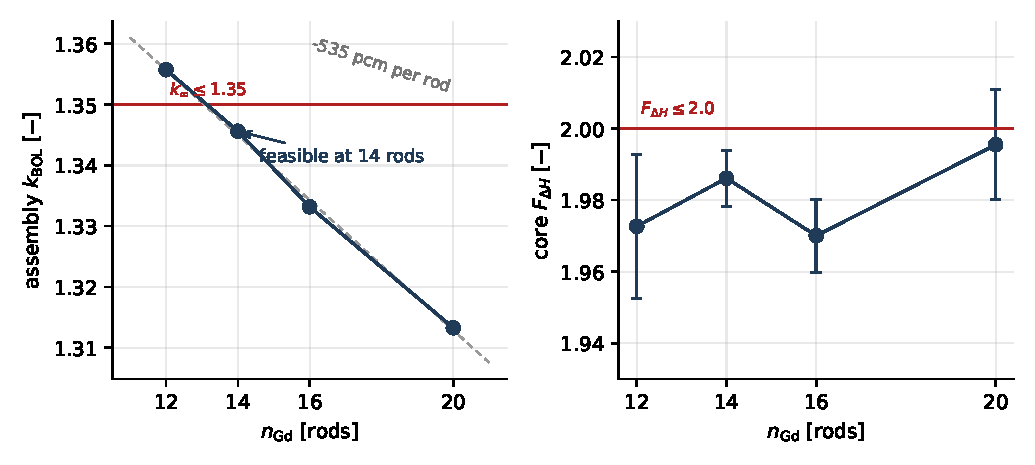
\includegraphics[width=0.95\linewidth]{images/c5_pin_worth}
  \caption[Pin-count test on the Campaign 4 champion]{Pin-count test on the Campaign 4 champion, archive index 44, at 12, 14, 16 and 20 gadolinia rods.}
  \label{fig:c5pins}
\end{figure}

\subsection{Search outcome under the as-run constraints}
\label{sec:res-c5-search}

Campaign 5 evaluated 60 designs, a 42-point Latin hypercube design of
experiments followed by three active-learning iterations of six real
evaluations each. The two blocks ran on consecutive days and the active
wall time was \SI{108.4}{\hour}, equal to 6934 core-hours, with the
complete cost decomposition recorded with the campaign checkpoint
(Appendix~\ref{app:code-architecture}).

The feasible set was empty at every recorded checkpoint. The hypervolume
history is identically zero at all four recorded points, the reference
point was never frozen because freezing requires a first feasible design,
and the empirical stopping rule of
Section~\ref{sec:res-hv-comparability} was therefore inoperative. The
campaign terminated on its iteration budget, not on convergence. Under an
empty feasible set the optimiser degrades to minimisation of the total
constraint violation
\begin{equation}
  V \;=\; \sum_{j} \max\!\left(0,\; \frac{g_j}{\lvert g_j^\mathrm{lim}
  \rvert}\right) ,
  \label{eq:violation-normalised}
\end{equation}

with the terms

\begin{itemize}
  \item $g_j$, the value of constraint $j$ in its native units,
  \item $g_j^\mathrm{lim}$, the limit of constraint $j$ in the same
        units, introduced as the per-constraint normalisation adopted in
        this campaign,
  \item $V$, the total normalised violation, dimensionless.
\end{itemize}

Figure~\ref{fig:c5traj} shows the resulting search trajectory, with the
running best as a step line. The design of experiments occupies indices
0 to 41, the three infill iterations follow in blocks of six, and the
three annotated designs are the champions discussed below. The best
design of experiments point reaches $V = 0.0264$ at archive index 17.
The first iteration does not improve on it, closing at $V = 0.0321$. The
second iteration reaches $V = 0.0074$ at index 49 and the third reaches
$V = 0.0012$ at index 54, the campaign champion. Relative to the best
Campaign 4 value of 0.0077, the sixth design variable moved the point of
closest approach by a factor of six.

\begin{figure}[htbp]
  \centering
  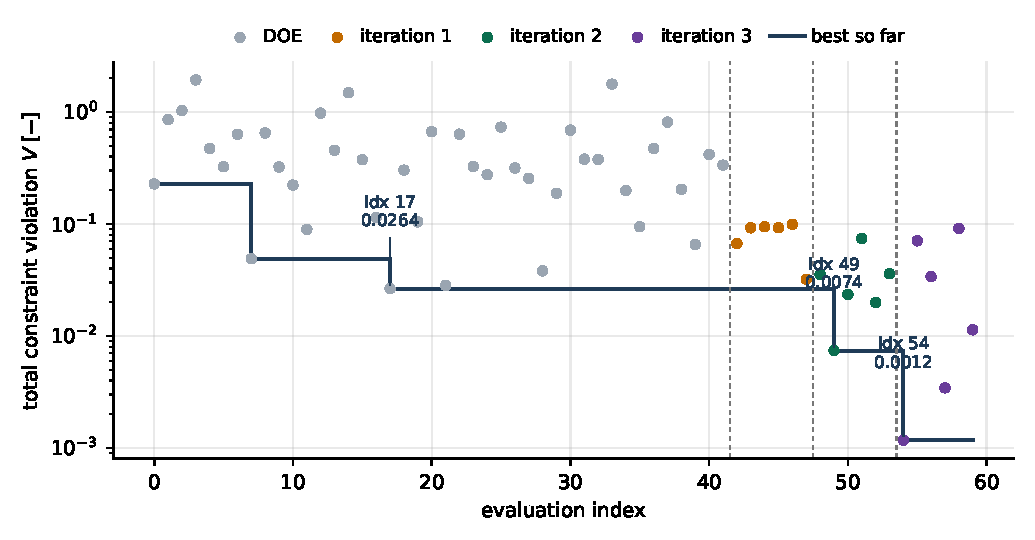
\includegraphics[width=0.95\linewidth]{images/c5_search_trajectory}
  \caption[Campaign 5 search trajectory]{Campaign 5 search trajectory: total normalised constraint violation per evaluation.}
  \label{fig:c5traj}
\end{figure}

All eighteen infill designs sit at the pitch lower bound of
\SI{1.150}{\centi\metre}, extending to six variables the vertex-seeking
behaviour documented for Campaign 4 in
Section~\ref{sec:res-c4-vertex}. Within that plane the three iterations
occupy three distinct regions of the design space
(Fig.~\ref{fig:c5lobes}, design of experiments points in grey):

\begin{enumerate}
  \item iteration 1 proposes 40 rods with gadolinia weight fractions of
        1.8 to 2.4\,wt\%, inner enrichment near the LEU cap at 18.1 to
        18.5\,wt\% and a thin reflector of 2.1 to \SI{5.8}{\centi\metre},
  \item iteration 2 proposes 12 rods with essentially zero gadolinia,
        both enrichments near 7.2\,wt\% and the reflector at its lower
        bound of \SI{2.0}{\centi\metre},
  \item iteration 3 proposes 40 rods with gadolinia weight fractions of
        1.4 to 1.9\,wt\%, inner enrichment near 13.2\,wt\% and the
        reflector at its geometric ceiling of 19.4 to
        \SI{19.5}{\centi\metre}.
\end{enumerate}

One geometric caveat applies to every design at this pitch. The
guide-tube outer radius of \SI{0.6121}{cm} exceeds the half-pitch below
\SI{1.2242}{cm}, and the lattice clips the tube wall at the cell
boundary silently, replacing up to \SI{27}{\percent} of the wall
cross-section by moderator at \SI{1.150}{cm}.

The defect was found while preparing Campaign 8, which fixes the pitch
at \SI{1.26}{cm} (Section~\ref{sec:meth-c8-space}). The vertex-seeking
result stands, because the optimiser was responding to the lattice it
was given. The absolute eigenvalues and peaking values of the
\SI{1.150}{cm} designs nevertheless carry an unquantified bias from the
extra moderator in the guide-tube ring.

\begin{figure}[htbp]
  \centering
  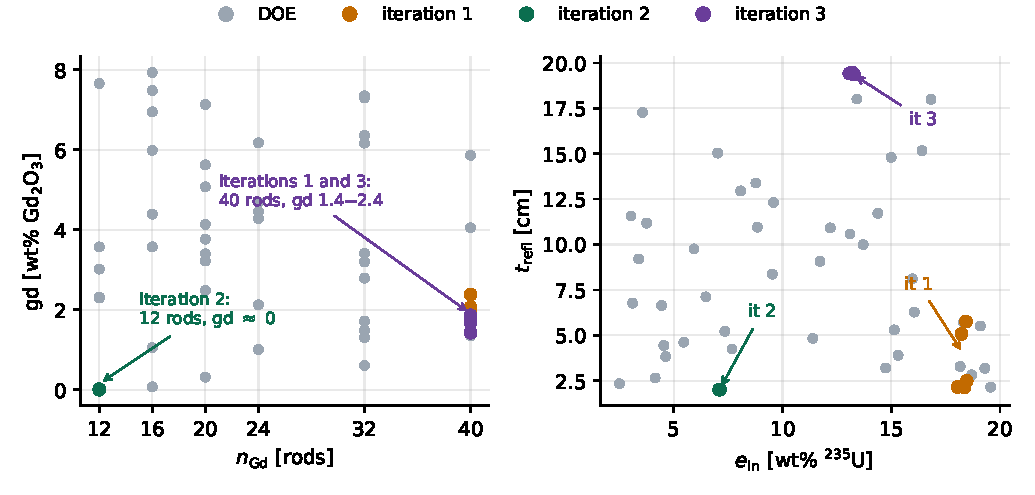
\includegraphics[width=0.95\linewidth]{images/c5_lobes}
  \caption[The two lobes of the Campaign 5 infill]{The two lobes of the Campaign 5 infill. Left, gadolinia weight fraction against rod count. Right, inner enrichment against reflector thickness.}
  \label{fig:c5lobes}
\end{figure}

The 40-rod iterations and the 12-rod iteration are two distinct routes
to the same reactivity screen. The first holds a large fissile inventory
in check with a large absorber inventory. The second carries so little
fissile inventory that almost no absorber is required.

%% AUTHOR: physics interpretation of the two lobes. Why the surrogate
%% found the zero-absorber lobe on its second iteration, what the two
%% routes imply for cycle length (the 12-rod lobe designs cross their
%% reactivity target near 3700 EFPD while the 40-rod lobe designs reach
%% the burnup ceiling), and which lobe is the better engineering basis.

\subsection{Corrected objectives}
\label{sec:res-c5-corrected}

Every cycle length recorded during the campaign is affected by the
depletion restart defect analysed in Section~\ref{sec:restart_defect}.
The salvage procedure of that section recovers the true burnups from the
archived histories without repeating any transport, and every
cycle-length statement in this subsection uses the corrected values. All
beginning-of-life quantities, in particular every peaking factor and
every eigenvalue in this chapter, are unaffected by construction.

The correction changes the population structure. The sixty evaluations
separate into three groups rather than the two reported by the evaluator:

\begin{enumerate}
  \item 18 designs crossed their reactivity target and possess a true,
        finite end of cycle,
  \item 39 designs reached the burnup ceiling, whose corrected physical
        value is \SI{43.0}{\mega\watt\day\per\kilo\gram} rather than the
        labelled \SI{75.0}{\mega\watt\day\per\kilo\gram}, so their
        corrected cycle lengths are lower bounds of \num{4307} Effective
        Full Power Days rather than the recorded \num{7513},
  \item 3 designs never reached criticality against their own
        end-of-cycle target and have no cycle at all. These were
        previously conflated with the ceiling group.
\end{enumerate}

The overstatement factor across the campaign is 1.68 on average, ranging
from 1.23 for early-terminating designs to 1.74 for designs that ran the
full schedule. The 413 discarded dead-step entries carry a mean
reactivity rise of \SI{785}{pcm}, in the range \SIrange{364}{1540}{pcm},
which identifies the chunk-locked period-two oscillation observed in the
recorded histories with the xenon signature of the defect rather than
with a property of the predictor integrator.

Figure~\ref{fig:c5objcorr} places the sixty Campaign 5 evaluations in the
corrected objective plane. Circles are designs that crossed their
reactivity target, plotted at the corrected end of cycle. Triangles are
designs censored at the burnup ceiling, plotted at the corrected ceiling
as lower bounds, and the three never-critical designs have no cycle and
are omitted. The collapse onto the ceiling line is the censoring
distortion of Section~\ref{sec:res-c2}, reproduced at the corrected
ceiling.

\begin{figure}[htbp]
  \centering
  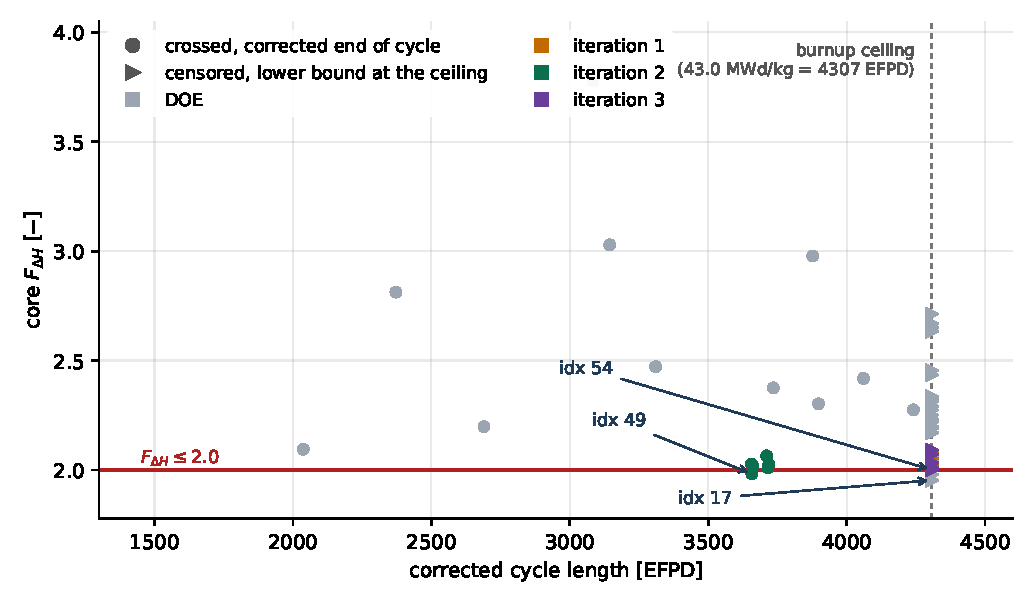
\includegraphics[width=0.95\linewidth]{images/c5_objectives_corrected}
  \caption[Campaign 5 in the corrected objective plane]{Campaign 5 evaluations in the corrected objective plane.}
  \label{fig:c5objcorr}
\end{figure}

Two features of Figure~\ref{fig:c5objcorr} carry the conclusions of the
campaign.

The first is that the ceiling truncates the front. Thirty-nine designs,
including the champion, collapse onto a single cycle-length value, so no
trade-off can be resolved beyond \num{4307} Effective Full Power Days.
The intended ceiling of \SI{75}{\mega\watt\day\per\kilo\gram} was chosen
to sit above every physical end of cycle. The defect silently halved it,
and the corrected value of \SI{43.0}{\mega\watt\day\per\kilo\gram} sits
below the crossing burnup of most of the population. The censoring
lesson of Campaign 2 therefore applies to Campaign 5 in full, through no
choice made in the campaign design.

The second is the identity of the interesting designs, summarised in
Table~\ref{tab:c5-champions}, where feasibility is quoted on both
reactivity bases at the common limit of 1.35. The corrected
non-dominated set consists
of a single design, archive index 17, which pairs the lowest peaking
factor of the entire campaign, $F_{\Delta H} = 1.9534$, with a censored
cycle length of at least \num{4307} Effective Full Power Days. It is a
design-of-experiments point, and the search machinery never treated it
as interesting because its assembly eigenvalue of 1.3764 violates the
as-run reactivity screen. Archive index 49, from the 12-rod lobe, is the
only design in the campaign that combines a sub-limit peaking factor
with a completed, uncensored cycle, at a corrected end of cycle of
\num{3658} Effective Full Power Days, almost exactly ten years at full
power. The campaign champion, index 54, remains the least-infeasible
design under the as-run screens, with the peaking excess of 0.0012 that
the confirmation study of Section~\ref{sec:c5_confirmation} shows to be
statistically indistinguishable from the limit.

\begin{table}[htbp]
  \centering
  \small
  \caption[The three notable designs of Campaign 5]{The three notable designs of Campaign 5 under the corrected objectives. Bold marks a value at a design-space bound.}
  \label{tab:c5-champions}
  \begin{tabularx}{\textwidth}{@{}>{\raggedright\arraybackslash}p{0.27\textwidth}*{3}{>{\centering\arraybackslash}X}@{}}
    \toprule
    Quantity & idx 17, DOE & idx 49, iteration 2 & idx 54, iteration 3 \\
    \midrule
    $e_\mathrm{in}$ / $e_\mathrm{out}$ [wt\%]
      & 16.83 / 14.52 & 7.08 / 7.39 & 13.07 / 15.00 \\
    Gd$_2$O$_3$ content [wt\%]
      & 1.49 & 0.00 & 1.42 \\
    $n_\mathrm{Gd}$ [rods]
      & 32 & \textbf{12} & \textbf{40} \\
    Pitch [cm]
      & 1.154 & \textbf{1.150} & \textbf{1.150} \\
    $t_\mathrm{refl}$ [cm]
      & 17.99 & \textbf{2.00} & 19.41 \\
    Core $F_{\Delta H}$ [--]
      & \textbf{1.9534} & 1.9828 & 2.0012 \\
    Assembly $k_\mathrm{BOL}$ [--]
      & 1.3764 & 1.3574 & 1.3449 \\
    Core $k_\mathrm{eff}$ [--]
      & 1.3060 & 1.2777 & 1.2739 \\
    Corrected cycle length [EFPD]
      & $\geq 4307$ & 3658 & $\geq 4307$ \\
    Feasible, assembly basis
      & no & no & no, by 0.0012 in $F_{\Delta H}$ \\
    Feasible, core basis
      & yes & yes & no, by 0.0012 in $F_{\Delta H}$ \\
    \bottomrule
  \end{tabularx}
\end{table}

The three never-critical designs, archive indices 1, 14 and 22, begin
below their own end-of-cycle targets and therefore fail before the first
depletion step by construction. Their evaluations cost \SI{2.48}{\hour}
in total, 2.3\,\% of the campaign, because the crossing test terminates
them after the beginning-of-life block, at 45 to 57 minutes each against
the campaign mean of 108 minutes. The end-of-cycle test therefore already acts
as an implicit beginning-of-life screen. Making the screen explicit,
\begin{equation}
  g_{k\min} \;=\; k_\mathrm{target}(p,\, t_\mathrm{refl})
  \;-\; k_\mathrm{BOL} \;\leq\; 0 ,
  \label{eq:kmin-selfcons}
\end{equation}

with the terms

\begin{itemize}
  \item $k_\mathrm{BOL}$, the assembly multiplication factor at beginning
        of life, dimensionless,
  \item $k_\mathrm{target}(p,\, t_\mathrm{refl})$, the design-specific
        Route B end-of-cycle target of
        Section~\ref{sec:res-c2}, dimensionless,
\end{itemize}

would reject exactly these three designs before any depletion runs,
recovering the remaining \SI{2.23}{\hour}. Unlike the fixed floor of
1.02, the test contains no arbitrary constant, and it does not reject
archive index 33, a design whose core eigenvalue of 1.011 sits below any
plausible fixed core-level floor yet whose corrected cycle runs to
\num{3084} Effective Full Power Days. The screen is adopted prospectively
for future campaigns and is not applied retrospectively here.

\subsection{Re-scoring the reactivity screen on the core basis}
\label{sec:res-c5-kbasis}

The screening constraint $g_{k\max}$ was applied throughout Campaigns 1
to 5 to the assembly $k_\infty$ of the reflective-boundary depletion
model. Excess reactivity is a budget of the finite core, so the
physically meaningful quantity is the core $k_\mathrm{eff}$, which the
evaluator has recorded for every evaluation since Campaign 4 at no
additional cost. This is the same category distinction that moved the
peaking objective from the assembly to the core in Campaign 4, applied
to the remaining assembly-level constraint. Because both readings exist
in the archives, the question of what the core basis would have changed
is answered by re-scoring, without a single new transport solve.

Figure~\ref{fig:c5kbasis} places every Campaign 4 and Campaign 5
evaluation on the two bases. The points fall in a narrow band displaced
from the identity line by the assembly-to-core gap, and the shaded region
holds the designs that the assembly screen rejects and the core screen
admits at the common limit of 1.35.

\begin{figure}[htbp]
  \centering
  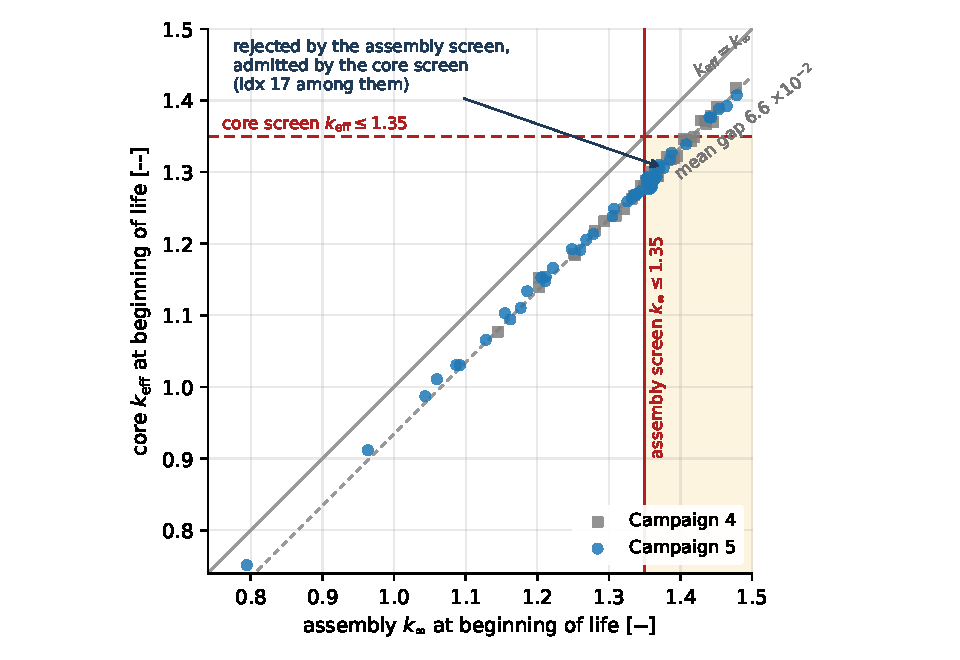
\includegraphics[width=0.82\linewidth]{images/c5_kbasis}
  \caption[The two reactivity bases across Campaigns 4 and 5]{Campaign 4 and Campaign 5 evaluations on the assembly and core reactivity bases.}
  \label{fig:c5kbasis}
\end{figure}

The assembly-to-core gap is large and systematic. Across the Campaign 5
archive it spans \SIrange{4299}{8057}{pcm} with a mean of \SI{6563}{pcm},
and across Campaign 4 it spans \SIrange{5015}{7533}{pcm} with a mean of
\SI{6753}{pcm}. Table~\ref{tab:c5-sweep} sweeps the limit from 1.20 to
1.45 on both bases, with all other constraints held at their campaign
values.

\begin{table}[htbp]
  \centering
  \small
  \caption[Feasible designs under both reactivity bases]{Number of designs satisfying all five screening constraints against the reactivity limit on each basis.}
  \label{tab:c5-sweep}
  \begin{tabular}{c cc cc}
    \toprule
    & \multicolumn{2}{c}{Campaign 4 (54)} &
      \multicolumn{2}{c}{Campaign 5 (60)} \\
    \cmidrule(lr){2-3}\cmidrule(lr){4-5}
    $k$ limit & assembly & core & assembly & core \\
    \midrule
    1.20 & 0 & 0 & 0 & 0 \\
    1.25 & 0 & 0 & 0 & 0 \\
    1.30 & 0 & 6 & 0 & 1 \\
    1.35 & 0 & 7 & 0 & 2 \\
    1.40 & 7 & 7 & 2 & 3 \\
    1.45 & 7 & 7 & 2 & 3 \\
    \bottomrule
  \end{tabular}
\end{table}

Three findings follow.

First, the two formulations that have been under discussion select
identical designs. The core basis at 1.35 admits archive indices 6, 42,
43, 44, 46, 47 and 53 in Campaign 4 and indices 17 and 49 in Campaign 5.
The assembly basis at 1.40 admits exactly the same sets, in both
campaigns. The relaxation to 1.40 and the change of basis are therefore
interchangeable in outcome, and only their justification differs. The
basis change rests on the measured gap and on the physical location of
the excess-reactivity budget, so it is the route adopted here.

Second, the tangency reading of Campaign 4 in
Section~\ref{sec:res-c4-trajectory} does not survive the re-scoring. On
the core basis at 1.35, every one of the 47 infeasible Campaign 4
designs violates the peaking constraint, so $g_{k\max}$ excludes no
design that $g_\mathrm{peak}$ would have admitted. The two constraints
are not tangent. There is a single peaking wall, and the apparent second
wall was the reactivity screen evaluated on a quantity that sits
approximately \SI{6800}{pcm} above the budgeted one. The same holds in
Campaign 5 with a single exception, archive index 16, which passes
peaking at 1.9796 and fails reactivity on both bases. Re-read on the
core basis, the Campaign 4 active learning was more successful than the
as-run accounting showed: its second iteration placed five of six
proposals inside the feasible region, and the third iteration then moved
away from it, because the violation being minimised was computed on the
assembly quantity.

Third, the campaign comparison inverts. Under the as-run screens both
campaigns report zero feasible designs and Campaign 5 reports the
smaller closest approach. Under the core basis Campaign 4 holds seven
feasible designs against two, despite the smaller design space. The
infill pressure toward high absorber inventory, exerted by a reactivity
screen evaluated on the wrong quantity, drove part of the Campaign 5
search into the never-critical region documented above. A constraint
defined on a proxy therefore did not merely mislabel the results. It
steered the search. This is the same failure mode established for the
peaking proxy in Section~\ref{sec:res-corevalidation}, observed a second
time in an independent constraint, which elevates it from an anecdote to
a property of proxy-constrained surrogate optimisation in this design
space.

The limit itself remains a screening value. On the core basis, a
multiplication factor of 1.35 corresponds to approximately
\SI{25900}{pcm} of excess reactivity to be held by the burnable
absorber, the \SI{1000}{ppm} soluble boron of the benchmark basis and
the control rods.

Whether that budget is controllable is a rod-worth question, and
Campaign 7 answers it by measurement. Deriving the ceiling from the
measured worth of all seven banks with a \SI{1000}{pcm} operating
margin gives 1.368 (Section~\ref{sec:res-c7-worth}), so the value of
1.35 used in Campaigns 1 to 6 is the all-bank controllability bound of
this core to within two per cent.

The regulating banks alone hold down considerably less, and from
Campaign 7 the ceiling is replaced as the working constraint by the
measured controllability screen of Section~\ref{sec:meth-ctrl}.

The remaining gap in peaking between this single-batch uniform core and
licensed practice, where a Technical Specification limit of 1.65 on
$F_{\Delta H}$ applies~\cite{robinson_gd10}, is the domain of
multi-batch loading patterns, zoned absorber placement and rod
programmes~\cite{kropaczek_turinsky_1991,aga_firstcore_2021,chasnupp_lpo_2013}.
Those are outside this design space by construction and are the
natural continuation of the work (Section~\ref{sec:concl-future}).

\subsection{High-fidelity confirmation of the Campaign 5 champion}
\label{sec:c5_confirmation}

Campaign 5 returned no design satisfying every as-run screening
constraint in sixty evaluations. The least-infeasible design, archive
index 54, violated only the radial enthalpy-rise constraint, and by an
amount smaller than the run-to-run scatter of the Monte Carlo estimator
that produces it. A separate confirmation study was therefore run to
determine whether that violation is a property of the design or an
artefact of the transport statistics.

The design was re-solved at beginning of life with eight independent
transport seeds at raised fidelity, namely \num{200000} particles per batch
over 260 batches with 80 inactive batches, against the campaign setting of
\num{100000} particles over 170 batches with 60 inactive batches. The
assembly eigenvalue was re-solved with four independent seeds. No depletion
was repeated, because the peaking factor is a beginning-of-life quantity and
the cycle length of this design is set by the burnup ceiling rather than by
the reactivity target. The peaking estimator, the mesh definition and the
Shannon-entropy source-convergence diagnostic were taken unchanged from the campaign
evaluator, so the confirmed quantity is identical in definition to the
optimisation objective.

The sample statistics are formed as

\begin{equation}
\bar{F} = \frac{1}{n}\sum_{i=1}^{n} F_i ,
\qquad
s = \sqrt{\frac{1}{n-1}\sum_{i=1}^{n}\left(F_i - \bar{F}\right)^2 },
\qquad
\mathrm{CI}_{95} = \bar{F} \pm t_{0.975,\,n-1}\,\frac{s}{\sqrt{n}} ,
\end{equation}

with the terms

\begin{itemize}
  \item $F_i$, the radial enthalpy-rise hot channel factor returned by
        transport seed $i$, dimensionless,
  \item $n$, the number of independent seeds, dimensionless,
  \item $\bar{F}$, the sample mean of the peaking factor, dimensionless,
  \item $s$, the sample standard deviation of the peaking factor,
        dimensionless,
  \item $t_{0.975,\,n-1}$, the two-sided Student critical value at the
        \SI{95}{\percent} level with $n-1$ degrees of freedom, dimensionless.
\end{itemize}

The design was declared feasible on a constraint only when the entire
confidence interval clears the limit, which is the conservative test.
Table~\ref{tab:c5_confirmation} gives the result for the champion. The
peaking constraint cannot be separated from its limit.

\begin{table}[htbp]
  \centering
  \caption[Campaign 5 champion confirmed at raised fidelity]{Campaign 5 champion, archive index 54, confirmed at raised fidelity.}
  \label{tab:c5_confirmation}
  \begin{tabular}{lrrrrl}
    \toprule
    Quantity & Mean & $s$ & \multicolumn{2}{c}{\SI{95}{\percent} interval}
             & Verdict \\
    \midrule
    Core $F_{\Delta H}$ ($n=8$)      & 2.00350 & 0.01320 & 1.99246 & 2.01454
                                     & indistinguishable \\
    Assembly $k_{\mathrm{BOL}}$ ($n=4$) & 1.34392 & 0.00030 & 1.34344 & 1.34440
                                     & pass \\
    Core $k_{\mathrm{eff}}$ ($n=8$)  & 1.27424 & --      & --      & --
                                     & not constrained \\
    \bottomrule
  \end{tabular}
\end{table}

The reactivity constraint is settled. The assembly eigenvalue clears the
screening limit of 1.35 by \SI{608}{pcm}, against a seed-to-seed standard
deviation of \SI{30}{pcm}, so the margin exceeds twenty standard errors. The
core eigenvalue of the same design is \SI{6968}{pcm} below the assembly
value, consistent with the range of \SIrange{5012}{7530}{pcm} measured across
the Campaign 4 archive, which confirms that the screening limit is applied to
the more conservative of the two quantities.

The peaking constraint is not settled, and cannot be settled at this
resolution. The mean exceeds the limit of 2.0 by 0.0035, which is
\SI{0.175}{\percent} of the limit and approximately one quarter of one
standard deviation of a single solve. Individual seeds fall on both sides of
the limit, spanning 1.9843 to 2.0217. Reducing the standard error far enough
for the interval to separate from the limit at the observed offset would
require of the order of fifty-five independent seeds, and would establish a
violation of less than two tenths of one percent of a bound that is itself a
relaxed screening value rather than a licensed limit.

Two observations on the estimator follow from the same data set. The
campaign evaluation of this design returned 2.0012 at the lower campaign
fidelity, which falls at the 38th percentile of the eight high-fidelity
seeds, so no fidelity bias is detectable in the optimisation objective. The
measured standard deviation is 1.33 times the value predicted by inverse
square-root scaling of the particle count from the Campaign 3 noise
measurement. This is expected behaviour, because the peaking factor is a
maximum over mesh bins rather than a mean, and extreme-value statistics
converge more slowly than sample means with increasing particle count.

%% AUTHOR: physics interpretation of the gadolinia pin count as the mechanism
%% that moved the constraint boundary without opening an overlap on the
%% as-run basis, read together with the corrected picture of
%% Section~\ref{sec:res-c5-corrected} in which archive indices 17 and 49
%% are feasible on the core basis.

The conclusion for the design space is therefore threefold. Adding the
gadolinia-bearing rod count as a sixth design variable lowered the
minimum total constraint violation from 0.0077 in Campaign 4 to 0.0012
in Campaign 5, so the additional degree of freedom measurably moved the
constraint boundary on the as-run basis. On that basis the best
reachable design lies on the peaking boundary to within the resolution
of the model. On the core reactivity basis of
Section~\ref{sec:res-c5-kbasis}, two designs of this campaign and seven
of the previous one are feasible, and the sole remaining obstacle in the
design space is the peaking wall. Under uniform loading no
distinguishable peaking margin exists beyond it, which motivates the
zoned-loading study as the natural continuation of the work.

% ===================== end of replacement block ======================

\subsection{A defect in the restarted depletion}
\label{sec:restart_defect}

\subsubsection{Depletion in separate blocks}

The depletion solver requires the complete list of burnup steps before the
calculation starts. A single call of the form "burn six steps of
\SI{4}{\mega\watt\day\per\kilo\gram}" runs to the end of that list and
stops.

This requirement conflicts with the definition of the cycle length used in
this work. The end of cycle is the burnup at which the reactivity falls to
the target value, and that burnup is not known before the calculation is
performed, because it is a property of the design being evaluated.

Supplying a fixed list is therefore either insufficient or wasteful. A short
list may end while the reactivity is still far above the target, in which
case the design has not been evaluated at all. A long list continues to burn
fuel after the target has been crossed, at a cost of several minutes of
computing time per unnecessary step. Across the enrichment range explored by
the campaigns, no single fixed list is appropriate for every design.

The evaluator therefore advances the depletion in short blocks and inspects
the reactivity after each one. It continues only while the target has not
been crossed and the burnup ceiling has not been reached. Each block is a
separate call to the depletion solver, and the number of blocks adapts to
the design.

Archive index 7 illustrates the resulting structure. Its depletion consists
of nine blocks:

\begin{enumerate}
  \item the first block advances five steps of 0.5, 1.0, 2.0, 4.0 and
        \SI{6.0}{\mega\watt\day\per\kilo\gram}, reaching
        \SI{13.5}{\mega\watt\day\per\kilo\gram},
  \item the second through eighth blocks each advance two steps of
        \SI{4.0}{\mega\watt\day\per\kilo\gram},
  \item the ninth block advances \SI{4.0}{} and then
        \SI{1.5}{\mega\watt\day\per\kilo\gram}, stopping at the burnup
        ceiling rather than at a reactivity crossing.
\end{enumerate}

\subsubsection{How one block continues from the previous one}

Consecutive blocks are not independent calculations. Each block must begin
with the fuel in exactly the state the previous block left it, including the
depleted uranium content, the accumulated plutonium and the fission product
inventory.

The continuation is performed through the results file. A block writes its
final state to disk, and the next block reads that file and passes it to a
new depletion operator as the previous state. This operation is referred to
here as a restart. The nine blocks of archive index 7 therefore involve
eight restarts.

A results file is expected to carry two distinct kinds of information:

\begin{enumerate}
  \item the material composition, which specifies how much of each nuclide
        is present,
  \item the reaction rates, which specify how rapidly each nuclide is being
        transmuted at the current flux level.
\end{enumerate}

The composition tells the solver where the fuel is. The reaction rates tell
it how fast the fuel is changing. A restart requires both, because the first
step after a restart is advanced using the reaction rates carried over from
the end of the previous block.

\subsubsection{Origin of the restart defect}

Version 0.15.3 of the depletion solver introduced an option controlling
whether reaction rates are written to the results file, and set its default
to false in order to reduce file size. The evaluator did not set this
option, so the results files written by every block contained the material
composition but no reaction rates.

A results object reconstructed from such a file carries an empty reaction
rate structure, because the reconstruction relies on metadata that is absent
from the file. The restart routine reads that structure and passes it to the
solver without verifying that it is populated.

The consequence is that the first step of every restarted block was advanced
with all transmutation channels set to zero. The material composition
evolved by radioactive decay alone. No fission occurred, no fission products
were produced, and no burnup was accumulated. The burnup label maintained by
the evaluator was nevertheless advanced by the full step.

The failure was silent. The calculation completed without error, and every
value it returned was of a plausible magnitude.

\subsubsection{The signature in the recorded history}

Figure~\ref{fig:restart_defect}(a) shows the depletion history of archive
index 7 as the evaluator recorded it. The points separate into two branches
approximately \SI{950}{pcm} apart.

The upper branch consists of the first point of every restarted block. These
are the steps in which the fuel did not burn. Physical time advanced
nonetheless, so xenon-135 decayed without being replaced by fission and the
reactivity rose. The measured rises are 1040, 1029, 963, 1232, 926, 1019,
732 and \SI{670}{pcm}, with a mean of \SI{951}{pcm} and a standard deviation
of \SI{179}{pcm}. A positive reactivity excursion of this magnitude,
occurring exclusively at block boundaries and nowhere else, is
characteristic of xenon removal and is not consistent with any depletion
process.

The lower branch consists of the second point of every block. These points
are physically correct. Their burnup labels, however, have advanced twice as
fast as the fuel. Figure~\ref{fig:restart_defect}(b) plots the same
measured reactivities against the burnup the fuel actually reached,
together with an independent control calculation performed as a single
uninterrupted block, and the corrected trajectory agrees with the control
calculation.

\begin{figure}[htbp]
  \centering
  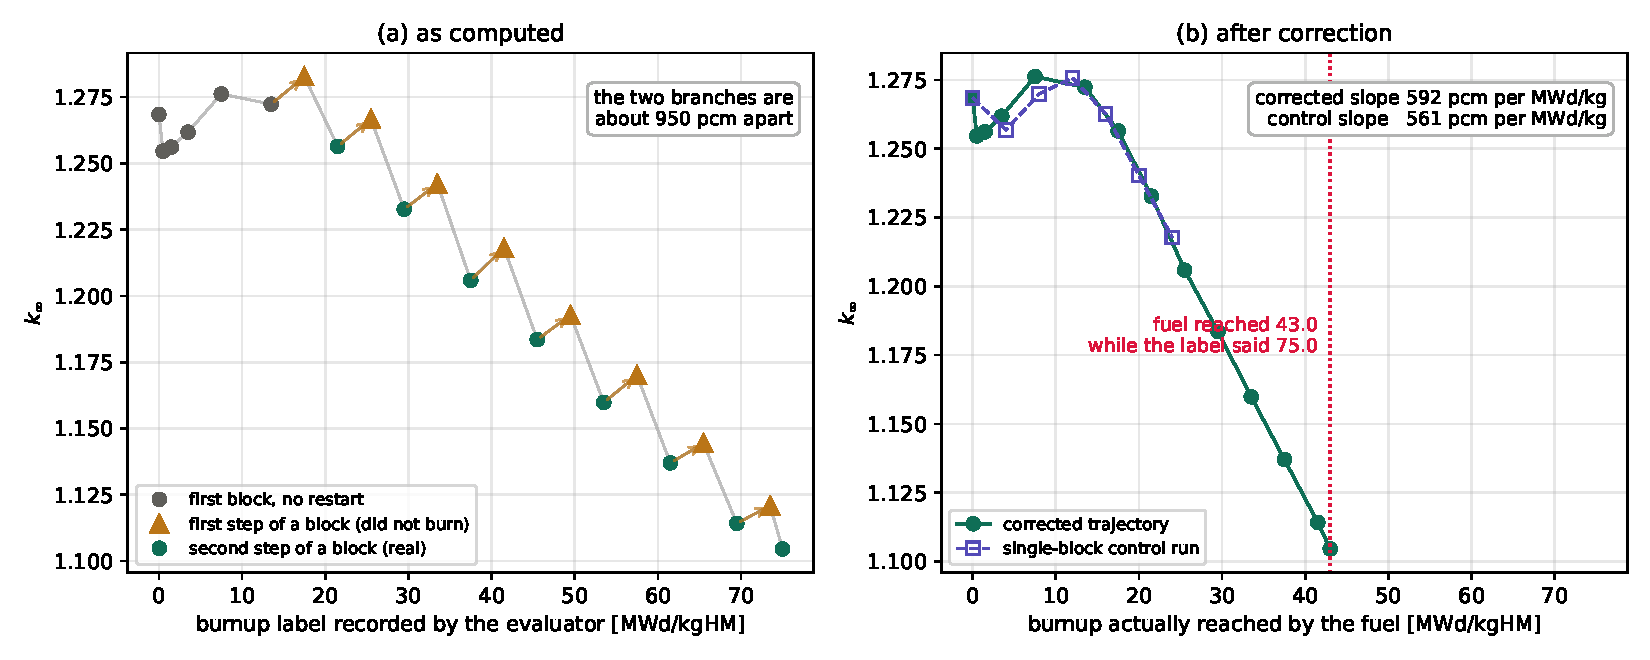
\includegraphics[width=\textwidth]{images/fig_restart_defect.pdf}
  \caption[Depletion history of archive index 7]{Depletion history of archive index 7. (a)~As recorded. (b)~Against the burnup actually reached, with the control calculation.}
  \label{fig:restart_defect}
\end{figure}

\subsubsection{The controlled experiment}

The mechanism was confirmed by depleting archive index 7 twice through the
same model and the same random seed, with the only difference being the
block structure:

\begin{enumerate}
  \item arm A, a single uninterrupted block of six steps of
        \SI{4}{\mega\watt\day\per\kilo\gram},
  \item arm B, three blocks of two steps covering the identical burnup
        points.
\end{enumerate}

Because the model and the seed are shared, the two arms compute the same
quantity at every point and must agree to within the statistical scatter of
the transport solution. Table~\ref{tab:restart_experiment} compares the
two arms.

\begin{table}[htbp]
  \centering
  \caption{Reactivity of archive index 7 computed with and without block restarts.}
  \label{tab:restart_experiment}
  \begin{tabular}{rrrrl}
    \toprule
    Burnup label & Arm A & Arm B & Difference & Position \\
    $[$\si{\mega\watt\day\per\kilo\gram}$]$ & $k_\infty$ & $k_\infty$
      & [\si{pcm}] & \\
    \midrule
     0 & 1.26846 & 1.26846 &    0 & start \\
     4 & 1.25680 & 1.25736 &  +56 & before any restart \\
     8 & 1.26988 & 1.27067 &  +79 & first restart point \\
    12 & 1.27568 & 1.28094 & +526 & first step after a restart \\
    16 & 1.26267 & 1.27436 & +1169 & second restart point \\
    20 & 1.24028 & 1.28461 & +4433 & first step after a restart \\
    24 & 1.21775 & 1.26382 & +4607 & final point \\
    \bottomrule
  \end{tabular}
\end{table}

Table~\ref{tab:restart_experiment} supports the mechanism in two independent
ways.

The first is the location of the divergence. At 0, 4 and
\SI{8}{\mega\watt\day\per\kilo\gram} the two arms differ by 0, 56 and
\SI{79}{pcm}, which is the ordinary scatter of the transport solution at the
campaign settings. Divergence begins at exactly
\SI{12}{\mega\watt\day\per\kilo\gram}, the first point computed after the
first restart, and grows monotonically thereafter.

The second is the size of the divergence. If each restart consumes one step
without burning the fuel, then the arm B point labelled 16 is the true state
at 12, and the point labelled 24 is the true state at 16. The measured
values are 1.27436 against 1.27568, a difference of \SI{-132}{pcm}, and
1.26382 against 1.26267, a difference of \SI{115}{pcm}. Both lie inside the
statistical scatter. The chunked calculation is therefore not incorrect in
an unstructured way. It is behind by exactly one step per restart.

\subsubsection{Correcting the recorded histories}

For blocks of two steps, the burnup label advances twice as fast as the
fuel. The relation between the two is

\begin{equation}
B_{\mathrm{true}} = B_{0} + \frac{B_{\mathrm{label}} - B_{0}}{2} ,
\label{eq:true_burnup}
\end{equation}

with the terms

\begin{itemize}
  \item $B_{\mathrm{label}}$, the cumulative burnup recorded by the
        evaluator, in \si{\mega\watt\day\per\kilo\gram} of heavy metal,
  \item $B_{\mathrm{true}}$, the burnup physically reached by the fuel, in
        the same units,
  \item $B_{0}$, the burnup at the end of the first block, which contains no
        restart and is therefore unaffected, equal to
        \SI{13.5}{\mega\watt\day\per\kilo\gram} for the schedule used here.
\end{itemize}

Figure~\ref{fig:restart_defect}(b) applies this correction. The points of
the upper branch are discarded, because they duplicate the state preceding
them, and the remaining points are relabelled. The two branches collapse
onto a single smooth trajectory.

Two quantitative checks confirm the correction. The corrected trajectory
falls at \SI{592}{pcm} per unit of burnup, against \SI{561}{pcm} measured in
the independent single-block control calculation, an agreement of
\SI{5}{\percent}. The control calculation itself is plotted in
Figure~\ref{fig:restart_defect}(b) and lies on the corrected trajectory.

Applying Equation~\ref{eq:true_burnup}, the reported ceiling of
\SI{75.0}{\mega\watt\day\per\kilo\gram} for archive index 7 corresponds to a
physical burnup of \SI{43.0}{\mega\watt\day\per\kilo\gram}. The reported
cycle length of \num{7513} Effective Full Power Days corresponds to
\num{4307}, an overstatement by a factor of 1.74.

\subsubsection{Scope of the affected results}

The defect affects only quantities that depend on depletion beyond the first
block. The following results are unaffected and require no revision:

\begin{itemize}
  \item all beginning of life quantities, including every core radial
        peaking factor and every assembly eigenvalue at zero burnup,
  \item the transfer test and the multiplier optimisation of the
        zoned-loading study, whose multipliers now enter the
        methodology in Section~\ref{sec:meth-zoning} and which are
        computed at beginning of life. Its Stage 3 confirmation does
        deplete, but both runs completed after the correction was
        committed, as recorded in Section~\ref{sec:meth-zoning-study},
  \item the feasibility assessment against the peaking constraint and
        against the beginning of life reactivity constraint.
\end{itemize}

The following results require correction:

\begin{itemize}
  \item every cycle length obtained from a trajectory that crossed the
        reactivity target, which is overstated,
  \item every burnup reported at the ceiling, which is overstated by
        Equation~\ref{eq:true_burnup},
  \item every reactivity slope derived from the affected histories, which is
        understated by approximately a factor of two.
\end{itemize}

The depletions do not need to be repeated. The physical states already
computed are correct and only their burnup labels are wrong, so the archived
histories can be corrected by discarding the first entry of each block and
applying Equation~\ref{eq:true_burnup}.

The solver version question is closed. The pinned environments of
Section~\ref{sec:meth-diagnostics} carry OpenMC 0.15.3 on both hosts
for every campaign, so Campaigns 1 to 5 all executed under the
affected default and the correction applies to the whole archive.
Campaign 6 is the first campaign to run entirely under the corrected
configuration, and its checkpoint metadata records the setting.

\subsubsection{Correction applied to the evaluator}

The evaluator was modified to request that reaction rates be written to the
results file. A verification was added that raises an error if a results
object about to be used for a restart carries an empty reaction rate
structure. The verification is deliberately fatal rather than advisory,
because the condition it detects produces physically plausible output and
would otherwise remain undetected.

The controlled experiment of Table~\ref{tab:restart_experiment} was repeated
after the correction as an acceptance test, with the criterion that the two
arms agree at every point to within the statistical scatter of the transport
solution.

%% AUTHOR: state the physical interpretation of the corrected cycle lengths
%% and their relation to the fuel burnup limits discussed in the constraint
%% sourcing section, noting that the corrected ceiling burnup of
%% 43.0 MWd/kgHM lies below both the 62 GWd/t rod average and the
%% 55 GWd/t assembly average values.

\subsubsection{Methodological observation}

This is the fourth defect in this work identified by subjecting the model to
a condition its author had not anticipated, following an inconsistency in a
geometric padding constant, a failure of the optimiser when no feasible
design exists, and an incorrect reading of the output of a restarted
depletion. In each case the calculation completed without error and returned
values of plausible magnitude.

The common feature is that each defect was exposed by a deliberate
consistency test rather than by inspection of the source code. The present
case is the strongest instance, because the defect arises in a widely used
external code operating in its default configuration, and the test that
revealed it consists of performing the same calculation in two ways that
must agree.

%% AUTHOR: decide whether to report this defect to the maintainers of the
%% depletion solver, and if so, cite the report here.

\section{Campaign 6: the corrected basis and the acquisition programme}
\label{sec:res-c6}
\label{sec:res-c6-blocks}

Campaign 6 applies the three corrections established by the Campaign 5
analyses, namely the core-basis reactivity window, the evaluator-level
radial zoning and the raised depletion horizon, and then uses the
campaign itself as a controlled test bench for the acquisition
function. The campaign comprises \num{114} evaluations in five blocks.
The design of experiments is followed by four infill blocks, and each
infill block changes exactly one element of the acquisition of
Section~\ref{sec:meth-acq}, so every behavioural change is
attributable. Table~\ref{tab:c6-blocks} gives the block structure, with
the hypervolume taken as the archive value against the frozen reference
point after the last iteration of each block.

\begin{table}[htbp]
  \centering
  \small
  \caption{Campaign 6 block structure.}
  \label{tab:c6-blocks}
  \begin{tabularx}{\textwidth}{@{}lcc>{\raggedright\arraybackslash}Xc@{}}
    \toprule
    Block & Evaluations & Feasible & Acquisition state & Hypervolume \\
    \midrule
    1, DOE & 42 & 28 & none, Latin hypercube          & 1288.09 \\
    2      & 18 & 13 & bare uncertainty ranking       & 1288.09 \\
    3      &  6 &  1 & + batch diversity              & 1288.09 \\
    4      & 18 & 17 & + feasibility margin           & 1580.05 \\
    5      & 30 & 29 & unchanged, convergence check   & 1601.51 \\
    \bottomrule
  \end{tabularx}
\end{table}

\subsection{Design of experiments}
\label{sec:res-c6-doe}

The 42-point Latin hypercube returned 28 feasible designs, against
zero in the Campaign 5 design of experiments of identical size. Every
rejection is fully explained by the active constraints.

\begin{itemize}
  \item Ten designs exceed the peaking limit of 2.0.

  \item Five designs fall below the reactivity floor of 1.02 on the
        core basis, including one that never reaches criticality at
        all, with $k_\mathrm{eff}^\mathrm{core} = 0.817$.

  \item Two designs exceed the reactivity ceiling of 1.35.

  \item No design violates the zoned enrichment cap, which the search
        box of Equation~\eqref{eq:leu-box} guarantees by construction.

  \item Four designs violate two constraints simultaneously, which
        reconciles the counts with the 14 rejections.
\end{itemize}

The floor rejections are the first practical consequence of the basis
change. On the assembly basis of Campaigns 1 to 5 the floor of 1.02
never acted. On the core basis it rejects genuinely subcritical cores,
which answers the standing question of whether that bound carries any
physical content.

The Pareto front of the design of experiments holds two designs, at
\num{9445} effective full power days with $F_{\Delta H} = 1.6554$ and
at \num{9035} with $F_{\Delta H} = 1.5741$. Exactly one design
censored at the ceiling, at \num{10016.7} effective full power days
and \SI{100.0}{\mega\watt\day\per\kilo\gram}, and it is infeasible on
the reactivity ceiling in any case.

The frozen hypervolume reference point is constructed from this
two-design front by the nadir-plus-offset rule, at \num{6776}
effective full power days and 2.0692 in peaking. The consequences of
freezing the reference on so small a front are examined in
Section~\ref{sec:res-c6-margin}.

\subsection{Blocks 2 and 3: two acquisition defects, measured}
\label{sec:res-c6-defects}

\subsubsection{Block 2: batch collapse}

Block 2 ran the bare uncertainty ranking of
Equation~\eqref{eq:acq-score} for three iterations of six evaluations.
The batches collapsed. Within each iteration the six selected designs
are near copies of one design, and the eighteen evaluations bought
three distinct design points. The second iteration is representative.
Table~\ref{tab:c6-b2-collapse} lists its six designs. The inner
enrichment spans 0.03~wt\%, the pitch is identical to three decimals in
five of the six, and the reflector spans \SI{0.1}{\centi\metre}.

\begin{table}[htbp]
  \centering
  \caption{Campaign 6, block 2, iteration 2: the six infill designs.}
  \label{tab:c6-b2-collapse}
  \begin{tabular}{cccccc}
    \toprule
    Index & $e_\mathrm{in}$ (wt\%) & $e_\mathrm{out}$ (wt\%) &
    $p$ (cm) & $t_\mathrm{refl}$ (cm) & EFPD \\
    \midrule
    48 & 4.42 & 3.77 & 1.380 & 5.4 & 2011 \\
    49 & 4.44 & 3.77 & 1.380 & 5.4 & 2002 \\
    50 & 4.45 & 3.83 & 1.380 & 5.4 & 2047 \\
    51 & 4.45 & 3.82 & 1.380 & 5.4 & 2053 \\
    52 & 4.43 & 3.77 & 1.380 & 5.4 & 2009 \\
    53 & 4.42 & 3.75 & 1.381 & 5.3 & 1985 \\
    \bottomrule
  \end{tabular}
\end{table}

Two mechanisms combine. The top of a smooth uncertainty field is a
neighbourhood, so the six highest-scoring candidates are adjacent, and
the duplicate test then in force compared raw design vectors at a
tolerance of $10^{-6}$, which only exact numerical copies can fail.
Designs 0.01~wt\% apart passed it four orders of magnitude clear.

The hypervolume did not move in any of the three iterations. The front
nevertheless grew from two designs to six, entirely at the short-cycle
end, including the first design of the whole programme to clear the
1.50 licensing-style screen, at $F_{\Delta H} = 1.4041$ and \num{1054}
effective full power days. The frozen reference point sits at
\num{6776} effective full power days, so every one of these additions
contributes exactly zero to the reported metric. Recomputed against a
full-range reference the archive hypervolume rises from \num{4643} to
\num{4876} across the block, which quantifies what the frozen metric
hides.

\subsubsection{Block 3: constraint blindness}

Block 3 added the batch-diversity separation of
Equation~\eqref{eq:batch-div} at $\delta_\mathrm{min} = 0.10$ and
nothing else. The separation worked as designed. The six picks are
distinct, the pitch spans its full box and the reflector spans
\num{2.0} to \SI{19.5}{\centi\metre}, and no relaxation was required.

With the collapse removed, the next defect became visible. Five of the
six designs returned infeasible on the reactivity ceiling.
Table~\ref{tab:c6-b3-fail} lists the outcomes, with the margin taken as
the excess of $k_\mathrm{eff}^\mathrm{core}$ over the ceiling of 1.35.

\begin{table}[htbp]
  \centering
  \caption{Campaign 6, block 3: infill outcomes.}
  \label{tab:c6-b3-fail}
  \begin{tabular}{ccccc}
    \toprule
    Index & EFPD & $F_{\Delta H}$ & $k_\mathrm{eff}^\mathrm{core}$ &
    Margin (pcm) \\
    \midrule
    60 & 3776 & 1.6430 & 1.29510 & feasible \\
    61 & 8167 & 1.7288 & 1.36533 & $+1533$ \\
    62 & 8395 & 1.7380 & 1.37574 & $+2574$ \\
    63 & 9023 & 1.7324 & 1.39692 & $+4692$ \\
    64 & 9806 & 1.8328 & 1.42680 & $+7680$ \\
    65 & 9728 & 1.7408 & 1.42745 & $+7745$ \\
    \bottomrule
  \end{tabular}
\end{table}

The mechanism is visible in one column of the archive. The gadolinia
content of all six designs is exactly zero. The objective surrogate had
learned that the absorber costs cycle length and drove it out, the
enrichments rose toward the box ceiling, and nothing remained to hold
beginning-of-life reactivity inside the window. The constraint
surrogate predicted feasibility for all five failures even though the
archive already contained a design at
$k_\mathrm{eff}^\mathrm{core} = 1.402$ in that corner. The
Gaussian-process mean is optimistic where the data is thin, and the
bare acquisition never asked it for margin.

\subsection{Blocks 4 and 5: the margin and the convergence}
\label{sec:res-c6-margin}

Block 4 added the feasibility margin of
Equation~\eqref{eq:feas-margin} at $\kappa = 1.5$ and nothing else.
The effect was immediate on all three indicators.

\begin{enumerate}
  \item Seventeen of eighteen designs returned feasible. The single
        failure exceeds the ceiling by \num{151}\,pcm, against
        \num{1533} to \num{7745} in block 3. The search moved from
        wandering deep into the forbidden region to riding the
        constraint boundary.

  \item The gadolinia returned, at 1.57 to 3.30~wt\% in the first
        iteration, then probing the upper bound at 7.92 to 8.00, then
        the dilute alternative at 0.64 to 0.70. The optimiser was
        mapping the absorber trade rather than deleting it.

  \item The hypervolume moved for the first time in the campaign, from
        1288.09 to 1525.01, then 1548.33, then 1580.05, gains of
        18.39, 1.53 and 2.05 per cent.
\end{enumerate}

The margin filter also behaved as a learning indicator. The number of
margin-feasible candidates out of 300 moved from 257 to 168 to 202
across the three iterations, tightening when the first batch taught
the constraint surrogate about the high-enrichment corner and
loosening as further evidence accumulated.

Block 5 changed nothing in the acquisition and ran five iterations at
$\delta_\mathrm{min} = 0.14$ as a convergence check. The hypervolume
gains were 0.60, 0.49, 0.21, 0.05 and 0.02 per cent, five consecutive
iterations below the one per cent threshold. The single censored
design of the archive is infeasible and off the front, so both
conditions of the stopping rule of Section~\ref{sec:meth-loop} are
met and the campaign terminates at \num{114} evaluations.

Two independent signals corroborate the termination.

\begin{enumerate}
  \item The diversity relaxation cascade deepened monotonically. The
        first block 5 iteration already needed relaxation to 0.0175 to
        fill its batch, and the fifth found not a single candidate
        even at that value and completed below 0.009. The surrogate
        front no longer contains materially new designs.

  \item The margin-feasible count rose monotonically from 160 to 266
        of 300, so the constraint surrogate had stopped revising its
        map of the feasible region.
\end{enumerate}

The same stopping rule had already fired once before, falsely. After
block 3 the campaign showed three consecutive iterations at exactly
zero gain while the acquisition was demonstrably selecting duplicates
and then constraint violations. Read literally, the rule declared a
broken search converged. The two firings differ in every indicator
except the hypervolume itself, which is the experimental basis for
treating the rule as necessary and not sufficient, and for the health
indicators added to Section~\ref{sec:meth-loop}.

The two settings established across blocks 4 and 5, the feasibility
margin of 1.5 standard deviations and the minimum separation of 0.14,
were not passed to the Campaign 7 launcher. Two of that campaign's
three infill blocks collapsed in exactly the way documented for blocks
2 and 3 above (Section~\ref{sec:res-c7-blocks}). Both settings are
stated explicitly on the command line from Campaign 8, and a flat
hypervolume is read as a stopping signal only when the acquisition is
known to be functioning.

Figure~\ref{fig:c6-convergence} shows the archive hypervolume after every
evaluation, under the frozen in-campaign reference in the top panel and
under a full-range reference in the bottom panel, with the five blocks
shaded. The frozen metric is flat through blocks 2 and 3 while the
full-range metric shows their genuine short-cycle contribution, and the
first improvement visible to the frozen metric coincides exactly with the
feasibility margin of block 4.

\begin{figure}[htbp]
  \centering
  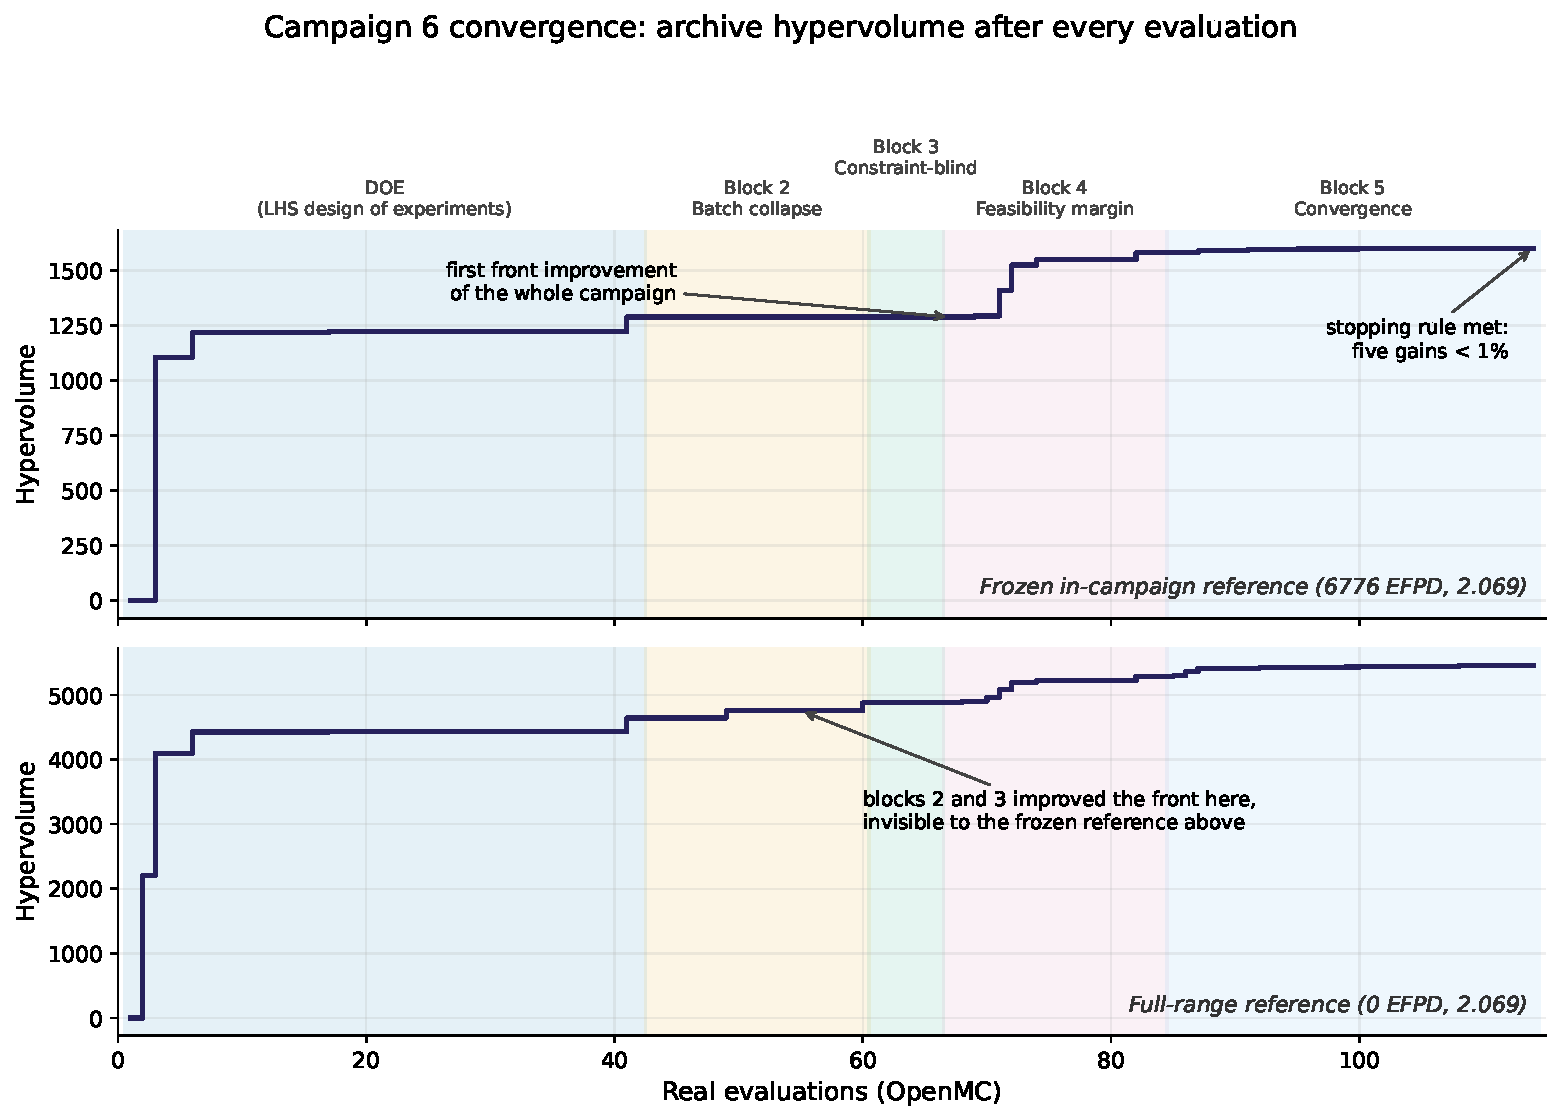
\includegraphics[width=\linewidth]{images/c6_extra_convergence}
  \caption{Campaign 6 convergence: archive hypervolume under the frozen and the full-range reference points.}
  \label{fig:c6-convergence}
\end{figure}

\subsection{The resolved front}
\label{sec:res-c6-front}

Figure~\ref{fig:c6-front} shows the objective space after \num{114}
evaluations. Feasible designs are coloured by block, infeasible designs
are crosses in the colour of their block, and the step line is the
Pareto front of the feasible set. The frozen hypervolume reference point
and the licensing-style screens at 1.65 and 1.50 are drawn for context.

\begin{figure}[htbp]
  \centering
  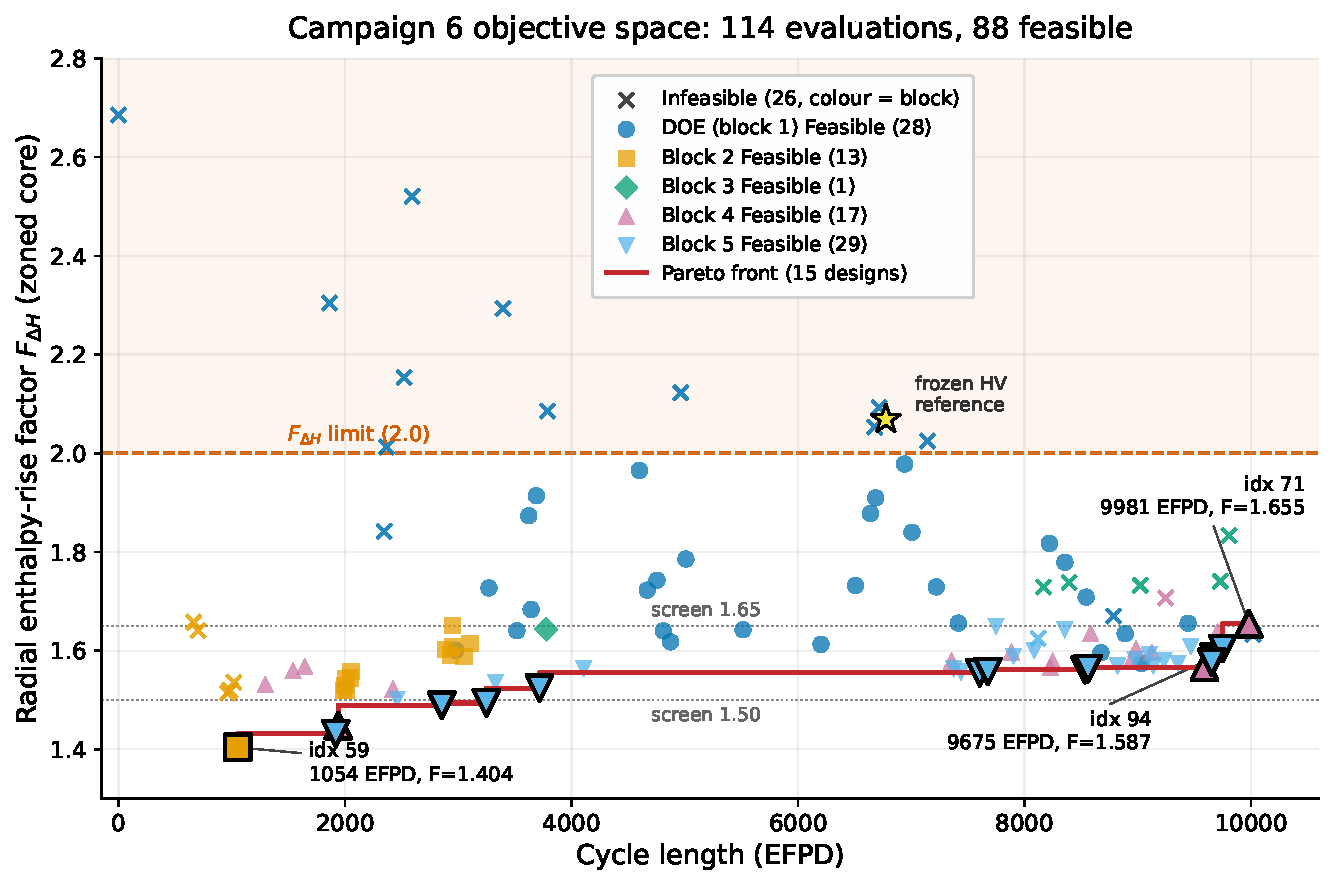
\includegraphics[width=\linewidth]{images/c6_pareto_front_114}
  \caption{Campaign 6 objective space after \num{114} evaluations.}
  \label{fig:c6-front}
\end{figure}

The final front holds fifteen designs and spans the full trade, from
\num{1054} effective full power days at $F_{\Delta H} = 1.4041$ to
\num{9981} at 1.6547 (Table~\ref{tab:c6-front}). In the table the
peaking factor is the zoned-core beginning-of-life value, the eigenvalue
is on the core basis and the burnup is the end-of-cycle value. The pin
count is omitted because every front design carries 40
gadolinium-bearing pins, and the cycle lengths are two-dimensional
exploration-tier values in the sense of Sections~\ref{sec:meth-fidelity}
and~\ref{sec:meth-lax}.

\begin{table}[htbp]
  \centering
  \small
  \caption{The Campaign 6 Pareto front.}
  \label{tab:c6-front}
  \begin{tabular}{cccccccccc}
    \toprule
    Index & EFPD & $F_{\Delta H}$ & $k_\mathrm{eff}^\mathrm{core}$ &
    $B_\mathrm{EOC}$ & $e_\mathrm{in}$ & $e_\mathrm{out}$ &
    gd & $p$ & $t_\mathrm{refl}$ \\
     & (d) & & & (MWd/kg) & (wt\%) & (wt\%) & (wt\%) & (cm) & (cm) \\
    \midrule
     71 & 9981 & 1.6547 & 1.27234 & 99.6 & 15.05 & 15.23 & 3.30 & 1.388 &  2.8 \\
     99 & 9749 & 1.6042 & 1.34126 & 97.3 & 14.86 & 14.49 & 0.51 & 1.338 &  2.1 \\
     94 & 9675 & 1.5866 & 1.33076 & 96.6 & 14.76 & 14.53 & 0.66 & 1.327 &  7.8 \\
    105 & 9653 & 1.5764 & 1.34626 & 96.4 & 14.85 & 14.43 & 0.44 & 1.318 &  9.2 \\
     81 & 9588 & 1.5666 & 1.33150 & 95.7 & 14.87 & 14.18 & 0.66 & 1.354 &  7.0 \\
    103 & 8561 & 1.5635 & 1.33901 & 85.5 & 14.49 & 14.16 & 0.23 & 1.214 & 15.5 \\
     90 & 8535 & 1.5612 & 1.34353 & 85.2 & 14.65 & 14.09 & 0.19 & 1.214 & 13.0 \\
    112 & 7677 & 1.5577 & 1.31137 & 76.6 & 14.43 & 13.83 & 0.23 & 1.154 & 19.2 \\
     86 & 7605 & 1.5550 & 1.27859 & 75.9 & 14.44 & 13.92 & 0.63 & 1.150 & 19.4 \\
     91 & 3717 & 1.5241 & 1.28575 & 37.1 &  5.73 &  6.04 & 0.00 & 1.430 &  2.3 \\
     85 & 3248 & 1.4938 & 1.26117 & 32.4 &  5.05 &  5.49 & 0.00 & 1.396 &  4.2 \\
    110 & 2855 & 1.4894 & 1.13427 & 28.5 &  4.84 &  4.98 & 0.12 & 1.430 &  2.1 \\
     69 & 1941 & 1.4480 & 1.12128 & 19.4 &  4.03 &  3.72 & 0.04 & 1.302 &  9.7 \\
    107 & 1919 & 1.4317 & 1.17329 & 19.2 &  3.99 &  3.84 & 0.00 & 1.430 &  2.0 \\
     59 & 1054 & 1.4041 & 1.07087 & 10.5 &  2.99 &  2.99 & 0.01 & 1.390 &  4.8 \\
    \bottomrule
  \end{tabular}
\end{table}

Design 81 dominates the design-of-experiments champion on both
objectives simultaneously, at \num{9588} against \num{9035} effective
full power days and 1.5666 against 1.5741 in peaking, and clears the
1.60 licensing-style screen at
$k_\mathrm{eff}^\mathrm{core} = 1.332$. Designs 94, 105 and 99 extend
the cycle further at a graded peaking cost, and design 71 gives the
longest cycle but sits at \SI{99.6}{\mega\watt\day\per\kilo\gram},
four tenths of a unit from the depletion horizon, so its cycle length
is effectively bounded by the horizon and is reported with that
caveat.

Eleven of the fifteen front designs come from block 5, three from
block 4 and one from block 2. Not a single design-of-experiments point
survives on the final front. The repaired acquisition displaced both
of the campaign's own starting champions.

A geometric defect found after this campaign qualifies four front
designs. Below a pitch of \SI{1.2242}{cm}, twice the guide-tube outer
radius, the lattice clips the guide-tube wall silently and replaces
part of it by moderator (Section~\ref{sec:res-c7-limits}). Designs
103 and 90 at \SI{1.214}{cm}, 112 at \SI{1.154}{cm} and 86 at
\SI{1.150}{cm} are in the affected band, and their peaking and
eigenvalue carry an unquantified bias. The long-cycle champions 81, 94,
105, 99 and 71 sit between \num{1.318} and \SI{1.388}{cm} and are
unaffected. Campaign 8 removes the defect prospectively by fixing the
pitch at \SI{1.26}{cm}.

Figure~\ref{fig:c6-parallel} shows the fifteen front designs across the
six design variables, each variable normalised to its own search box and
each line coloured by cycle length, over the 88 feasible designs in
grey.

\begin{figure}[htbp]
  \centering
  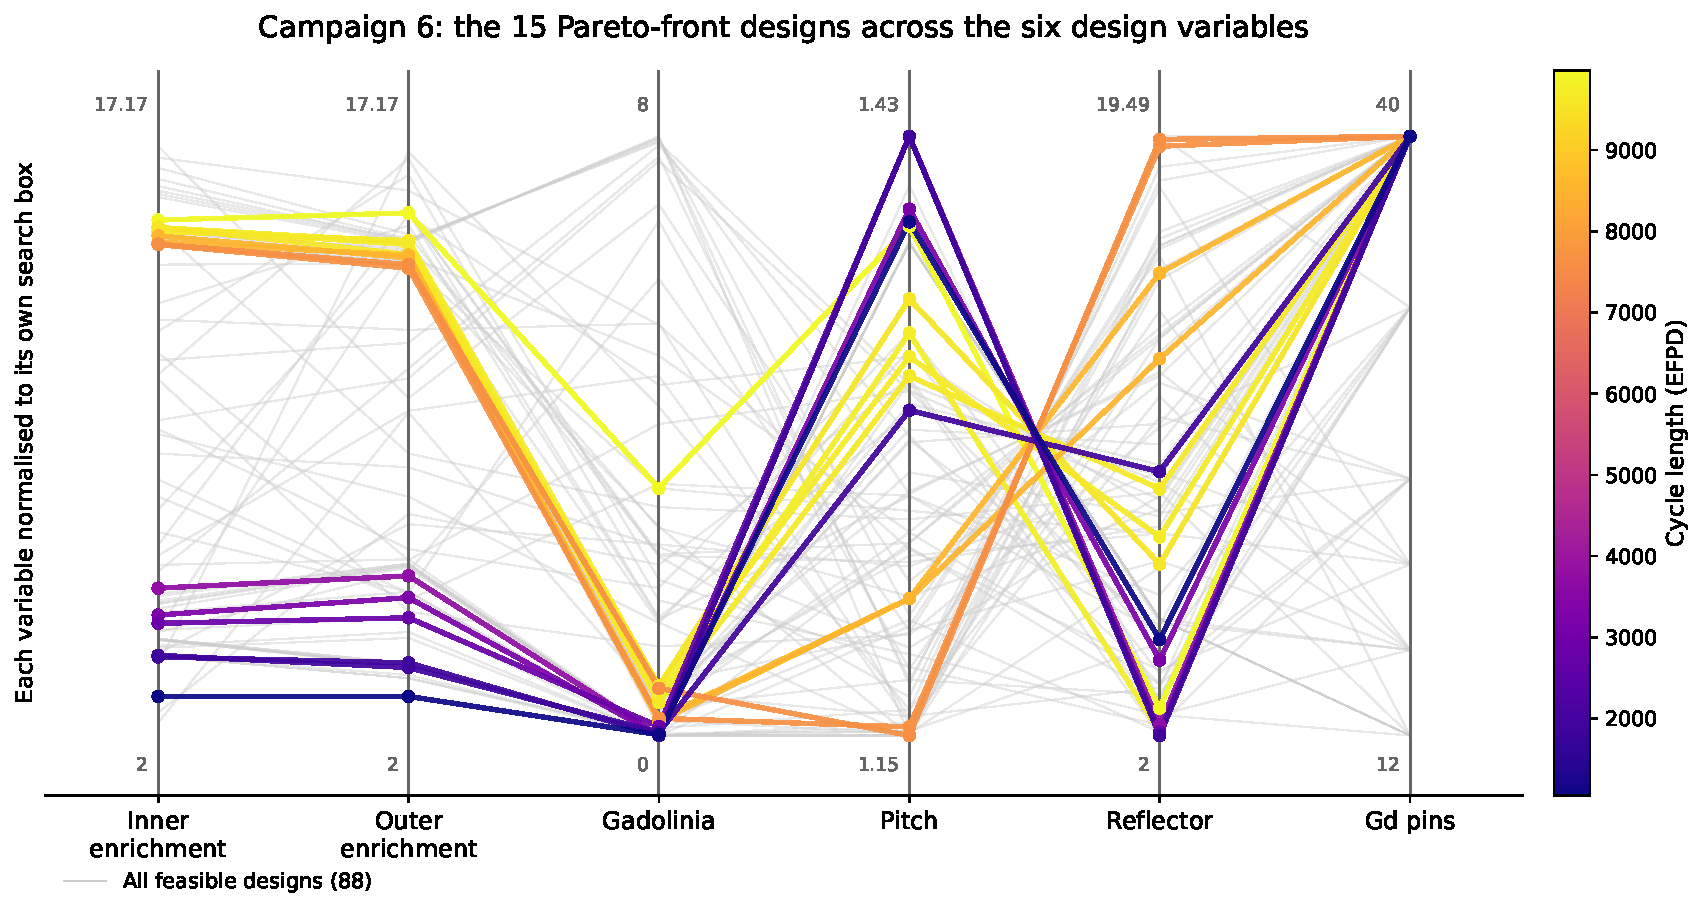
\includegraphics[width=\linewidth]{images/c6_vars_parallel}
  \caption{The fifteen Campaign 6 Pareto-front designs in parallel coordinates.}
  \label{fig:c6-parallel}
\end{figure}

The front is diverse in four of the six variables and unanimous in
one. The pitch spans its entire box, the reflector spans 99 per cent
of its box, the enrichments span about 80 per cent, and the gadolinia
content spans 0 to 3.30~wt\%. Every front design, without exception,
carries 40 gadolinium-bearing pins, the maximum of the ladder,
selected from a design of experiments that sampled all six ladder
values. The trade the optimiser found is many pins at low
concentration rather than few pins at high concentration. The archive
contains the concentrated alternative, a design at 7.92~wt\% in 16
pins reaching \num{9625} effective full power days, and it is
dominated by the dilute champion by \num{50} days and 0.006 in
peaking.

The preference for many dilute pins follows from the self-shielding
of the absorber. A poisoned pellet is optically black to thermal
neutrons, so absorption proceeds from its surface inward and the rate
at which the poison burns out is set by the surface exposed rather
than by the mass loaded (Section~\ref{sec:bg-gd}). Forty pins at low
concentration expose more surface than sixteen at high concentration,
so they burn out early and little absorber survives to the end of
cycle, whereas concentrated pins burn out late and carry a larger
residual penalty. The mechanism is self-shielding: the gadolinium atoms
in the outer layer of a pellet transmute faster than those
inside~\cite{gd_enriched_2021}. The early burnout has a cost
that this campaign did not score: it releases the hold-down before the
fuel has depleted and produces the reactivity hump analysed in
Section~\ref{sec:res-c9-gd}. Concentrated pins also depress their
own power more deeply, which loads their neighbours and raises the
peaking, in the direction that the 0.006 difference records.

The parallel-coordinates view also shows the vessel-fit coupling
directly. The long-cycle designs pair narrow pitch with a thick
reflector or wide pitch with a thin one, crossing between the two
axes, which is Equation~\eqref{eq:renv} acting as the budget it is.

\subsection{Variable influence and constraint activity}
\label{sec:res-c6-influence}

Figure~\ref{fig:c6-influence} shows the influence of each design variable
on the cycle length over the archive, coloured by the zoned-core peaking
factor and with the Pareto-front designs ringed. Each panel reports the
Spearman rank correlation of the variable with both objectives over the
feasible designs, and Table~\ref{tab:c6-spearman} collects the same
correlations.

\begin{figure}[htbp]
  \centering
  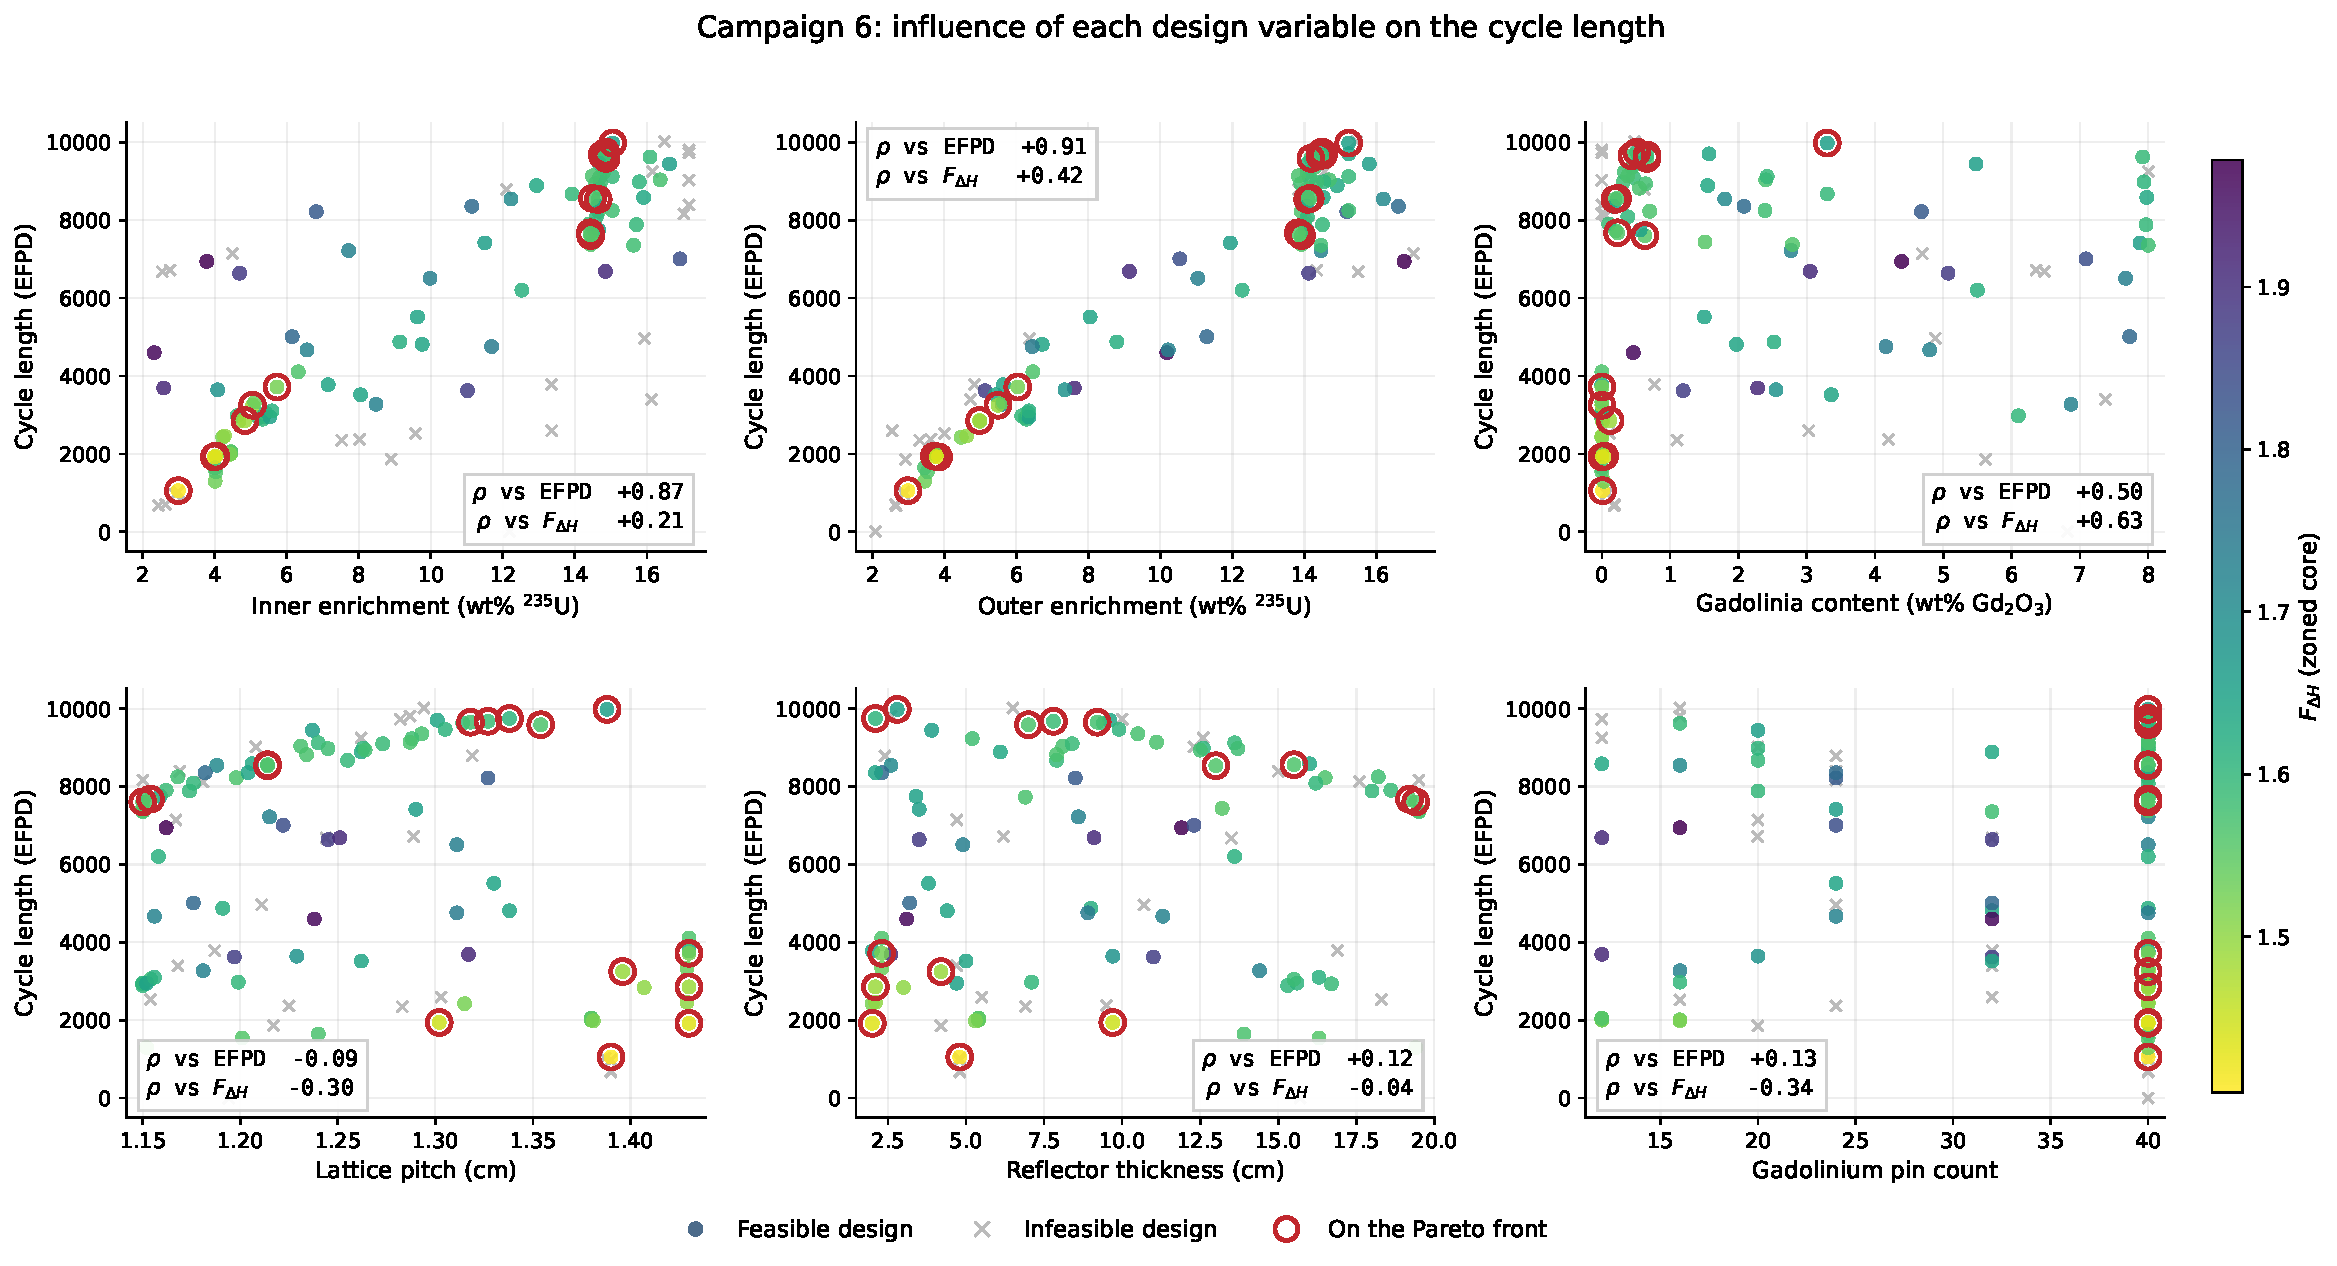
\includegraphics[width=\linewidth]{images/c6_vars_influence}
  \caption{Influence of each design variable on the cycle length over the Campaign 6 archive.}
  \label{fig:c6-influence}
\end{figure}

\begin{table}[htbp]
  \centering
  \caption{Spearman rank correlation of each design variable with the
  two objectives, over the 88 feasible designs of Campaign 6.}
  \label{tab:c6-spearman}
  \begin{tabular}{lcc}
    \toprule
    Variable & vs cycle length & vs $F_{\Delta H}$ \\
    \midrule
    $e_\mathrm{out}$  & $+0.905$ & $+0.422$ \\
    $e_\mathrm{in}$   & $+0.866$ & $+0.209$ \\
    gd                & $+0.498$ & $+0.633$ \\
    $n_\mathrm{Gd}$   & $+0.132$ & $-0.345$ \\
    $t_\mathrm{refl}$ & $+0.122$ & $-0.044$ \\
    $p$               & $-0.088$ & $-0.301$ \\
    \bottomrule
  \end{tabular}
\end{table}

Three readings are supported. First, enrichment dominates the cycle
length and nothing else approaches it, with the outer zone the
stronger of the two, consistent with the peripheral weighting of the
zoned map. Second, the gadolinia content correlates positively with
both objectives at once, which is not a physical benefit of the
absorber but a constraint-induced coupling. The absorber is present
only where the enrichment is high, because only there does the
reactivity ceiling demand it, so its apparent association with long
cycles is inherited from the enrichment. Third, the pitch and the
reflector barely move the cycle length while both act on the peaking,
which matches their role as radial-budget variables under the
vessel-fit coupling rather than as reactivity variables.

The reflector keeps that role in Campaign 8. With the pitch
fixed and the reflector capped at \SI{5.66}{cm}, the leakage-corrected
reactivity target moves by only about \SI{200}{pcm} over the whole
reflector range (Section~\ref{sec:meth-lax}), so in Campaign 8 the
reflector thickness acts on the radial power shape alone.

Figure~\ref{fig:c6-constraints} shows the reactivity constraint activity
across the archive.

\begin{figure}[htbp]
  \centering
  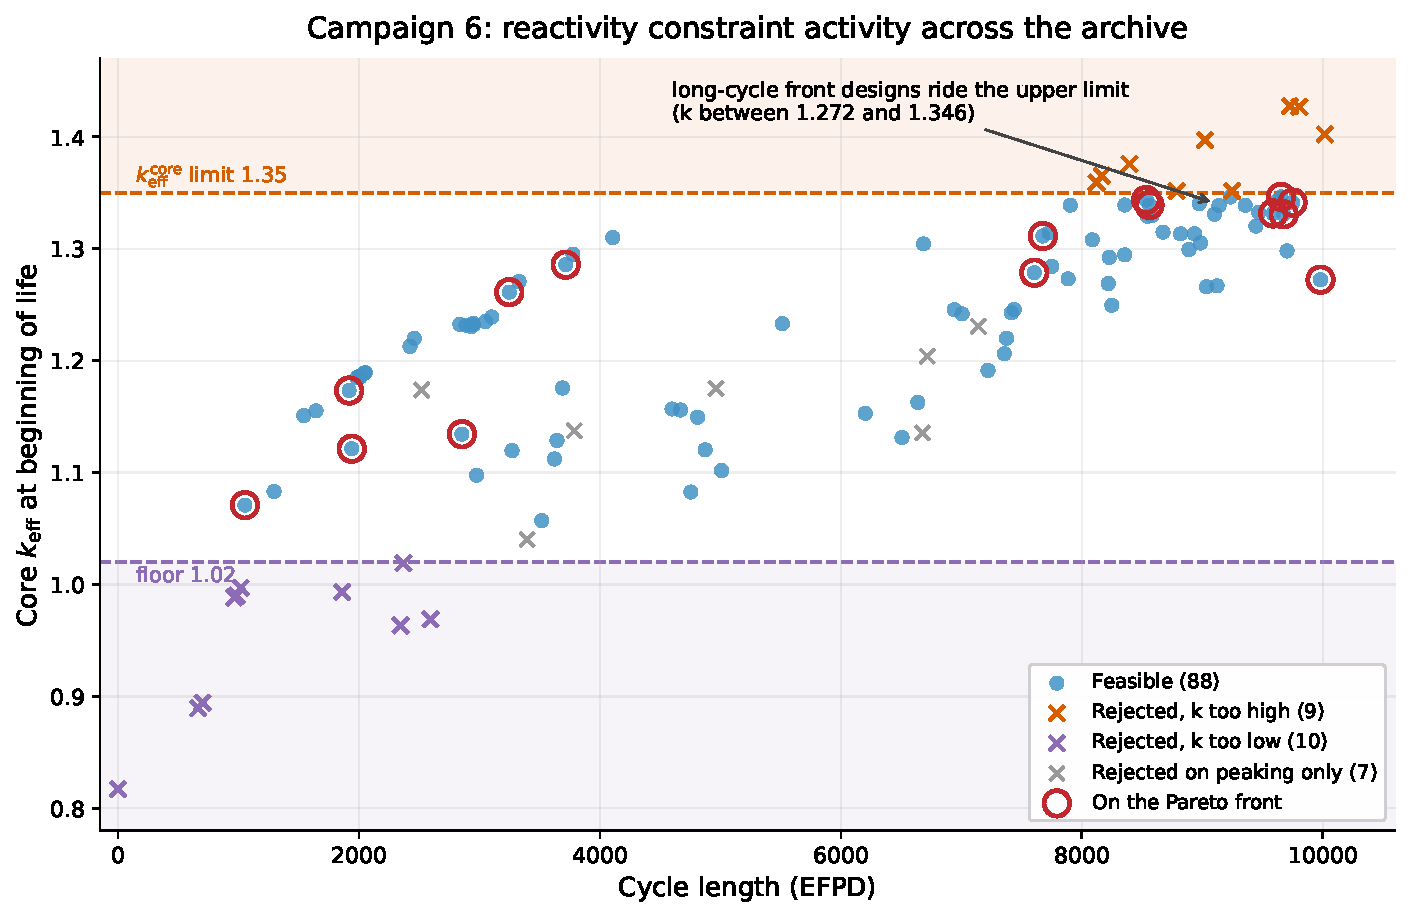
\includegraphics[width=0.92\linewidth]{images/c6_extra_constraints}
  \caption{Reactivity constraint activity across the Campaign 6 archive.}
  \label{fig:c6-constraints}
\end{figure}

The constraint activity closes the argument. Of the 26 rejections,
nine exceed the reactivity ceiling, ten fall below the floor of 1.02 as
genuinely subcritical or barely critical cores, and seven fail the
peaking limit alone. The long-cycle end of the front rides
the ceiling, with the nine designs beyond \num{7000} effective full
power days holding $k_\mathrm{eff}^\mathrm{core}$ between 1.272 and
1.346. The upper reactivity bound, not the peaking limit and not the
enrichment cap, is the active constraint that terminates the front on
the long-cycle side.

\subsection{The discharge-burnup screen}
\label{sec:res-c6-bscreen}

The depletion horizon of \SI{100}{\mega\watt\day\per\kilo\gram} is a
numerical device, and the discharge-qualification screen remains
$B_\mathrm{ATF} = \SI{75}{\mega\watt\day\per\kilo\gram}$, applied here
at candidate selection as Section~\ref{sec:meth-atf} prescribes.

The screen is consequential. Of the 88 feasible designs, 51 satisfy
it, and the nine long-cycle front designs beyond \num{7677} effective
full power days all exceed it, at end-of-cycle burnups between 75.9
and \SI{99.6}{\mega\watt\day\per\kilo\gram}. The screened front
therefore differs from the unscreened one at the long-cycle end, as
Table~\ref{tab:c6-front-screened} shows.

\begin{table}[htbp]
  \centering
  \caption{The Pareto front of the feasible designs satisfying the
  discharge-qualification screen
  $B_\mathrm{EOC} \le \SI{75}{\mega\watt\day\per\kilo\gram}$.}
  \label{tab:c6-front-screened}
  \begin{tabular}{cccccc}
    \toprule
    Index & EFPD & $F_{\Delta H}$ & $k_\mathrm{eff}^\mathrm{core}$ &
    $B_\mathrm{EOC}$ (MWd/kg) & gd (wt\%) \\
    \midrule
    101 & 7439 & 1.5564 & 1.24564 & 74.3 & 1.51 \\
     91 & 3717 & 1.5241 & 1.28575 & 37.1 & 0.00 \\
     85 & 3248 & 1.4938 & 1.26117 & 32.4 & 0.00 \\
    110 & 2855 & 1.4894 & 1.13427 & 28.5 & 0.12 \\
     69 & 1941 & 1.4480 & 1.12128 & 19.4 & 0.04 \\
    107 & 1919 & 1.4317 & 1.17329 & 19.2 & 0.00 \\
     59 & 1054 & 1.4041 & 1.07087 & 10.5 & 0.01 \\
    \bottomrule
  \end{tabular}
\end{table}

Under the screen the champion is design 101, at \num{7439} effective
full power days, $F_{\Delta H} = 1.5564$ and an end-of-cycle burnup of
\SI{74.3}{\mega\watt\day\per\kilo\gram}, which uses 99 per cent of the
qualification allowance. Its pitch of \SI{1.150}{cm} places it in the
guide-tube band of Section~\ref{sec:res-c7-limits}, so its peaking
value is qualified. The unscreened long-cycle designs, including
design 94, are conditional results. They quantify what the design
space offers if discharge burnups beyond
\SI{75}{\mega\watt\day\per\kilo\gram} can be qualified, and they are
reported as such rather than as candidates.

Neither champion is carried forward. Campaign 7 showed that the
reactivity ceiling of this campaign is a proxy for a controllability
requirement that must be measured (Section~\ref{sec:res-c7-screens}),
and Campaign 8 rebuilt the design space on that finding. The Campaign
6 designs are therefore the resolved front of a superseded
formulation, and the candidate list of this work is that of
Section~\ref{sec:res-c8-limits}.

\subsection{Comparison with the earlier campaigns and residual
caveats}
\label{sec:res-c6-compare}

Against the core-level results of the earlier campaigns the
improvement is large, and it decomposes cleanly into a bookkeeping
part and a physical part.

\begin{enumerate}
  \item In the Campaign 3 core validation, zero of 36 designs
        satisfied the peaking limit and the minimum core value was
        $2.013 \pm 0.018$. In Campaign 5 the closest approach was
        2.0012. In Campaign 6 the feasible median is 1.59 and the
        front reaches 1.4041.

  \item The reactivity basis change and the raised horizon are
        bookkeeping. The Campaign 5 re-scoring of
        Section~\ref{sec:res-c5-kbasis} quantifies the basis change
        in isolation, and the horizon acts only on censoring.

  \item The peaking collapse is attributable to the zoning alone,
        because $F_{\Delta H}$ is a beginning-of-life quantity that
        neither bookkeeping change can touch. The evaluator-zoned map
        of Section~\ref{sec:meth-zoning} is therefore the physically
        real driver of Campaign 6 feasibility.
\end{enumerate}

The enrichment landscape of the front is itself a result. The zoned
peripheral enrichments of the front span 3.4 to 17.5~wt\%, enclosing
the mid-single-digit values associated with first cores of this
reactor class and approaching, without being told to, the
low-enriched-uranium cap. The comparison with the reported refuelling
interval and the reported enrichment of the prototype is made once,
on the Campaign 8 front, in Section~\ref{sec:res-c8-mission}.

Campaign 7 and the axial study then showed that the high-enrichment end
of this front is not controllable by the regulating banks. Design 86,
at 14.4~wt\% in the volume-weighted sense, remains supercritical with
all regulating banks inserted in two and in three dimensions
(Section~\ref{sec:meth-lax}). The enrichment cap of the final campaign
is therefore a consequence of the control screen and not of the
low-enriched-uranium limit.

Five caveats bound the claims of this section.

\begin{enumerate}
  \item Every Campaign 6 cycle length is an exploration-tier value at
        the $4\,000\times60$ depletion fidelity of
        Table~\ref{tab:fidelity}, and is not directly comparable with
        the Campaign 3 to 5 values at $16\,000\times120$. The
        finalists are not re-scored, for the reason given in
        Section~\ref{sec:res-c6-bscreen}. Feasibility and every
        peaking value are unaffected, because the core solve is at
        full fidelity throughout.

  \item Every Campaign 6 cycle length is a two-dimensional value. The
        axial study of Section~\ref{sec:meth-lax}, performed on six
        designs of this campaign, measured the axial leakage factor at
        \num{1.0282} to \num{1.0298}, about \SI{3000}{pcm}, which at
        the end-of-cycle reactivity slopes of these designs is roughly
        450 to 500 effective full power days. The cycle lengths of
        Table~\ref{tab:c6-front} are overstated by that amount
        relative to a finite-height core, uniformly, so the ordering
        of the front is unaffected.

  \item Four front designs and the discharge-screen champion lie in
        the guide-tube band below \SI{1.2242}{cm}
        (Section~\ref{sec:res-c6-front}).

  \item The Campaign 6 depletion runs under the corrected restart
        configuration of Section~\ref{sec:restart_defect}, verified in
        the campaign metadata, so its burnups are free of the defect
        that affected Campaigns 3 to 5.

  \item The frozen hypervolume reference was constructed from a
        two-design front and proved blind to the entire short-cycle
        half of the trade. The convergence claim of this campaign
        therefore rests on the frozen metric, the full-range metric,
        the relaxation cascade and the margin-feasible count jointly,
        and Figure~\ref{fig:c6-convergence} reports the first two side
        by side. Reporting a single hypervolume number against a
        single reference is, on this evidence, not a sufficient
        convergence statement for a front whose extent is unknown in
        advance~\cite{zitzler_2003_performance}.
\end{enumerate}

What carries forward from this campaign is its architecture rather
than its designs. The four-part acquisition of
Section~\ref{sec:meth-acq}, the surrogate search setting, the two
health indicators of the stopping rule, the core-basis reactivity
window and the evaluator-level zoning are all retained by Campaigns 7
and 8. The designs themselves are superseded, first by the measured
controllability screen and then by the fixed-pitch design space.

\openpoint{Section~\ref{sec:res-c7-uncertainty} attributes to this
section an entropy study that bounded the systematic shift of the
core peaking factor at $\pm 0.02$. That study is not documented here.
Either insert its text into this section or redirect the reference to
where the study is reported.}

\section{Campaign 7: the controllability screen}
\label{sec:res-c7}

Campaign 6 closed with a front whose long-cycle end rode the
reactivity ceiling, and with the observation that the ceiling of 1.35
proxied controllable excess reactivity without a rod model. Campaign 7
replaces the proxy by a measurement. Every evaluation now solves the
beginning-of-life core a second time with the sixteen regulating-bank
control rod assemblies inserted, and the resulting eigenvalue enters the
constraint set directly. The campaign ran 60 evaluations on the AWS
instance in \SI{15.82}{h}, and every one of them completed without
error.

\subsection{The one change and its two consequences}
\label{sec:res-c7-basis}

The constraint added is the controllability screen of
Section~\ref{sec:meth-ctrl}.

\begin{equation}
g_\mathrm{ctrl}(\mathbf{x}) = k_\mathrm{RE}(\mathbf{x}) - (1 - \Delta\rho_\mathrm{op}) \le 0
\label{eq:g-ctrl}
\end{equation}

\noindent where the symbols have the following meaning.

\begin{itemize}
  \item $k_\mathrm{RE}$ is the effective multiplication factor of the
        32-assembly core at beginning of life with the sixteen
        regulating-bank assemblies inserted and the sixteen
        shutdown-bank assemblies withdrawn, dimensionless. It is not
        the all-rods-in state of Section~\ref{sec:meth-ctrl}.

  \item $\Delta\rho_\mathrm{op}$ is the operating subcriticality margin
        demanded of the regulating banks, \num{0.01} in units of $k$,
        that is \SI{1000}{pcm}.

  \item $\mathbf{x}$ is the design vector.
\end{itemize}

Two settings changed with it. The reactivity ceiling was lowered from
1.35 to 1.126, a value derived before the campaign from the smallest
regulating-bank worth measured on eight Campaign 6 designs, and the
enrichment cap was lowered to \SI{12}{wt\%} on the as-built peripheral
ring, giving a search box of 3.0 to \SI{10.43}{wt\%}. Both were
intended as consequences of the controllability requirement rather than
as independent changes, and the campaign tests whether they were
consistent with the measurement they were meant to anticipate.

\subsection{Design of experiments and the three infill blocks}
\label{sec:res-c7-blocks}

The campaign ran a design of experiments of 42 followed by three infill
blocks of six. Table~\ref{tab:c7-blocks} records the outcome of each
block and Figure~\ref{fig:c7-diversity} its diversity, measured as the
spread of each design variable within the block as a fraction of the
range spanned by the whole archive. In the table the hypervolume is the
frozen-reference value written at each block boundary, and the spread is
listed for the four non-geometric variables. Infill blocks 1 and 3 vary
only the pitch and the reflector thickness, and neither returned a
feasible design.

\begin{table}[htbp]
  \centering
  \caption{Campaign 7 blocks.}
  \label{tab:c7-blocks}
  \begin{tabular}{lccll}
    \toprule
    Block & Designs & Feasible & Hypervolume & Spread in $e_\mathrm{in}$, $e_\mathrm{out}$, $w_\mathrm{Gd}$, $n_\mathrm{Gd}$ \\
    \midrule
    DOE      & 42 & 13 & 773.7 & 0.98 to 1.00 \\
    Infill 1 &  6 &  0 & 773.7 & 0.000 to 0.002 \\
    Infill 2 &  6 &  3 & 996.5 & 0.07 to 0.29 \\
    Infill 3 &  6 &  0 & 996.5 & 0.015 to 0.13 \\
    \bottomrule
  \end{tabular}
\end{table}

\begin{figure}[htbp]
  \centering
  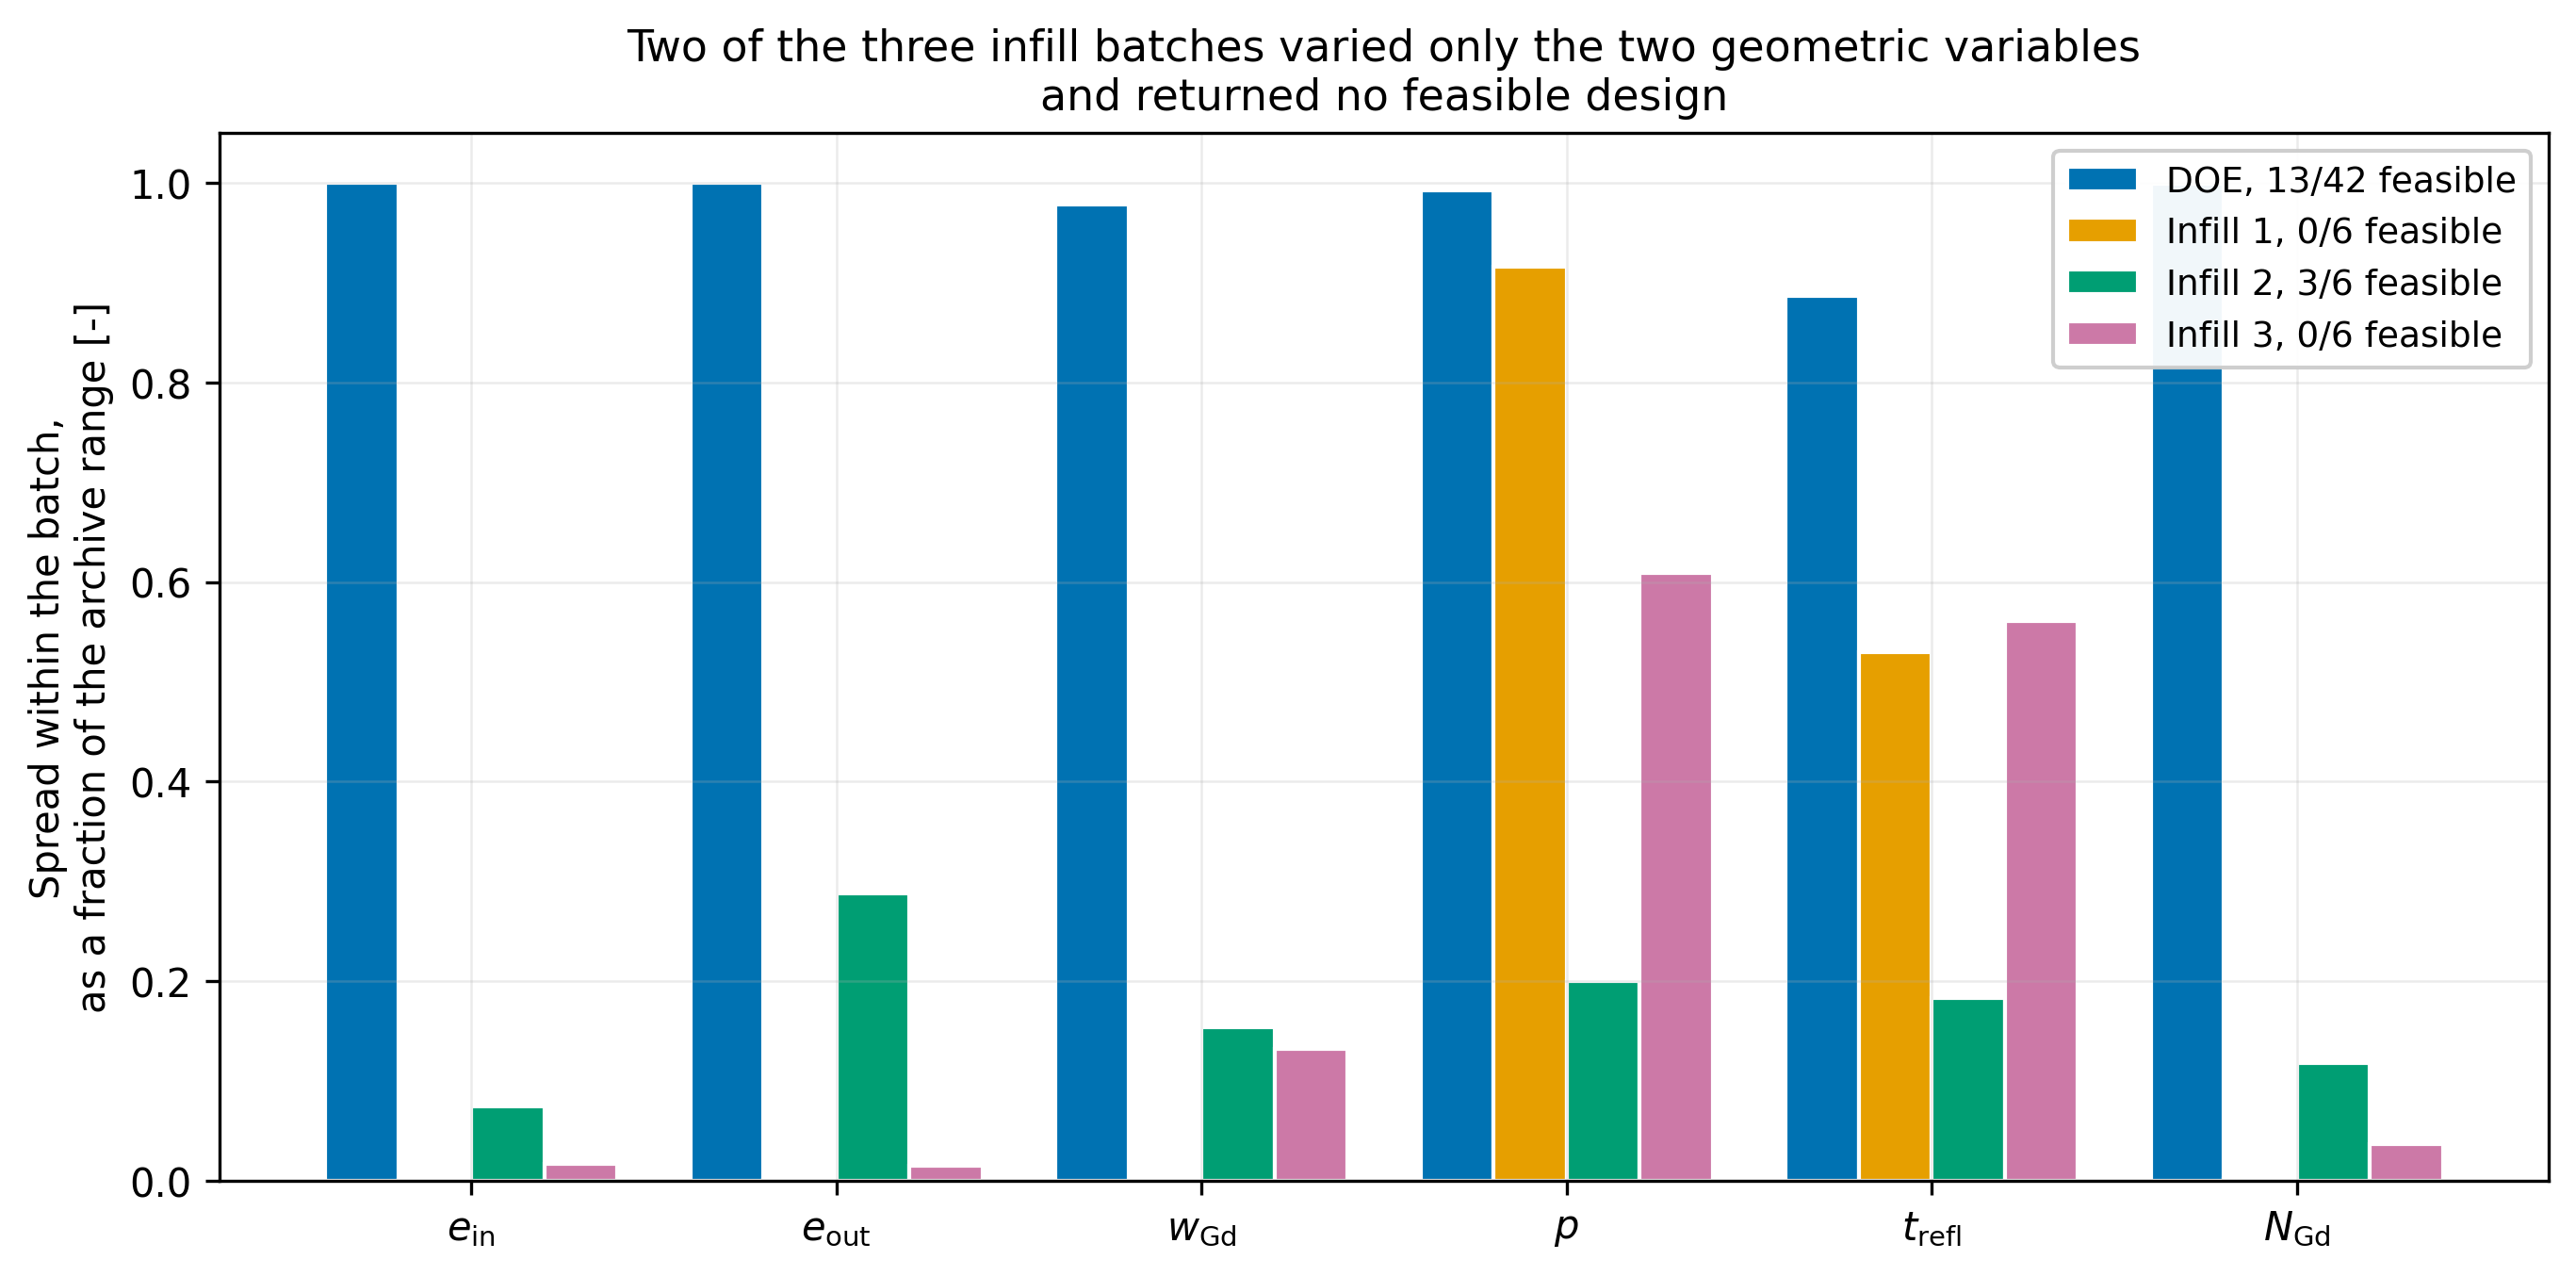
\includegraphics[width=\linewidth]{images/c7_infill_diversity}
  \caption{Within-block spread of each design variable in Campaign 7, as a fraction of the archive range.}
  \label{fig:c7-diversity}
\end{figure}

Two of the three infill blocks collapsed. In block 1 the six designs
share one enrichment pair, \num{5.09} and \SI{4.04}{wt\%}, exactly zero
gadolinia and 24 poisoned pins, and differ only in pitch and reflector
thickness. In block 3 the same pattern recurs at \num{8.13} and
\SI{7.33}{wt\%} with 32 pins. All twelve designs of the two blocks
failed the reactivity ceiling.

The cause is a configuration regression, not a new defect. The
acquisition ran with a minimum separation of 0.05 and a feasibility
margin of 1.0 standard deviation, the default values of the launcher,
where Campaign 6 had established 0.14 and 1.5 in
Section~\ref{sec:res-c6-margin}. The two collapsed blocks satisfied the
separation rule as coded, with pairwise separations of 0.059 to 0.089,
because the rule averages over all six variables and two of them
supplied the whole distance. A per-variable minimum spread would have
rejected both batches.

The consequence for the convergence record is that the flat
hypervolume of block 3 is not a stopping signal. Under the Campaign 6
rule a zero gain counts toward stopping only when the acquisition is
functioning, and block 3 demonstrably was not. The campaign therefore
ends with an unconverged front, and its value lies in the constraint
measurements rather than in the front itself.

\subsection{Feasibility and the nesting of the two screens}
\label{sec:res-c7-screens}

Of the 60 designs, 16 are feasible against all six constraints, a
fraction of \SI{26.7}{\%} against \SI{67}{\%} in the Campaign 6 design
of experiments. Table~\ref{tab:c7-nesting} gives the constraint census,
and Figure~\ref{fig:c7-screens} shows the two reactivity screens in the
plane of the unrodded and the rodded core eigenvalues, with the fourteen
designs rejected only by the derived ceiling marked by open circles.
No design fails the enrichment or the geometric constraint, two fail
the peaking limit, nine fall below the reactivity floor, 34 exceed the
ceiling and 20 fail the controllability screen.

\begin{table}[htbp]
  \centering
  \caption{Constraint census of Campaign 7 and the joint activity of the two reactivity screens.}
  \label{tab:c7-nesting}
  \begin{tabular}{lc}
    \toprule
    Outcome & Designs \\
    \midrule
    Fail $g_{k\max}$ at 1.126                      & 34 \\
    Fail $g_\mathrm{ctrl}$                         & 20 \\
    Fail $g_\mathrm{ctrl}$ and pass $g_{k\max}$    &  0 \\
    Fail $g_{k\max}$ and pass $g_\mathrm{ctrl}$    & 14 \\
    Pass every constraint except $g_{k\max}$       & 14 \\
    Feasible on all six                            & 16 \\
    \bottomrule
  \end{tabular}
\end{table}

\begin{figure}[htbp]
  \centering
  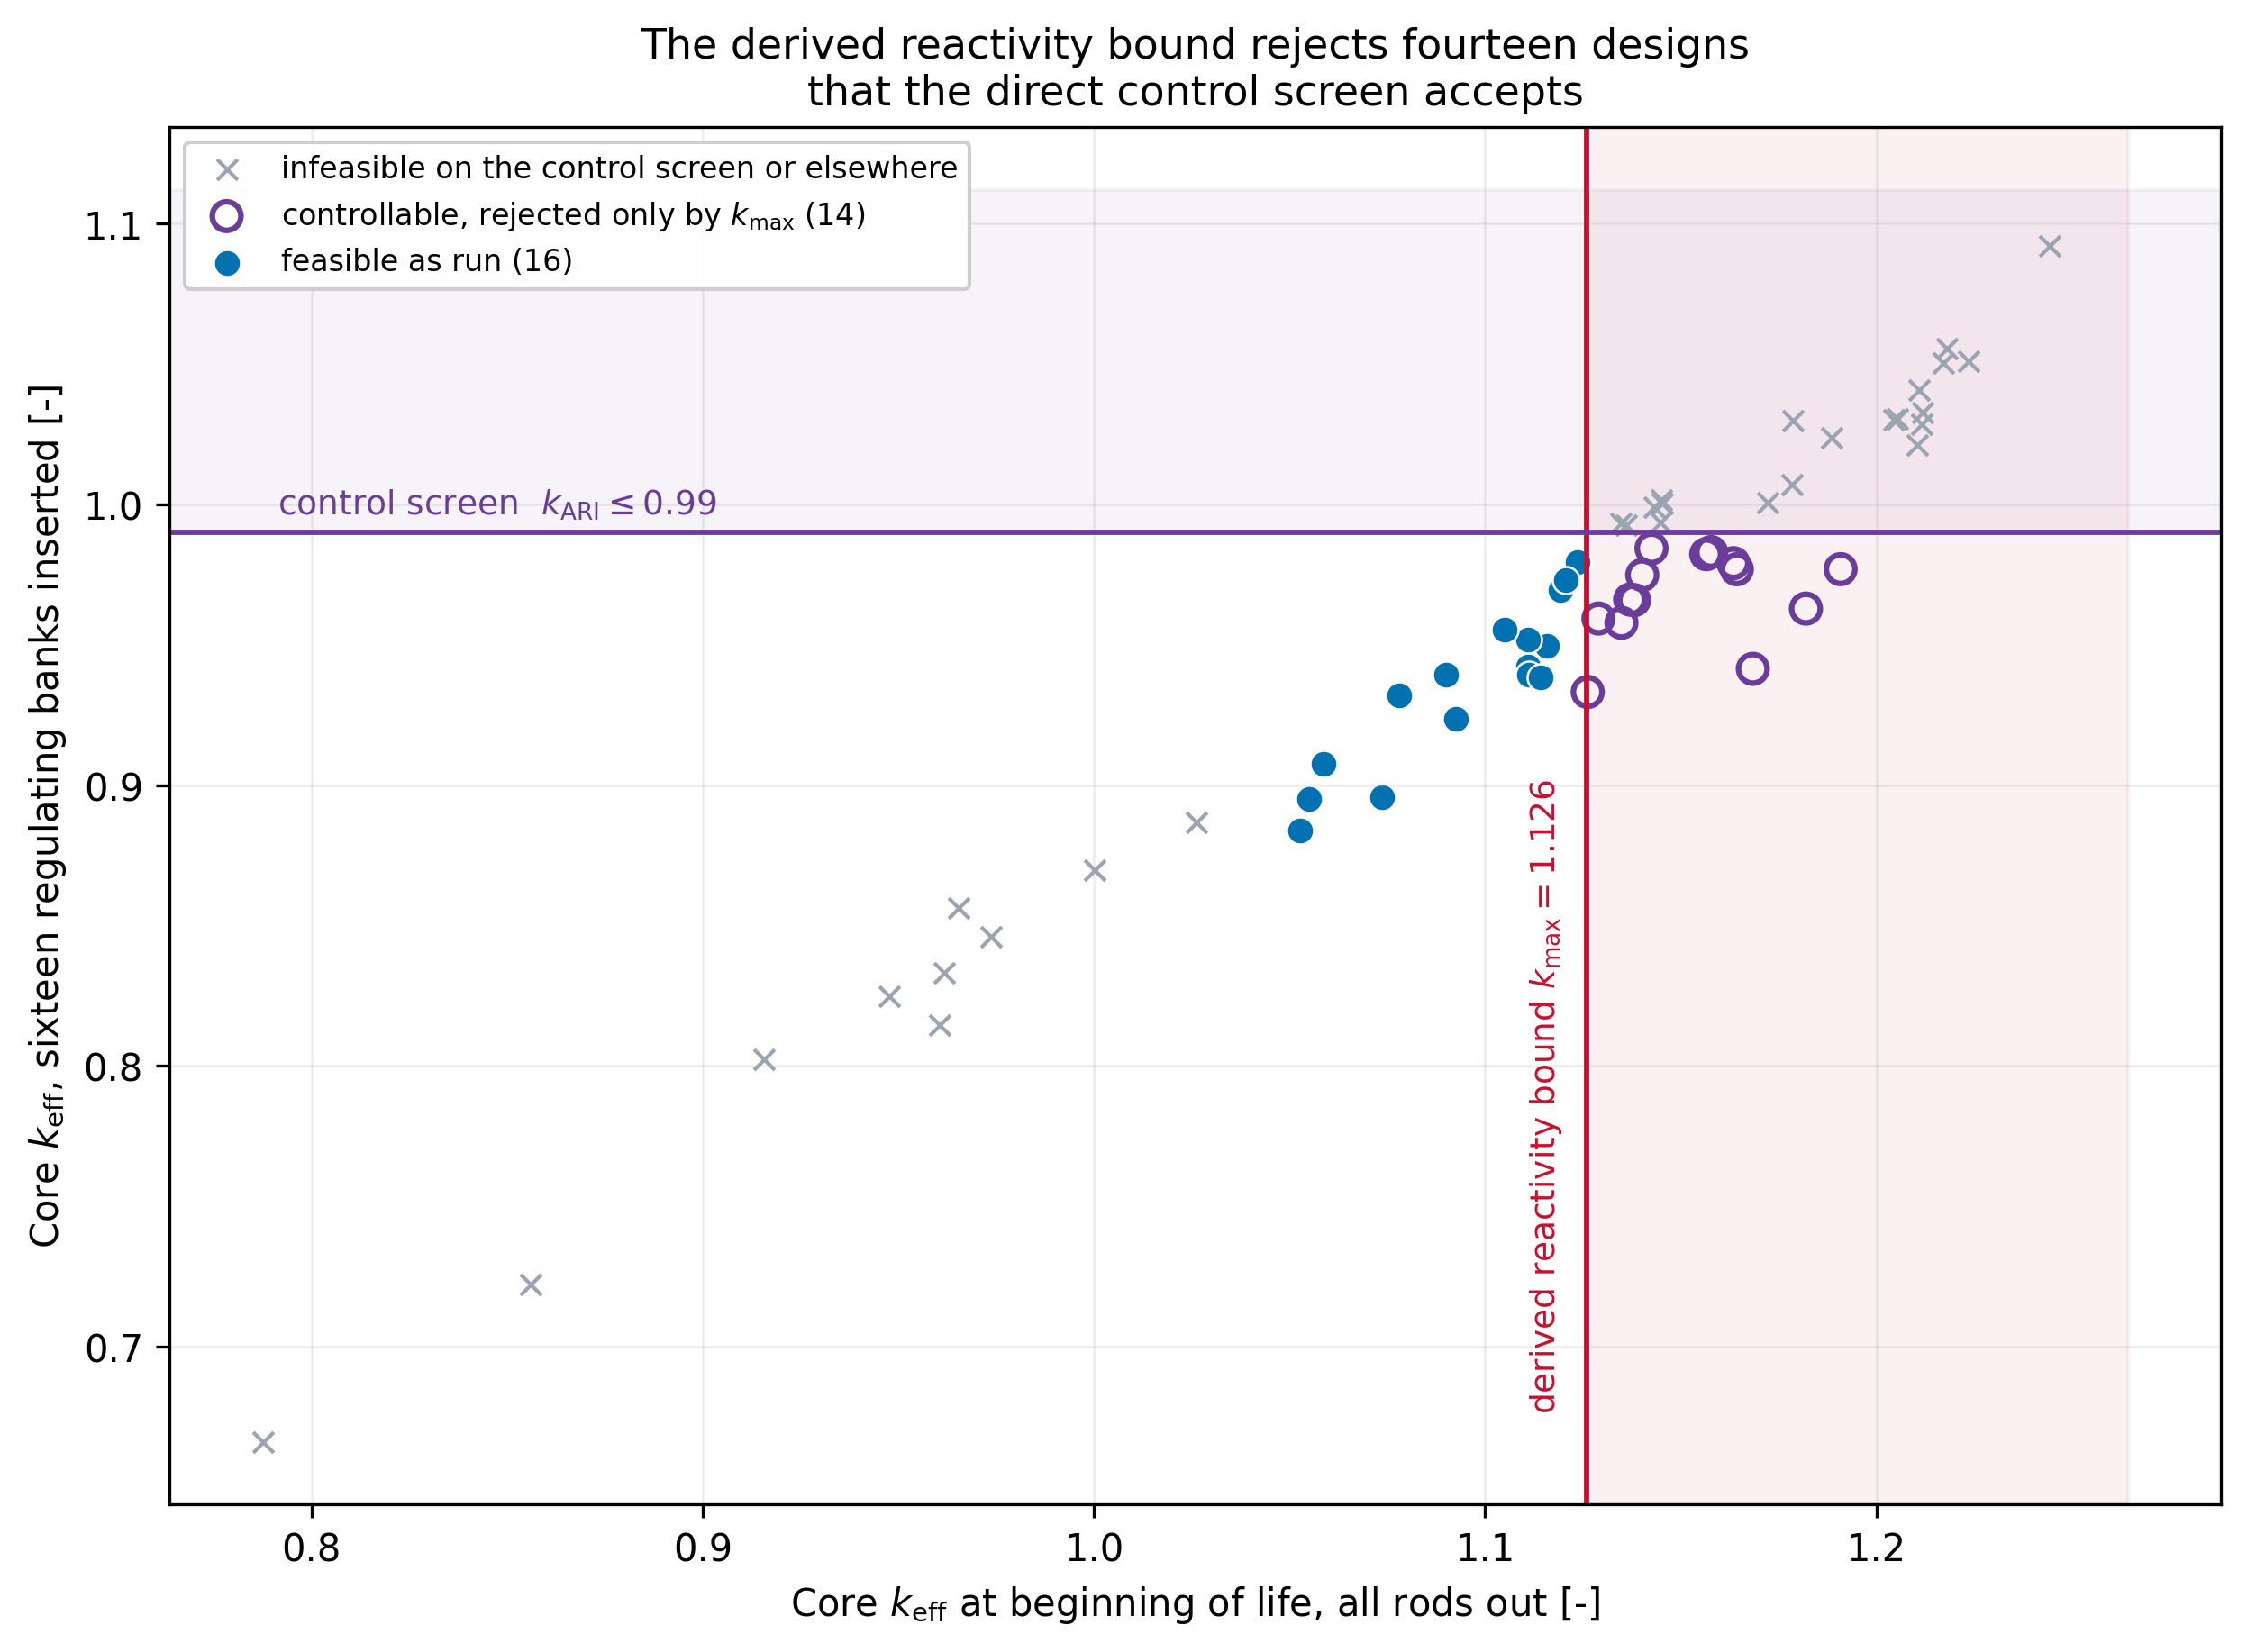
\includegraphics[width=0.9\linewidth]{images/c7_ctrl_screen}
  \caption{The two reactivity screens of Campaign 7 in the plane of the unrodded and the all-regulating-banks-in core eigenvalues.}
  \label{fig:c7-screens}
\end{figure}

The two screens are nested. Not one design in the archive fails the
control screen without also failing the derived ceiling, and fourteen
designs fail the ceiling while their own measured bank worth shows them
controllable at the stated margin. Figure~\ref{fig:c7-screens} shows
the nesting directly. The ceiling of 1.126 therefore did no work that
the measurement did not do, and it discarded fourteen evaluations that
the measurement would have kept.

The derivation explains why. The eight Campaign 6 designs from which
1.126 was obtained had worths between \num{12174} and
\SI{12718}{pcm}, a spread of four per cent. The 60 designs of this
campaign span \num{10936} to \SI{22699}{pcm}, a factor of two. Eight
near-identical designs under-sampled the variability by an order of
magnitude, and the resulting bound is at once too tight where it
matters and not conservative in general. Restricted to the 22 designs
with an unrodded eigenvalue between 1.09 and 1.17, the smallest
measured worth of \SI{14126}{pcm} implies a ceiling of 1.151, while the
smallest worth in the whole archive implies 1.110.

The front reflects the same fact. As run, the feasible non-dominated set
holds three designs, all from infill block 2. With the derived ceiling
removed and the measured control screen retained, the feasible set grows
from 16 to 30 designs, the front doubles to six, the peaking floor moves
from 1.565 to 1.525, and the hypervolume against the frozen reference
rises from 996.5 to 1054.1, a gain of \SI{5.8}{\%}. Three of the six
designs come from infill block 3, the block that under the ceiling
contributed nothing. Table~\ref{tab:c7-front} lists both fronts and
Figure~\ref{fig:c7-pareto} places them in the objective plane.
Designs 48, 53 and 49 form the front as run, and all six form it when the
measured control screen alone governs reactivity. The bank worth in the
table is the difference between the unrodded and the all-banks-in
eigenvalues. In the figure filled markers are feasible as run and open
circles are controllable designs rejected only by the derived ceiling.
The solid front is the one the campaign reported, and the dashed front is
the one the measured control screen supports.

\begin{table}[htbp]
  \centering
  \small
  \caption{The Campaign 7 front under the two screening rules.}
  \label{tab:c7-front}
  \begin{tabular}{ccccccccccc}
    \toprule
    Design & EFPD & $F_{\Delta H}$ & $e_\mathrm{in}$ & $e_\mathrm{out}$ & $w_\mathrm{Gd}$ & $p$ & $t_\mathrm{refl}$ & $n_\mathrm{Gd}$ & $k_\mathrm{eff}^\mathrm{core}$ & worth \\
           & [d] & [-] & [wt\%] & [wt\%] & [wt\%] & [cm] & [cm] & [-] & [-] & [pcm] \\
    \midrule
    59 & 3886 & 1.525 & 8.13 & 7.33 & 1.10 & 1.150 & 19.49 & 32 & 1.135 & 17699 \\
    57 & 4045 & 1.528 & 8.13 & 7.33 & 1.21 & 1.176 & 17.87 & 32 & 1.137 & 17094 \\
    55 & 4502 & 1.529 & 8.14 & 7.34 & 1.10 & 1.238 & 14.09 & 32 & 1.143 & 15815 \\
    48 & 4745 & 1.565 & 8.71 & 7.80 & 1.93 & 1.237 & 14.06 & 40 & 1.119 & 14970 \\
    53 & 4899 & 1.590 & 8.97 & 7.88 & 1.96 & 1.249 & 13.21 & 40 & 1.121 & 14734 \\
    49 & 5087 & 1.598 & 9.19 & 8.30 & 2.13 & 1.267 & 12.29 & 40 & 1.124 & 14416 \\
    \bottomrule
  \end{tabular}
\end{table}

\begin{figure}[htbp]
  \centering
  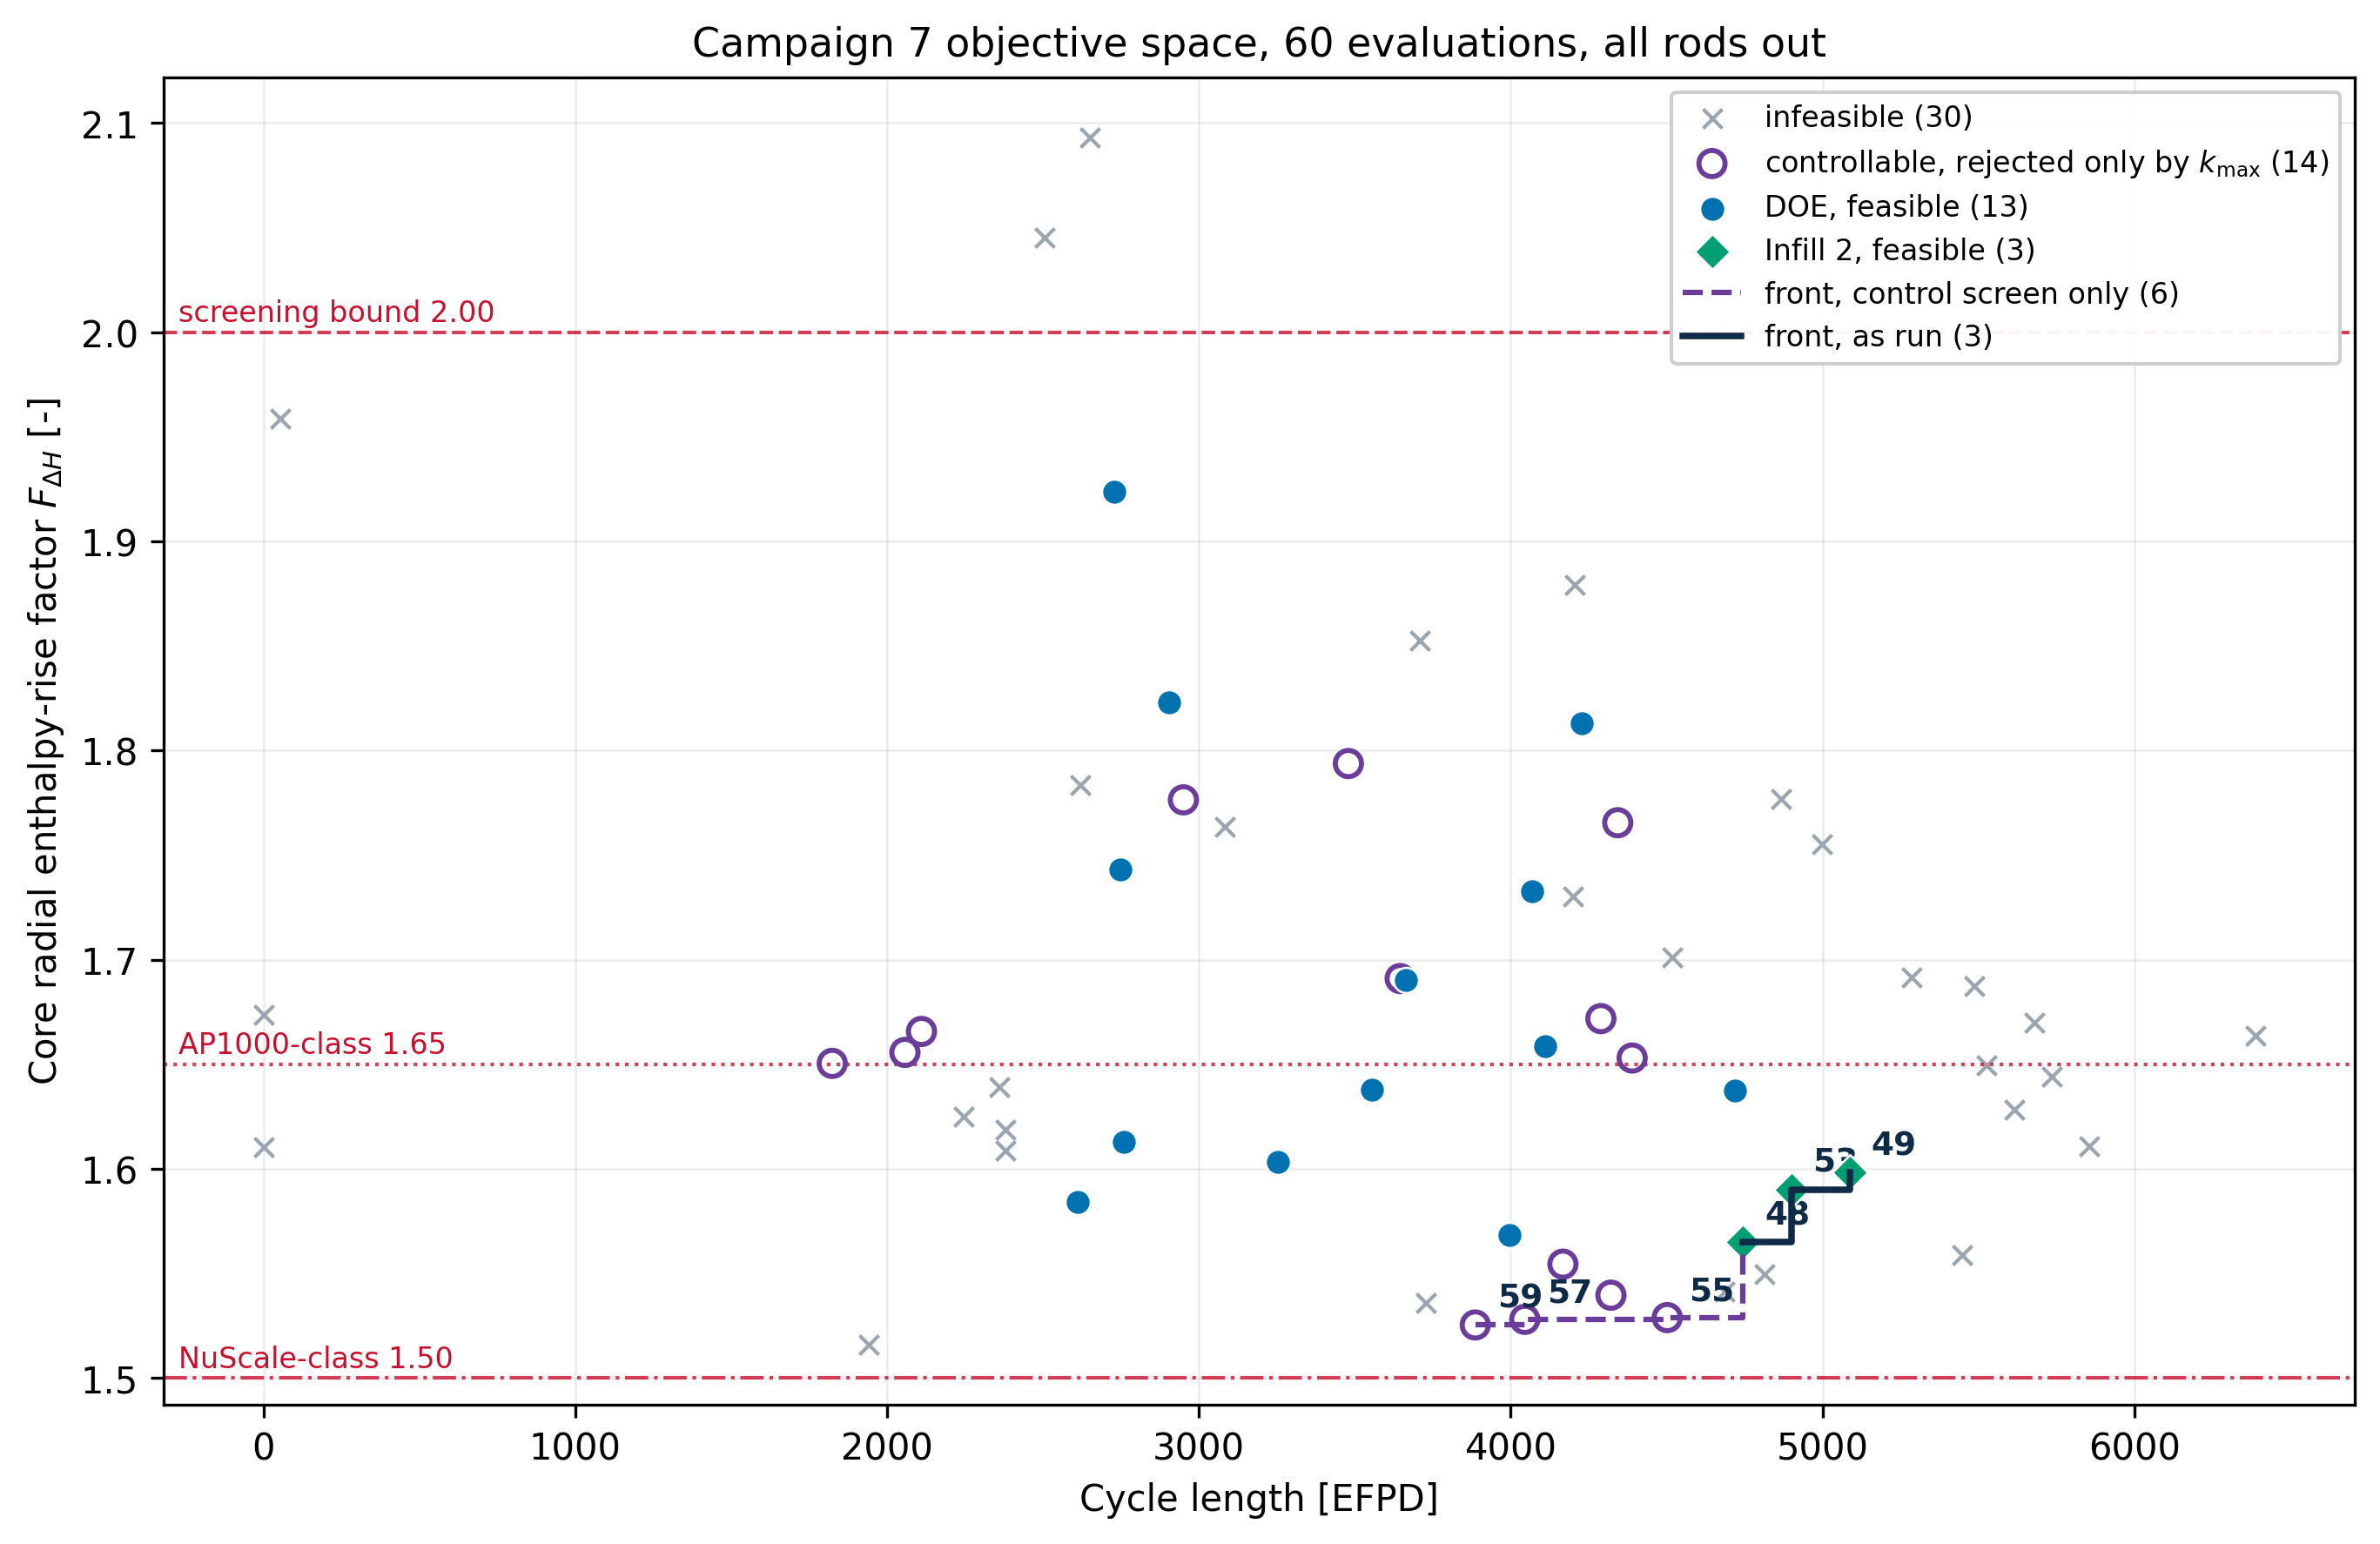
\includegraphics[width=\linewidth]{images/c7_pareto_60}
  \caption{Campaign 7 objective space with all rods out.}
  \label{fig:c7-pareto}
\end{figure}

Two properties of the front as run deserve stating. Its three designs
sit \num{240} to \SI{680}{pcm} below the ceiling, so the front is a
constraint boundary and not an interior trade. And the cycle lengths
are not comparable with Campaign 6, because the enrichment box is a
different one, and the longest feasible cycle of 5087 EFPD says nothing
about the reactor class that the 9981 EFPD of Campaign 6 did not
already say.

%% AUTHOR: one paragraph on why the low-peaking end of the control-screen
%% front lives at thick reflectors and narrow pitch, and on the physical
%% meaning of a front that doubles when a surrogate bound is removed.

\subsection{Regulating-bank worth and the reason the screens nest}
\label{sec:res-c7-worth}

The worth of the sixteen regulating banks is defined on the two core
solves of every evaluation.

\begin{equation}
\rho_\mathrm{bank}(\mathbf{x}) = k_\mathrm{eff}^\mathrm{core}(\mathbf{x}) - k_\mathrm{RE}(\mathbf{x})
\label{eq:bank-worth}
\end{equation}

\noindent where the symbols have the following meaning.

\begin{itemize}
  \item $\rho_\mathrm{bank}$ is the bank worth in units of $k$,
        dimensionless, reported in pcm by multiplying by $10^5$.

  \item $k_\mathrm{eff}^\mathrm{core}$ is the unrodded core eigenvalue
        at beginning of life, dimensionless.

  \item $k_\mathrm{RE}$ is the eigenvalue with the sixteen
        regulating-bank assemblies inserted, dimensionless.
\end{itemize}

Across the archive the worth ranges from \num{10936} to
\SI{22699}{pcm} with a median of \SI{16510}{pcm}. Figure~\ref{fig:c7-worth}
shows its two strongest drivers, with least-squares trends drawn as
visual guides only, and Figure~\ref{fig:c7-influence} the rank
correlations of all six variables with the objectives, the worth and the
rodded peaking, over the whole archive and over the feasible subset.

\begin{figure}[htbp]
  \centering
  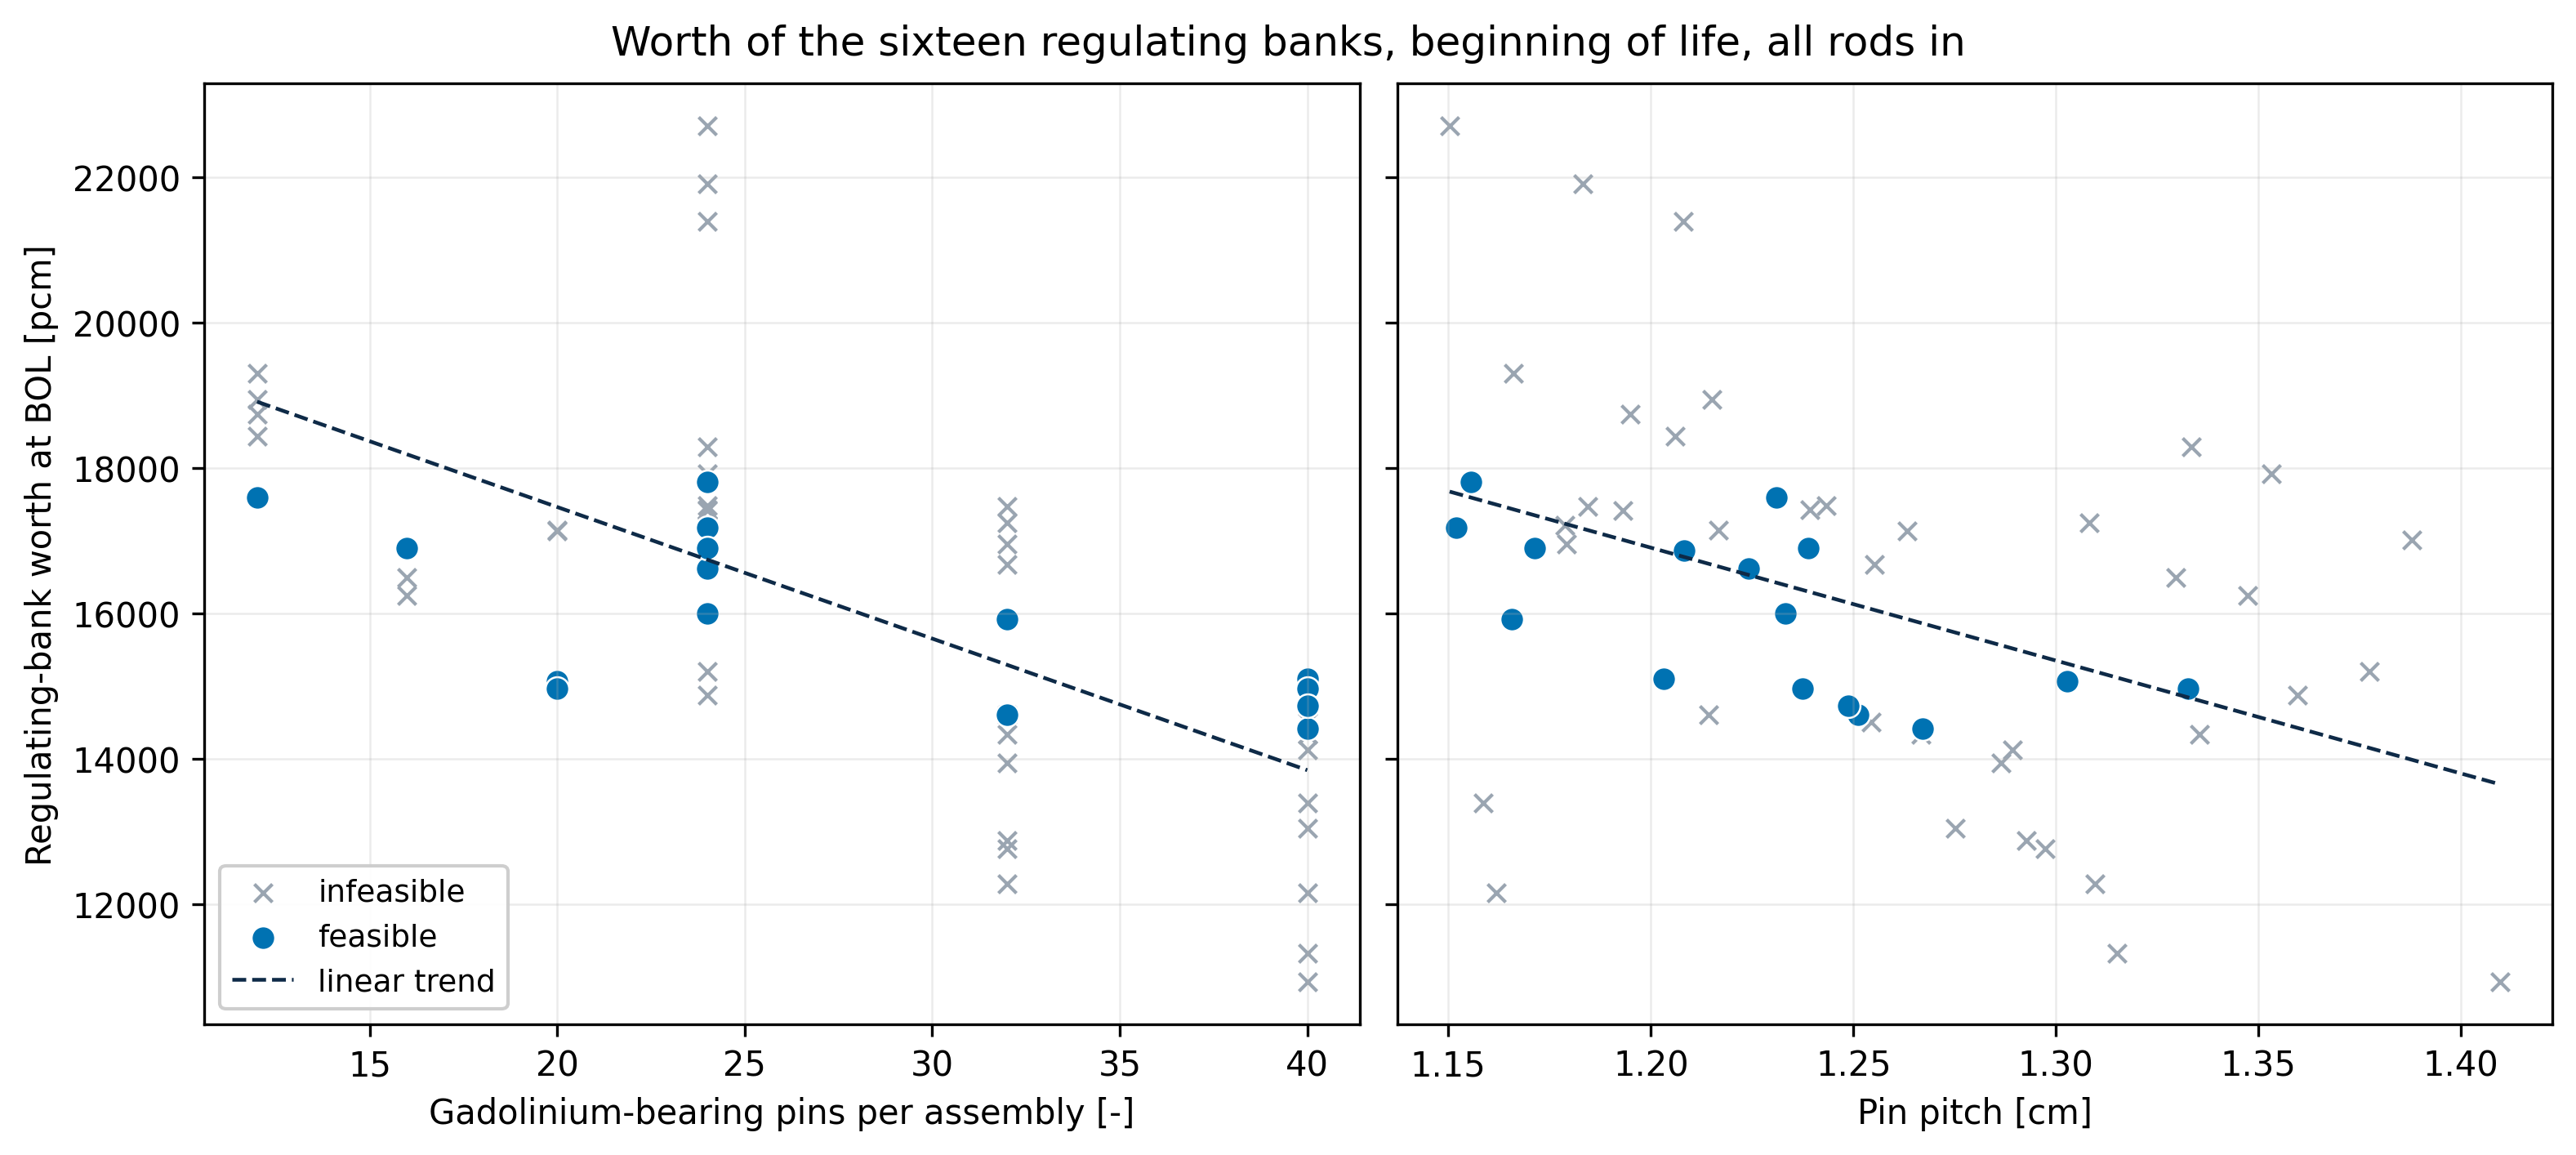
\includegraphics[width=\linewidth]{images/c7_rod_worth}
  \caption{Worth of the sixteen regulating banks against the gadolinium pin count and the pin pitch.}
  \label{fig:c7-worth}
\end{figure}

\begin{figure}[htbp]
  \centering
  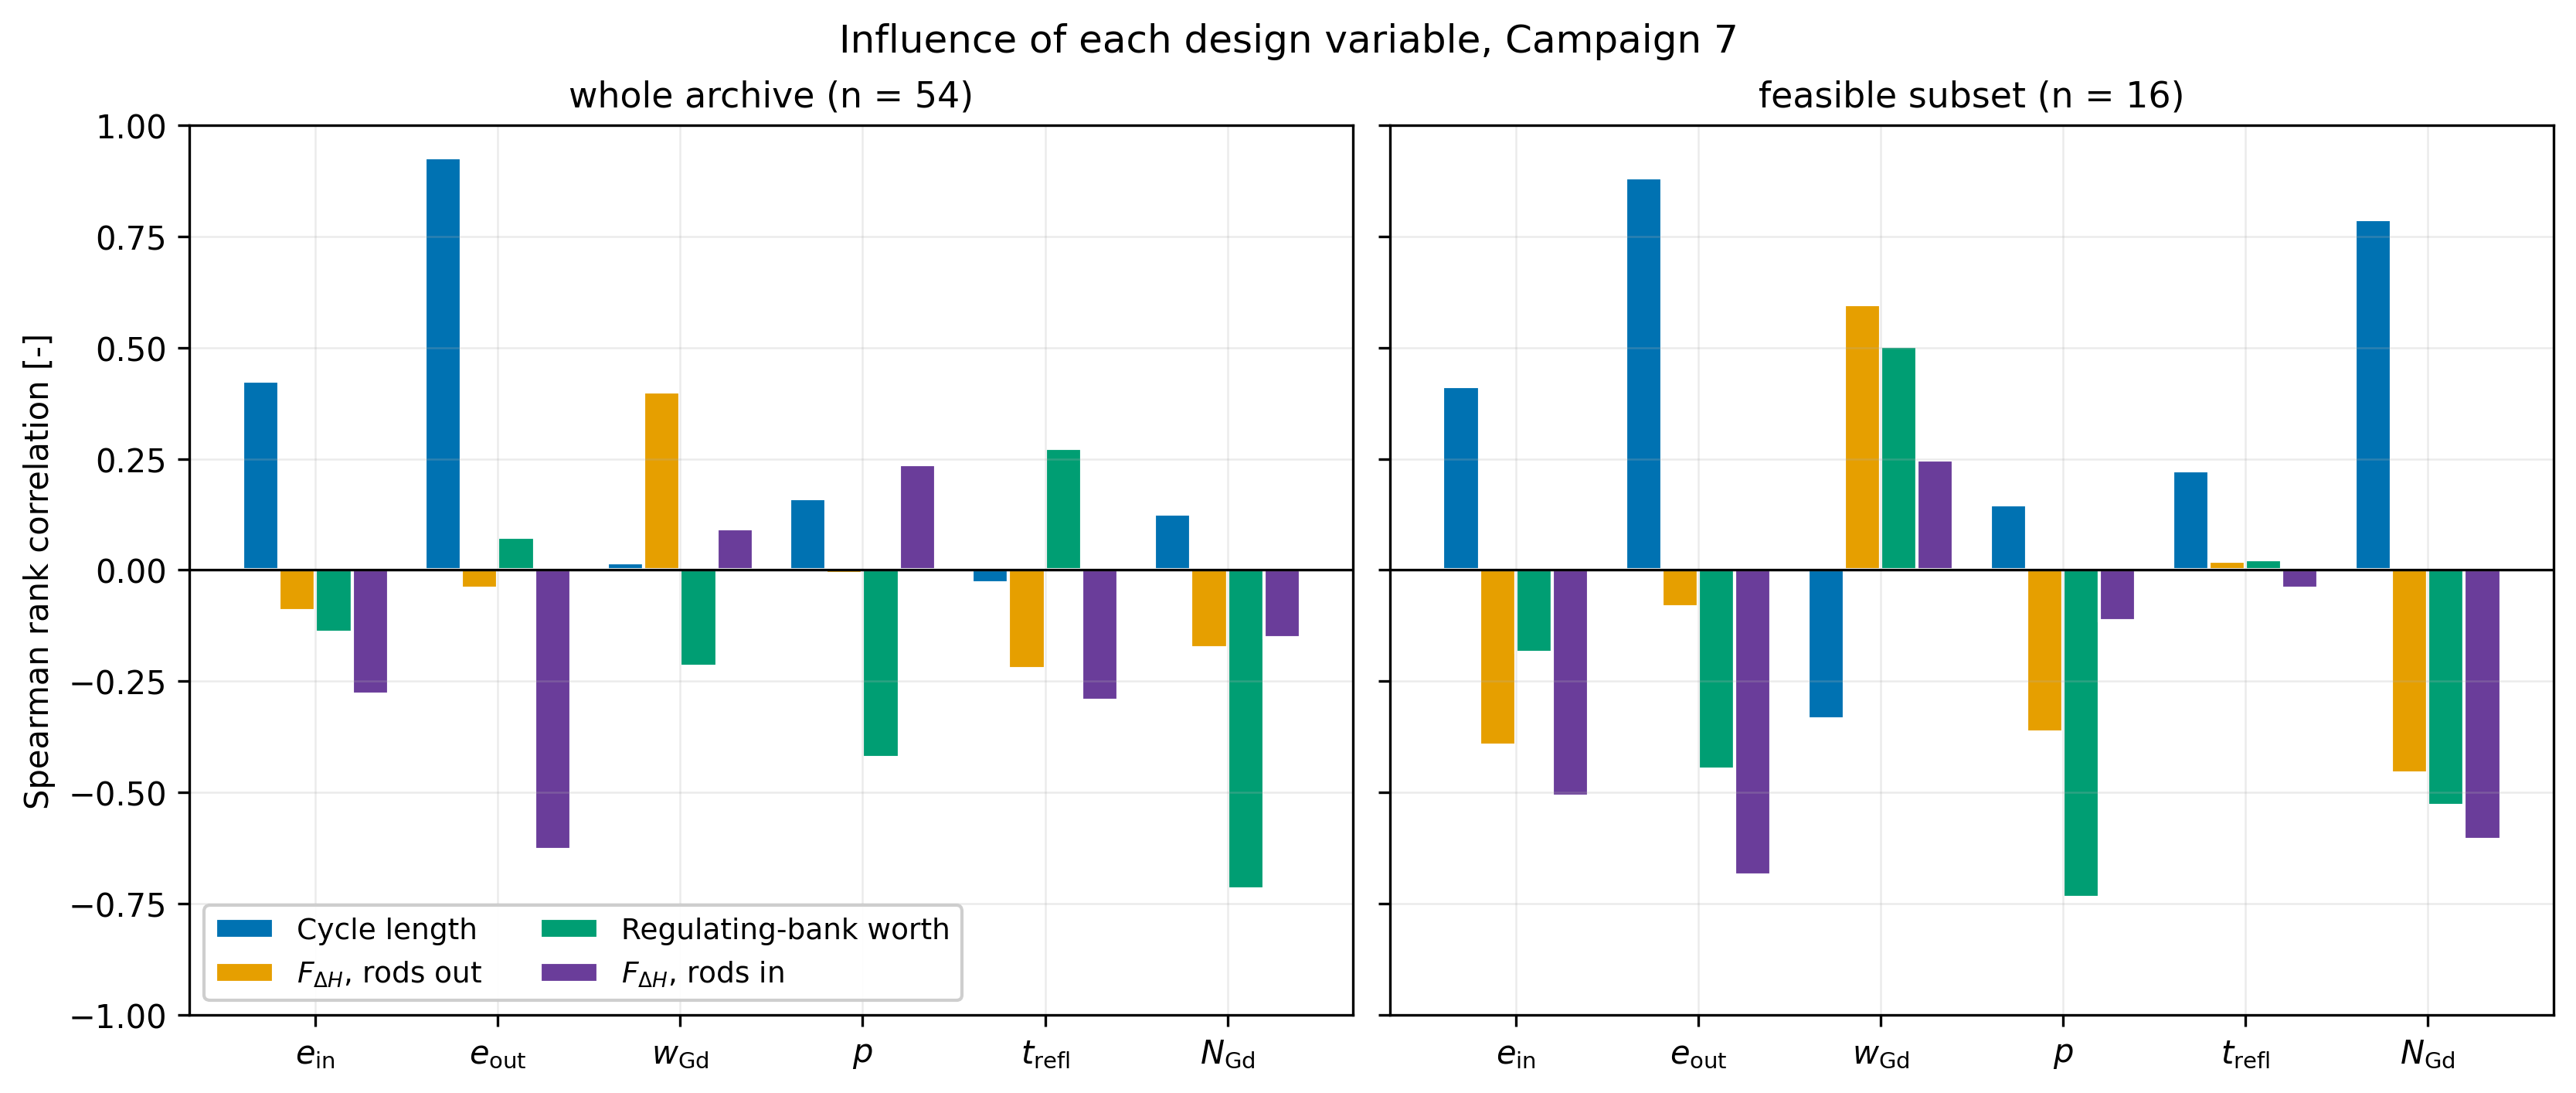
\includegraphics[width=\linewidth]{images/c7_vars_influence}
  \caption{Campaign 7: Spearman rank correlation of each design variable with the objectives, the regulating-bank worth and the rodded peaking.}
  \label{fig:c7-influence}
\end{figure}

The worth correlates at $-0.68$ with the gadolinium pin count, at
$-0.45$ with the pitch and at $+0.61$ with the unrodded eigenvalue.
Gadolinium depresses the eigenvalue and the bank worth together, so the
designs with the least worth are the heavily poisoned ones, which are
already far below the ceiling for a different reason. That is why the
two screens nest in this design space, and it is also why the
eight-design derivation of the ceiling looked safe when it was not.
The eight designs were all high-enrichment, forty-pin designs from one
corner of the Campaign 6 front, and their worths were alike because
their poison inventories were alike.

The measurement also settles a question left open since Campaign 4.
The ceiling of 1.35 used in Campaigns 1 to 6 was described as a
screening value not traceable to a primary source. Deriving the
ceiling from the worth of all seven banks, that is all 32 control rod
assemblies, with the same \SI{1000}{pcm} margin gives 1.368. The value
used through six campaigns sits two per cent below the measured
all-bank controllability bound of this core. It is a measured quantity
in retrospect, and the methodology chapter now states it as such,
with the caveat that an all-bank insertion with a \SI{1000}{pcm}
operating margin is not a licensing shutdown margin, which also
requires the highest-worth assembly stuck out and the cold, xenon-free
state.

\subsection{Peaking with the regulating banks inserted}
\label{sec:res-c7-rodded}

The peaking objective is evaluated with all rods out. The same core
solve that measures $k_\mathrm{RE}$ also yields the radial peaking
with the sixteen banks inserted, and Figure~\ref{fig:c7-rodded} plots
the two against each other. Every design lies above the screening bound
of 2.0 in the rodded configuration.

\begin{figure}[htbp]
  \centering
  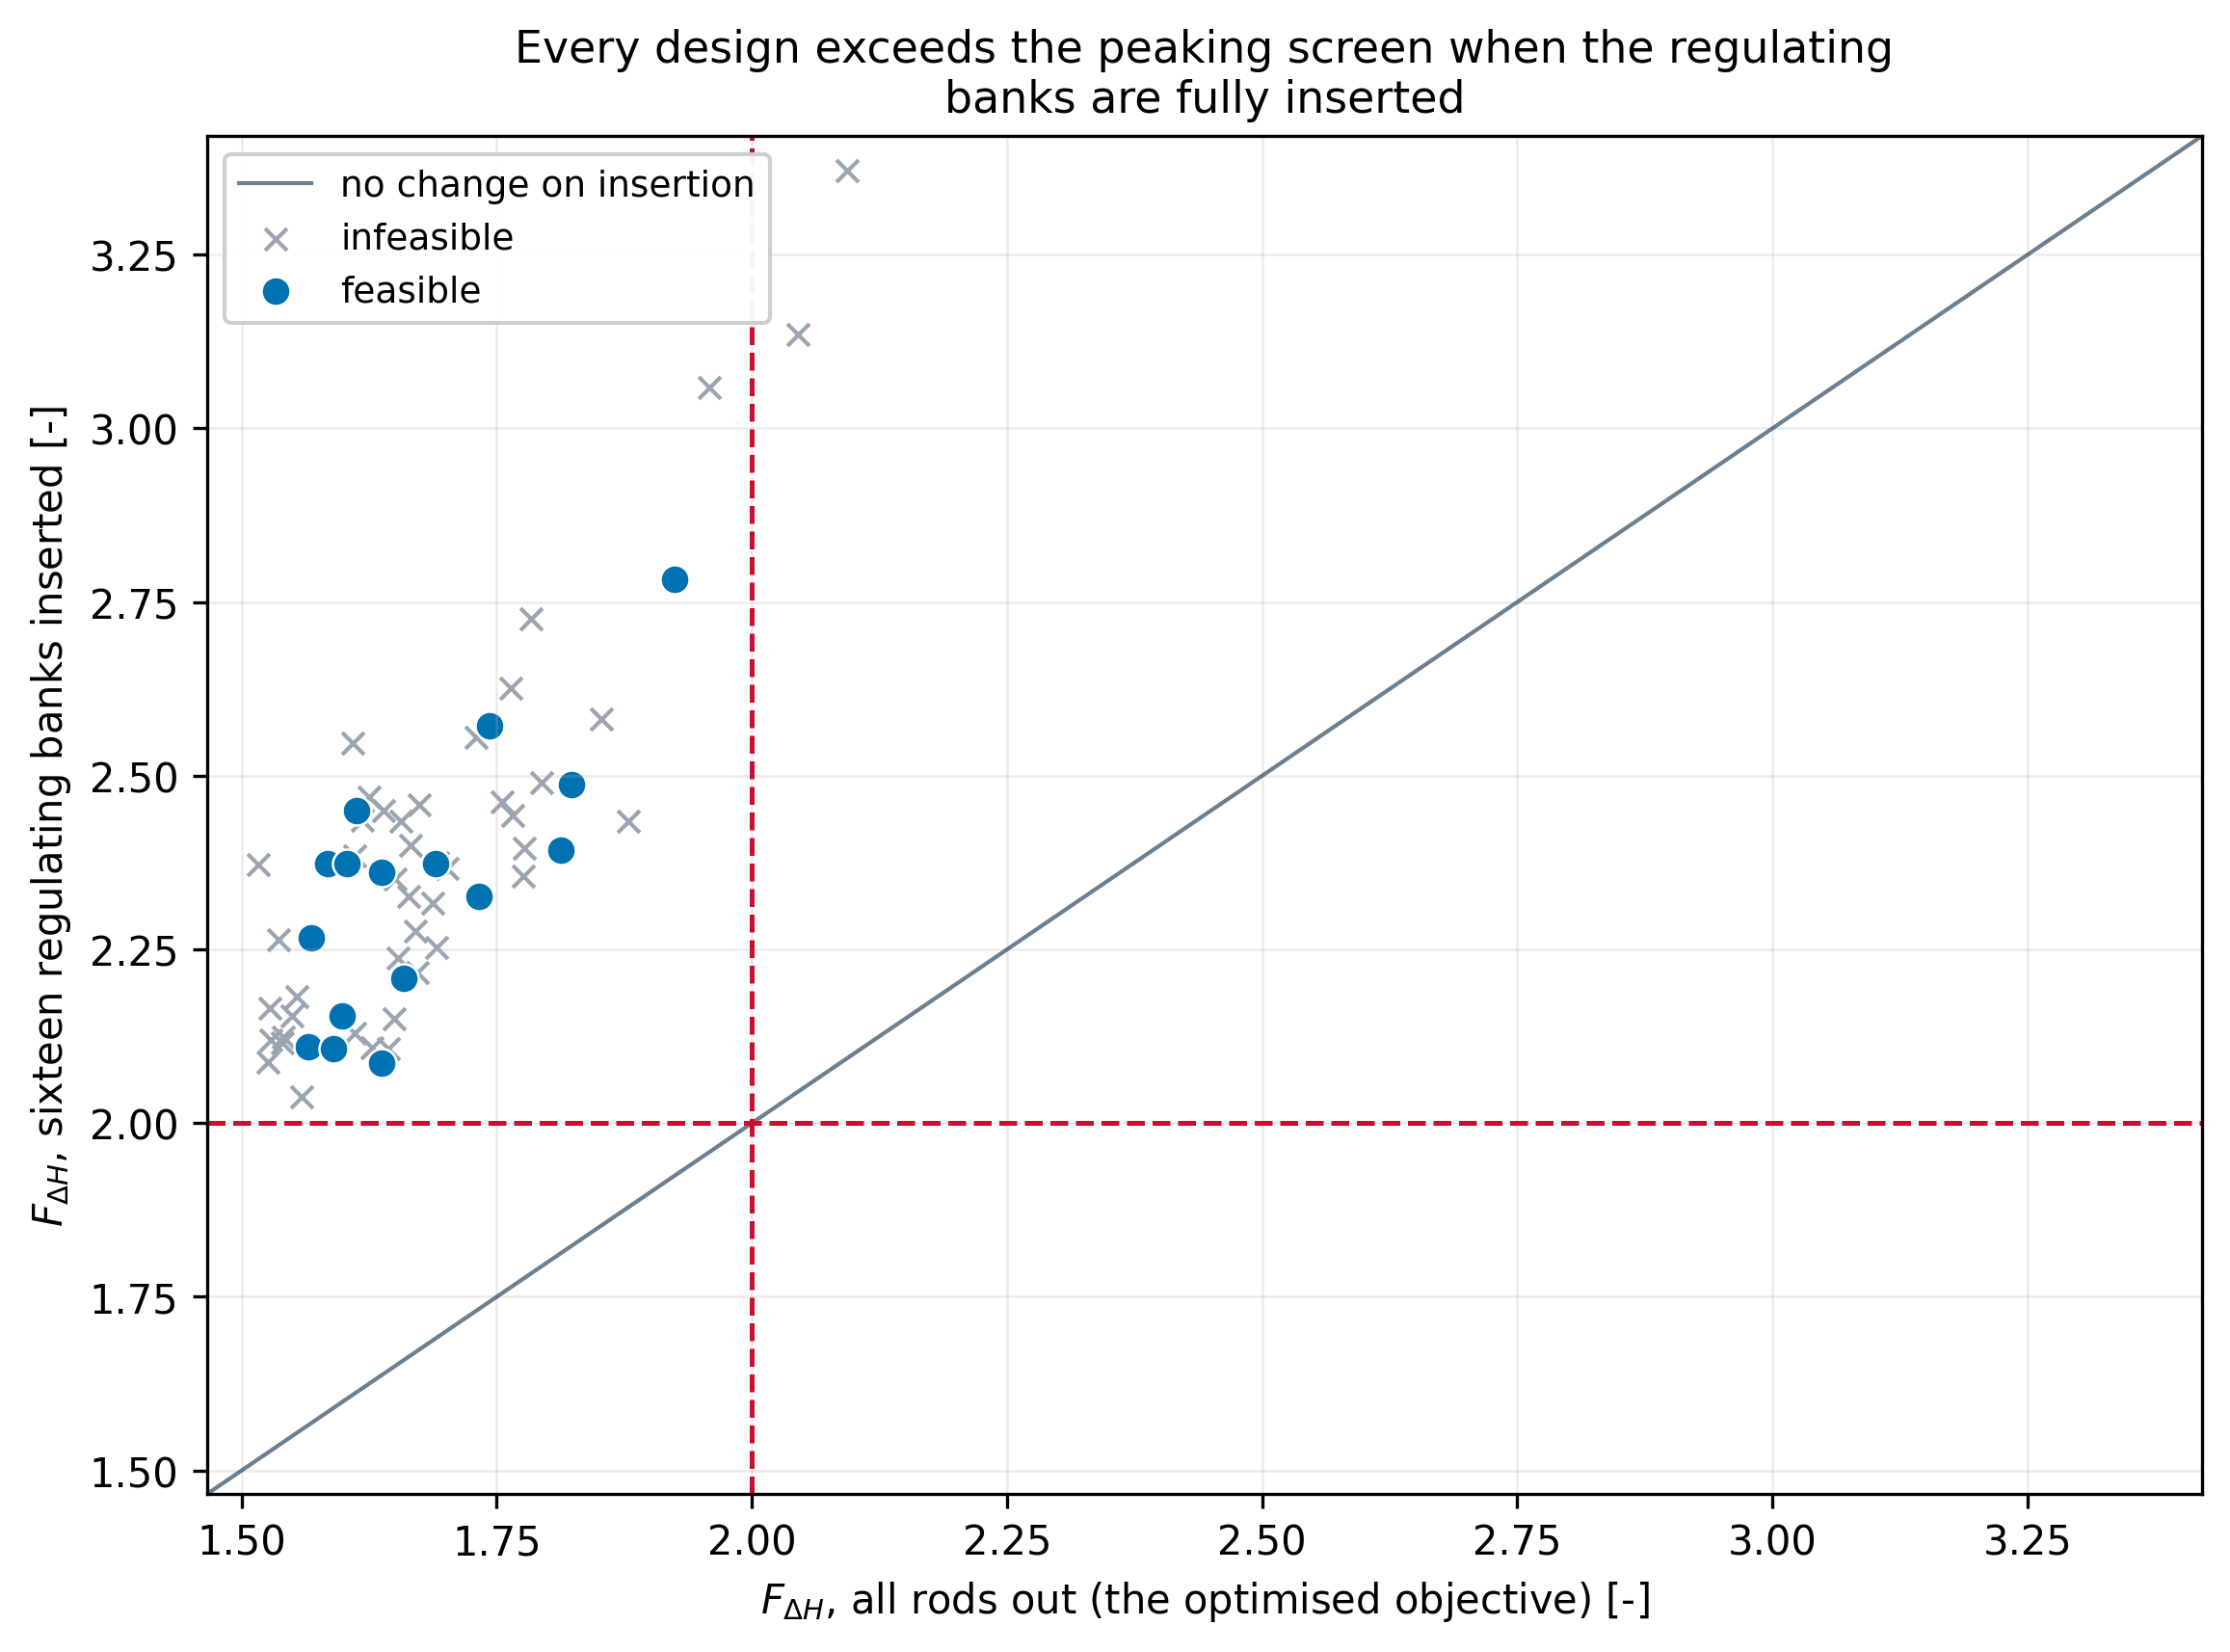
\includegraphics[width=0.85\linewidth]{images/c7_rodded_peaking}
  \caption{Campaign 7 radial peaking with all rods out against the same quantity with the sixteen regulating banks inserted.}
  \label{fig:c7-rodded}
\end{figure}

With the banks inserted $F_{\Delta H}$ runs from 2.038 to 3.371 with a
mean of 2.375, against 1.516 to 2.093 unrodded. The insertion penalty
ranges from 0.449 to 1.278 and is design dependent, correlating at
$-0.81$ with the outer-zone enrichment over the archive. Every one of
the 60 designs exceeds the screening bound of 2.0 in the rodded
configuration, and the three front designs sit between 2.11 and 2.16.

Two framings are required and neither should be overstated. Sixteen
banks fully inserted is the extreme of the regulating band used here as
a controllability test, not an operating configuration, so the rodded
value is an upper bound on operating peaking rather than an operating
value. Even so, the objective being minimised moves by half a unit or
more when the rods go in, and it moves by a design-dependent amount.
A design selected for low unrodded peaking is not thereby a design
with low rodded peaking. This is recorded as a limitation of the
objective set and as the motivation for the two-level reading of
Campaign 8.

%% AUTHOR: physical interpretation of the negative correlation between
%% the insertion penalty and the outer-zone enrichment.

\subsection{Depletion histories and the statistical error on the cycle length}
\label{sec:res-c7-uncertainty}

The assembly depletion solves are the only transport runs whose output
reaches the campaign log, and the log therefore holds the complete
$k_\infty(B)$ history of every design. Figure~\ref{fig:c7-histories}
reconstructs all 60 histories with the end-of-cycle crossing of the
leakage-corrected target marked in red, feasible designs on the left.
The gadolinium burnout maximum is visible between \num{7.5} and
\SI{17.5}{MWd/kgHM}, and no design approaches the \SI{75}{MWd/kgHM}
screen.

\begin{figure}[htbp]
  \centering
  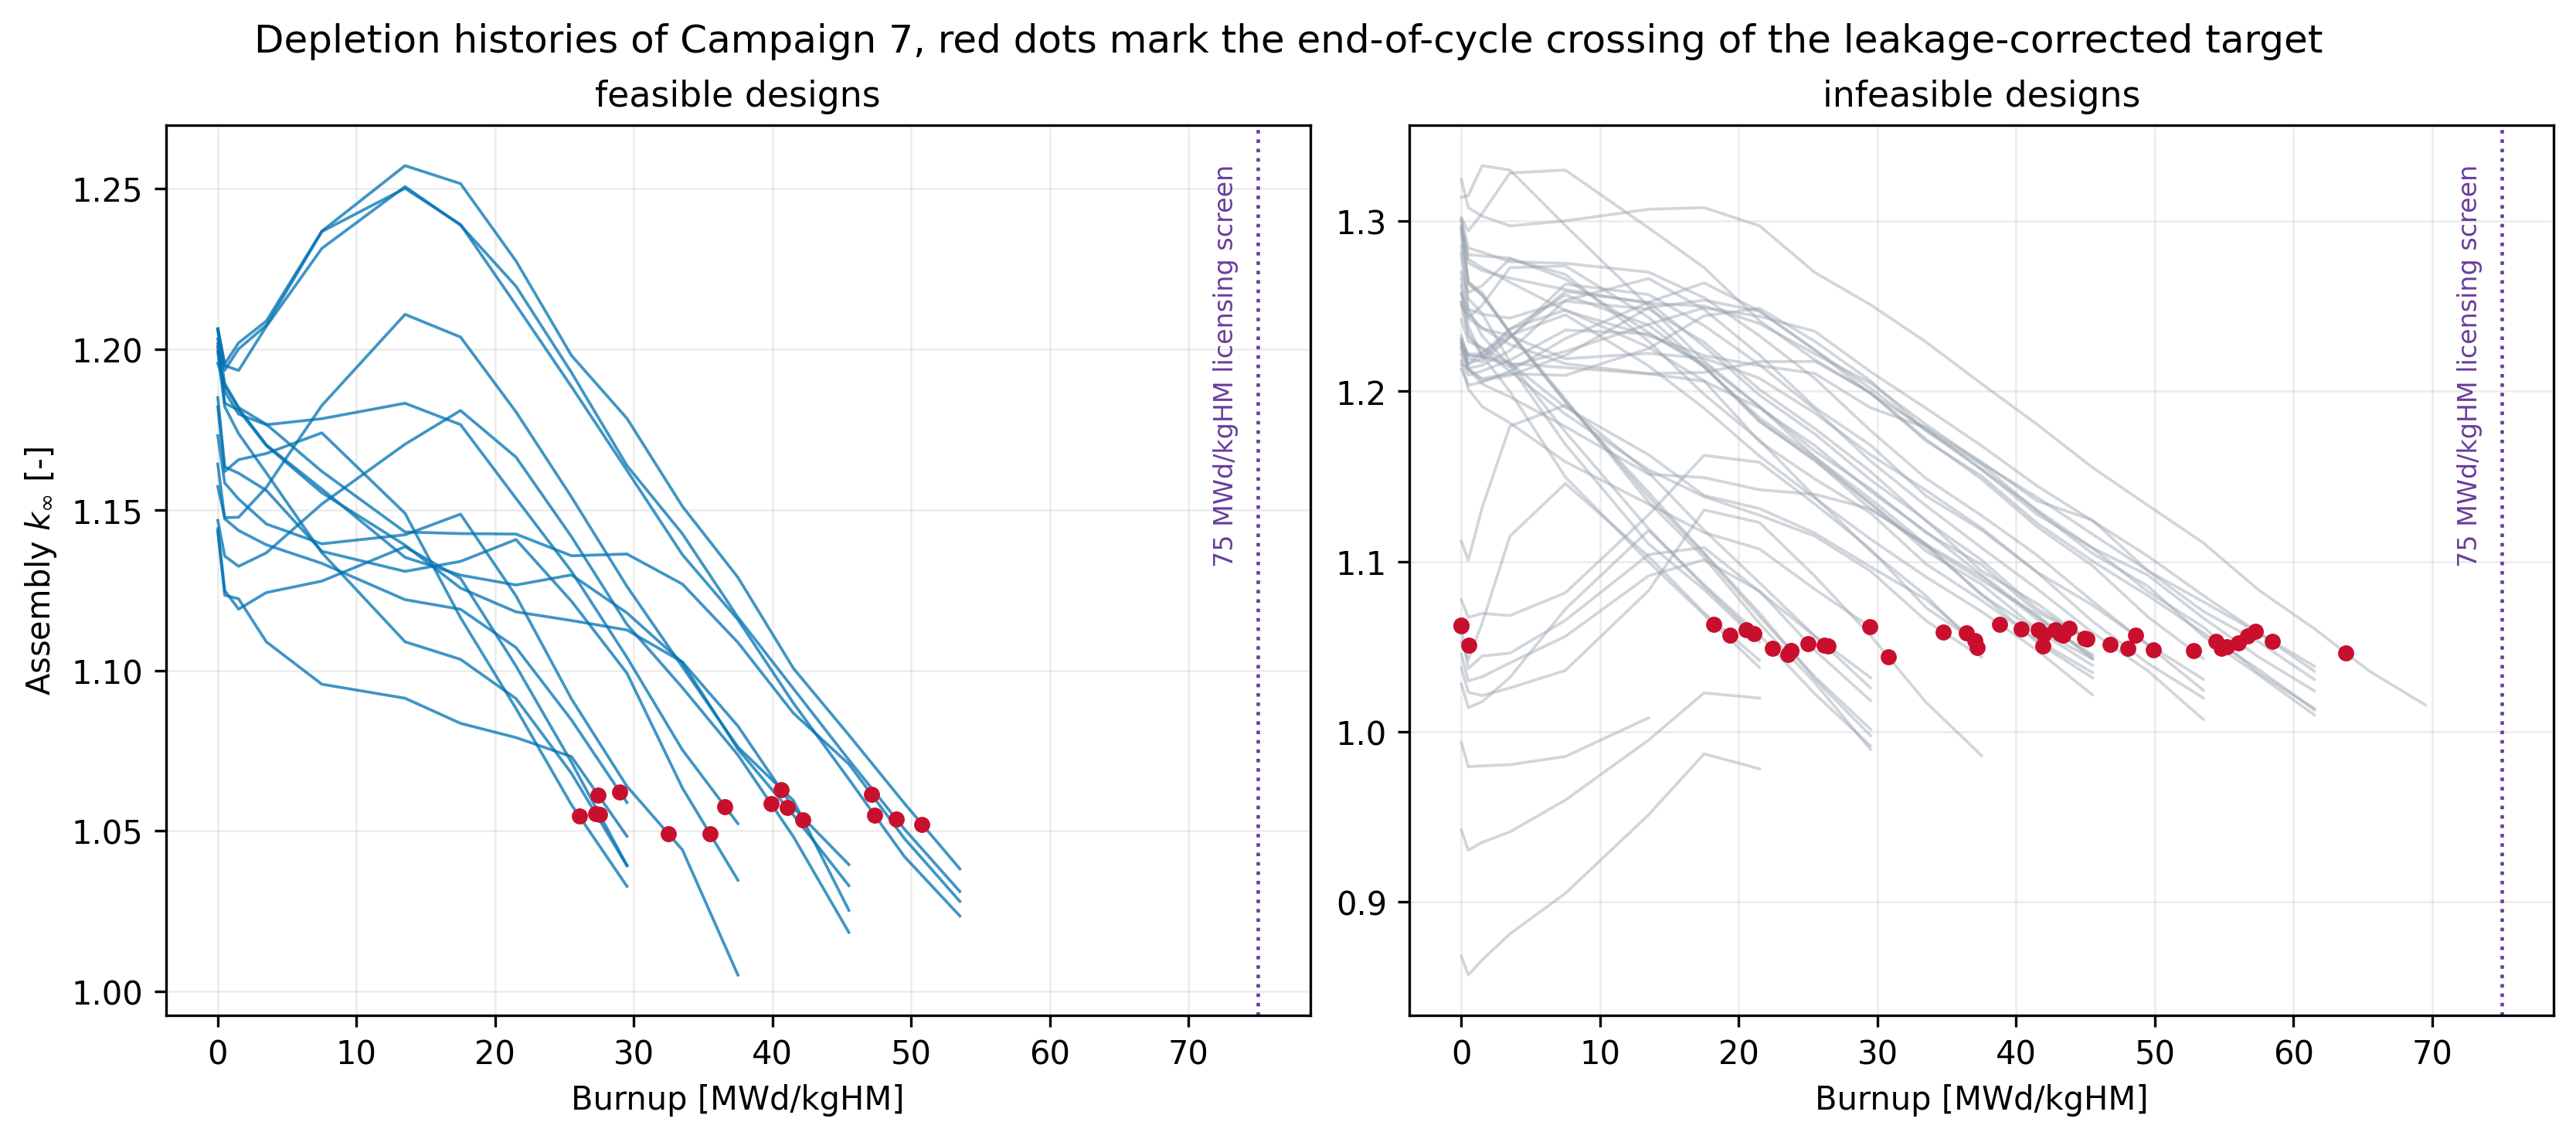
\includegraphics[width=\linewidth]{images/c7_kinf_histories}
  \caption{Assembly infinite multiplication factor against burnup for every Campaign 7 design.}
  \label{fig:c7-histories}
\end{figure}

The reconstruction was validated against the archive. Taking the last
descending crossing of the target reproduces the stored end-of-cycle
burnup of all 57 crossing designs to within \SI{0.0011}{MWd/kgHM}. The
last crossing is the correct rule because the gadolinium burnout makes
the early history non-monotonic. The three designs without a crossing
are the two subcritical cores at zero cycle length and one design
ending at 55 EFPD.

Three facts follow from the figure. The gadolinium hump raises
$k_\infty$ by up to \num{0.119} before the decline, measured in
Section~\ref{sec:res-c7-hump}. The highest end-of-cycle
burnup in the campaign is \SI{63.8}{MWd/kgHM}, so the
\SI{75}{MWd/kgHM} discharge screen of Section~\ref{sec:meth-atf} is
inactive and no design is censored, unlike Campaign 6. And the local
slope at end of cycle is steep, which governs the statistical error on
the cycle length.

The Monte Carlo error on the cycle length is obtained by propagating
the uncertainties of the two transport states that bracket the
crossing.

\begin{equation}
\sigma_B^2 = \left(\frac{\Delta B\,(k_\mathrm{t} - k_{j+1})}{(k_j - k_{j+1})^2}\right)^2 \sigma_{k_j}^2
+ \left(\frac{\Delta B\,(k_j - k_\mathrm{t})}{(k_j - k_{j+1})^2}\right)^2 \sigma_{k_{j+1}}^2
\label{eq:sigma-beoc}
\end{equation}

\noindent where the symbols have the following meaning.

\begin{itemize}
  \item $\sigma_B$ is the statistical uncertainty of the end-of-cycle
        burnup, in MWd/kgHM.

  \item $\Delta B$ is the burnup step between the two bracketing
        states, in MWd/kgHM.

  \item $k_j$ and $k_{j+1}$ are the infinite multiplication factors at
        the states before and after the crossing, dimensionless.

  \item $k_\mathrm{t}$ is the leakage-corrected target, dimensionless,
        treated as exact.

  \item $\sigma_{k_j}$ and $\sigma_{k_{j+1}}$ are the reported Monte
        Carlo standard deviations of the two states, dimensionless.
\end{itemize}

The cycle length follows from the specific power.

\begin{equation}
\sigma_\mathrm{EFPD} = \frac{1000\,\sigma_B}{P_\mathrm{sp}}
\label{eq:sigma-efpd}
\end{equation}

\noindent where the symbols have the following meaning.

\begin{itemize}
  \item $\sigma_\mathrm{EFPD}$ is the statistical uncertainty of the
        cycle length, in effective full power days.

  \item $P_\mathrm{sp}$ is the specific power of the core,
        \SI{9.98}{W/gHM}.
\end{itemize}

Figure~\ref{fig:c7-uncertainty} plots the propagated error against the
cycle length and against the reactivity slope at end of cycle. The error
is set by the slope at end of cycle, and the length of the cycle does
not govern it.

\begin{figure}[htbp]
  \centering
  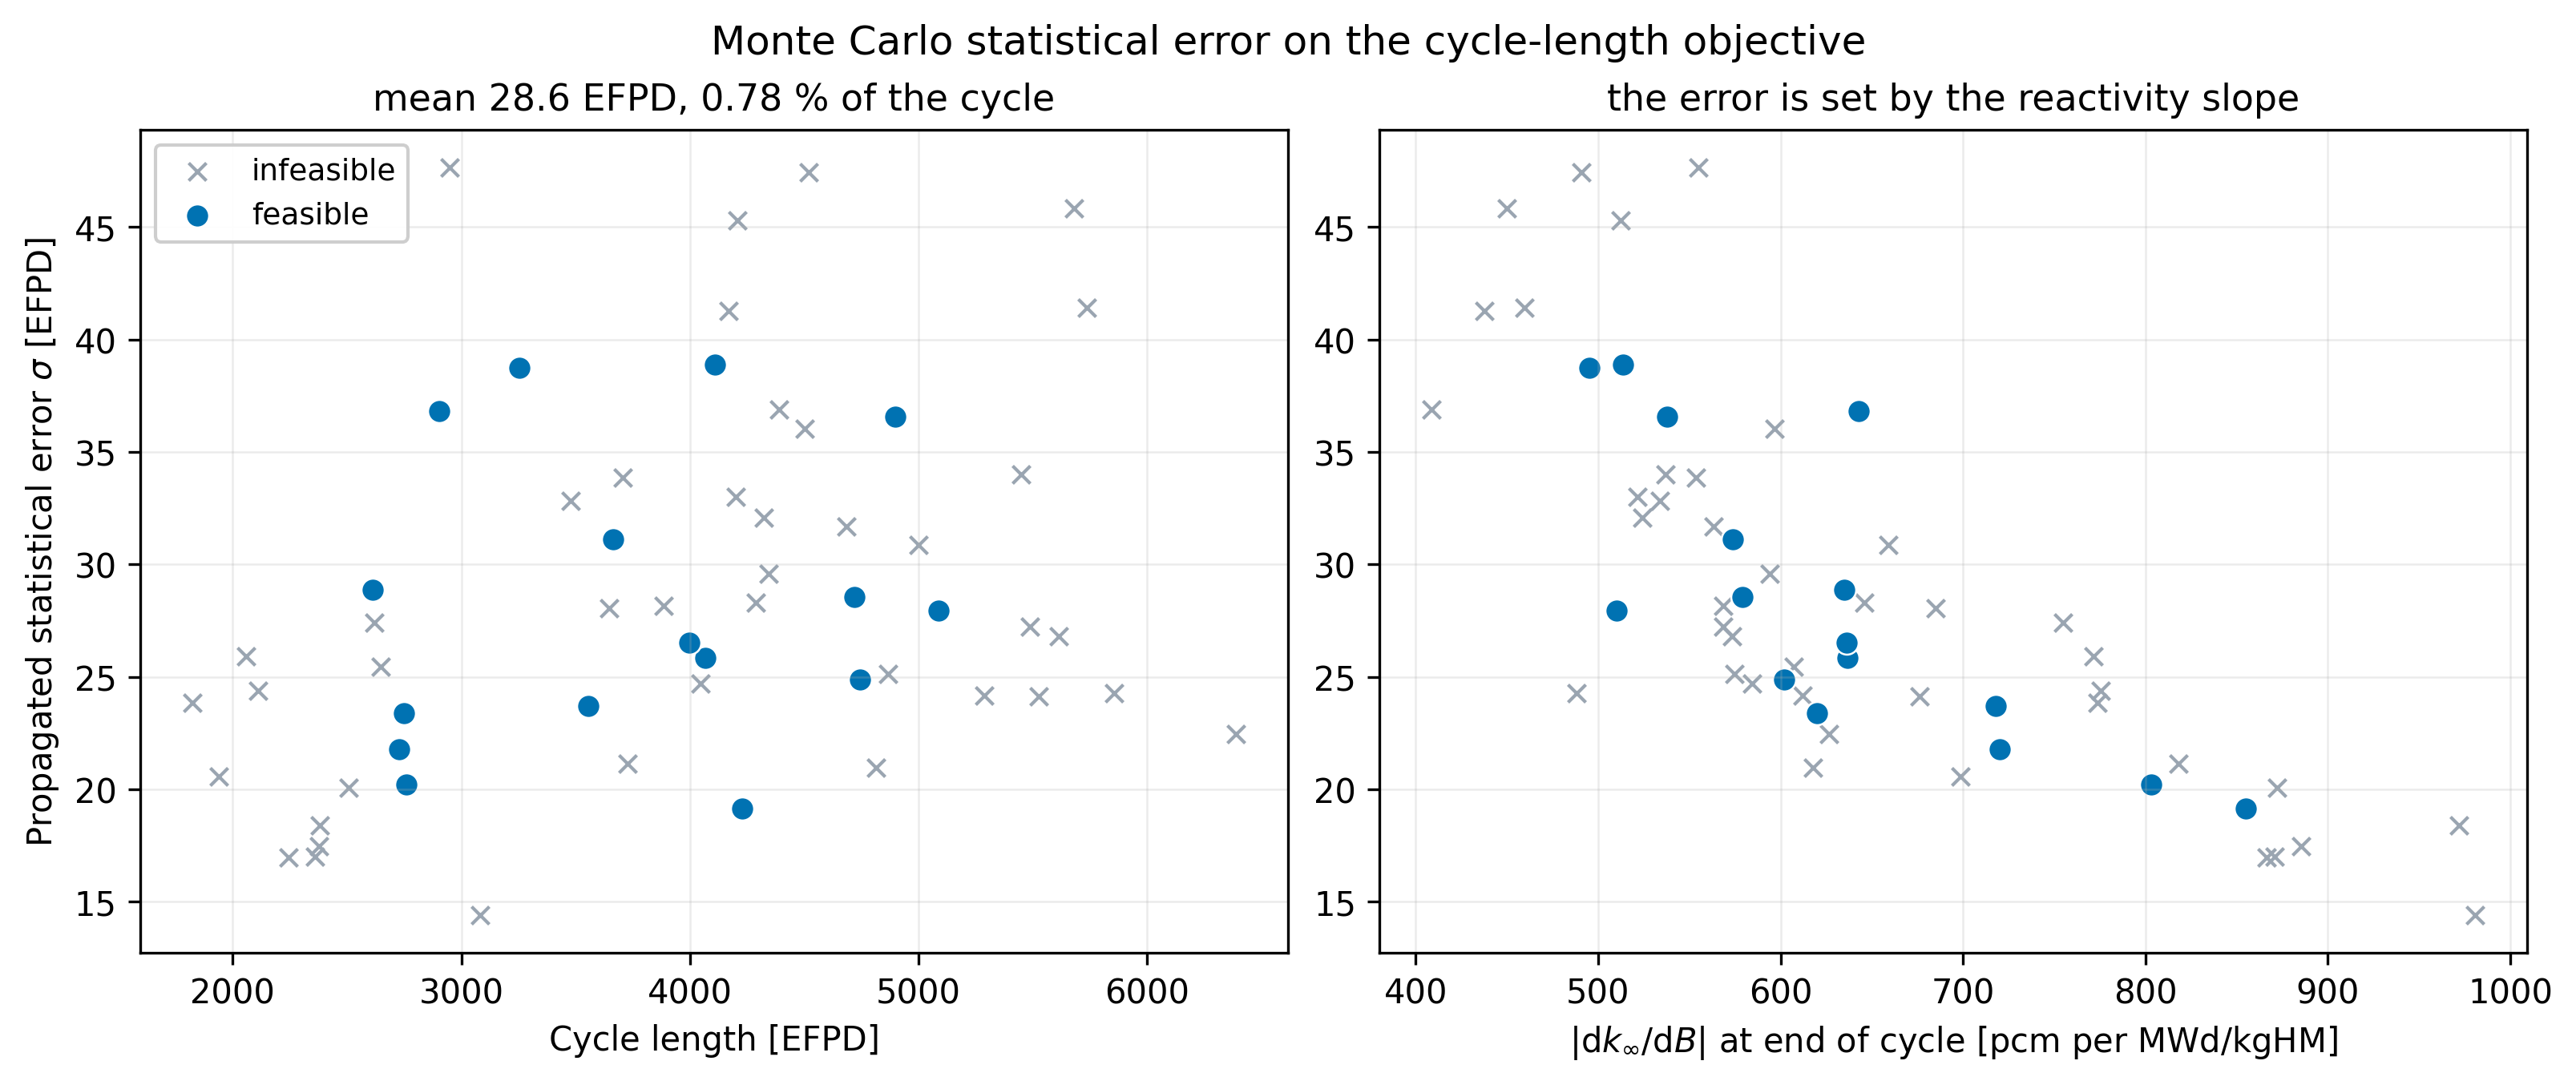
\includegraphics[width=\linewidth]{images/c7_cycle_uncertainty}
  \caption{Propagated Monte Carlo error on the Campaign 7 cycle length.}
  \label{fig:c7-uncertainty}
\end{figure}

Table~\ref{tab:c7-uncertainty} summarises the result and
Figure~\ref{fig:c7-uncertainty} shows it. The slope at end of cycle
lies between 409 and \SI{981}{pcm} per MWd/kgHM with a median of 607.
The resulting error has a mean of 28.6 EFPD, \SI{0.78}{\%} of the
cycle, and a worst case of 47.7 EFPD, \SI{1.62}{\%}. On the six front
designs it is 25 to 37 EFPD. The smallest gap between adjacent front
designs is 154 EFPD, about five standard deviations, so the ordering of
the front in cycle length is statistically resolved.

\begin{table}[htbp]
  \centering
  \caption{Statistical error on the cycle length over the 57 designs
  with a resolved end-of-cycle crossing.}
  \label{tab:c7-uncertainty}
  \begin{tabular}{lccc}
    \toprule
    Quantity & Minimum & Median & Maximum \\
    \midrule
    Slope at end of cycle [pcm per MWd/kgHM] & 409 & 607 & 981 \\
    Bracketing sigma on $k_\infty$ [pcm]     & 178 & 218 & 274 \\
    $\sigma_\mathrm{EFPD}$ [d]               & 14.4 & 27.2 & 47.7 \\
    $\sigma_\mathrm{EFPD}$ as a fraction of the cycle [\%] & 0.35 & 0.74 & 1.62 \\
    \bottomrule
  \end{tabular}
\end{table}

The peaking axis is the opposite case. The front designs are separated
by 0.003 to 0.036 in $F_{\Delta H}$, the entropy study of
Section~\ref{sec:res-c6} bounded the systematic shift at $\pm 0.02$,
and no statistical error on the core peaking tally has been measured.
The ordering of the front in peaking is therefore not resolved, and
designs 59, 57 and 55 at 1.525, 1.528 and 1.529 must be treated as
indistinguishable until the tally errors are read from the statepoints.

\openpoint{Measure $\sigma(F_{\Delta H})$ from the per-bin relative
errors of the core mesh tally on the six front designs, or by seed
replicates, before any ordering claim on the peaking axis is made.}

\subsection{The gadolinium hump in the Campaign 7 archive}
\label{sec:res-c7-hump}

The histories of Section~\ref{sec:res-c7-uncertainty} carry a second
measurement that the crossing analysis does not use. Between beginning
of life and the end-of-cycle decline, the assembly eigenvalue of a
gadolinia-bearing design first rises, because the poison burns out
faster than the fuel. The maximum of that rise, and not the beginning
of life, is the most reactive state the core ever occupies. Any
reactivity screen written at beginning of life therefore screens the
wrong state whenever a hump is present.

The hump is defined on the reactivity scale.

\begin{equation}
  \Delta\rho_\mathrm{hump} = \rho\!\left(k_\mathrm{peak}\right) -
  \rho\!\left(k_\mathrm{BOL}\right),
  \qquad
  \rho(k) = 10^{5}\,\frac{k-1}{k}
  \label{eq:c7-hump}
\end{equation}

where the symbols have the following meaning.

\begin{itemize}
  \item $\Delta\rho_\mathrm{hump}$ is the reactivity gained between
        beginning of life and the operating maximum, in pcm.
  \item $k_\mathrm{BOL}$ is the assembly infinite multiplication factor
        at zero burnup, xenon-free, at \SI{1000}{ppm} soluble boron,
        dimensionless.
  \item $k_\mathrm{peak}$ is the maximum of the assembly infinite
        multiplication factor over the operating points, dimensionless.
  \item $\rho$ is the reactivity, in pcm.
\end{itemize}

Figure~\ref{fig:c7-khist-gd} shows the same histories as
Figure~\ref{fig:c7-histories}, coloured by gadolinia weight fraction
instead of by feasibility, and Table~\ref{tab:c7-hump} lists the
fifteen designs with the largest humps.

\begin{figure}[htbp]
  \centering
  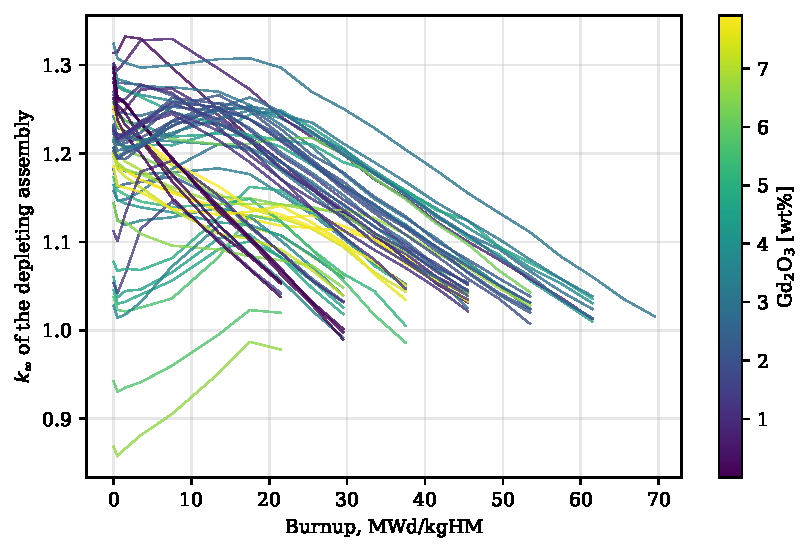
\includegraphics[width=0.95\linewidth]{images/k_histories}
  \caption[Campaign 7 histories coloured by gadolinia loading]{Assembly
  infinite multiplication factor against burnup for the Campaign 7
  archive, coloured by the gadolinia weight fraction of the design.}
  \label{fig:c7-khist-gd}
\end{figure}

\begin{table}[htbp]
  \centering
  \footnotesize
  \setlength{\tabcolsep}{3.5pt}
  \caption[Reactivity hump of the Campaign 7 designs]{Gadolinium hump and burnup reactivity swing of the Campaign 7 designs, recovered from the run log.}
  \label{tab:c7-hump}
  \begin{tabular}{@{}r r r r r r r r@{}}
    \toprule
    ID & $e_\mathrm{in}/e_\mathrm{out}$ & Gd & $k_\mathrm{BOL}$ & $k_\mathrm{peak}$ & $B_\mathrm{peak}$ & hump & $\Delta\rho_\mathrm{peak\to EOC}$ \\
    {[--]} & [wt\%] & [wt\%] & [--] & [--] & [MWd/kgHM] & [pcm] & [pcm] \\
    \midrule
    34 & 4.48/3.14 & 6.59 & 0.8681 & 0.9870 & 17.5 & +13874 & -7158 \\
    4 & 5.38/3.89 & 5.72 & 0.9423 & 1.0228 & 17.5 & +8352 & -3663 \\
    27 & 5.32/5.52 & 5.60 & 1.0376 & 1.1302 & 17.5 & +7901 & 7312 \\
    38 & 4.39/4.20 & 3.61 & 1.0279 & 1.1182 & 13.5 & +7864 & 5918 \\
    26 & 4.88/3.78 & 1.54 & 1.0530 & 1.1457 & 7.5 & +7690 & 7344 \\
    29 & 3.11/7.99 & 4.83 & 1.0774 & 1.1623 & 17.5 & +6781 & 8892 \\
    39 & 9.91/3.21 & 1.12 & 1.1118 & 1.1917 & 7.5 & +6035 & 11297 \\
    15 & 9.08/3.40 & 4.73 & 1.0454 & 1.1009 & 17.5 & +4821 & 4231 \\
    22 & 7.35/3.95 & 4.54 & 1.0604 & 1.1082 & 17.5 & +4069 & 4914 \\
    16 & 3.31/8.68 & 2.99 & 1.1573 & 1.2109 & 13.5 & +3826 & 12335 \\
    49 & 8.92/7.99 & 2.23 & 1.2064 & 1.2572 & 13.5 & +3351 & 15508 \\
    50 & 8.99/8.73 & 2.71 & 1.2130 & 1.2635 & 17.5 & +3300 & 16085 \\
    48 & 8.71/7.80 & 1.93 & 1.2033 & 1.2502 & 13.5 & +3118 & 14811 \\
    53 & 8.77/7.86 & 2.05 & 1.2065 & 1.2507 & 13.5 & +2934 & 14939 \\
    51 & 8.98/9.16 & 2.89 & 1.2158 & 1.2534 & 17.5 & +2469 & 15260 \\
    \bottomrule
  \end{tabular}
\end{table}

Four readings follow from the table.

\begin{enumerate}
  \item The hump is large. The largest, design 34, gains
        \SI{13874}{pcm} between beginning of life and its maximum, and
        the fifteenth of the list still gains \SI{2469}{pcm}. On the
        eigenvalue scale design 34 moves from \num{0.8681} to
        \num{0.9870}, a rise of \num{0.119}.

  \item The maximum does not sit at a single burnup. The recovered
        maxima fall at \num{7.5}, \num{13.5} and
        \SI{17.5}{MWd/kgHM}, and the earliest of them belong to the
        two designs with the lowest gadolinia loading of the list,
        designs 26 and 39 at \num{1.54} and \SI{1.12}{wt\%}.

  \item The hump is not ordered by gadolinia weight fraction alone.
        Design 26 gains \SI{7690}{pcm} at \SI{1.54}{wt\%} while design
        51 gains \SI{2469}{pcm} at \SI{2.89}{wt\%}, so the poisoned-pin
        count and the enrichment split enter as well.

  \item The two designs whose swing from the maximum to end of cycle is
        negative, designs 34 and 4, are the two whose beginning-of-life
        eigenvalue is below unity. Their cycle ends before the poison
        has finished burning out.
\end{enumerate}

This measurement is the reason the Campaign 8 analysis reports the
hump for every candidate in Section~\ref{sec:res-c8-swing}, and the
reason the reactivity screens of this work are read at the operating
maximum rather than at beginning of life alone.

%% AUTHOR: the physics of the hump, namely why the poison burnout can
%% outrun the fuel depletion by more than 10000 pcm in this lattice,
%% and whether the beginning-of-life screen of
%% Section~\ref{sec:meth-ctrl} should have been written at the maximum
%% from the start.

\subsection{Cost and instrumentation}
\label{sec:res-c7-cost}

The campaign cost \SI{56965}{s} of wall time, \SI{949}{s} per
evaluation, against \SI{840}{s} in Campaign 6. The difference is the
control solve. Two instrumentation defects were found while reading
the archive, and both are recorded because they affect numbers reported
elsewhere in this chapter.

\begin{enumerate}
  \item The per-evaluation cost stored in the archive excludes the
        control solve, because that solve is invoked after the three
        timers close. Over the campaign the control solves are
        \SI{11}{\%} of the true cost and \SI{12.6}{\%} of the reported
        cost. The wall-clock figure of the block log is correct and is
        the one quoted above. The evaluator is corrected from Campaign
        8 (Section~\ref{sec:meth-cost}).

  \item The per-case parser of the run log never matched a single case
        line of any campaign, because the censoring marker inserted
        after the cycle length was not anticipated by its regular
        expression. The failure was silent, and every per-case table
        the parser produced before the correction was empty. No number
        in this chapter depends on that table, since all per-design
        quantities are read from the archive.
\end{enumerate}

\subsection{Limitations and the settings carried forward}
\label{sec:res-c7-limits}

Four limitations bound the claims of this section.

\begin{enumerate}
  \item Four designs, 10, 32, 41 and 43, reached the active batches
        with the Shannon entropy of the fission source not yet
        converged, the worst at 105 of 60 inactive batches. None is on
        either front. Their eigenvalues and peaking values carry an
        unquantified bias, are retained in the archive statistics of
        this section with that caveat, and are excluded from any
        candidate list.

  \item Twenty-five of the 60 designs have a pitch below
        \SI{1.2242}{cm}, twice the guide-tube outer radius. Below that
        value the lattice clips the guide-tube wall at the cell
        boundary silently, replacing up to \SI{27}{\%} of the wall
        cross-section by moderator at the box minimum of
        \SI{1.150}{cm}. Designs 57 and 59, the two lowest-peaking
        designs of the control-screen front, are both in the affected
        band. The same defect reaches back to every earlier campaign
        design at pitches below \SI{1.2242}{cm}, including the
        Campaign 4 infill designs pinned at the box minimum and the
        Campaign 6 discharge-screen champion at \SI{1.150}{cm}. Fixing
        the pitch at \SI{1.26}{cm} in Campaign 8 removes the defect
        prospectively, and a caveat is added to the affected results.

  \item The statistical error on the peaking objective is not
        measured, as stated above.

  \item Every cycle length in this campaign, as in all earlier ones, is
        a two-dimensional value. The axial leakage study of
        Section~\ref{sec:meth-lax}, completed after this campaign,
        measured the axial correction at \num{1.0282} to \num{1.0298}
        on six Campaign 6 designs, about \SI{3000}{pcm} of reactivity,
        which at the end-of-cycle slopes measured here corresponds to
        roughly 450 to 500 EFPD. Campaign 7 cycle lengths are therefore
        overstated by that amount relative to a finite-height core,
        uniformly across the archive, and the ordering of the front is
        unaffected. Campaign 8 carries the correction inside the
        end-of-cycle target from the start.
\end{enumerate}

What carries forward is the constraint architecture. The measured
control screen replaces the derived ceiling as the reactivity
constraint that does the work, a second reading with only the first two
banks inserted is added and recorded, the axial factor enters the
target, the acquisition settings of Campaign 6 are restored explicitly,
and the pitch is fixed at the value that both closes the geometric
defect and matches the reference fuel design. Section~\ref{sec:res-c8}
states the campaign built on those decisions.


\section{Campaign 8: the candidate campaign}
\label{sec:res-c8}

Campaign 8 is the last campaign of the original formulation, and its
front is the set of candidate cores under that formulation. It fixes what the earlier campaigns established and
measures what they could not. It ran 60 evaluations on wks720 in
\SI{21.02}{h}, every one of them completing without error, and every
cycle length it reports refers for the first time in this work to a
finite-height core, through the axially corrected target of
Equation~\eqref{eq:ktarget-3d}.

\subsection{Specification}
\label{sec:res-c8-intent}

Section~\ref{sec:meth-c8-space} states the design space and
Table~\ref{tab:c8-spec} the specification as launched. Three settings
were pre-registered as the ones under test. The measured control screen
of Section~\ref{sec:meth-ctrl} is the working reactivity constraint,
with the three-dimensional derived ceiling of 1.166 behind it. A second
rodded reading with only the first two regulating banks inserted is
recorded on every design and is not a constraint. And the acquisition
settings that Campaign 7 omitted are restored explicitly.

\begin{table}[htbp]
  \centering
  \small
  \caption{Campaign 8 as launched on 1 September 2026.}
  \label{tab:c8-spec}
  \begin{tabularx}{\textwidth}{@{}>{\raggedright\arraybackslash}p{4.0cm}>{\raggedright\arraybackslash}X@{}}
    \toprule
    Item & Setting \\
    \midrule
    Design variables & $e$ 3.0 to \SI{13.913}{wt\%}, the upper bound set by the \SI{16}{wt\%} peripheral cap, $w_\mathrm{Gd}$ 0 to \SI{8}{wt\%}, $t_\mathrm{refl}$ 2.0 to \SI{5.66}{cm}, $n_\mathrm{Gd}$ 12 to 40 on the ladder \\
    Fixed & pitch \SI{1.26}{cm}, active height \SI{120}{cm}, clearance \SI{7.08}{cm}, soluble boron \SI{1000}{ppm}, ring multipliers \num{0.720}, \num{0.893}, \num{1.150} \\
    Objectives & maximise EFPD, minimise $F_{\Delta H}$ with all rods out \\
    Reactivity window & $1.02 \le k_\mathrm{eff}^\mathrm{core} \le 1.166$ on the core basis \\
    Control screen & $k_\mathrm{RE} \le 0.99$, RE1 to RE4 inserted, B$_4$C, constrained \\
    Second reading & $k_\mathrm{RE12}$, RE1 and RE2 inserted, recorded only \\
    End of cycle & $k_\mathrm{target}^\mathrm{3D}$ from 1.0839 to 1.0820 \\
    Acquisition & minimum separation 0.14, feasibility margin 1.5 standard deviations \\
    Budget & design of experiments 36, four infill blocks of six \\
    Fidelity & depletion $4000\times60$, every core solve $100000\times170$ with 60 inactive \\
    \bottomrule
  \end{tabularx}
\end{table}

\subsection{Blocks, diversity and convergence}
\label{sec:res-c8-blocks}

Table~\ref{tab:c8-blocks} records the five blocks and
Figure~\ref{fig:c8-diversity} their diversity. The hypervolume is taken
against the frozen reference of 1760 EFPD and 2.096, and the spread is
the within-block range of each variable as a fraction of the archive
range, listed in the order $e$, $w_\mathrm{Gd}$, $t_\mathrm{refl}$,
$n_\mathrm{Gd}$. Every infill block
returned feasible designs and every block moved at least three of the
four variables. Block 1 held the gadolinia concentration fixed at
\SI{8.0}{wt\%} across its six designs while moving the other three
variables, a residual of the collapse mode of Campaign 7 in one
variable only. Figure~\ref{fig:c8-trajectory} shows the two objectives
in evaluation order, with the blocks separated by vertical lines. The
infill blocks concentrate on the long-cycle end of the feasible region,
where the control screen binds.

\begin{table}[htbp]
  \centering
  \caption{Campaign 8 blocks.}
  \label{tab:c8-blocks}
  \begin{tabular}{lcccl}
    \toprule
    Block & Designs & Feasible & Hypervolume (gain) & Spread \\
    \midrule
    DOE      & 36 & 9 & 1966.0 & 1.00, 0.99, 0.97, 0.99 \\
    Infill 1 &  6 & 3 & 1966.0 (0.00\,\%) & 0.50, 0.00, 0.33, 0.86 \\
    Infill 2 &  6 & 3 & 2022.4 (+2.87\,\%) & 0.66, 0.83, 0.65, 1.00 \\
    Infill 3 &  6 & 1 & 2022.4 (0.00\,\%) & 0.69, 0.68, 0.26, 1.00 \\
    Infill 4 &  6 & 3 & 2026.1 (+0.18\,\%) & 0.41, 0.62, 1.00, 0.53 \\
    \bottomrule
  \end{tabular}
\end{table}

\begin{figure}[htbp]
  \centering
  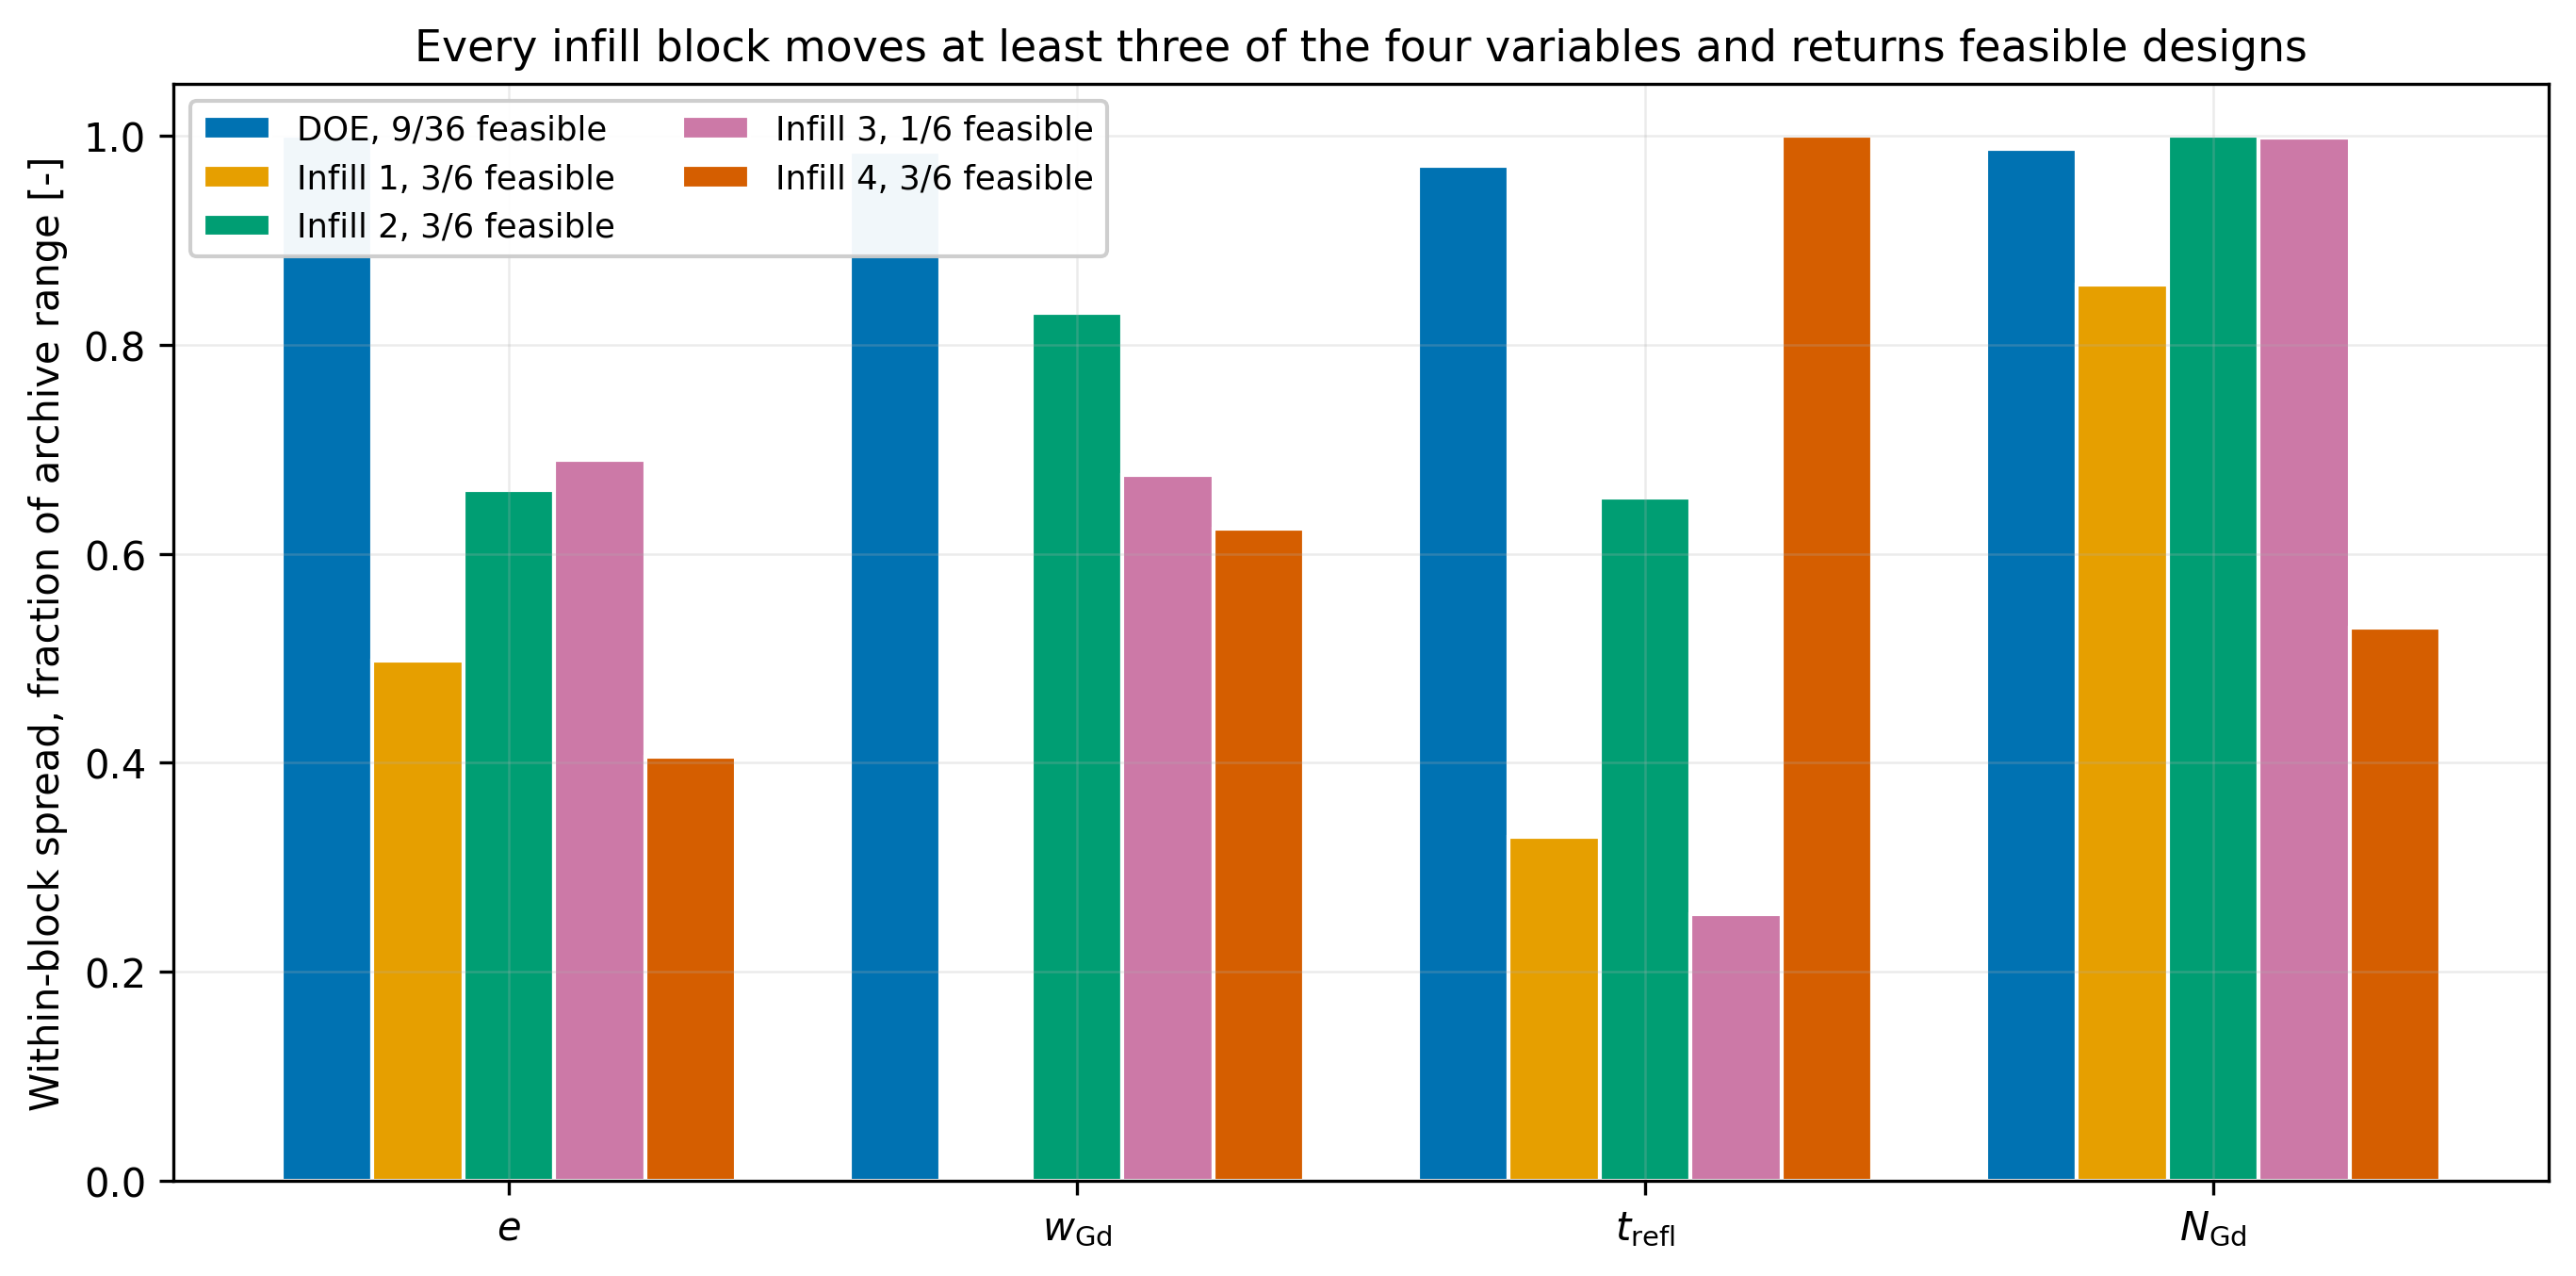
\includegraphics[width=\linewidth]{images/c8_infill_diversity}
  \caption{Within-block spread of each design variable in Campaign 8.}
  \label{fig:c8-diversity}
\end{figure}

\begin{figure}[htbp]
  \centering
  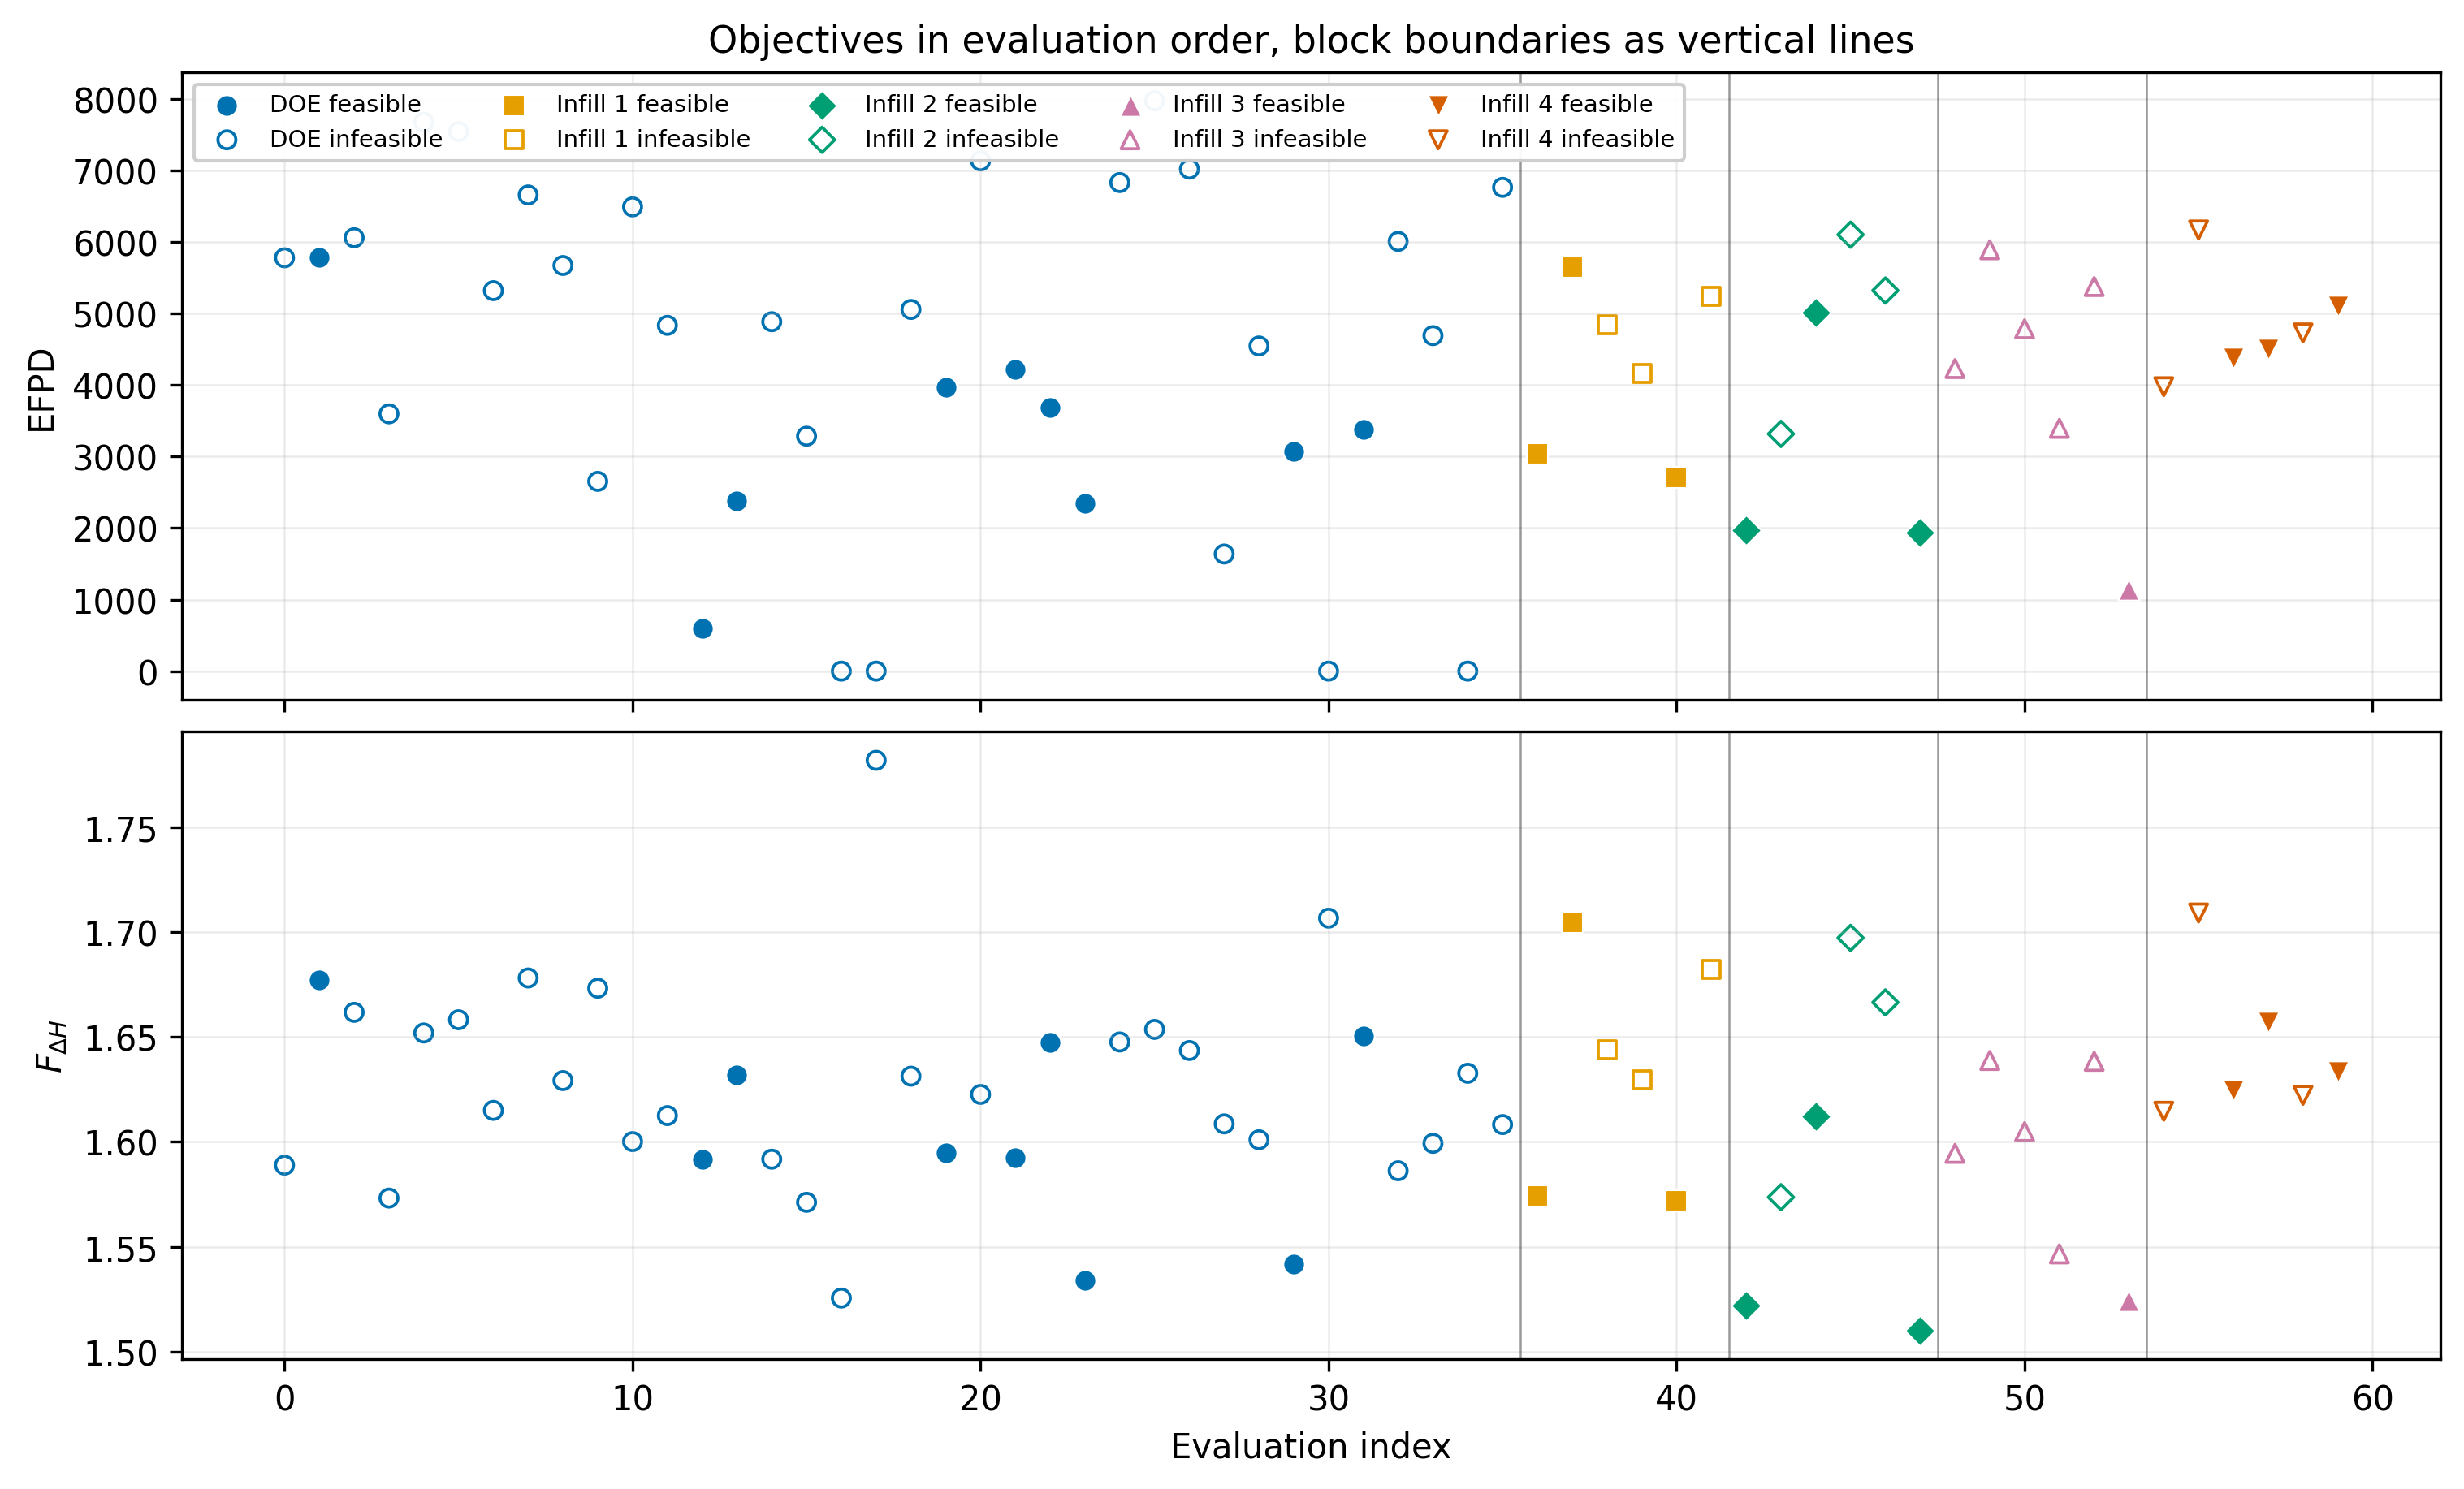
\includegraphics[width=\linewidth]{images/c8_trajectory}
  \caption{Campaign 8 objectives in evaluation order.}
  \label{fig:c8-trajectory}
\end{figure}

The convergence record is honest rather than complete. The hypervolume
gained \SI{2.87}{\%} in block 2 and then \SI{0.00}{\%} and
\SI{0.18}{\%} in blocks 3 and 4. Under the rule of
Section~\ref{sec:res-c6-blocks}, three consecutive gains below one per
cent with no censored design on the front, the campaign is one block
short of a formal stop. Unlike Campaign 7, the flat blocks here are not
acquisition failures: their designs are diverse and land on the
constraint boundary where the surrogate expects the front to be
(Figure~\ref{fig:c8-plane}). The front is therefore reported as
converged at the resolution the frozen reference can see, with the
stated caveat. In Figure~\ref{fig:c8-plane} the four-bank state on the
left is the constraint and the two-bank state on the right is recorded
only. The two-bank reading is subcritical only below an unrodded
eigenvalue of about 1.07.

\subsection{Feasibility and the binding constraint}
\label{sec:res-c8-screens}

Of the 60 designs, 19 are feasible, \SI{31.7}{\%}, with 9 of 36 in the
design of experiments. Table~\ref{tab:c8-nesting} gives the census and
Figure~\ref{fig:c8-activity} the activity per block. The nesting of
Campaign 7 is reversed: the ceiling never rejects a design that the
control screen accepts. The control screen
rejects 35 designs and is the dominant constraint in every block. No
design fails the peaking bound, the enrichment cap or the vessel fit.

\begin{table}[htbp]
  \centering
  \caption{Constraint census of Campaign 8 and the joint activity of the two reactivity screens.}
  \label{tab:c8-nesting}
  \begin{tabular}{lc}
    \toprule
    Outcome & Designs \\
    \midrule
    Fail $g_\mathrm{ctrl}$                          & 35 \\
    Fail $g_{k\max}$ at 1.166                       & 23 \\
    Fail $g_{k\max}$ and pass $g_\mathrm{ctrl}$     &  0 \\
    Fail $g_\mathrm{ctrl}$ and pass $g_{k\max}$     & 12 \\
    Fail $g_{k\min}$                                &  6 \\
    Feasible on all six                             & 19 \\
    Feasible and controllable with two banks        &  4 \\
    \bottomrule
  \end{tabular}
\end{table}

\begin{figure}[htbp]
  \centering
  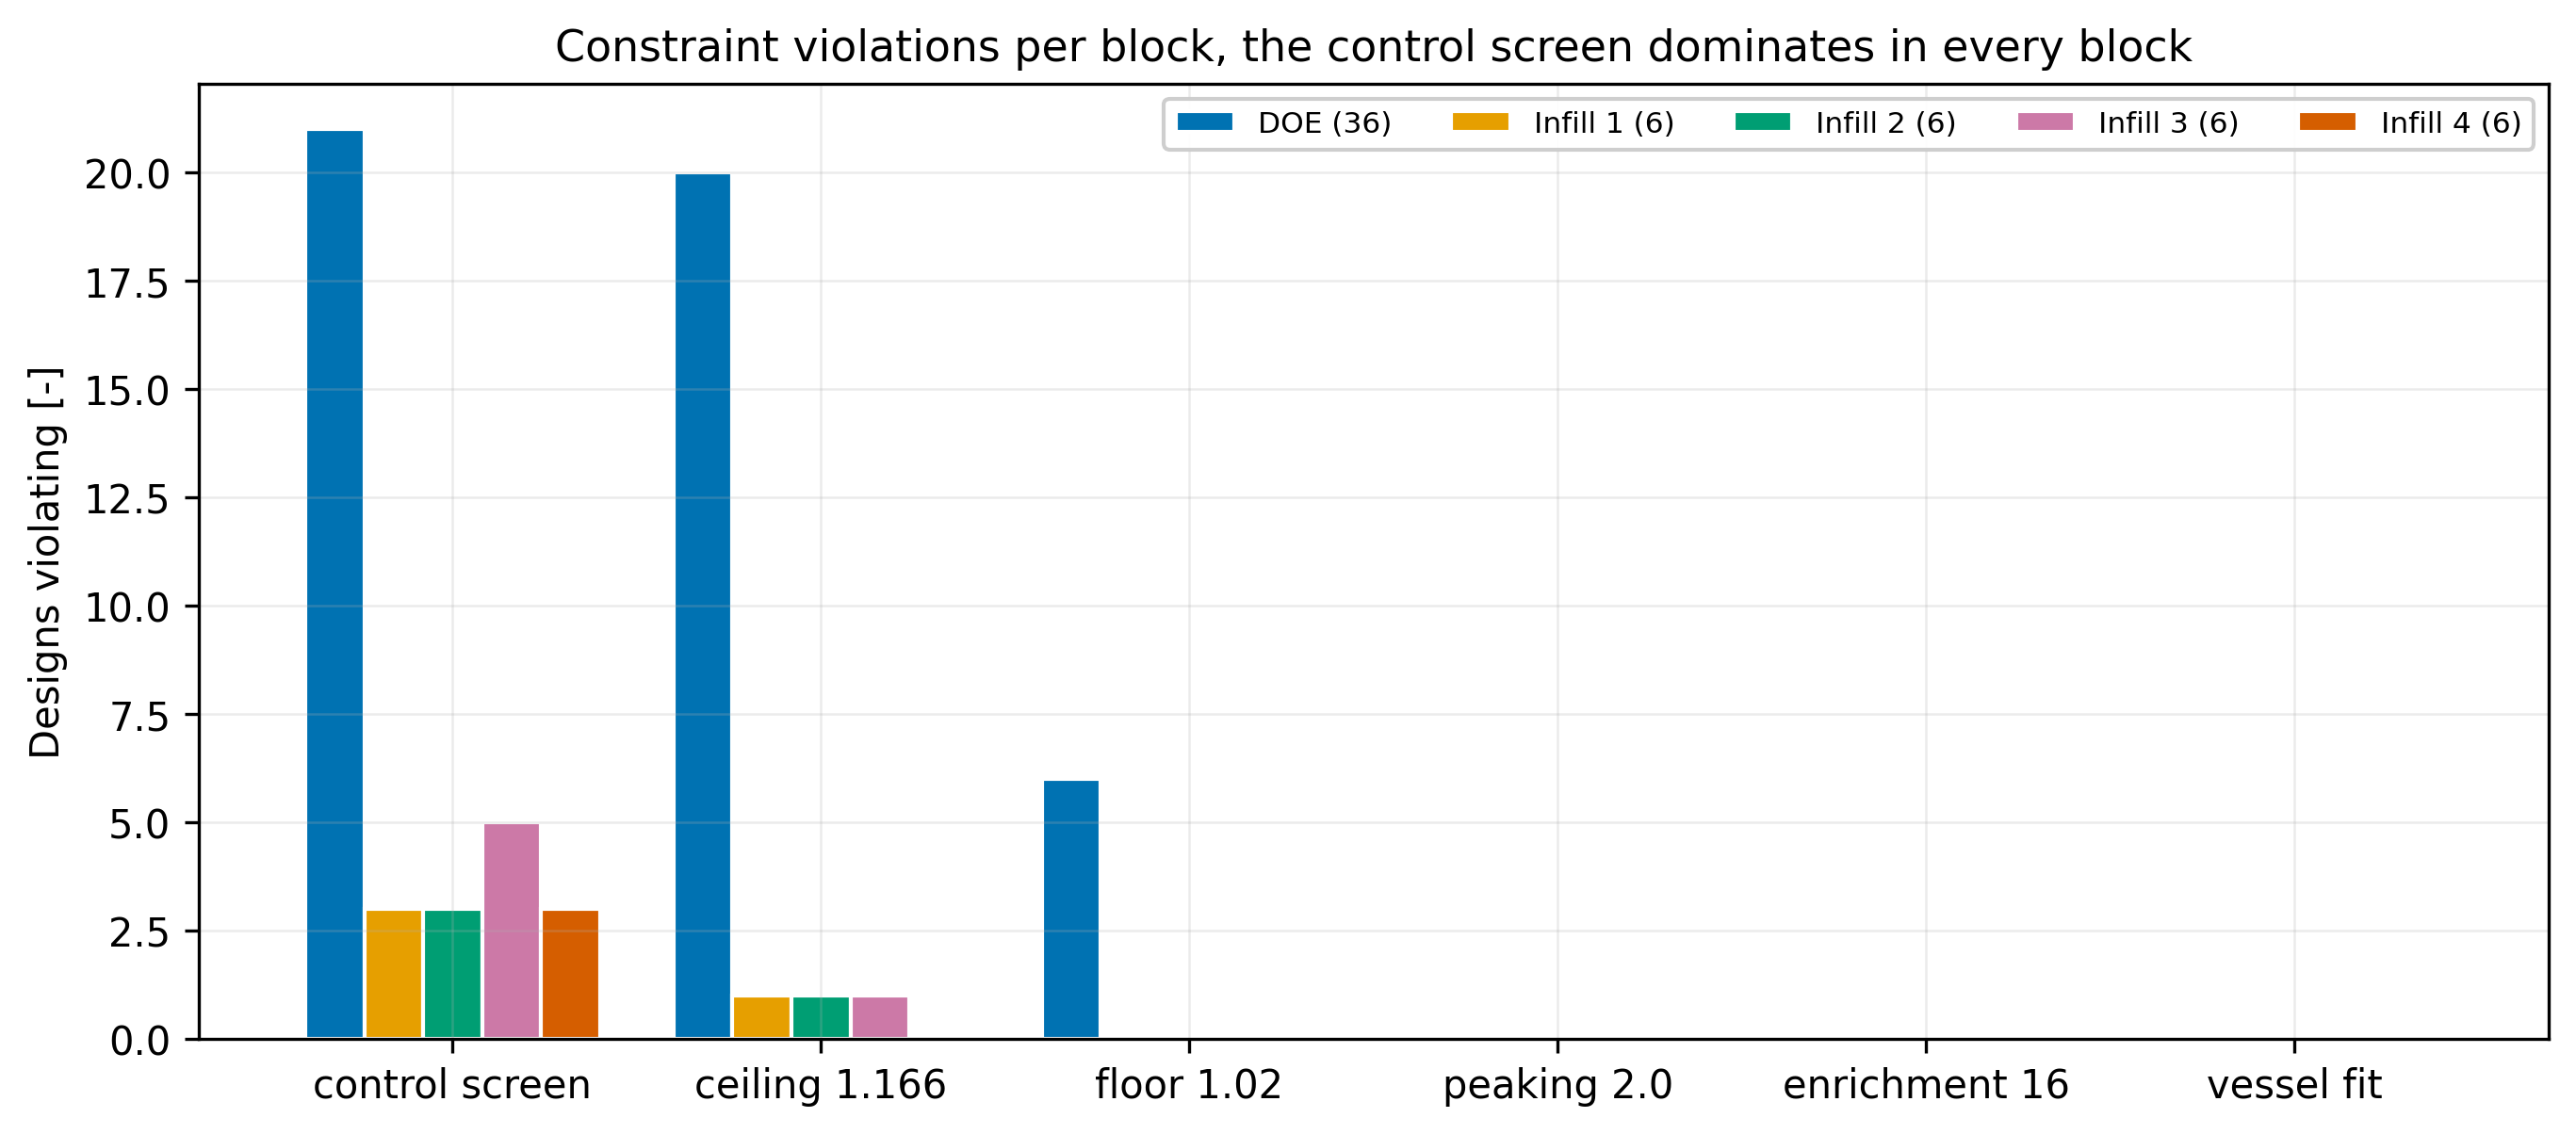
\includegraphics[width=\linewidth]{images/c8_constraint_activity}
  \caption{Campaign 8 constraint violations per block.}
  \label{fig:c8-activity}
\end{figure}

\begin{figure}[htbp]
  \centering
  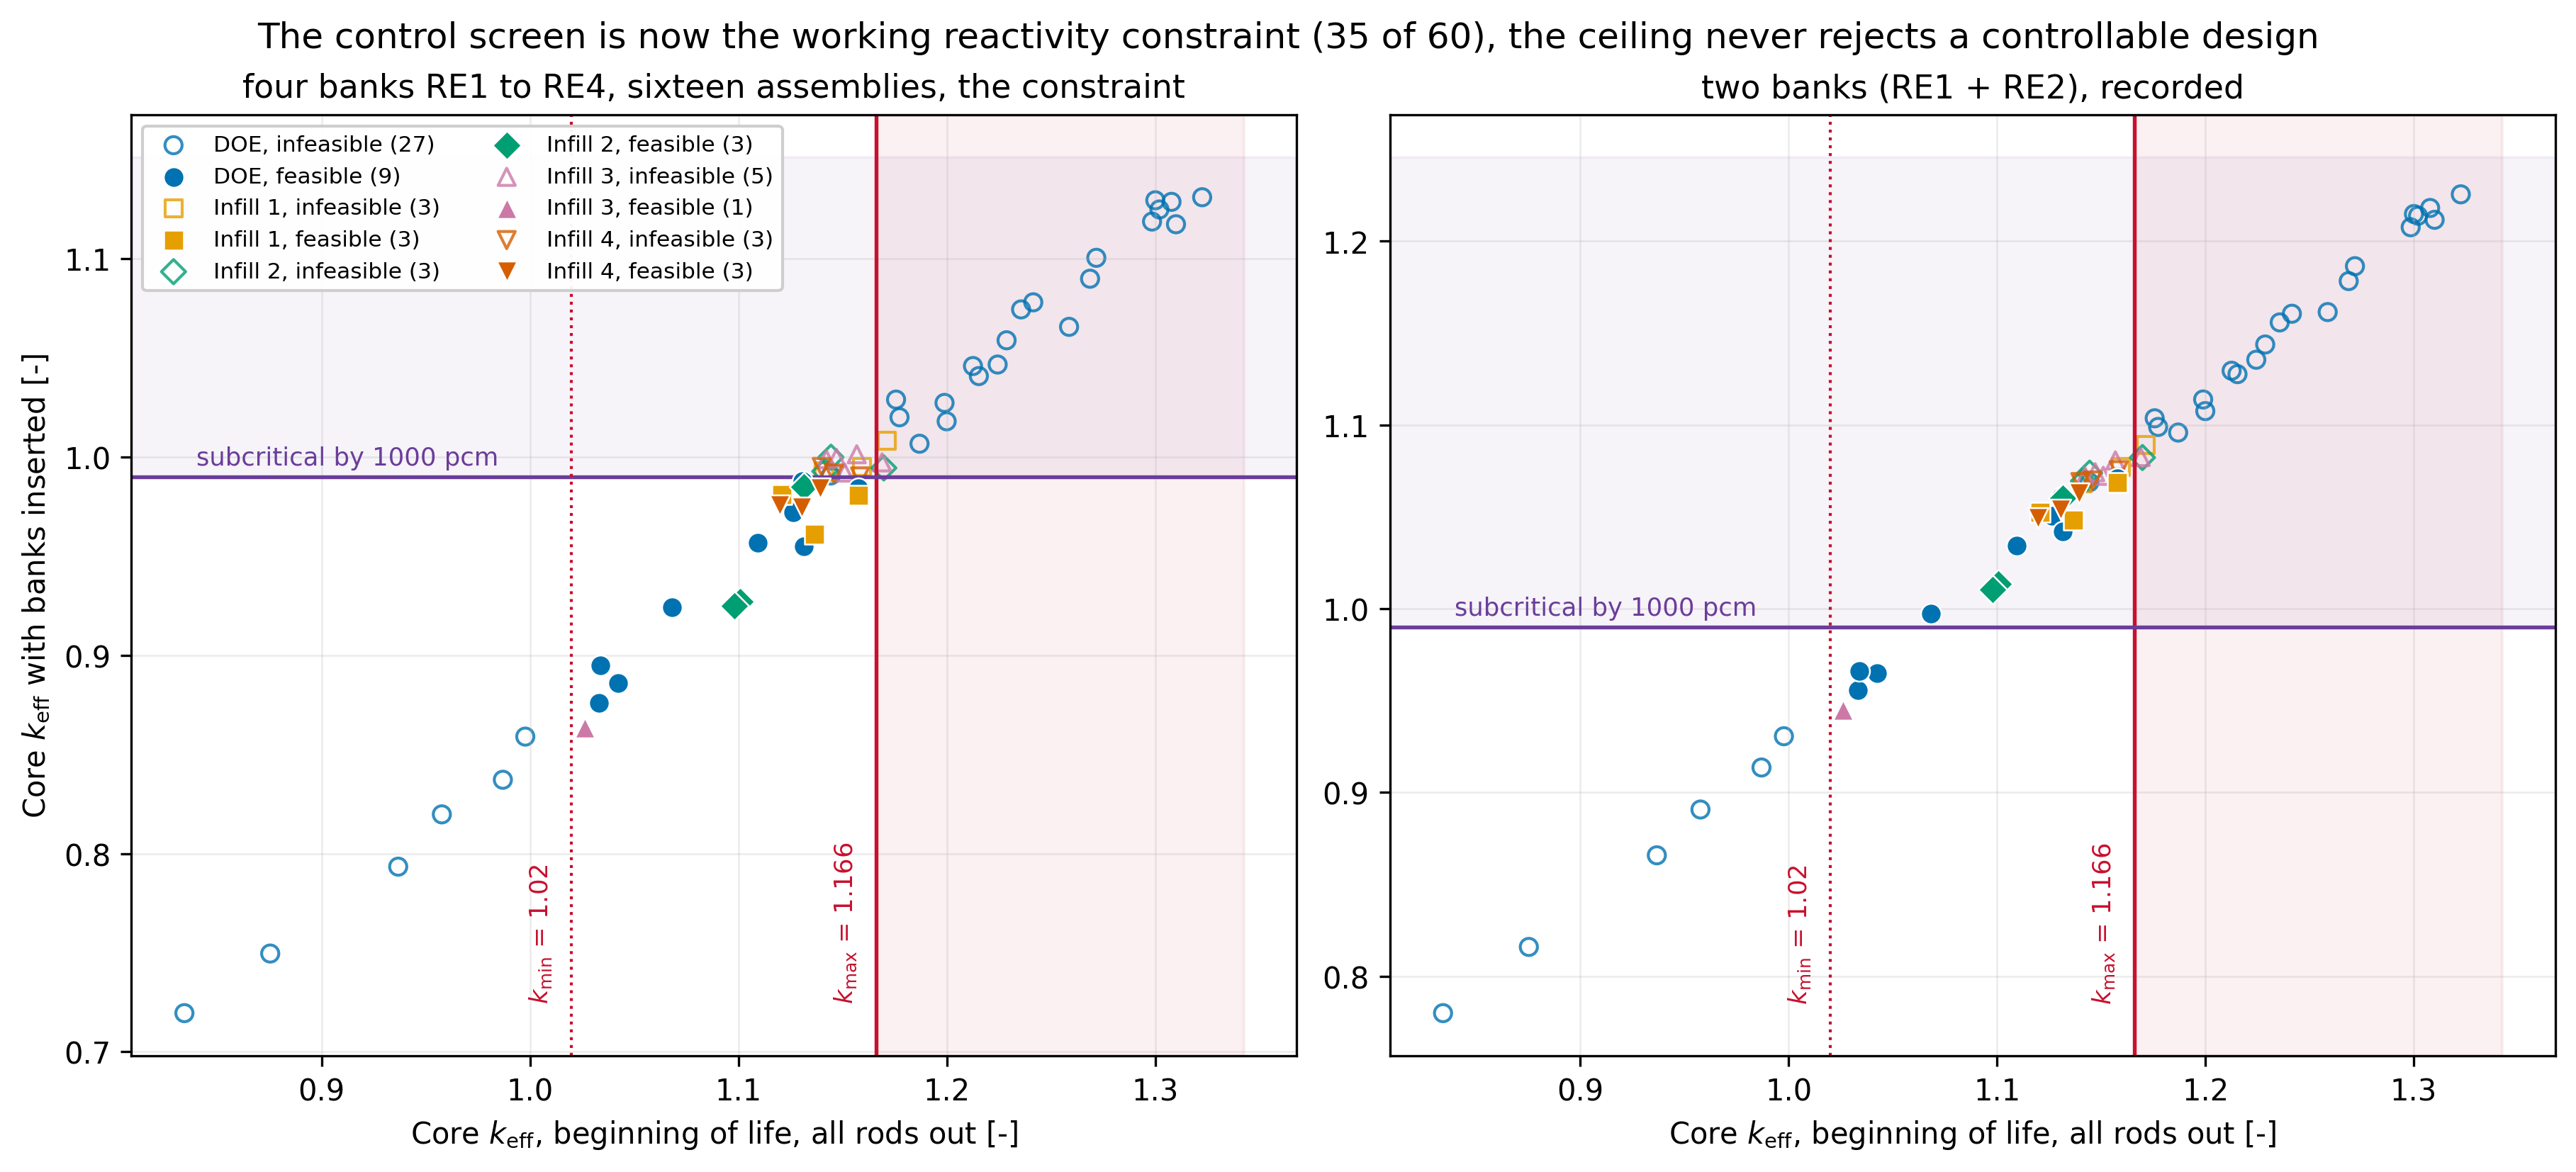
\includegraphics[width=\linewidth]{images/c8_ctrl_plane}
  \caption{Campaign 8 unrodded core eigenvalue against the eigenvalue with four banks inserted, left, and with two banks inserted, right.}
  \label{fig:c8-plane}
\end{figure}

This is the constraint architecture the campaign was built to produce.
Not one design fails the derived ceiling while passing the measured
screen, so the ceiling of 1.166 did no work, and twelve designs pass
the ceiling while failing the screen, so the screen did all of it. The
twelve are the long-cycle designs, from 3977 to 6169 EFPD, and they
fail by 17 to \SI{1135}{pcm} in the rodded eigenvalue. Two of them,
designs 54 and 11, fail by 17 and \SI{63}{pcm}, within the statistical
resolution of a single core solve, and are treated as marginal rather
than rejected in Section~\ref{sec:res-c8-limits}.

The bank worths of Equation~\eqref{eq:bank-worth} run from
\num{11466} to \SI{19313}{pcm} for the four banks and from
\num{5429} to \SI{9841}{pcm} for the first two, with the ratio between
\num{0.473} and \num{0.511} on all 60 designs and a mean of
\num{0.496}. Figure~\ref{fig:c8-worths} shows both against the two
absorber variables. At fixed pitch the gadolinium pin count is the
single driver, correlating at $-0.73$ with both worths, and the
concentration adds a weaker $-0.39$.

\begin{figure}[htbp]
  \centering
  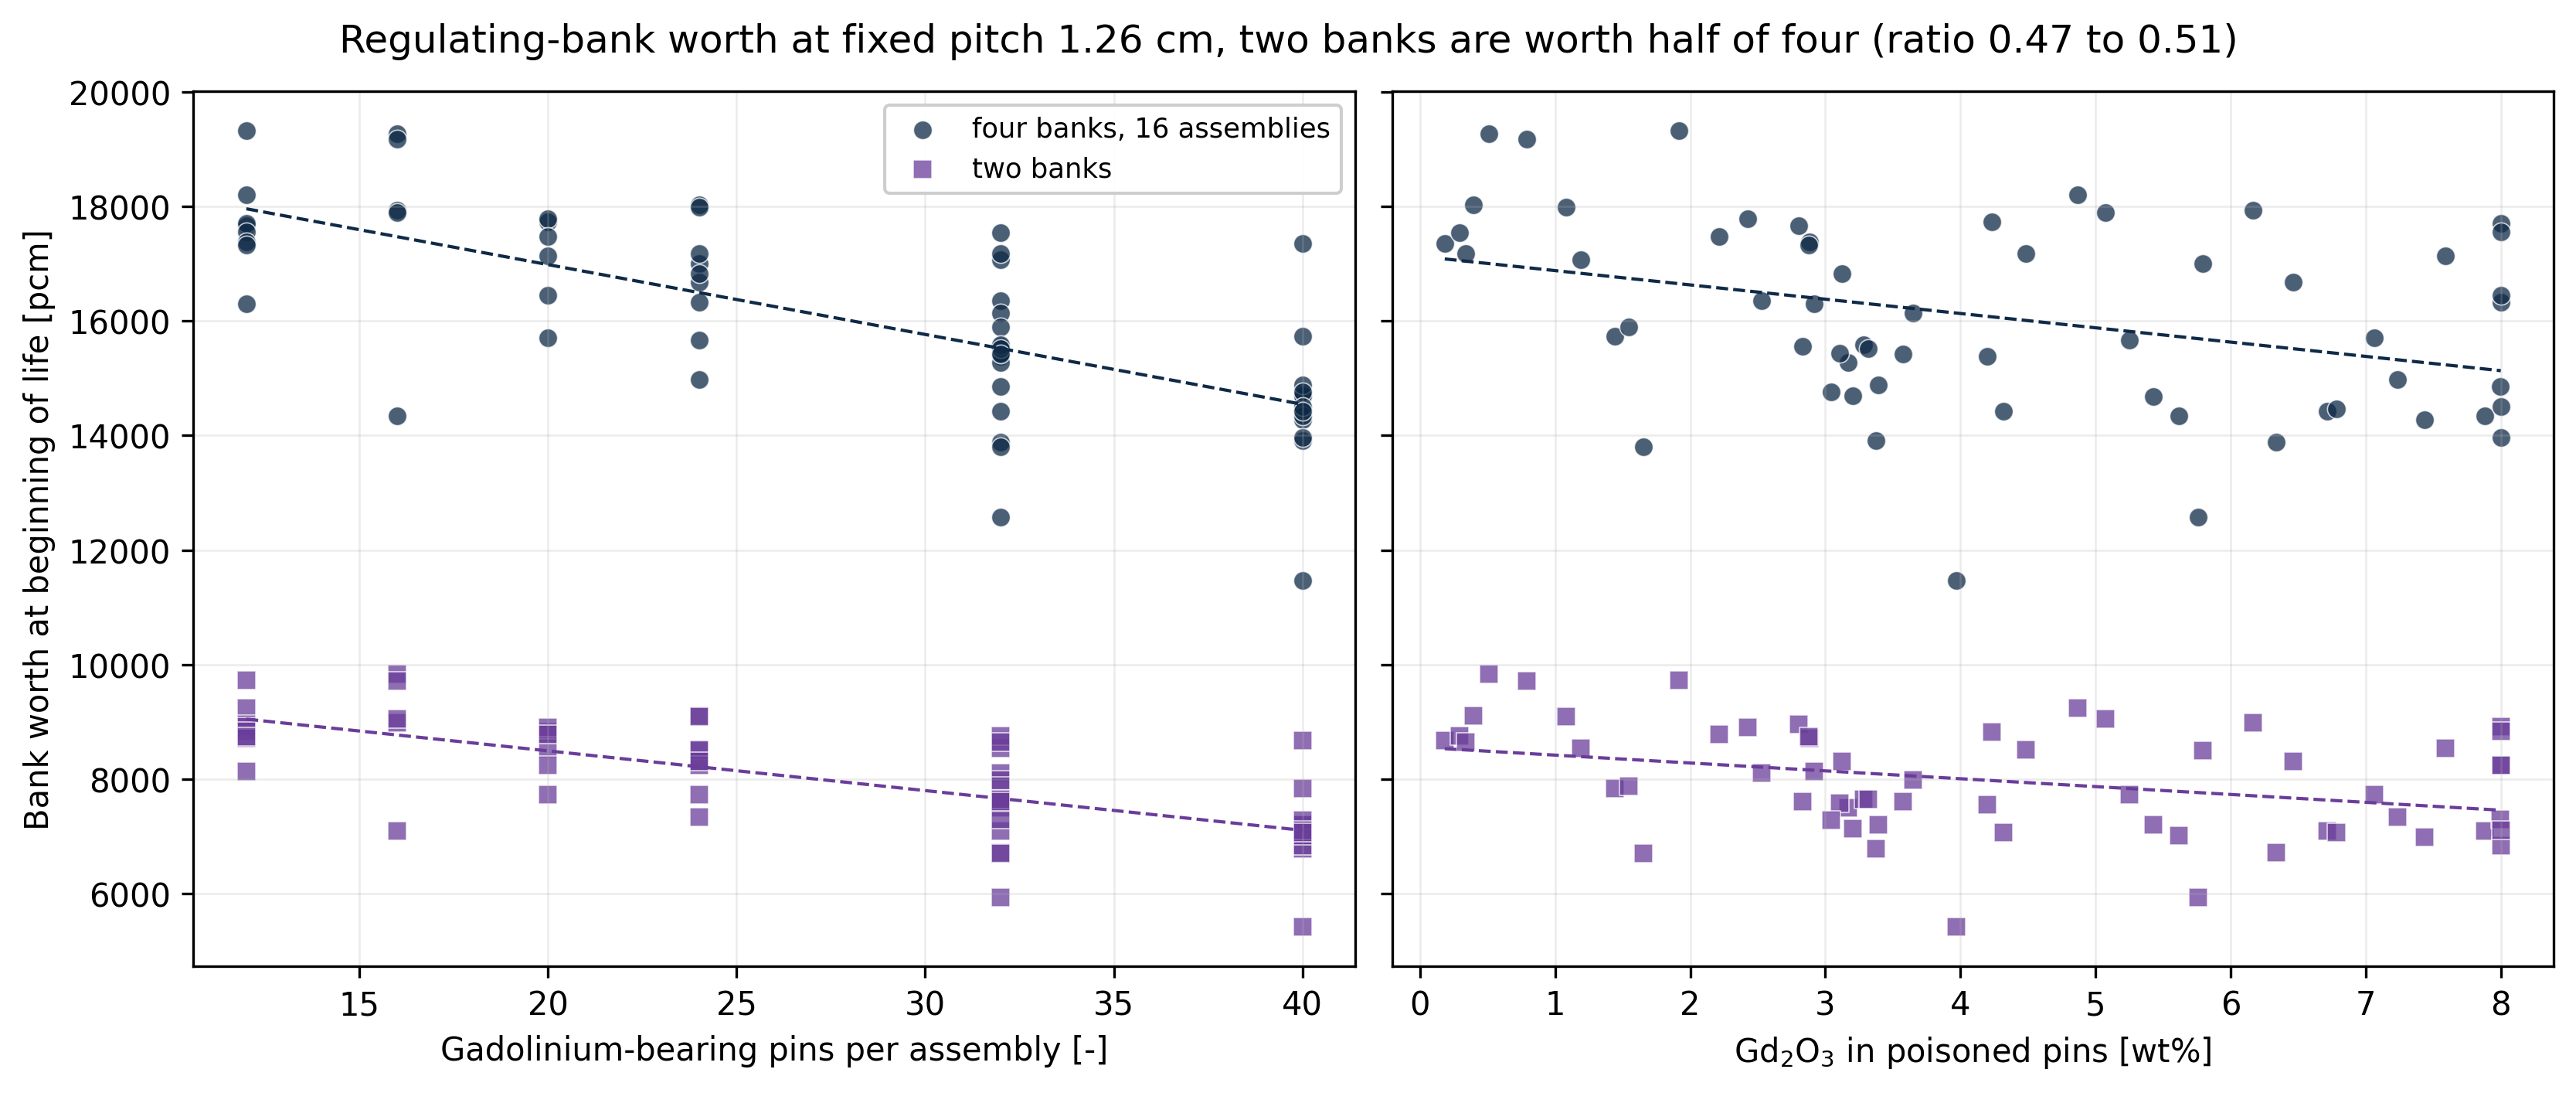
\includegraphics[width=\linewidth]{images/c8_worths}
  \caption{Regulating-bank worth at fixed pitch, four banks and two banks, against the gadolinium pin count and concentration.}
  \label{fig:c8-worths}
\end{figure}

The two-bank ceiling follows from the smallest two-bank worth as the
four-bank ceiling did in Section~\ref{sec:meth-ctrl}.

\begin{equation}
k_{\max}^{(2)} = (1 - \Delta\rho_\mathrm{op}) + \rho_\mathrm{bank}^{(2)}
\label{eq:two-bank-ceiling}
\end{equation}

\noindent where the symbols have the following meaning.

\begin{itemize}
  \item $k_{\max}^{(2)}$ is the highest unrodded eigenvalue that the
        first two banks alone can hold down at the margin,
        dimensionless.

  \item $\Delta\rho_\mathrm{op}$ is the operating margin, \num{0.01}.

  \item $\rho_\mathrm{bank}^{(2)}$ is the two-bank worth in units of
        $k$, \num{0.0543} to \num{0.0984} across the archive, median
        \num{0.0793}.
\end{itemize}

The median gives 1.069 and the minimum 1.044. The two-bank window
above the floor of 1.02 is therefore about \SI{5000}{pcm} wide, against
\SI{13000}{pcm} for four banks, and it holds four of the nineteen
feasible designs.

\subsection{The front}
\label{sec:res-c8-front}

The feasible non-dominated set holds eight designs, from 1941 to 5782
EFPD and from $F_{\Delta H}$ 1.510 to 1.677. Table~\ref{tab:c8-front}
lists them and Figure~\ref{fig:c8-pareto} places every design in the
objective plane with its block. In the table the ring enrichments are
the as-built centre, middle and periphery values, the excess is the
beginning-of-life reactivity at \SI{1000}{ppm} that the rods must hold,
and the peaking factor is given with all rods out ($F$), with two banks
in ($F_2$) and with four banks in ($F_{16}$). In the figure filled
markers are feasible, purple rings mark the four feasible designs
controllable with the first two banks alone, and the vertical dotted
lines are five calendar years at capacity factors of 0.5 and 0.8. Four
front designs come from the
design of experiments, three from infill block 2 and one from block 4.
The discharge screen of \SI{75}{MWd/kgHM} is inactive on the front,
whose highest end-of-cycle burnup is \SI{57.7}{MWd/kgHM}, and no
design is censored.

\begin{table}[htbp]
  \centering
  \small
  \caption[The Campaign 8 front]{The Campaign 8 front.}
  \label{tab:c8-front}
  \setlength{\tabcolsep}{3.4pt}
  \begin{tabular}{ccccccccccc}
    \toprule
    Design & EFPD & rings & $w_\mathrm{Gd}$ & $n_\mathrm{Gd}$ &
      $t_\mathrm{refl}$ & $k^\mathrm{core}$ & excess & $F$ & $F_{2}$ &
      $F_{16}$ \\
    {[--]} & [d] & [wt\%] & [wt\%] & [rods] & [cm] & [--] & [pcm] &
      [--] & [--] & [--] \\
    \midrule
    47 & 1941 & 3.16, 3.93, 5.05  & 2.88 & 12 & 4.29 & 1.098 &  8930 & 1.510 & 1.991 & 2.314 \\
    42 & 1968 & 3.20, 3.97, 5.11  & 2.88 & 12 & 3.76 & 1.101 &  9154 & 1.522 & 1.997 & 2.264 \\
    23 & 2346 & 3.56, 4.42, 5.68  & 2.80 & 12 & 4.81 & 1.132 & 11626 & 1.534 & 1.968 & 2.356 \\
    29 & 3070 & 4.25, 5.27, 6.79  & 0.18 & 40 & 4.69 & 1.158 & 13627 & 1.542 & 1.935 & 2.218 \\
    21 & 4221 & 5.63, 6.98, 8.99  & 3.11 & 32 & 4.92 & 1.126 & 11220 & 1.592 & 1.934 & 2.194 \\
    44 & 5019 & 6.65, 8.25, 10.61 & 3.20 & 40 & 5.33 & 1.132 & 11631 & 1.612 & 1.996 & 2.177 \\
    59 & 5104 & 6.73, 8.35, 10.75 & 4.32 & 40 & 5.66 & 1.120 & 10701 & 1.634 & 1.998 & 2.214 \\
     1 & 5782 & 7.94, 9.85, 12.68 & 7.43 & 40 & 3.94 & 1.131 & 11554 & 1.677 & 2.007 & 2.210 \\
    \bottomrule
  \end{tabular}
\end{table}

\begin{figure}[htbp]
  \centering
  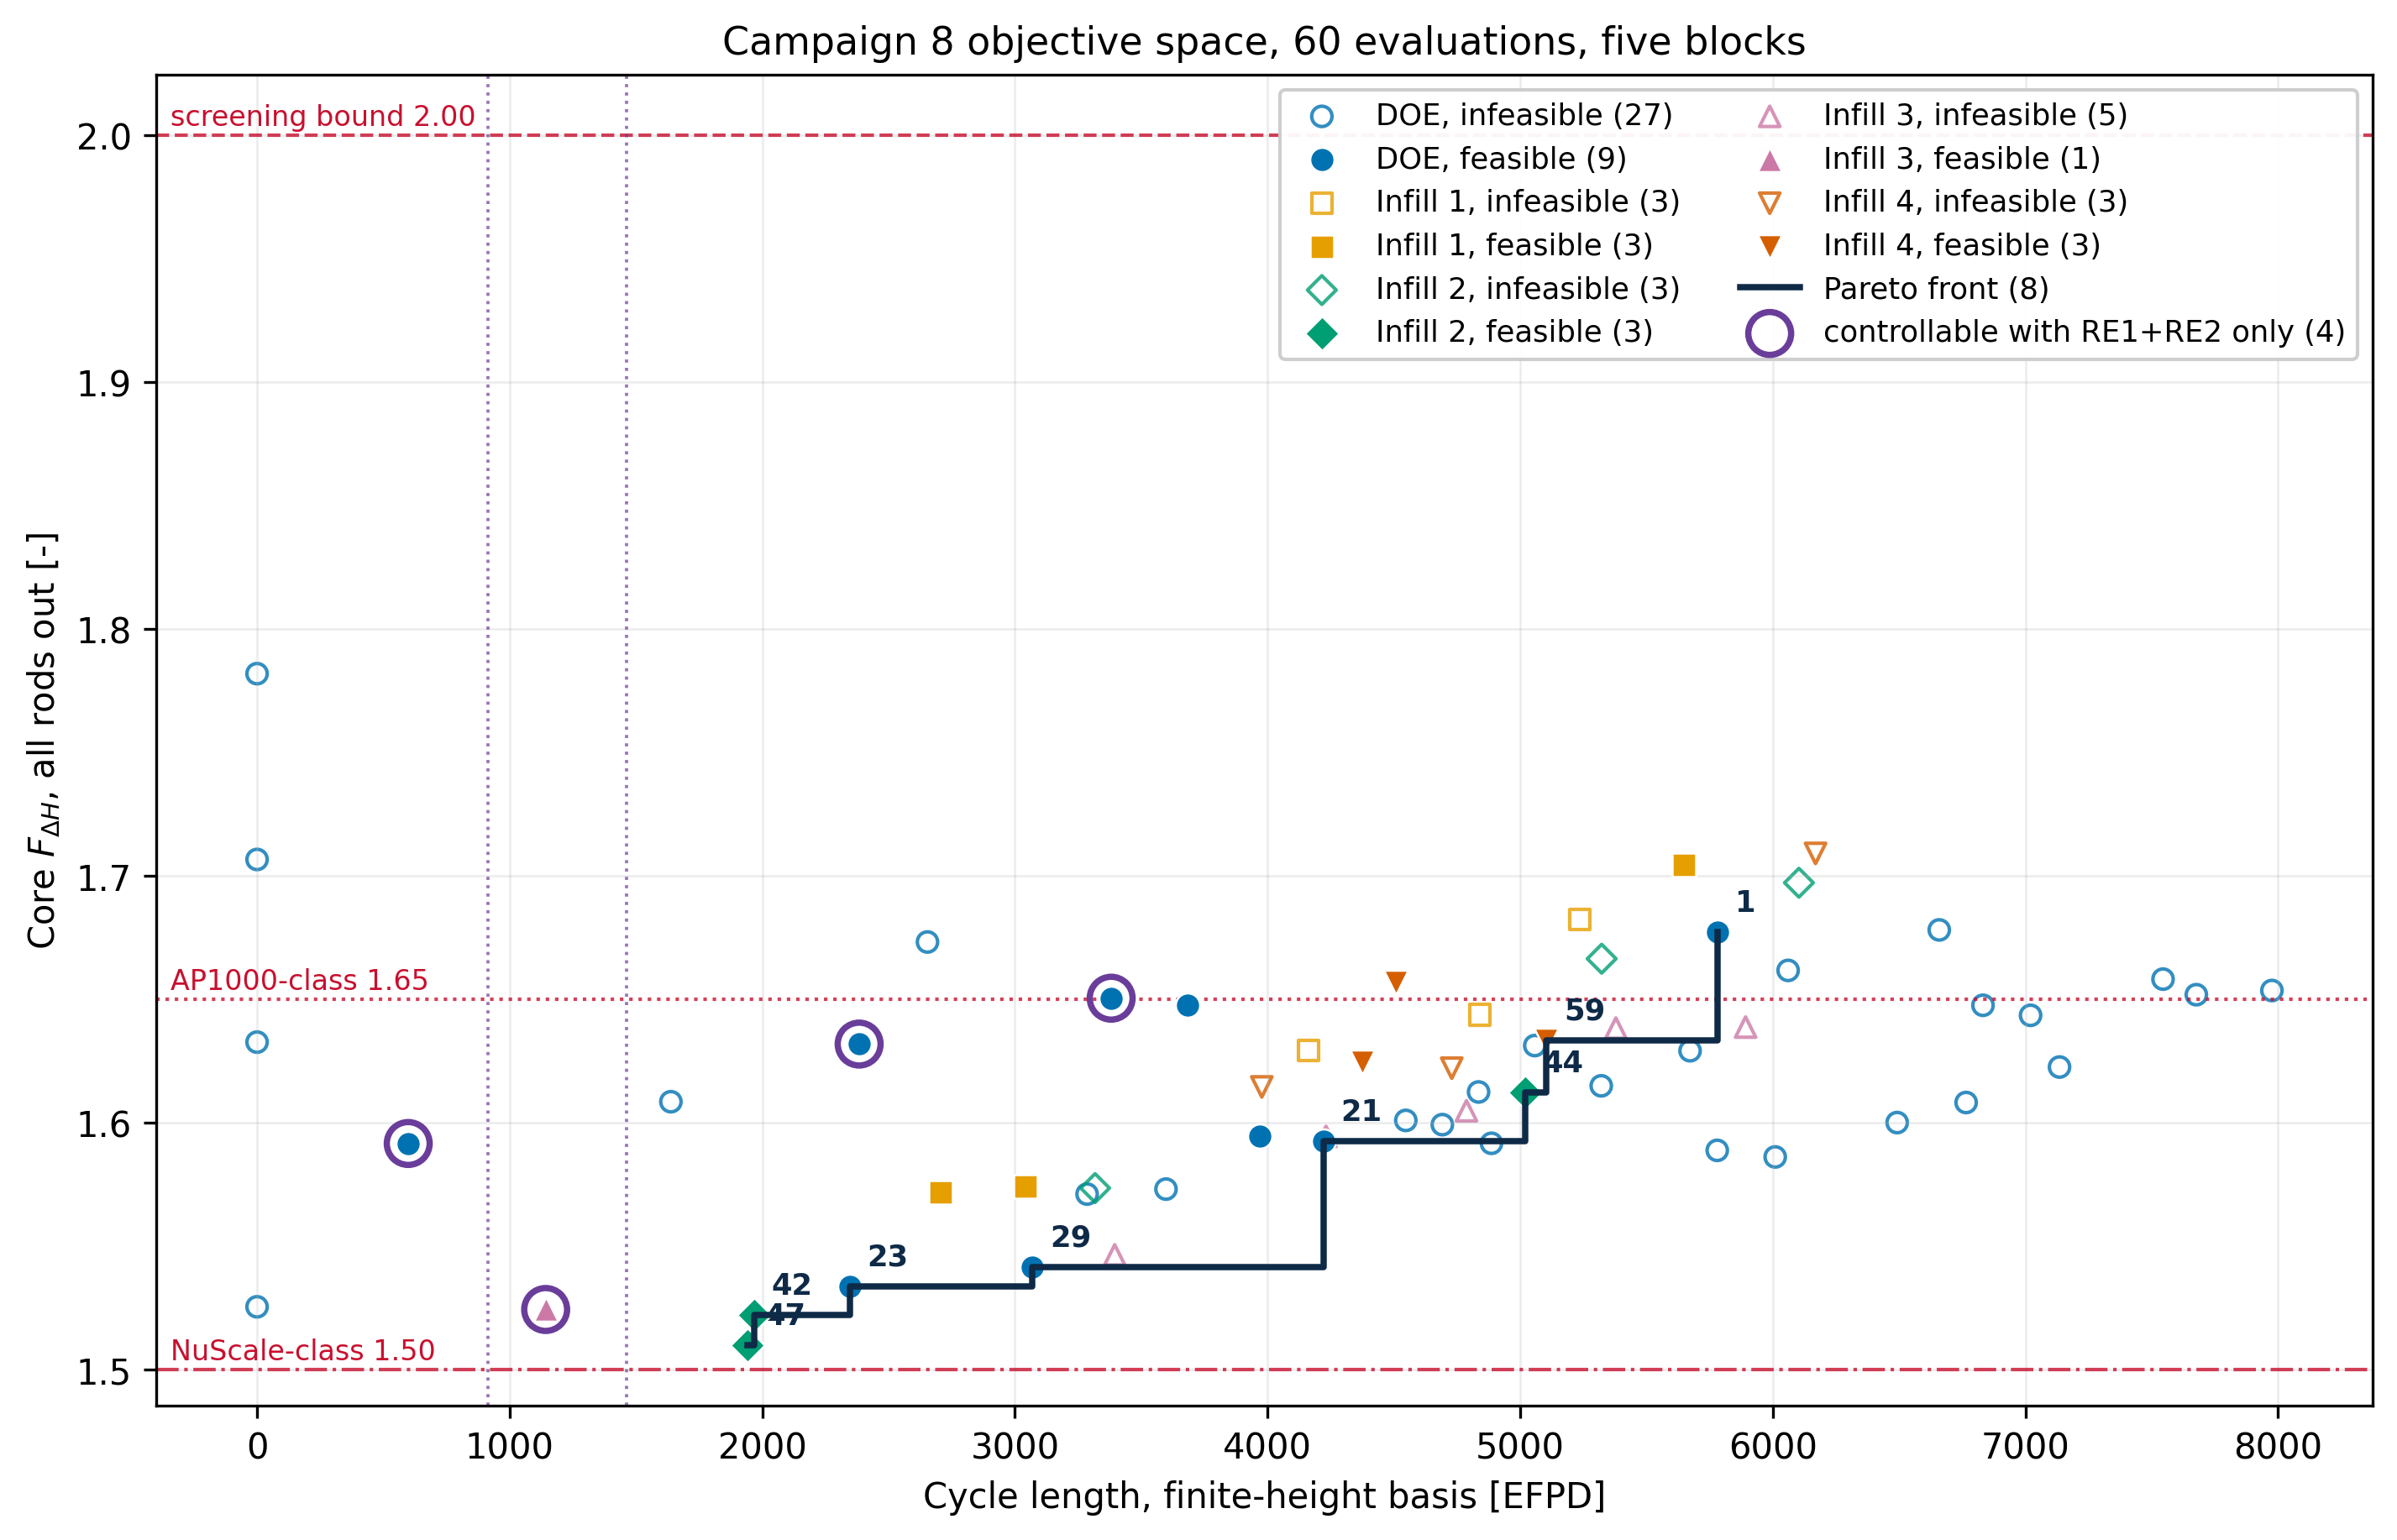
\includegraphics[width=\linewidth]{images/c8_pareto}
  \caption{Campaign 8 objective space with the five blocks distinguished.}
  \label{fig:c8-pareto}
\end{figure}

Three features of the front carry into the candidate discussion.

\begin{enumerate}
  \item The peaking floor did not rise. The pre-registered expectation
        was a floor near 1.60, on the argument that the low-peaking end
        of the Campaign 7 front lived at thick reflectors that the fixed
        pitch cannot accommodate. The Campaign 8 floor is 1.510, at
        design 47, and it is reached by a different route: a low uniform
        enrichment with twelve poisoned pins and a short cycle. The
        reflector lever was removed and the enrichment lever took its
        place. Peaking correlates at $+0.82$ with enrichment over the
        feasible set (Figure~\ref{fig:c8-influence}).

  \item Every front design sits on the control boundary. The unrodded
        eigenvalues run from 1.098 to 1.158, and the rodded eigenvalues
        from 0.925 to 0.988, so the beginning-of-life excess that the
        four banks must hold lies between \num{8930} and
        \SI{13627}{pcm} with the soluble boron already in the coolant.
        Design 29, with \SI{0.18}{wt\%} gadolinia on forty pins, is
        effectively unpoisoned and carries the largest excess.

  \item The two-bank peaking of every front design is 1.93 to 2.01.
        With only RE1 and RE2 inserted the front sits on the screening
        bound, and with all four banks it exceeds it by 0.18 to 0.36
        (Figure~\ref{fig:c8-split}). The rodded peaking is a property of
        the map, not of the design: over all 60 designs the two-bank
        value spans only 1.82 to 2.35.
\end{enumerate}

\begin{figure}[htbp]
  \centering
  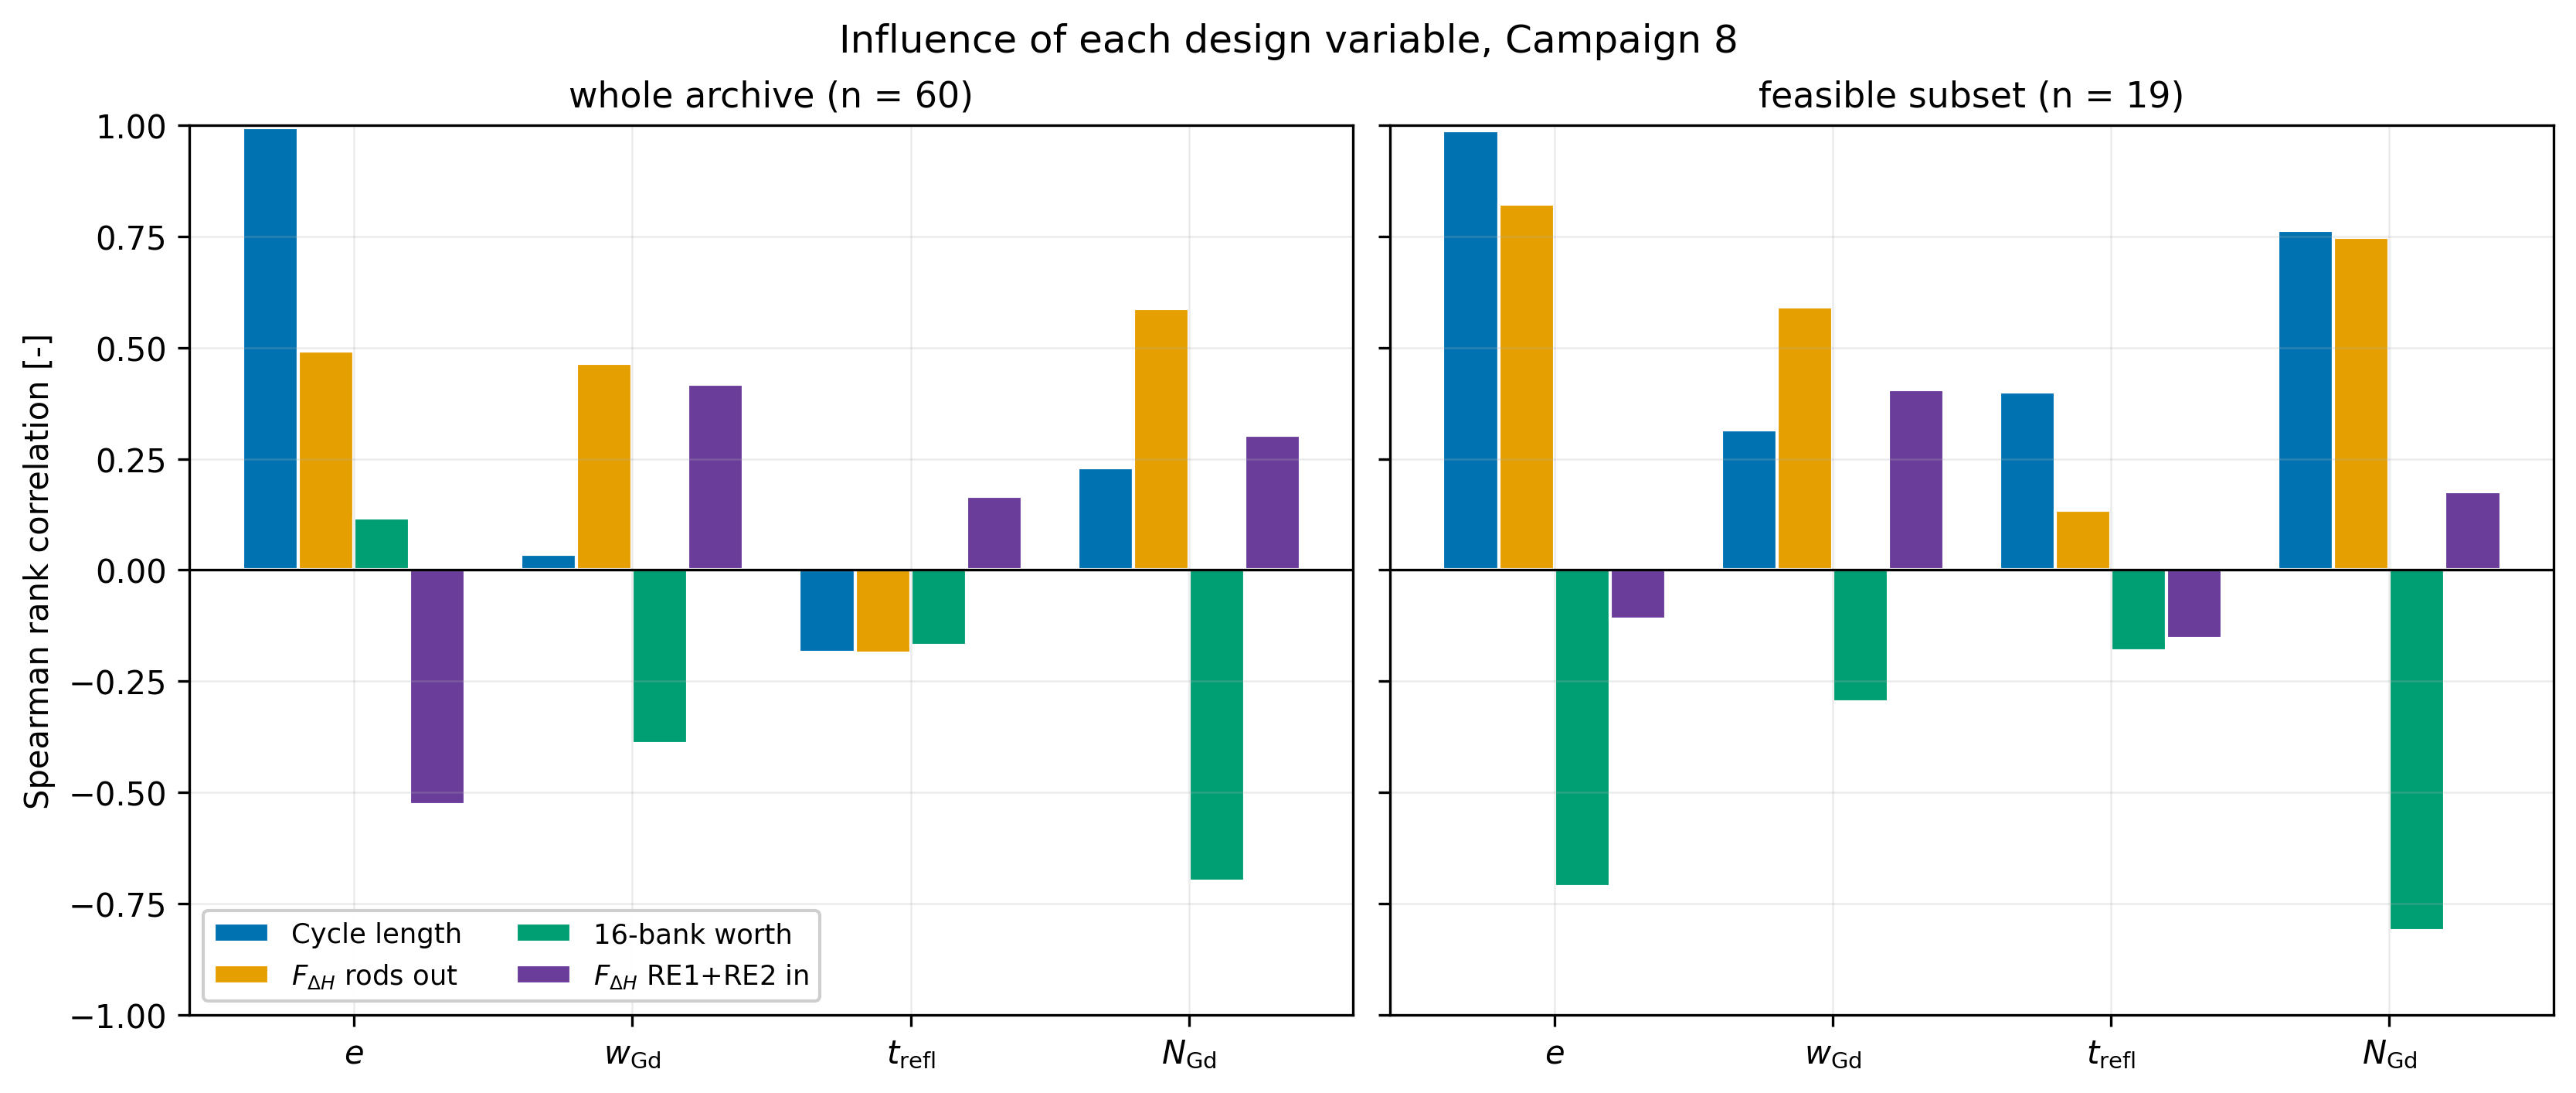
\includegraphics[width=\linewidth]{images/c8_vars_influence}
  \caption{Spearman rank correlation of each design variable with the
  objectives, the four-bank worth and the two-bank peaking, over the
  archive and over the feasible subset.}
  \label{fig:c8-influence}
\end{figure}

\begin{figure}[htbp]
  \centering
  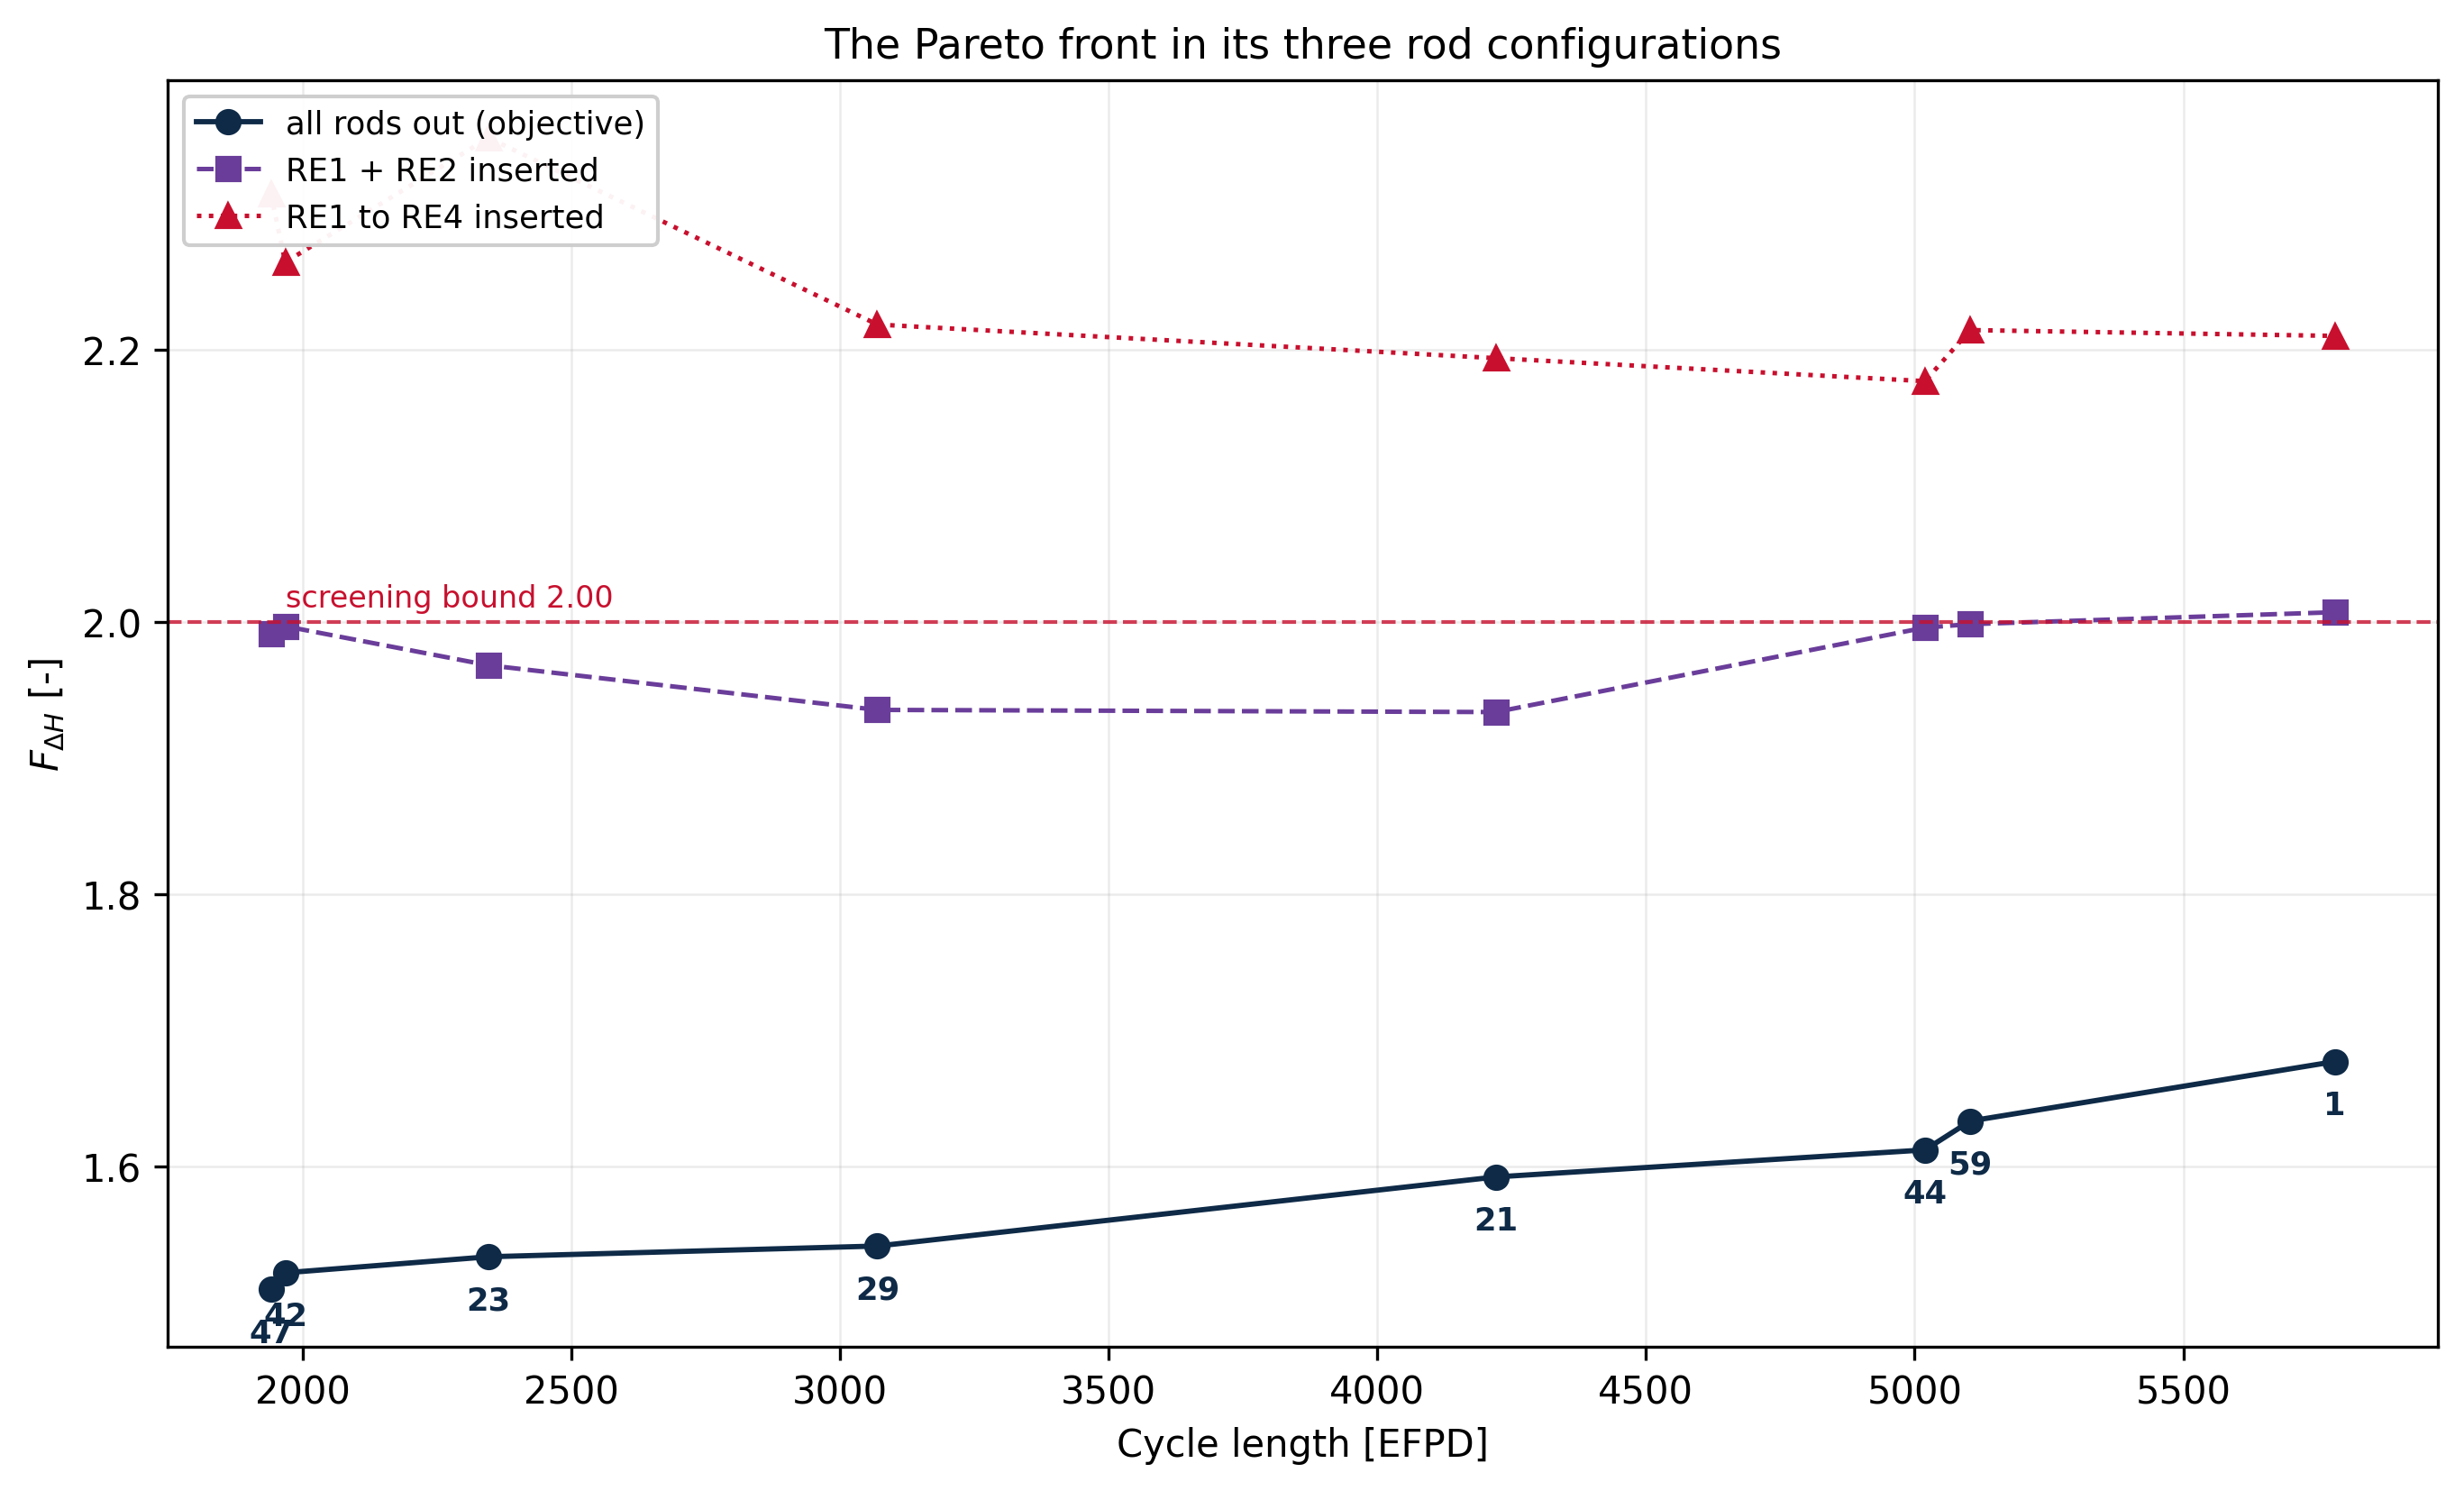
\includegraphics[width=0.95\linewidth]{images/c8_front_split}
  \caption{The Campaign 8 front in its three rod configurations.}
  \label{fig:c8-split}
\end{figure}

% ---------------------------------------------------------------------
%  Validation of the framework on the Campaign 8 archive.
%  Protocol in Section \ref{sec:validation-framework}.
%  Tables generated by c8_surrogate_cv.py (c8_cv_table.tex) and
%  c8_front_stability.py (c8_stab_table.tex).
% ---------------------------------------------------------------------

\subsection{Cross-validation of the surrogate}
\label{sec:res-c8-cv}

The protocol of Section~\ref{sec:validation-surrogate} is applied to the
60 archived designs. Table~\ref{tab:c8-cv-loo} and
Figure~\ref{fig:c8-cv-loo} report the leave-one-out
result for the two objectives and for the two eigenvalues that carry the
controllability screen of Section~\ref{sec:meth-ctrl}. The exercise is a
post-processing step on the archive and costs no transport time.

\begin{table}[htbp]
  \centering
  \small
  \setlength{\tabcolsep}{4.5pt}
  \begin{threeparttable}
  \caption[Leave-one-out validation of the surrogate]{Leave-one-out cross-validation of the Gaussian Process surrogate on the Campaign 8 archive.}
  \label{tab:c8-cv-loo}
  \begin{tabular}{llrrrrrrr}
    \toprule
    Quantity & Subset & $n$ & RMSE & $R^2$ & $\rho_\mathrm{S}$ & Cov.\ $1\sigma$ & Cov.\ $2\sigma$ & $s_z$ \\
    \midrule
    Cycle length [EFPD] & all & 60 & 220 & 0.988 & 0.997 & 0.77 & 0.87 & 1.63 \\
     & feasible & 19 & 145 & 0.990 & 0.988 & 0.74 & 0.89 & 1.81 \\
    $F_{\Delta H}$ & all & 60 & 0.0287 & 0.690 & 0.830 & 0.65 & 0.93 & 1.26 \\
     & feasible & 19 & 0.0227 & 0.829 & 0.900 & 0.63 & 0.89 & 1.26 \\
    $k_\mathrm{core}$ & all & 60 & 0.0151 & 0.978 & 0.967 & 0.67 & 0.97 & 1.11 \\
     & feasible & 19 & 0.0111 & 0.930 & 0.875 & 0.63 & 1.00 & 0.98 \\
    $k_\mathrm{RE}$ & all & 60 & 0.0110 & 0.985 & 0.961 & 0.65 & 0.97 & 1.11 \\
     & feasible & 19 & 0.0081 & 0.959 & 0.923 & 0.68 & 1.00 & 1.02 \\
    \bottomrule
  \end{tabular}
  \begin{tablenotes}\footnotesize
    \item RMSE is the root mean square error of the held-out prediction. $R^2$ is the coefficient of determination. $\rho_\mathrm{S}$ is the Spearman rank correlation between predicted and true values. Cov.\ $1\sigma$ and Cov.\ $2\sigma$ are the fractions of true values inside the one-sigma and two-sigma predictive intervals, with nominal values 0.683 and 0.954. $s_z$ is the standard deviation of the standardised residual, equal to 1 for a calibrated predictor.
    \item Source: c8\_surrogate\_cv.py on the archive of 60 designs, of which 19 are feasible.
  \end{tablenotes}
  \end{threeparttable}
\end{table}

Four readings follow directly from the table.

\begin{enumerate}
  \item The cycle length is the best predicted quantity. Its coefficient
        of determination is 0.988 over the archive and 0.990 over the
        feasible subset, and the held-out root mean square error falls
        from 220 to 145 EFPD when the fit is scored on the feasible
        designs alone.

  \item The peaking factor is the worst predicted quantity. Its
        coefficient of determination is 0.690 over the archive and 0.829
        over the feasible subset. The held-out root mean square error of
        0.0287 over the archive is of the same order as the spacing of
        the front members of Table~\ref{tab:c8-front}, whose adjacent
        designs differ by 0.008 to 0.051 in $F_{\Delta H}$.

  \item The two eigenvalues are predicted to 0.0151 and 0.0110 in $k$
        over the archive, that is \num{1510} and \SI{1100}{pcm} read as
        $10^{5}\,\Delta k$. Their rank correlations, 0.967 and 0.961,
        are the quantity the acquisition actually uses, because the
        margin rule of Section~\ref{sec:meth-acq} ranks candidates
        rather than reading their absolute values.

  \item The predictive intervals are too narrow on the objectives and
        close to correct on the eigenvalues. The one-sigma coverage lies
        between 0.63 and 0.77 against a nominal 0.683, and the
        standardised residual has a standard deviation of 1.63 and 1.81
        on the cycle length, against 1 for a calibrated predictor. The
        two eigenvalues have $s_z$ between 0.98 and 1.11.
\end{enumerate}

\begin{figure}[htbp]
  \centering
  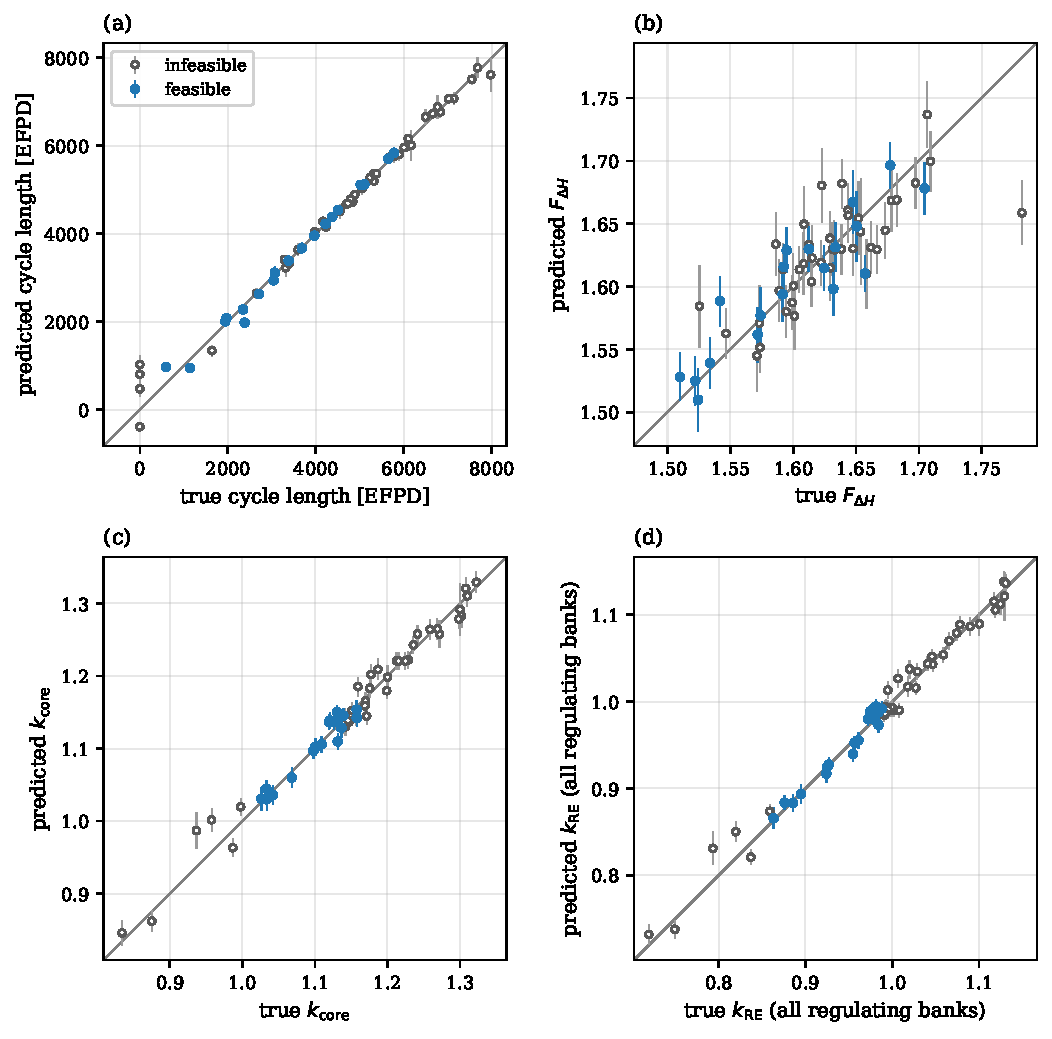
\includegraphics[width=\linewidth]{images/c8_cv_loo}
  \caption[Leave-one-out predictions against transport truth]{Held-out
  prediction against transport truth for the two objectives and the two
  eigenvalues of the controllability screen. Error bars are one
  predictive standard deviation.}
  \label{fig:c8-cv-loo}
\end{figure}

Figure~\ref{fig:c8-cv-loo} shows where the residuals of
Table~\ref{tab:c8-cv-loo} sit. The two eigenvalues and the cycle length
follow the diagonal over their whole range. The exception is the
short-cycle end of the archive, where the held-out prediction departs
from the truth by several hundred effective full-power days and is
negative for one design, since a Gaussian Process is not constrained to
return non-negative outputs. Those designs are the ones that never reach
the reactivity target and are rejected long before the front is formed.

The leave-one-out result measures the surrogate at the end of the
campaign. The walk-forward result of
Figure~\ref{fig:c8-cv-walkforward} measures it at decision time, on the
six designs of each infill block, with the surrogate fitted only on the
evaluations that preceded the block.

\begin{figure}[htbp]
  \centering
  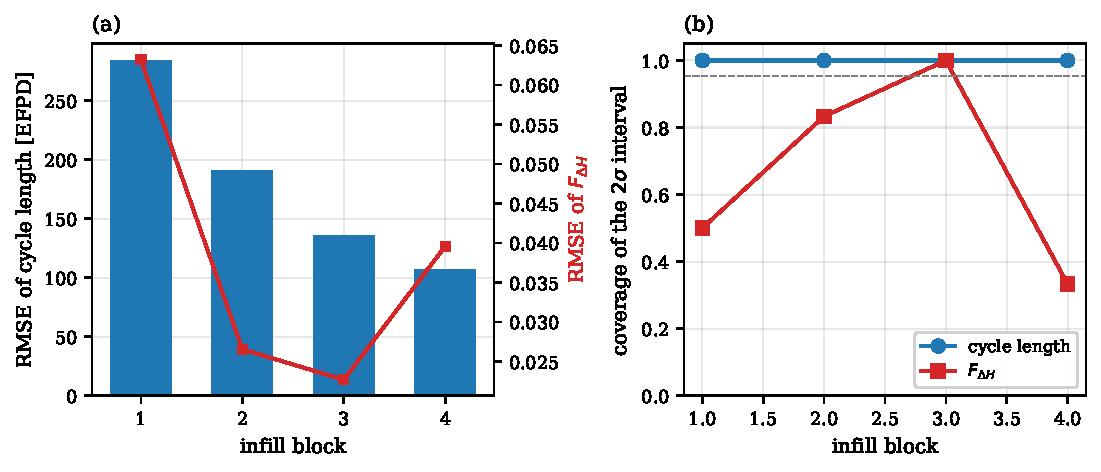
\includegraphics[width=\linewidth]{images/c8_cv_walkforward}
  \caption[Walk-forward accuracy and coverage per infill block]{Block
  root mean square error and two-sigma coverage of the surrogate at
  decision time, per infill block. The dashed line in panel (b) is the
  nominal coverage of 0.954.}
  \label{fig:c8-cv-walkforward}
\end{figure}

Three readings follow from the walk-forward record.

\begin{enumerate}
  \item The cycle-length prediction improved monotonically as the
        archive grew. The block root mean square error fell from
        \SI{285}{EFPD} at infill block 1 to \num{191}, \num{136} and
        \SI{107}{EFPD} at blocks 2, 3 and 4.

  \item The peaking prediction did not. Its block root mean square error
        fell from 0.063 to 0.027 and 0.022 at blocks 2 and 3, and then
        rose to 0.040 at block 4.

  \item At decision time the intervals are conservative on the cycle
        length and erratic on the peaking factor. The two-sigma coverage
        of the cycle length is 1.00 at every block, above the nominal
        0.954, while that of the peaking factor is 0.50, 0.83, 1.00 and
        0.33. Each block holds six designs, so the coverage is quantised
        in steps of one sixth and these four values carry little
        resolution.
\end{enumerate}

The walk-forward surrogate is fitted on fewer designs than the
leave-one-out surrogate and therefore returns wider predictive
intervals. This is why the cycle length appears over-confident in
Table~\ref{tab:c8-cv-loo}, with a two-sigma coverage of 0.87, and
under-confident in Figure~\ref{fig:c8-cv-walkforward}, with a coverage
of 1.00. The two measurements are not in conflict, because they score
different fits.

An over-confident cycle-length surrogate has no direct effect on the
feasibility margin of the acquisition, because the margin rule of
Section~\ref{sec:meth-acq} acts on the constraint surrogates and the
cycle length is an objective. The constraint eigenvalues
$k_\mathrm{core}$ and $k_\mathrm{RE}$ are the quantities whose
predictive standard deviations are multiplied by $\kappa$, and their
two-sigma coverage in Table~\ref{tab:c8-cv-loo} is 0.97 to 1.00, at or
above the nominal value, so the margin added during the campaign was
at least as wide as intended. The under-stated cycle-length
uncertainty enters only the uncertainty ranking of the candidates,
where a narrower band on that output gives the objective slightly
less weight in the choice of the infill batch.

\subsection{Stability of the front}
\label{sec:res-c8-stability}

The protocol of Section~\ref{sec:validation-front} is applied to the
eight members of Table~\ref{tab:c8-front}.
Table~\ref{tab:c8-front-stability} reports, for each member, the
evaluation at which it entered the feasible non-dominated set, its
exclusive hypervolume contribution and its probability of remaining
non-dominated under the Monte Carlo noise of the transport solves.

\begin{table}[htbp]
  \centering
  \begin{threeparttable}
  \caption[Stability of the Campaign 8 front]{Entry, exclusive hypervolume contribution and noise robustness of the Campaign 8 front members.}
  \label{tab:c8-front-stability}
  \begin{tabular}{rrrrrr}
    \toprule
    Design & Cycle [EFPD] & $F_{\Delta H}$ & Entered at & Excl.\ HV [\%] & $P$(front) \\
    \midrule
    47 & 1941 & 1.5099 & 48 & 0.1 & 0.80 \\
    42 & 1968 & 1.5221 & 43 & 0.0 & 0.73 \\
    23 & 2346 & 1.5338 & 24 & 0.1 & 0.73 \\
    29 & 3070 & 1.5417 & 30 & 1.8 & 1.00 \\
    21 & 4221 & 1.5925 & 22 & 1.1 & 0.92 \\
    44 & 5019 & 1.6123 & 45 & 0.8 & 0.94 \\
    59 & 5104 & 1.6335 & 60 & 0.2 & 0.99 \\
    1 & 5782 & 1.6772 & 2 & 14.0 & 1.00 \\
    \bottomrule
  \end{tabular}
  \begin{tablenotes}\footnotesize
    \item Entered at is the evaluation count at which the design first became a member of the feasible non-dominated set and it was never displaced afterwards. Excl.\ HV is the hypervolume lost when the design alone is removed, as a percentage of the front hypervolume at the campaign reference point. $P$(front) is the probability that the design remains non-dominated when the objectives of every feasible design are perturbed by Gaussian Monte Carlo noise, with $\sigma_k = 44$\,pcm propagated to the cycle length and $\sigma_F = 0.01$ on $F_{\Delta H}$, over 5000 replicates.
  \end{tablenotes}
  \end{threeparttable}
\end{table}

Three readings follow directly from the table.

\begin{enumerate}
  \item The front was still growing when the campaign stopped. Design 59
        entered at evaluation 60, the last of the campaign, and no
        member was displaced afterwards. The hypervolume record of
        Section~\ref{sec:res-c8-blocks} reaches the same conclusion from
        a different quantity, namely that the campaign is one block
        short of a formal stop.

  \item One design carries the front. Design 1, the long-cycle extreme,
        holds \SI{14.0}{\%} of the front hypervolume exclusively,
        against \SI{1.8}{\%} for design 29 and \SI{1.1}{\%} for design
        21. The three lowest-peaking members, 47, 42 and 23, contribute
        \SI{0.1}{\%}, \SI{0.0}{\%} and \SI{0.1}{\%}, because each is
        nearly covered by its neighbours in the objective plane.

  \item The low-peaking end of the front is not resolved by the
        transport statistics. Under the noise model of
        Equation~\eqref{eq:val-sigma-cycle}, with
        $\sigma_k = \SI{44}{pcm}$ propagated to the cycle length and
        $\sigma_F = 0.01$ on the peaking factor, designs 47, 42 and 23
        remain non-dominated in 0.80, 0.73 and 0.73 of 5000 replicates,
        against 1.00 for designs 29 and 1. This quantifies the
        limitation stated in Section~\ref{sec:res-c8-limits}, that the
        ordering of the three lowest-peaking designs is not resolved.
\end{enumerate}

Figure~\ref{fig:c8-stab-chrono} gives the chronology of the set, with the
block boundaries dotted in panel~(a), and Figure~\ref{fig:c8-stab-robust}
its robustness.

\begin{figure}[htbp]
  \centering
  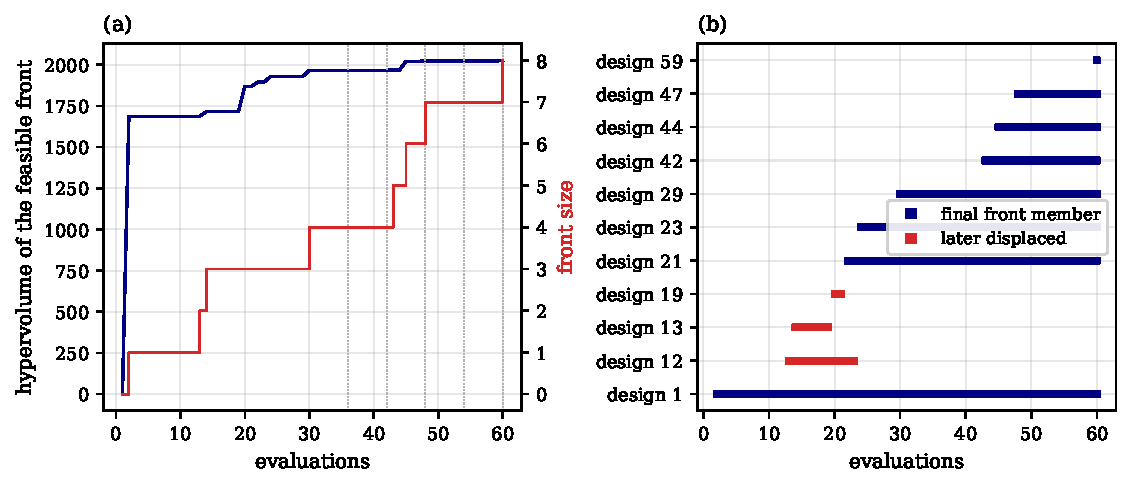
\includegraphics[width=\linewidth]{images/c8_stab_chrono}
  \caption[Chronology of the feasible non-dominated set]{Chronology of the Campaign 8 feasible front: hypervolume, front size and membership interval of every design, in evaluation order.}
  \label{fig:c8-stab-chrono}
\end{figure}

Figure~\ref{fig:c8-stab-chrono} adds the displacement record that
Table~\ref{tab:c8-front-stability} does not carry. Eleven designs
entered the feasible non-dominated set over the campaign and three of
them, designs 12, 13 and 19, were displaced later. All three entered and
left within the design of experiments. The four design of experiments
members that survived, designs 1, 21, 23 and 29, entered at evaluations
2, 22, 24 and 30 and were never displaced. The front size grew from one
member at evaluation 2 to eight at evaluation 60, and the last increment
is the entry of design 59.

\begin{figure}[htbp]
  \centering
  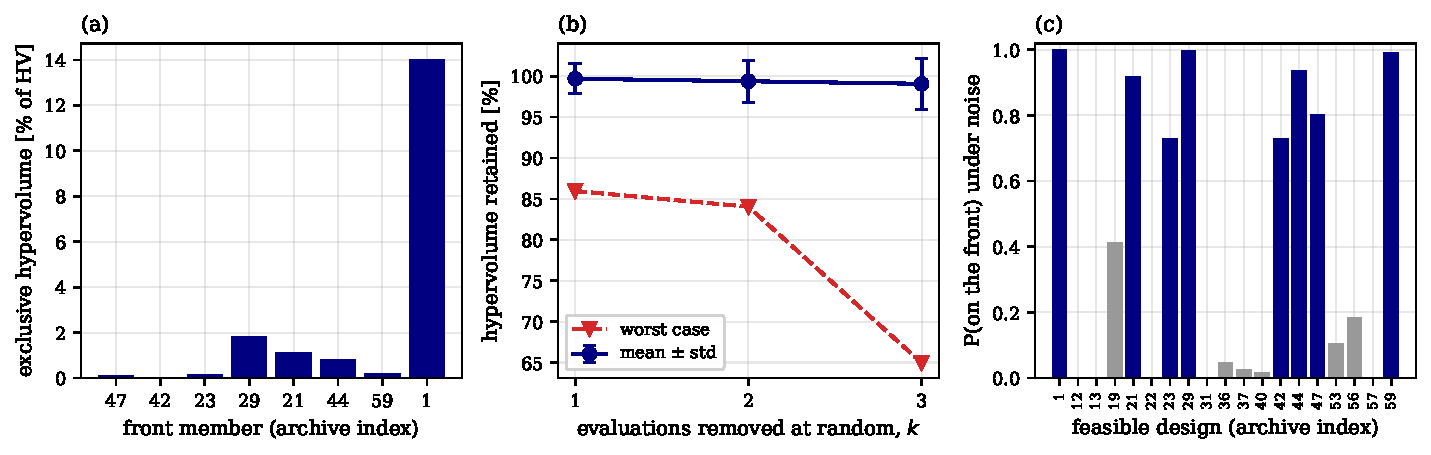
\includegraphics[width=\linewidth]{images/c8_stab_robust}
  \caption[Robustness of the Campaign 8 front]{Exclusive hypervolume of
  each front member, hypervolume retained after the random removal of
  evaluations, and the probability that each feasible design belongs to
  the front under Monte Carlo noise.}
  \label{fig:c8-stab-robust}
\end{figure}

Two further readings follow from Figure~\ref{fig:c8-stab-robust}.

\begin{enumerate}
  \item The front is robust to lost evaluations on average and fragile
        in the worst case. Removing one, two or three evaluations at
        random from the archive retains \SI{99.7}{\%}, \SI{99.4}{\%} and
        \SI{99.1}{\%} of the front hypervolume on average, while the
        worst case retains \SI{86.1}{\%}, \SI{84.2}{\%} and
        \SI{65.0}{\%}. The worst case at one removal is the loss of
        design 1, whose exclusive contribution is \SI{14.0}{\%}.

  \item Three designs that are not front members would become members
        under the same noise with non-negligible probability. Design 19
        reaches 0.41, design 56 reaches 0.19 and design 53 reaches 0.11.
        Design 19 is one of the three that were displaced during the
        design of experiments.
\end{enumerate}

A small exclusive hypervolume contribution and a membership probability
near unity are not in conflict. The first says that the design can be
removed with almost no loss of front hypervolume. The second says that
the design is not displaced by noise. Design 59 is both, with
\SI{0.2}{\%} of exclusive hypervolume and a membership probability of
0.99.

The value $\sigma_F = 0.01$ is assumed rather than measured, so the
three membership probabilities below unity are indicative and scale with
that assumption.

%% AUTHOR: the physical reading of why the low-peaking end of the front
%% is the crowded end, and whether the three statistically equivalent
%% designs should be carried forward as a group or reduced to one.

\subsection{Search against exhaustive enumeration}
\label{sec:res-c8-valgrid}

The second validation exercise of Section~\ref{sec:validation-grid}
compares the surrogate-assisted search against exhaustive enumeration on
the two-variable slice at frozen reflector thickness and frozen
gadolinia rod count. The slice is taken at
$t_\mathrm{refl} = \SI{4.289}{cm}$ and $n_\mathrm{Gd} = 12$, the values
of design 47, so that the enrichment and the gadolinia weight fraction
remain as live variables. Table~\ref{tab:valgrid} reports the
comparison and Figure~\ref{fig:valgrid-objective} places it in the
objective plane.

\begin{table}[htbp]
  \centering
  \begin{threeparttable}
  \caption[Search against exhaustive enumeration]{Surrogate-assisted search against exhaustive enumeration on the two-variable slice.}
  \label{tab:valgrid}
  \begin{tabular}{lrr}
    \toprule
    Quantity & Enumeration & Search \\
    \midrule
    Truth evaluations & 35 & 20 \\
    Feasible designs & 17 & 15 \\
    Front members & 8 & 8 \\
    Hypervolume, nadir reference & 193.1 & 209.7 \\
    Hypervolume ratio & 1 & 1.086 \\
    Union-front members & 3 & 8 \\
    \midrule
    IGD, normalised & \multicolumn{2}{r}{0.137} \\
    GD, normalised & \multicolumn{2}{r}{0.104} \\
    $I_{\varepsilon+}$(search, enumeration), normalised & \multicolumn{2}{r}{0.145} \\
    $I_{\varepsilon+}$ in cycle length [EFPD] & \multicolumn{2}{r}{328} \\
    $I_{\varepsilon+}$ in $F_{\Delta H}$ & \multicolumn{2}{r}{0.0199} \\
    Enumerated-front coverage, strict / within 0.02 & \multicolumn{2}{r}{0.62 / 0.75} \\
    Wall-clock [h] & 8.5 & 4.9 \\
    \bottomrule
  \end{tabular}
  \begin{tablenotes}\footnotesize
    \item Objectives are normalised by the range of the union of the two fronts before the distance indicators are computed. IGD is the inverted generational distance from the enumerated front to the recovered front. GD is the generational distance from the recovered front to the enumerated front. $I_{\varepsilon+}$ is the additive epsilon indicator, the smallest shift that makes the recovered front weakly dominate every enumerated-front point. The hypervolume reference point is the nadir of the union of the two fronts plus ten per cent of the range.
    \item Slice: $t_\mathrm{refl} = \SI{4.28885}{cm}$, $n_\mathrm{Gd} = 12$. Source: valgrid\_compare.py.
  \end{tablenotes}
  \end{threeparttable}
\end{table}

\begin{figure}[htbp]
  \centering
  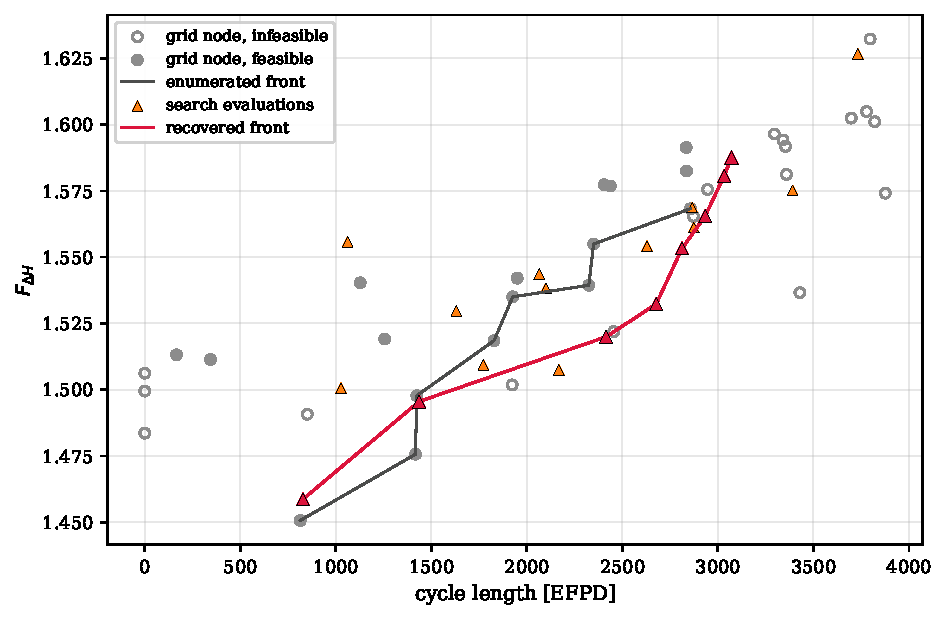
\includegraphics[width=0.92\linewidth]{images/valgrid_objective}
  \caption[Enumerated and recovered fronts in the objective
  plane]{Objective plane of the two-variable slice, with the 35
  enumerated grid nodes, the 20 search evaluations and the two feasible
  non-dominated sets.}
  \label{fig:valgrid-objective}
\end{figure}

Four readings follow from the table and from
Figure~\ref{fig:valgrid-objective}.

\begin{enumerate}
  \item The search recovered a front of the same size at a lower cost.
        Both fronts hold eight members. The search used 20 truth
        evaluations against 35, that is \SI{57}{\%} of the count, and
        \SI{4.9}{h} of wall clock against \SI{8.5}{h}, that is
        \SI{58}{\%} of the time.

  \item The recovered front has the larger hypervolume, 209.7 against
        193.1, a ratio of 1.086. Section~\ref{sec:validation-grid}
        anticipates a ratio above one, because the search places designs
        anywhere in the box while the enumeration is confined to grid
        nodes.

  \item The recovered front dominates most of the enumerated front. The
        union of the two fronts retains all eight recovered members and
        only three of the eight enumerated members, so five enumerated
        members are dominated outright. The strict coverage of 0.62
        rises to 0.75 when a tolerance of 0.02 in the normalised
        objectives is allowed.

  \item The domination is not complete. The additive epsilon indicator
        is 0.145 in the normalised space, equivalent to \SI{328}{EFPD}
        on the cycle length or to 0.0199 on the peaking factor. The
        binding point is on the short-cycle portion of the enumerated
        front, near \SI{1420}{EFPD}, where the recovered front sits
        about 0.02 higher in $F_{\Delta H}$.
\end{enumerate}

The acquisition also spent its evaluations better. Of the 35 enumerated
nodes 17 are feasible, \SI{48.6}{\%}, against 15 of the 20 search
evaluations, \SI{75.0}{\%}. Figure~\ref{fig:valgrid-design} shows the
same comparison in the design plane.

\begin{figure}[htbp]
  \centering
  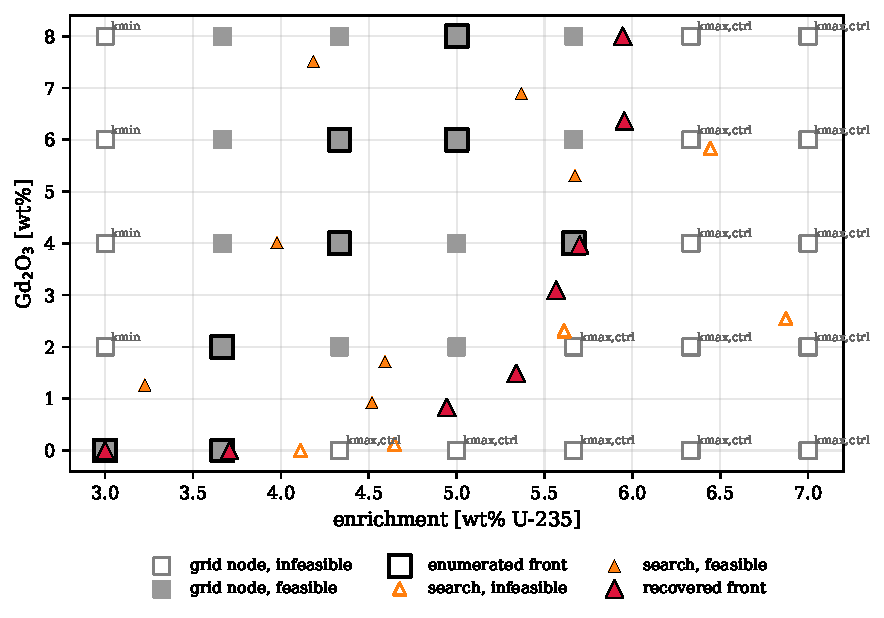
\includegraphics[width=0.92\linewidth]{images/valgrid_design}
  \caption[The two fronts in the design plane of the slice]{Design plane
  of the two-variable slice. Infeasible grid nodes are annotated with
  the constraint they violate.}
  \label{fig:valgrid-design}
\end{figure}

Figure~\ref{fig:valgrid-design} shows where the two fronts sit in the
design plane, and it answers where the difference of \SI{8.6}{\%} in
hypervolume comes from.

The feasible band of the slice is bounded on both sides by a reactivity
constraint. The nodes at \SI{3.0}{wt\%} enrichment with gadolinia at or
above \SI{2}{wt\%} fail the lower reactivity bound $k_\mathrm{min}$. The
nodes at \SI{6.33}{wt\%} and above, together with the unpoisoned nodes
from \SI{4.33}{wt\%} upward, fail the controllability screen. No node in
the slice fails on peaking.

The enumerated front is confined to the five gadolinia values of the
grid, 0, 2, 4, 6 and \SI{8}{wt\%}. The recovered front places three of
its eight members between 0 and \SI{2}{wt\%}, at 0.8, 1.45 and
\SI{3.05}{wt\%} with enrichments of 4.95, 5.35 and \SI{5.57}{wt\%},
inside a band that the grid does not sample. It also reaches
\SI{5.95}{wt\%} enrichment, beyond the last feasible grid column at
\SI{5.67}{wt\%}, and therefore extends the front to \SI{3070}{EFPD}
against \SI{2840}{EFPD} for the enumeration.

Figure~\ref{fig:valgrid-surrogate} tests the surrogate on the grid nodes
it has not seen.

\begin{figure}[htbp]
  \centering
  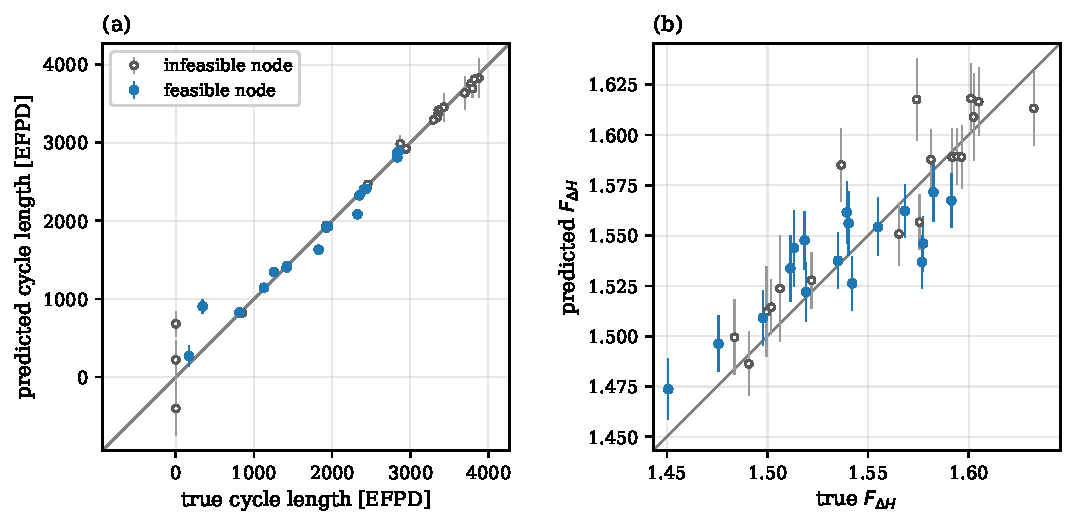
\includegraphics[width=\linewidth]{images/valgrid_surrogate}
  \caption[Surrogate prediction at the unseen grid nodes]{Surrogate prediction at the 35 unseen grid nodes. Error bars are one predictive standard deviation.}
  \label{fig:valgrid-surrogate}
\end{figure}

The last check of Section~\ref{sec:validation-grid} is a pure
extrapolation test. The surrogate fitted on the 20 search evaluations is
evaluated at all 35 grid nodes, none of which entered its training set.
Figure~\ref{fig:valgrid-surrogate} gives the result. The cycle length
follows the diagonal over the whole range, with the same departure at
the short-cycle end already seen in Figure~\ref{fig:c8-cv-loo}. The
peaking factor scatters more widely, and the one-sigma bars of most
nodes intersect the diagonal.

Two limits bound this exercise. The slice is two-dimensional, so it
tests the search on a problem an order of magnitude smaller than the
four-variable campaign, and the enumeration grid is coarse in gadolinia,
which is the very axis on which the recovered front gains its
hypervolume.

%% AUTHOR: two or three sentences of physics on why the low-gadolinia,
%% high-enrichment corridor of Figure~\ref{fig:valgrid-design} is the
%% one that carries the front, and on whether the same corridor is
%% visible in the full four-variable archive of
%% Section~\ref{sec:res-c8-front}.

%% AUTHOR: one sentence on whether an 8.6 per cent hypervolume gain at
%% 57 per cent of the evaluations is the claim you want to make for the
%% framework, or whether the epsilon indicator of 328 EFPD is the more
%% conservative headline.


\subsection{The two-bank subset}
\label{sec:res-c8-split}

Table~\ref{tab:c8-two} lists the four feasible designs that the first
two banks alone hold subcritical at the margin. Design 12 is included
for completeness and is not a candidate. The four designs occupy the
narrow reactivity window of Equation~\eqref{eq:two-bank-ceiling}, with
unrodded eigenvalues between 1.026 and 1.042, and none of them is on
the front, because the front is defined by cycle length and they carry
a beginning-of-life excess of only \num{2564} to \SI{4068}{pcm}.

\begin{table}[htbp]
  \centering
  \small
  \caption[The Campaign 8 two-bank subset]{Feasible Campaign 8 designs controllable with the first two banks. Columns as in Table~\ref{tab:c8-front}.}
  \label{tab:c8-two}
  \setlength{\tabcolsep}{3.8pt}
  \begin{tabular}{cccccccccc}
    \toprule
    Design & EFPD & rings & $w_\mathrm{Gd}$ & $n_\mathrm{Gd}$ &
      $t_\mathrm{refl}$ & $k^\mathrm{core}$ & excess & $F$ & $F_{2}$ \\
    {[--]} & [d] & [wt\%] & [wt\%] & [rods] & [cm] & [--] & [pcm] &
      [--] & [--] \\
    \midrule
    53 & 1142 & 2.48, 3.08, 3.97 & 2.92 & 12 & 4.74 & 1.026 & 2564 & 1.524 & 2.020 \\
    13 & 2383 & 3.70, 4.59, 5.91 & 5.25 & 24 & 3.15 & 1.042 & 4068 & 1.632 & 2.131 \\
    31 & 3381 & 4.74, 5.89, 7.58 & 3.38 & 40 & 4.18 & 1.034 & 3282 & 1.650 & 2.074 \\
    12 &  598 & 3.47, 4.30, 5.54 & 7.06 & 20 & 2.46 & 1.033 & 3207 & 1.592 & 2.061 \\
    \bottomrule
  \end{tabular}
\end{table}

The subset is where the operating physics of a pressurised water
reactor is recognisable. A commercial core at hot full power holds its
beginning-of-life excess with soluble boron and burnable absorber and
keeps the regulating banks nearly withdrawn, so that the rods carry
only the power defect and the manoeuvring band. The eight front
designs would need the four regulating banks inserted deep enough to
hold \num{8930} to \SI{13627}{pcm} at power with \SI{1000}{ppm} in the
coolant, which no pressurised water reactor does, and which would
impose the rodded peaking of Figure~\ref{fig:c8-split} continuously.
The two-bank designs hold \num{2564} to \SI{4068}{pcm}, of the order
that boron adjustment alone can carry.

The comparison with a licensed-class core makes the point
quantitative. The NuScale-like benchmark on which the fuel design of
this thesis rests reports, at beginning of life with \SI{1000}{ppm} of
soluble boron, a fuel temperature of \SI{900}{K} and a coolant
temperature of \SI{600}{K}, a reference all-rods-out eigenvalue of
$1.02768 \pm 0.00001$~\cite{fridman_nuscale_benchmark_2023}, which an
OpenMC model with ENDF/B-VII.1 reproduces within 16 to
\SI{31}{pcm}~\cite{ez_aldeen_2025}.
Its sixteen control rod assemblies, in four banks of four, are worth
\num{1965}, \num{2379}, \num{3727} and \SI{3728}{pcm} individually and
\SI{19231}{pcm} all together. The regulating requirement of that core
at beginning of life is therefore below \SI{2800}{pcm}, held by one
bank with margin, and the shutdown banks are reserved.
Table~\ref{tab:bench-compare} places the two Campaign 8 candidate
lists against it. The worth column is for sixteen control rod
assemblies in every case, namely the four banks of the benchmark
together and the four regulating banks of this core.

\begin{table}[htbp]
  \centering
  \small
  \caption[Reactivity to be held by the rods, against the
  benchmark]{Beginning-of-life reactivity to be held by the rods at \SI{1000}{ppm}: NuScale-like benchmark and the two Campaign 8 candidate lists.}
  \label{tab:bench-compare}
  \begin{tabularx}{\textwidth}{@{}>{\raggedright\arraybackslash}X ccc@{}}
    \toprule
    Core & $k_\mathrm{eff}^\mathrm{core}$ & excess to hold &
      worth of 16 CRA \\
     & [--] & [pcm] & [pcm] \\
    \midrule
    NuScale-like benchmark~\cite{fridman_nuscale_benchmark_2023}
      & 1.028 & 2700 & 19231 \\
    Campaign 8 front, Table~\ref{tab:c8-front}
      & 1.098 to 1.158 & 8930 to 13627 & 14270 to 17665 \\
    Campaign 8 two-bank subset, Table~\ref{tab:c8-two}
      & 1.026 to 1.042 & 2564 to 4068 & 13906 to 16303 \\
    \bottomrule
  \end{tabularx}
\end{table}

The rods are alike. Sixteen assemblies of this core are worth
\num{11466} to \SI{19313}{pcm} across the archive, the same range as
the sixteen of the benchmark, because the rod design, the absorber
densities and the guide-tube geometry are the benchmark's. What
differs is how much the rods are asked to hold. The two-bank subset
sits in the regime of the benchmark. The front asks three to five
times what a licensed-class small core asks of its rods at start-up,
and it can only be held with the four regulating banks inserted deep
at power.


The two requirements pull in opposite directions because a longer
cycle is bought with reactivity that is burned later, and that
reactivity must be held at the start of life. With the soluble boron
and the gadolinia already present in every eigenvalue of this work,
whatever the burnup has not yet consumed is held by the rods, so the
excess that lengthens the cycle is the same excess that drives the
regulating banks into the core. The consequence for the formulation is
drawn in Section~\ref{sec:concl-reform}: the cycle length becomes a
constraint at the required value and the two-bank eigenvalue an
objective. That is a stronger use of the two-bank reading than a
constraint would be, since a constraint would only bound the margin
whereas an objective maximises it.


\subsection{Burnup and composition dependence of the leakage
correction}
\label{sec:res-kt-burnup}

The leakage-corrected target of Equation~\eqref{eq:ktarget} rests on
two assumptions that the closure check of
Section~\ref{sec:res-corevalidation} does not reach. The leakage
factor is evaluated once, at beginning of life, on a single reference
composition of \num{4.55} and \SI{4.05}{\percent} by weight without
gadolinia, and it is then held constant over the whole cycle and
applied to every design in the space. Both assumptions are tested
here, on the eight front designs of Table~\ref{tab:c8-front} and on
the two-bank representatives of Table~\ref{tab:c8-two}.

For each design the reflective assembly is depleted once, in a single
shot with the campaign schedule, up to two steps beyond its end of
cycle. At beginning of life and at the two depletion steps that
bracket the end of cycle, the depleted composition is loaded uniformly
into all \num{32} assemblies of the core model of
Section~\ref{sec:meth-ktarget} and into the reflective assembly, and
both eigenvalues are solved with three independent seeds. The measured
leakage factor follows.

\begin{equation}
\mathrm{LF}(B) =
\frac{k_\infty^\mathrm{assembly}(B)}{k_\mathrm{eff}^\mathrm{core}(B)}
\; L_\mathrm{ax}
\label{eq:kt-lf}
\end{equation}

\noindent where the symbols have the following meaning.

\begin{itemize}
  \item $\mathrm{LF}(B)$ is the leakage factor measured at burnup $B$
        on the design's own depleted composition, dimensionless.

  \item $k_\infty^\mathrm{assembly}(B)$ is the infinite multiplication
        factor of the reflective assembly at burnup $B$,
        dimensionless.

  \item $k_\mathrm{eff}^\mathrm{core}(B)$ is the effective
        multiplication factor of the \num{32}-assembly core built with
        the same reflector thickness, loaded uniformly with the same
        depleted composition and closed by a vacuum radial boundary,
        dimensionless.

  \item $L_\mathrm{ax}$ is the axial leakage factor of
        Section~\ref{sec:meth-lax}, equal to \num{1.0289},
        dimensionless.

  \item $B$ is the burnup, in MWd/kgHM.
\end{itemize}

Two quantities are read from the measurement. The drift is the change
of the leakage factor between the two ends of the cycle and tests the
burnup assumption. The residual is the leakage factor minus the
tabulated target and tests the composition assumption. The residual at
the end of cycle is the one that moves the reported cycle length,
through the local reactivity slope of the assembly.

\begin{equation}
\Delta\mathrm{EFPD} =
\frac{\mathrm{LF}(B_\mathrm{EOC}) - k_\mathrm{target}}
     {\left. \mathrm{d}k_\infty / \mathrm{d}B \right|_{B_\mathrm{EOC}}}
\; \frac{1000}{q}
\label{eq:kt-defpd}
\end{equation}

\noindent where the symbols have the following meaning.

\begin{itemize}
  \item $\Delta\mathrm{EFPD}$ is the correction to the reported cycle
        length, in effective full-power days.

  \item $\mathrm{LF}(B_\mathrm{EOC})$ is the leakage factor of
        Equation~\eqref{eq:kt-lf} at the end-of-cycle burnup,
        dimensionless.

  \item $k_\mathrm{target}$ is the tabulated target the optimiser used
        for that design, dimensionless.

  \item $\mathrm{d}k_\infty / \mathrm{d}B$ is the local reactivity
        slope of the assembly between the two bracketing depletion
        steps, in (MWd/kgHM)$^{-1}$, negative at the end of cycle.

  \item $q$ is the core specific power, equal to
        \SI{9.9834}{\watt\per\gram} of heavy metal
        (Table~\ref{tab:model-operating}).

  \item $B_\mathrm{EOC}$ is the end-of-cycle burnup, in MWd/kgHM.
\end{itemize}

Table~\ref{tab:kt-burnup} reports the measurement. Every design ended
its cycle on the reactivity crossing, so no entry is set by the burnup
cap.

\begin{table}[htbp]
  \centering
  \small
  \caption[Burnup dependence of the Route B leakage factor]{Burnup
  dependence of the Route B leakage factor on the Campaign 8 designs.}
  \label{tab:kt-burnup}
  \setlength{\tabcolsep}{4.2pt}
  \begin{tabular}{ccccccccc}
    \toprule
    Design & $e$ & $t_\mathrm{refl}$ & $B_\mathrm{EOC}$ &
      $k_\mathrm{target}$ & $\mathrm{LF}_\mathrm{BOL}$ &
      $r_\mathrm{BOL}$ & drift & $\Delta\mathrm{EFPD}$ \\
    {[--]} & [wt\%] & [cm] & [MWd/kgHM] & [--] & [--] & [pcm] & [pcm] &
      [d] \\
    \midrule
     1 & 11.03 & 3.94 & 57.8 & 1.0829 & 1.0793 & $-329$ & $+33 \pm 126$ & $+56$ \\
    59 &  9.34 & 5.66 & 50.2 & 1.0820 & 1.0796 & $-220$ & $ -4 \pm 107$ & $+43$ \\
    44 &  9.23 & 5.33 & 49.8 & 1.0822 & 1.0798 & $-219$ & $-10 \pm  90$ & $+42$ \\
    21 &  7.81 & 4.92 & 42.3 & 1.0824 & 1.0800 & $-222$ & $+149 \pm 84$ & $+11$ \\
    31 &  6.59 & 4.18 & 33.4 & 1.0828 & 1.0819 & $ -85$ & $-10 \pm  85$ & $+14$ \\
    29 &  5.90 & 4.69 & 31.0 & 1.0825 & 1.0824 & $  -9$ & $-152 \pm 99$ & $+25$ \\
    23 &  4.94 & 4.81 & 23.7 & 1.0824 & 1.0830 & $ +53$ & $-67 \pm 116$ & $ +2$ \\
    42 &  4.44 & 3.76 & 19.7 & 1.0830 & 1.0836 & $ +54$ & $-22 \pm  82$ & $ -4$ \\
    47 &  4.39 & 4.29 & 19.5 & 1.0827 & 1.0830 & $ +27$ & $ +2 \pm 107$ & $ -4$ \\
    53 &  3.45 & 4.74 & 10.8 & 1.0825 & 1.0844 & $+174$ & $-84 \pm  88$ & $-14$ \\
    \bottomrule
  \end{tabular}
\end{table}

The burnup assumption holds. No single drift is resolved at two
standard deviations, the largest ratio of value to uncertainty being
\num{1.78} on design 21. The ten drifts are ten independent
measurements of the same physical quantity, so they are combined by
inverse-variance weighting.

\begin{equation}
\overline{\Delta\mathrm{LF}} = -13 \pm \SI{30}{pcm},
\qquad
\chi^2 = 6.73 \ \text{on 9 degrees of freedom}
\label{eq:kt-comp}
\end{equation}

The weighted mean is \num{0.43} standard deviations from zero. The
reduced chi-squared of \num{0.75}, with a probability of \num{0.66},
states that the observed scatter of the ten values is accounted for by
the Monte Carlo uncertainties alone, so the data support neither a
common drift nor a design-dependent one. The bound to quote is
\SI{60}{pcm} at two standard deviations on the mean, which corresponds
to \num{7} to \SI{11}{d} at the local reactivity slopes of the table,
below \SI{0.9}{\percent} of every reported cycle. The frozen leakage
factor is therefore justified over the cycle.

The composition assumption does not hold, and this is the substantive
result. The beginning-of-life residual runs from $+174$ to
\SI{-329}{pcm} and is almost perfectly ordered by enrichment.

\begin{itemize}
  \item The Pearson correlation between $r_\mathrm{BOL}$ and the
        enrichment is $-0.975$, against $-0.234$ for the reflector
        thickness, so the effect is compositional and not geometric.

  \item The linear fit is $r_\mathrm{BOL} = 341 - 62.5\,e$ in pcm,
        with $e$ the enrichment in per cent by weight, a slope
        uncertainty of $\pm 5.0$\,pcm per weight per cent and a
        root-mean-square residual of \SI{38}{pcm}, which is inside the
        statistics of a single solve.

  \item The residual passes through zero near \SI{5.5}{\percent} by
        weight, close to the reference composition on which the table
        was built, and grows to \SI{-329}{pcm} at the
        \SI{11.03}{\percent} of design 1.
\end{itemize}

An independent sweep of 48 core solves checks both slopes of the
target. It gives an enrichment slope of $-64.1 \pm 3.2$\,pcm per weight
per cent, 0.3 combined standard deviations from the validation value.
It gives a reflector slope of $-25.1 \pm 4.0$\,pcm per centimetre,
against the $-47.6 \pm 15.7$\,pcm per centimetre of the target table
once the uncertainty of its slope is recovered, a separation of 1.39
standard deviations, and a second determination at the reference
composition lies 1.47 standard deviations away. The three
determinations are consistent (Section~\ref{sec:meth-limits-sigma}).
The same sweep resolves a quadratic term in enrichment, which makes a
single enrichment slope a secant (Section~\ref{sec:meth-limits-secant}).

The sign is the one a two-group argument predicts. The non-leakage
probability of a bare core is governed by the product of the geometric
buckling and the migration area, and raising the enrichment raises the
absorption cross section, shrinks the migration area, and reduces the
relative leakage. A more reactive core therefore needs a smaller
leakage correction than the reference composition of the table
supplies.

The consequence for the reported results is bounded and directional. A
negative residual means the frozen table demanded more reactivity than
the depleted core required, so Route B was conservative and the
reported cycle length is a lower bound. This is the case for the six
longest-cycle designs, with corrections of $+11$ to \SI{+56}{d}, that
is \num{0.3} to \SI{1.0}{\percent}. The sign reverses below the
reference composition, and design 53 is overstated by \SI{14}{d}, or
\SI{1.3}{\percent}. Applying the correction of
Equation~\eqref{eq:kt-defpd} to all ten designs leaves the ordering of
Table~\ref{tab:c8-front} unchanged, including the \SI{27}{d} gap
between designs 42 and 47, because the objective differences on the
front are of the order of hundreds of days.

The measurement also delivers an independent replicate of the cycle
length itself. The depletion here was run in a single shot, while the
campaign ran it in chunks of two steps, and the two used different
random-number seeds, because the seed is a hash of the design
dictionary and the two dictionaries carry different key sets. Across
the nine designs whose end of cycle falls on a \SI{4}{MWd\per\kilo
\gram} step, the cycle lengths agree to a mean of
\SI{+0.09}{\percent} with a standard deviation of
\SI{0.91}{\percent}. This is the first direct measurement of the
Monte Carlo uncertainty on cycle length in this work, and it also
confirms that the chunked restart of the campaign carries no
systematic bias.

Three limits of the measurement should be stated.

\begin{enumerate}
  \item The depleted composition is loaded uniformly into all
        \num{32} assemblies. This reproduces the construction of the
        calibration table exactly, which is what the check requires,
        but it does not represent the radial burnup distribution of an
        operating core, in which the periphery burns more slowly than
        the centre.

  \item The end-of-cycle leakage factor is interpolated linearly
        between the two bracketing depletion steps, which are up to
        \SI{4}{MWd\per\kilo\gram} apart. The interpolation error is
        second order in that interval and is not separated from the
        statistical uncertainty.

  \item Design 53 ends its cycle at \SI{10.8}{MWd\per\kilo\gram},
        inside the beginning-of-life block, so its crossing is
        interpolated across the \SI{6}{MWd\per\kilo\gram} interval
        between the depletion points at \num{7.5} and
        \SI{13.5}{MWd\per\kilo\gram}. Its cycle length is
        correspondingly more sensitive to eigenvalue noise, and it is
        the one design whose two replicates differ by more than
        \SI{1.5}{\percent}, at \SI{-4.8}{\percent}. The coarse
        beginning-of-life block is adequate for the long-cycle
        designs and marginal for the short-cycle ones.
\end{enumerate}

The composition dependence is reported here as a limitation of
Route~B. A refit of the target table as a function of enrichment as
well as reflector thickness would close it in follow-on work, and the
measured slope of $-62.5 \pm 5.0$\,pcm per weight per cent is the coefficient
such a refit would need.

\subsection{Reactivity swing, the hump and the critical boron}
\label{sec:res-c8-swing}

The single-shot depletions of Section~\ref{sec:res-kt-burnup} carry the
full $k_\infty(B)$ history of each candidate, so the hump of
Equation~\eqref{eq:c7-hump} and the burnup reactivity swing can be
measured on Campaign 8 with no further transport.
Figure~\ref{fig:c8-swing-khist} shows the histories of the eight front
designs and of designs 53 and 31, with their maxima marked by triangles
and the leakage-corrected target dotted. Table~\ref{tab:c8-swing}
reports the quantities for all eleven candidates, including design 13,
whose history is not drawn in the figure.

\begin{figure}[htbp]
  \centering
  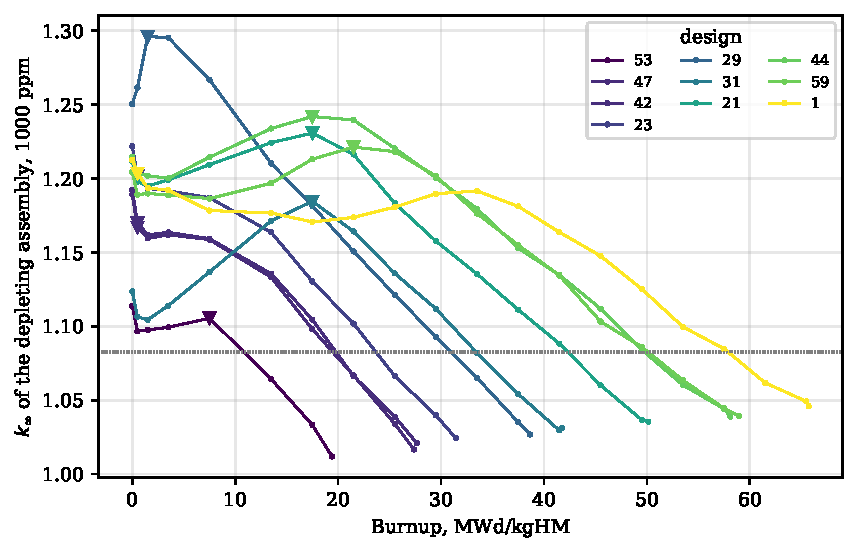
\includegraphics[width=0.95\linewidth]{images/swing_khist}
  \caption[Depletion histories of the Campaign 8 candidates]{Assembly infinite multiplication factor against burnup at \SI{1000}{ppm} for the eight front designs and the two two-bank representatives.}
  \label{fig:c8-swing-khist}
\end{figure}

\begin{table}[htbp]
  \centering
  \footnotesize
  \setlength{\tabcolsep}{3.0pt}
  \begin{threeparttable}
  \caption[Reactivity swing of the Campaign 8 candidates]{Gadolinium hump and burnup reactivity swing of the Campaign 8 candidates.}
  \label{tab:c8-swing}
  \begin{tabular}{@{}r r r r r r r r r r@{}}
    \toprule
    ID & $e$ & $k_\mathrm{BOL}$ & $k_\mathrm{peak}$ & $B_\mathrm{peak}$ & hump & $\Delta\rho_\mathrm{peak\to EOC}$ & $\Delta\rho_\mathrm{Xe\to EOC}$ & $c_\mathrm{BOL}$ & $c_\mathrm{peak}$ \\
    {[--]} & [wt\%] & [--] & [--] & [MWd/kgHM] & [pcm] & [pcm] & [pcm] & [ppm] & [ppm] \\
    \midrule
    53 & 3.45 & 1.1138 & 1.1055 & 7.5 & -676 & 1922 & 1196 & 1312 & 1312 \\
    47 & 4.39 & 1.1891 & 1.1670 & 0.5 & -1591 & 6673 & 6673 & 2348 & 2348 \\
    42 & 4.44 & 1.1922 & 1.1701 & 0.5 & -1578 & 6875 & 6875 & 2377 & 2377 \\
    23 & 4.94 & 1.2219 & 1.2019 & 0.5 & -1356 & 9184 & 9184 & 2979 & 2979 \\
    13 & 5.14 & 1.1302 & 1.1210 & -- & -723 & 3103 & 2106 & 1697 & 1697 \\
    29 & 5.90 & 1.2504 & 1.2961 & 1.5 & +2822 & 15225 & 13102 & 3677 & 4277 \\
    31 & 6.59 & 1.1236 & 1.1846 & 17.5 & +4580 & 7936 & 1971 & 1701 & 2760 \\
    21 & 7.81 & 1.2114 & 1.2307 & 17.5 & +1295 & 11136 & 8914 & 3752 & 4095 \\
    44 & 9.23 & 1.2147 & 1.2420 & 17.5 & +1812 & 11892 & 9340 & 4372 & 4940 \\
    59 & 9.34 & 1.2043 & 1.2212 & 21.5 & +1150 & 10538 & 8319 & 4112 & 4473 \\
    1 & 11.03 & 1.2127 & 1.2036 & 0.5 & -626 & 9257 & 9257 & 4674 & 4674 \\
    \bottomrule
  \end{tabular}
  \begin{tablenotes}\footnotesize
    \item Assembly $k_\infty$ at 1000\,ppm from the single-shot depletion of \nolinkurl{validate_ktarget_burnup.py} at the campaign fidelity. The hump is $\rho_\mathrm{peak} - \rho_\mathrm{BOL}$, xenon-free BOL. $\Delta\rho$ is measured to $\rho(k_\mathrm{target})$. The boron concentrations are linear extrapolations above 1000\,ppm with the 1000 to 1500\,ppm differential worth of the core. They are estimates: for design 47 the root of the measured reactivity curve is 2327\,ppm (Section~\ref{sec:res-c8-mtc}). $B_\mathrm{peak}$ was not recorded for design 13.
  \end{tablenotes}
  \end{threeparttable}
\end{table}

Four readings follow.

\begin{enumerate}
  \item Six of the eleven candidates have no hump. Designs 1, 13, 23,
        42, 47 and 53 reach their maximum at the first operating point,
        and their hump is negative, from $-626$ to \SI{-1591}{pcm}. For
        these designs the beginning-of-life state is the most reactive
        state of the cycle and the screens of
        Section~\ref{sec:meth-ctrl} screen the right state.

  \item The other five do have one, from $+1150$ to \SI{+4580}{pcm},
        with the maximum between \num{1.5} and
        \SI{21.5}{MWd/kgHM}. Design 31 carries the largest hump of the
        set and design 29 the largest of the front, at
        \SI{+2822}{pcm}.

  \item The hump is not ordered by the gadolinia loading of
        Table~\ref{tab:c8-front}. Design 1 carries \SI{7.43}{wt\%}
        gadolinia on forty pins and shows no hump, while design 29
        carries \SI{0.18}{wt\%} on forty pins and shows the largest
        hump of the front.

  \item The campaign was screened at a boron concentration well below
        the critical one. The extrapolated critical concentration at
        beginning of life runs from \num{1312} to \SI{4674}{ppm}, and
        at the operating maximum it reaches \SI{4940}{ppm} on design
        44. The values are linear extrapolations above \SI{1500}{ppm}
        and can err in either direction. For design 47 the root of the
        measured reactivity curve, \SI{2327}{ppm}, lies \SI{21}{ppm}
        below the linear value (Section~\ref{sec:res-c8-mtc}).
\end{enumerate}

The last reading is the one that bounds the interpretation of the whole
campaign. The screens were evaluated at the fixed \SI{1000}{ppm} of
Section~\ref{sec:meth-boron}, which is not the concentration at which
any of these cores would be critical at start-up. The direction of the
resulting bias is the one stated in
Section~\ref{sec:meth-boron-bias}, and the magnitudes here give it a
scale for the first time.

Two approximations bound the boron columns. The swing is an assembly
quantity while the differential boron worth is a core quantity measured
at beginning of life, so dividing one by the other assumes the worth
does not change over the cycle, which it does through the spectrum.
Both concentrations should be read to one significant figure.

%% AUTHOR: the physics of why six candidates show no hump while five
%% do, and whether the critical-boron column changes the reading of the
%% controllability result of Section~\ref{sec:res-c8-split}.

\subsection{Three-dimensional confirmation: the four closures}
\label{sec:res-c8-closures}

Four commitments were made earlier in this work and deferred to a
confirmation on the three-dimensional core model. This
subsection reports what each of them measured. Two are closed, one is
partly closed and one remains open.

The three-dimensional confirmation closes four commitments made earlier
in this work. Each is listed with the quantity that closes it, and
Table~\ref{tab:c8-closures} collects the measured closures.

\begin{enumerate}
  \item The second tier of the fidelity strategy of Section~\ref{sec:meth-fidelity}. Ten front designs were depleted in a single shot at the campaign fidelity with core solves at beginning and end of cycle. The leakage factor drifts by -152 to +149\,pcm between the two, within two standard deviations for 10 of 10 designs, and the implied cycle correction is -14 to +56\,EFPD.
  \item The axial correction of Section~\ref{sec:meth-lax}. On the three-dimensional core model the unrodded factor is 1.0286 to 1.0311, against the campaign value 1.0289 of the water-slab study, a gap of -25 to +211\,pcm. The two-bank factor is 1.0219 to 1.0252 and the four-bank factor 1.0126 to 1.0177.
  \item The three departures from the benchmark inputs stated in Section~\ref{sec:reactor-model}, tested on C8-21 and C8-47, which bracket the front. Raising the steel fraction of the heavy reflector from 0.90 to the benchmark 0.956 adds 199 and 182\,pcm to the unrodded three-dimensional core, so the adopted fraction is conservative. Narrowing the absorber radius from 0.4331\,cm to the benchmark boron carbide radius of 0.4229\,cm lowers the four-bank worth by 131 to 169\,pcm and the two-bank worth by 93 to 94\,pcm, about 1.5 per cent of the two-bank worth, against margins of 7000\,pcm and more. The coolant density is not exposed as a sensitivity and remains a stated departure.
  \item The rod-stack comparison. The two-dimensional screen with full-height boron carbide is conservative by 1272 to 2047\,pcm for four banks and 2062 to 2671\,pcm for two banks against the benchmark rod on the three-dimensional core. \openpoint{Closure 4: the full-B4C stack run that separates the stack from the leakage is pending.}
\end{enumerate}

\begin{table}[htbp]
  \centering
  \footnotesize
  \setlength{\tabcolsep}{4.0pt}
  \caption[Closures of the three-dimensional confirmation]{Measured closure of the four commitments carried by the three-dimensional confirmation.}
  \label{tab:c8-closures}
  \begin{tabularx}{\textwidth}{@{}>{\raggedright\arraybackslash}p{2.6cm} >{\raggedright\arraybackslash}X r >{\raggedright\arraybackslash}X r@{}}
    \toprule
    Closure & Quantity & Value & Quantity & Value \\
    \midrule
    1 Second tier & leakage-factor drift BOL to EOC [pcm] & -152 to +149 & implied cycle correction [EFPD] & -14 to +56 \\
    2 Axial correction & $L_\mathrm{ax,hw}$ unrodded & 1.0286 to 1.0311 & gap to the campaign 1.0289 [pcm] & -25 to +211 \\
    3a Reflector 0.956 & $\Delta\rho$ unrodded 3D [pcm] & +182 to +199 &  &  \\
    3b Absorber 0.4229 & $\Delta$ four-bank margin [pcm] & -169 to -131 & $\Delta$ two-bank margin [pcm] & -94 to -93 \\
    4 Rod stack & screen conservatism four-bank [pcm] & 1272 to 2047 & stack effect four-bank [pcm] & pending \\
    \bottomrule
  \end{tabularx}
\end{table}

Closure 1 is not an independent measurement. It is the same set of
solves reported in Section~\ref{sec:res-kt-burnup}, read there for the
burnup dependence of the leakage factor and read here as the second
fidelity tier. The drift range and the cycle correction of
Table~\ref{tab:c8-closures} are the drift and $\Delta\mathrm{EFPD}$
columns of Table~\ref{tab:kt-burnup}, and they are quoted once as
evidence for two different commitments.

Closures 2 and 4 are read in full in
Section~\ref{sec:res-c8-3d}, where the rodded axial factors, the
benchmark rod stack and the resulting conservatism of the
two-dimensional screen are measured design by design against
Table~\ref{tab:c8-post-3d1000}. The short statement is that the rodded
factors are smaller than the unrodded one, so the rodded
three-dimensional core is more subcritical than the two-dimensional
screen assumed, and the screen therefore rejected designs it did not
need to reject while admitting none that the three-dimensional core model would refuse.

The beginning-of-life margins above are reduced by the gadolinium hump of the operating maximum, -1723 to +4955\,pcm on the core. At the maximum the two-bank set at 1000\,ppm on the three-dimensional core excludes designs 1, 21, 23, 29, 31, 44, 59.

The hump range quoted here is the assembly hump of
Table~\ref{tab:c8-swing} carried to the core, which is larger than the
assembly value by the leakage factor, and it is applied to the
beginning-of-life margins because
Section~\ref{sec:res-kt-burnup} shows the leakage factor constant over
the cycle within the Monte Carlo noise.

%% AUTHOR: physics of the hump and its consequence for the candidate.

%% AUTHOR: whether the exclusion of seven of the ten candidates from
%% the two-bank set at the operating maximum is the argument that
%% decides the candidate list of Section~\ref{sec:res-c8-limits}, and
%% what the remaining designs have in common.

\subsection{Cycle length against the reported refuelling interval}
\label{sec:res-c8-mission}

The open record gives the prototype a refuelling interval of five
years~\cite{dinizcosta_2017}. The cycle
length that corresponds to it depends on the capacity factor, which
no open source states.

\begin{equation}
\mathrm{EFPD}_\mathrm{req} = 365.25\, T_\mathrm{cal}\, \mathrm{CF}
\label{eq:mission-efpd}
\end{equation}

\noindent where the symbols have the following meaning.

\begin{itemize}
  \item $\mathrm{EFPD}_\mathrm{req}$ is the cycle length that meets the
        refuelling interval, in effective full power days.

  \item $T_\mathrm{cal}$ is the calendar interval, in years, equal to
        five.

  \item $\mathrm{CF}$ is the capacity factor, dimensionless, assumed
        between 0.5 and 0.8 for a naval prototype and stated as an
        assumption.
\end{itemize}

Five years at a capacity factor of 0.8 is 1461 EFPD, and at 0.5 it is
913 EFPD. Every design on the front exceeds the former, the shortest by
a third and the longest by a factor of four, and design 53 in the
two-bank subset meets it at 1142 EFPD with ring enrichments of 2.5,
3.1 and \SI{4.0}{wt\%}. The reported enrichment figures locate on the
same axis. The 6 to \SI{8}{wt\%} stated in 2014 corresponds to designs
31 and 21, at 3381 and 4221 EFPD, and the \SI{19}{wt\%} reported in
2025 lies above the search box and, on the evidence of the axial study,
above what the regulating banks of this core can hold. The comparison
is conservative on two counts. Every cycle length is a lower bound
for a core operated with boron letdown
(Section~\ref{sec:res-c8-post-limits}), and the burnup dependence of
the leakage factor corrects the six longest cycles downward
(Section~\ref{sec:res-kt-burnup}).

The consequence for the design problem is stated as a finding. The
objective of maximising cycle length pushes every design far beyond
the reported requirement and, in doing so, onto the control boundary.
Cycle length is not the binding requirement of this core. The binding
requirements are controllability and peaking, and the cycle length
belongs among the constraints, at the required value. Campaign 9 poses
the problem that way (Section~\ref{sec:res-c9}).

\subsection{The pre-registered expectations, scored}
\label{sec:res-c8-hyp}

Table~\ref{tab:c8-hyp-scored} scores the eight expectations written before
the design of experiments closed against the measurement.

\begin{table}[htbp]
  \centering
  \small
  \caption{The eight expectations written before the design of
  experiments closed, against the measurement.}
  \label{tab:c8-hyp-scored}
  \begin{tabularx}{\textwidth}{@{}>{\raggedright\arraybackslash}X>{\raggedright\arraybackslash}p{1.6cm}>{\raggedright\arraybackslash}X@{}}
    \toprule
    Expectation & Outcome & Measurement \\
    \midrule
    Peaking floor rises to about 1.60 & Failed & Floor 1.510, reached through low enrichment rather than a thick reflector \\
    Cycles 450 to 500 EFPD shorter than uncorrected & Not testable & No uncorrected Campaign 8 run exists, and the box differs from Campaign 7 \\
    Two banks worth half of sixteen & Held & Ratio 0.473 to 0.511, mean 0.496, on all 60 designs \\
    Two-bank window below about 1.074 & Held & Feasible two-bank designs at 1.026 to 1.042, median implied ceiling 1.069 \\
    Ceiling binds rarely and after the screen & Held & Zero designs rejected by the ceiling alone \\
    Every block moves all four variables & Partly held & Block 1 held $w_\mathrm{Gd}$ fixed, every block moved three or more and returned feasible designs \\
    Design-of-experiments feasibility below \SI{31}{\%} & Held & 9 of 36, \SI{25}{\%} \\
    No censoring, no design near \SI{75}{MWd/kgHM} & Held on the front & No censoring. One infeasible design at \SI{79.6}{MWd/kgHM}, the front maximum is 57.7 \\
    \bottomrule
  \end{tabularx}
\end{table}

\subsection{Cost}
\label{sec:res-c8-cost}

The campaign cost \SI{75684}{s}, \SI{1261}{s} per evaluation, against
\SI{949}{s} in Campaign 7 on the AWS instance. The archive now records
every transport phase separately, so the breakdown is measured rather
than apportioned: assembly solve \SI{11}{s}, core solve \SI{107}{s},
depletion \SI{925}{s}, and the two rodded solves \num{100} and
\SI{102}{s}. Those five phases sum to \SI{1245}{s}, so the residual
\SI{16}{s} per evaluation, \SI{1.3}{\%}, is the non-transport
overhead of the evaluation call. The two rodded solves are
\SI{16.0}{\%} of the evaluation and \SI{16.2}{\%} of its transport. The depletion dominates because the cycles are long, 14.6
transport states per design against 13.0 in Campaign 7. The measured
particle rate on the 64 threads of wks720, \num{5734} per second,
equals that of the 32 cores of the AWS instance, so the difference in
wall time is the third core solve and the longer depletions, not the
machine.

\subsection{Limitations and the candidate list}
\label{sec:res-c8-limits}

Five limitations bound the claims of this section.

\begin{enumerate}
  \item Five designs, 15, 24, 26, 28 and 48, reached the active
        batches with the fission-source entropy not yet converged. None
        is on the front or in the two-bank subset.

  \item The statistical error on $F_{\Delta H}$ remains unmeasured.
        Adjacent front designs differ by 0.008 to 0.051 in peaking, and
        the ordering of the three lowest, 47, 42 and 23, is not
        resolved until the core tally errors are read.

  \item Designs 54 and 11 fail the control screen by 17 and
        \SI{63}{pcm}, within the resolution of one core solve at
        \num{100000} particles. They are marginal, not rejected, and
        are re-scored with seed replicates before the candidate list is
        final.

  \item The control screen is evaluated at the benchmark boron
        concentration and at the model's fixed temperatures. It tests
        whether the regulating banks hold the fresh core subcritical at
        power with \SI{1000}{ppm} present. It is not a shutdown-margin
        demonstration, which requires the cold state, all banks minus
        the highest-worth assembly, and the boron worth stated
        explicitly. The boron worth of the candidates is measured in
        the confirmation study of Section~\ref{sec:meth-boron-worth}.

  \item The convergence claim is one block short of the formal rule of
        Section~\ref{sec:meth-loop}, which requires the hypervolume
        gain to stay below one per cent for three consecutive
        iterations. Campaign 8 ran four infill blocks and the gain fell
        below the threshold in the last two, so the third consecutive
        observation is missing. The front is reported as the best
        available rather than as a converged one.
\end{enumerate}

Two candidate lists follow from the campaign, and they are different
answers to different questions.

\begin{enumerate}
  \item For the longest cycle at a stated peaking, the front of
        Table~\ref{tab:c8-front}, with designs 47, 23 and 21 as the
        representatives of its three regions: the short-cycle floor,
        the knee, and the long-cycle boundary.

  \item For a core that operates like a pressurised water reactor,
        with the regulating banks withdrawn at power and the reported
        refuelling interval met, the two-bank subset of
        Table~\ref{tab:c8-two}, with design 53 as the representative
        that meets five years at a capacity factor of 0.8 and design 31
        as the representative at the enrichment reported in 2014.
\end{enumerate}

The three-dimensional confirmation of
Section~\ref{sec:res-c8-closures}, with the axial structures of the assembly, the core barrel and the boron worth, decides between them.

The candidate of the Campaign 8 formulation is design 47, for the
reasons set out in Section~\ref{sec:res-c8-decision} after the
post-analysis has been reported. Campaign 9 then searches the same
design space under the reformulated problem (Section~\ref{sec:res-c9}).


% ---------------------------------------------------------------------
%  Post-analysis of the Campaign 8 candidates.
%  Figures images/c8_post_*.pdf and tables tab:c8-post-* generated by
%  c8_post_figures.py from out_c8, boron_c8, confirm3d_c8_0ppm,
%  confirm3d_c8_dc37, confirm3d_c8_noparked and boron_c8_marginal.
% ---------------------------------------------------------------------

\section{Post-analysis of the Campaign 8 candidates}
\label{sec:res-c8-post}

The archive of Campaign 8 fixes the front at 1000\,ppm of soluble boron
and at beginning of life. The post-analysis asks what the front looks
like under other readings of the same designs. Six studies were run on
eleven designs, the eight members of the feasible front and the three
feasible designs that satisfy the two-bank reading of
Section~\ref{sec:meth-ctrl}.

\begin{enumerate}
  \item A boron sweep at 0, 500, 1000 and 1500\,ppm in three rod
        states, all rods out, the four regulating banks inserted, and the
        first two regulating banks inserted, on the two-dimensional core
        with one seed (132 solves).

  \item A zero-boron hold-down check under the four regulating banks on
        the two-dimensional core and on the three-dimensional core model with the axial structures of the assemblies, barrel and vessel, two seeds (44 solves).

  \item A three-dimensional confirmation at 1000\,ppm in the three rod
        states, two seeds, for all eleven designs.

  \item A parked-rod sensitivity on design 47 with all rods out.

  \item A re-score with three seeds of the two designs that fail the
        control screen by less than the solve resolution.

  \item A downcomer sensitivity on three thick-reflector designs, with
        the reflector thinned to 3.969\,cm so that the downcomer is 3.7\,cm.
\end{enumerate}

Two rodded states are used throughout this section. The first is
$k_\mathrm{RE}$, with the four regulating banks RE1 to RE4 inserted in
the sixteen inner assemblies. The second is $k_\mathrm{RE12}$, with RE1
and RE2 inserted in eight assemblies. The sixteen outer SH assemblies
are reserved for shutdown and are never inserted in any screen. The
figures of this section carry the code label ALL-RE for the state
written $k_\mathrm{RE}$ here, for the reason given in
Section~\ref{sec:meth-ctrl}.
Figure~\ref{fig:c8-post-banks} shows the map. The same bank assignment
is used by every screen of Campaign 8, and the enrichment rings coincide
with the banks: ring C with RE1, ring M with RE2 to RE4 and ring P with
SH.

\begin{figure}[htbp]
  \centering
  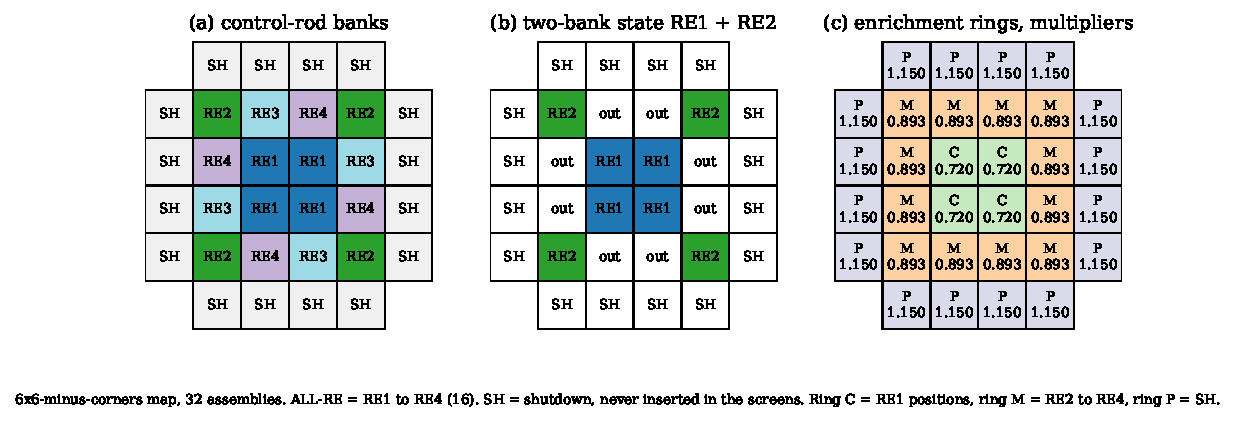
\includegraphics[width=\textwidth]{images/c8_post_core_banks_rings}
  \caption[The 32-assembly map of Campaign 8]{The 32-assembly map of Campaign 8. (a)~The four regulating banks and the shutdown bank. (b)~The two-bank state RE1 + RE2. (c)~The three enrichment rings with their multipliers.}
  \label{fig:c8-post-banks}
\end{figure}

All reactivities are quoted in pcm through the usual definition.

\begin{equation}
\rho = 10^{5}\,\frac{k - 1}{k}
\label{eq:rho-pcm}
\end{equation}

\noindent where the symbols have the following meaning.

\begin{itemize}
  \item $\rho$ is the reactivity, in pcm.
  \item $k$ is the effective multiplication factor of the core in the
        state considered, dimensionless.
\end{itemize}

The controllability screen is the one defined in
Equation~\eqref{eq:g-ctrl-meth} of Section~\ref{sec:meth-ctrl}, applied
by the evaluator on the eigenvalue itself and not on the reactivity. It
reads $k_\mathrm{RE} \leq 0.99$, that is a required margin
$\Delta k_\mathrm{margin} = 0.01$, which is \SI{1010}{pcm} on the
reactivity axis of this section.

The margin is a design reserve rather than a cited limit. It covers the
Monte Carlo uncertainty of the solve itself, which is 20 to 28\,pcm per
solve in the post-analysis, the temperature and xenon states that a
beginning-of-life eigenvalue at hot full power does not span, and the
reactivity that an operator holds in hand rather than at the point of
criticality.

Equation~\eqref{eq:g-ctrl-meth} expresses the margin in $\Delta k$, whereas
the margins reported below are reactivities, so the threshold on those
figures is $-\rho(0.99) = 1010$\,pcm rather than 1000\,pcm. No design
of the archive or of the post-analysis falls inside that 10\,pcm band,
so the two conventions separate the same designs.

\subsection{Two controllability tiers}
\label{sec:res-c8-tiers}

Feasibility in Campaign 8 is set by the four-bank screen alone. The
two-bank reading $g_\mathrm{ctrl12}$ is recorded for every design and
never constrained, so the archive can be split after the fact. Of the
19 feasible designs, four satisfy $k_\mathrm{RE12} \leq 0.99$ at
1000\,ppm, namely 12, 13, 31 and 53. None of them lies on the feasible
front. Their own front, after removing design 12, which is dominated by
53, has three members.
Table~\ref{tab:c8-post-tiers} lists both tiers and
Figure~\ref{fig:c8-post-front} places them in the objective plane.
Tier A is the feasible front and tier B the front of the designs that also
satisfy $k_\mathrm{RE12} \leq 0.99$. In the table $W_{16}$ and $W_8$ are
the beginning-of-life worths of the four regulating banks and of
RE1 + RE2. In the figure blue circles are feasible designs that need the
four regulating banks at 1000\,ppm, green squares are feasible designs
controllable with RE1 + RE2, and the two lines are the two fronts. The
error bars are one seed-to-seed standard deviation of $F_{\Delta H}$ at
the archive fidelity, about 0.011, and the dotted lines mark four and
five calendar years at 48\,MWth for an assumed capacity factor of 0.8.

\begin{table}[htbp]
  \centering
  \footnotesize
  \caption{Campaign 8 candidates in two controllability tiers, archive values at 1000\,ppm.}
  \label{tab:c8-post-tiers}
  \setlength{\tabcolsep}{3pt}\scriptsize
  \begin{tabular}{@{}c l r r r r r r r r r r r@{}}
    \toprule
    Tier & ID & $e$ & $e_\mathrm{max}$ & Gd & pins & $t_\mathrm{refl}$ & EFPD & $B_\mathrm{EOC}$ & $F_{\Delta H}$ & $k_\mathrm{core}$ & $W_{16}$ & $W_8$ \\
         &    & wt\% & wt\% & wt\% &  & cm &  & MWd/kg &  &  & pcm & pcm \\
    \midrule
    A & 47 & 4.39 & 5.05 & 2.88 & 12 & 4.29 & 1941 & 19.4 & 1.510 & 1.0981 & 17058 & 7881 \\
    A & 42 & 4.44 & 5.11 & 2.88 & 12 & 3.76 & 1968 & 19.6 & 1.522 & 1.1008 & 17035 & 7810 \\
    A & 23 & 4.94 & 5.68 & 2.80 & 12 & 4.81 & 2346 & 23.4 & 1.534 & 1.1316 & 16348 & 7596 \\
    A & 29 & 5.90 & 6.79 & 0.18 & 40 & 4.69 & 3070 & 30.6 & 1.542 & 1.1578 & 15223 & 6997 \\
    A & 21 & 7.81 & 8.99 & 3.11 & 32 & 4.92 & 4221 & 42.1 & 1.592 & 1.1264 & 14096 & 6405 \\
    A & 44 & 9.23 & 10.61 & 3.20 & 40 & 5.33 & 5019 & 50.1 & 1.612 & 1.1316 & 13178 & 5950 \\
    A & 59 & 9.34 & 10.75 & 4.32 & 40 & 5.66 & 5104 & 51.0 & 1.634 & 1.1198 & 13201 & 6014 \\
    A & 1 & 11.03 & 12.68 & 7.43 & 40 & 3.94 & 5782 & 57.7 & 1.677 & 1.1306 & 12775 & 5830 \\
    \midrule
    B & 53 & 3.45 & 3.97 & 2.92 & 12 & 4.74 & 1142 & 11.4 & 1.524 & 1.0263 & 18401 & 8384 \\
    B & 13 & 5.14 & 5.91 & 5.25 & 24 & 3.15 & 2383 & 23.8 & 1.632 & 1.0424 & 16957 & 7684 \\
    B & 31 & 6.59 & 7.58 & 3.38 & 40 & 4.18 & 3381 & 33.8 & 1.650 & 1.0339 & 15030 & 6791 \\
    \bottomrule
  \end{tabular}
\end{table}

\begin{figure}[htbp]
  \centering
  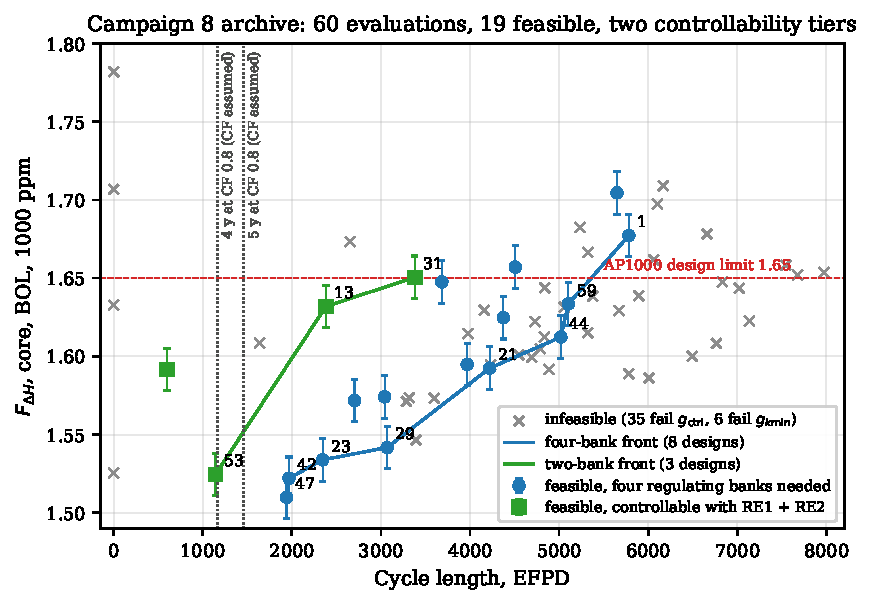
\includegraphics[width=0.9\textwidth]{images/c8_post_front_two_tier}
  \caption{The Campaign 8 archive in the objective plane, by controllability tier.}
  \label{fig:c8-post-front}
\end{figure}

Tier A is the feasible front, 47, 42, 23, 29, 21, 44, 59 and 1, from
1941 to 5782\,EFPD and $F_{\Delta H}$ from 1.510 to 1.677. Tier B is the
two-bank front, 53, 13 and 31, from 1142 to 3381\,EFPD and
$F_{\Delta H}$ from 1.524 to 1.650. At equal peaking the two-bank
requirement costs between 34 and 51\,\% of the cycle length. At
$F_{\Delta H} \approx 1.52$, tier A gives 1941 to 1968\,EFPD and tier B
gives 1142\,EFPD. At $F_{\Delta H} \approx 1.64$, tier A gives
5104\,EFPD and tier B gives 3381\,EFPD.

The two tiers are defined by the two-dimensional screen of the
campaign. The three-dimensional confirmation of
Section~\ref{sec:res-c8-3d} moves the boundary. At 1000\,ppm the
RE1 + RE2 margin of design 47 is $-1091$\,pcm on the two-dimensional
core and $+1330$\,pcm on the three-dimensional core model, and that of design 42 goes from $-1315$ to $+1052$\,pcm.
Table~\ref{tab:c8-post-3d1000} and Figure~\ref{fig:c8-post-margins1000}
show the eleven confirmed designs. In the table
$L_\mathrm{ax} = k_\mathrm{2D}/k_\mathrm{3D}$ for each rod state, the
margins are $-\rho$ of the rodded core, positive when subcritical,
$F_{\Delta H}^\mathrm{3D}$ is axially integrated, and the two-bank column
applies the screen $k_\mathrm{RE12} \leq 0.99$, that is 1010\,pcm. In the
figure dark bars are the two-dimensional core of the campaign screen and
light bars the three-dimensional core model with barrel and vessel wall, blue is the four-bank state and green the two-bank state, and the
dashed line is the screen of Equation~\eqref{eq:g-ctrl-meth}. Under the
three-dimensional reading
the two-bank set at 1000\,ppm and beginning of life is 53, 13, 31, 47
and 42, and design 23 stays out at $-1718$\,pcm. That
set is not the same as the set at the operating maximum of
Section~\ref{sec:res-c8-closures}, which is 53, 47 and 42, because the
gadolinium hump of design 31 removes \SI{4955}{pcm} of its
beginning-of-life two-bank margin of \SI{5856}{pcm} and leaves it below
the screen. Measured against
Equation~\eqref{eq:g-ctrl-meth} in its own units, design 42 satisfies the
two-bank screen by 41\,pcm, which is less than two seed standard
deviations of a single solve, so its two-bank status is not resolved by
this pair of solves. Design 47 satisfies it by 313\,pcm and is
resolved. The cost of two-bank control quoted above is
therefore a statement about the two-dimensional screen. On the
three-dimensional core it vanishes at the low-peaking floor, where
design 47 itself is two-bank controllable, and it remains 34\,\% at
$F_{\Delta H} \approx 1.64$, where design 31 stands against design 59.

\begin{table}[htbp]
  \centering
  \footnotesize
  \caption{Three-dimensional confirmation at 1000\,ppm, two seeds per solve, $150\,000 \times 200$.}
  \label{tab:c8-post-3d1000}
  \setlength{\tabcolsep}{3pt}\scriptsize
  \begin{tabular}{@{}l r r r r r r r r r r r@{}}
    \toprule
    ID & $e$ & $L_\mathrm{ax}^\mathrm{ARO}$ & $L_\mathrm{ax}^\mathrm{RE}$ & $L_\mathrm{ax}^\mathrm{RE12}$ & $M_{16}^\mathrm{2D}$ & $M_{16}^\mathrm{3D}$ & $M_8^\mathrm{2D}$ & $M_8^\mathrm{3D}$ & $F_{\Delta H}^\mathrm{2D}$ & $F_{\Delta H}^\mathrm{3D}$ & two-bank in 3D \\
       & wt\% &  &  &  & pcm & pcm & pcm & pcm &  &  &  \\
    \midrule
    53 & 3.45 & 1.0311 & 1.0177 & 1.0252 & 15857 & 17904 & 5882 & 8553 & 1.494 & 1.475 & yes \\
    47 & 4.39 & 1.0304 & 1.0163 & 1.0245 & 8123 & 9891 & -1091 & 1330 & 1.531 & 1.503 & yes \\
    42 & 4.44 & 1.0302 & 1.0162 & 1.0240 & 7894 & 9638 & -1315 & 1052 & 1.532 & 1.515 & yes \\
    23 & 4.94 & 1.0307 & 1.0161 & 1.0243 & 4759 & 6443 & -4046 & -1718 & 1.525 & 1.522 & no \\
    13 & 5.14 & 1.0301 & 1.0137 & 1.0230 & 12842 & 14388 & 3562 & 5946 & 1.603 & 1.573 & yes \\
    29 & 5.90 & 1.0303 & 1.0151 & 1.0236 & 1598 & 3136 & -6615 & -4412 & 1.527 & 1.491 & no \\
    31 & 6.59 & 1.0288 & 1.0146 & 1.0228 & 11768 & 13399 & 3491 & 5856 & 1.627 & 1.596 & yes \\
    21 & 7.81 & 1.0291 & 1.0146 & 1.0229 & 2803 & 4307 & -4776 & -2598 & 1.585 & 1.576 & no \\
    44 & 9.23 & 1.0288 & 1.0145 & 1.0226 & 1519 & 2990 & -5637 & -3508 & 1.630 & 1.600 & no \\
    59 & 9.34 & 1.0288 & 1.0145 & 1.0232 & 2502 & 3989 & -4691 & -2479 & 1.625 & 1.603 & no \\
    1 & 11.03 & 1.0286 & 1.0126 & 1.0219 & 1198 & 2470 & -5761 & -3700 & 1.673 & 1.642 & no \\
    \bottomrule
  \end{tabular}
\end{table}

\begin{figure}[htbp]
  \centering
  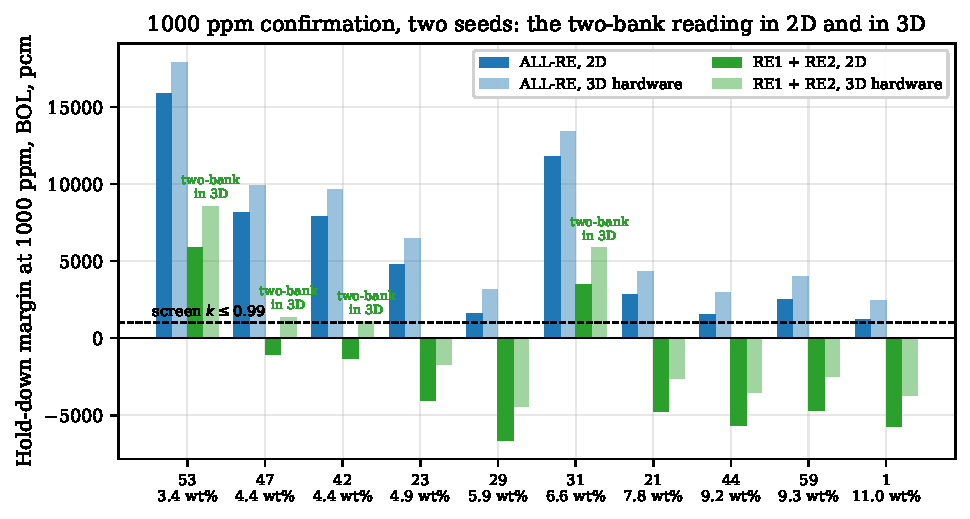
\includegraphics[width=\textwidth]{images/c8_post_margins_1000_2d3d}
  \caption{Hold-down margins at 1000\,ppm and beginning of life for the eleven confirmed designs, two seeds per solve.}
  \label{fig:c8-post-margins1000}
\end{figure}

Designs 47 and 42 are twins. They differ by 0.05\,wt\% in enrichment,
by 0.003\,wt\% in gadolinia and by 0.53\,cm in reflector thickness, and
they sit 27\,EFPD and 0.012 in $F_{\Delta H}$ apart, both within the
solve noise of Section~\ref{sec:res-c8-sigma}. The acquisition function
accepted both because the reflector thickness alone satisfied the
minimum separation of 0.14 in the normalised design space, and the
reflector is nearly inert in this box, as Section~\ref{sec:res-c8-refl}
shows. This is a limitation of separation measured in design space
rather than in objective space.

\subsection{Boron sweep}
\label{sec:res-c8-boron}

The sweep measures four quantities per design and per concentration.

\begin{equation}
M_n(c) = -\rho\!\left(k_n(c)\right)
\label{eq:margin}
\end{equation}

\noindent where the symbols have the following meaning.

\begin{itemize}
  \item $M_n(c)$ is the hold-down margin with $n$ rodded assemblies at
        boron concentration $c$, in pcm. It is positive when the rodded
        core is subcritical.
  \item $k_n(c)$ is the eigenvalue of the core with the $n$ assemblies
        rodded, dimensionless. $n = 16$ is the RE state and $n = 8$ is
        RE12.
  \item $c$ is the soluble boron concentration, in ppm.
\end{itemize}

\begin{equation}
W_n(c) = \rho\!\left(k_\mathrm{ARO}(c)\right) - \rho\!\left(k_n(c)\right)
\label{eq:bank-worth-rho}
\end{equation}

\noindent where the symbols have the following meaning.

\begin{itemize}
  \item $W_n(c)$ is the worth of the $n$ rodded assemblies at
        concentration $c$, in pcm.
  \item $k_\mathrm{ARO}(c)$ is the eigenvalue with all rods out,
        dimensionless.
\end{itemize}

Equation~\eqref{eq:bank-worth-rho} is the reactivity form of
Equation~\eqref{eq:bank-worth}, which states the same worth in units of
$k$, and it generalises it to any bank set.

The boron worth $W_B$ and the boron share $s_B$ are the quantities of
Equations~\eqref{eq:boron-worth} and~\eqref{eq:boron-share} of
Section~\ref{sec:meth-boron}, evaluated between 0 and \SI{1000}{ppm}.
The margin of Equation~\eqref{eq:margin} generalises
Equation~\eqref{eq:rod-only-margin} to a bank set of $n$ assemblies.

Table~\ref{tab:c8-post-boron} gives the results and
Figure~\ref{fig:c8-post-margin} shows the margins against
concentration. In the table $W_B$ is the differential boron worth between
0 and 1000\,ppm, and $M_{16}$ and $M_8$ are the hold-down margins under
the four regulating banks and under RE1 + RE2, positive when
subcritical. $c_8$ and $c_{16}$ are the boron concentrations at which the
two margins reach the screen value $k \leq 0.99$, that is 1010\,pcm, by
linear interpolation between the sweep points, and entries marked e are
extrapolated beyond 1500\,ppm. In the figure the left panel holds the
four regulating banks and the right panel RE1 + RE2, solid lines are
front members, dashed lines are the retained two-bank designs, and the
dashed horizontal line is the screen of Equation~\eqref{eq:g-ctrl-meth}.
Three regularities stand out.

\begin{table}[htbp]
  \centering
  \footnotesize
  \caption{Boron sweep of the eleven designs, two-dimensional core, one seed, $150\,000$ particles and 200 batches.}
  \label{tab:c8-post-boron}
  \setlength{\tabcolsep}{2.5pt}\scriptsize
  \begin{tabular}{@{}l l r r r r r r r r r@{}}
    \toprule
    ID & set & $W_B$ & $M_{16}(0)$ & $M_{16}(1000)$ & $M_8(1000)$ & $M_8(1500)$ & $c_{16}$ & $c_8$ & $W_8/W_{16}$ & share \\
       &     & pcm/ppm & pcm & pcm & pcm & pcm & ppm & ppm &  &  \\
    \midrule
    53 & two-bank & 8.54 & 7537 & 15881 & 5867 & 9958 & 0 & 415 & 0.457 & 0.317 \\
    47 & front & 6.98 & 1382 & 8144 & -1053 & 2212 & 0 & 1316 & 0.461 & 0.290 \\
    42 & front & 6.88 & 1225 & 7946 & -1287 & 1977 & 0 & 1352 & 0.460 & 0.287 \\
    23 & front & 6.31 & -1308 & 4745 & -4068 & -1119 & 380 & 1861e & 0.461 & 0.278 \\
    13 & two-bank & 6.14 & 7022 & 12937 & 3581 & 6420 & 0 & 566 & 0.448 & 0.266 \\
    29 & front & 5.22 & -3452 & 1574 & -6643 & -4156 & 886 & 2539e & 0.459 & 0.256 \\
    31 & two-bank & 4.79 & 7221 & 11832 & 3455 & 5763 & 0 & 472 & 0.446 & 0.241 \\
    21 & front & 4.18 & -1180 & 2877 & -4783 & -2851 & 533 & 2499e & 0.455 & 0.229 \\
    44 & front & 3.50 & -1816 & 1523 & -5678 & -3914 & 846 & 2895e & 0.453 & 0.210 \\
    59 & front & 3.54 & -835 & 2477 & -4677 & -3013 & 551 & 2709e & 0.456 & 0.212 \\
    1 & front & 3.13 & -1682 & 1228 & -5764 & -4293 & 926 & 3302e & 0.453 & 0.197 \\
    \bottomrule
  \end{tabular}
\end{table}

\begin{enumerate}
  \item The two-bank worth is a fixed fraction of the four-bank worth.
        Over the eleven designs $W_8 / W_{16}$ lies between 0.446 and
        0.461, and over all 60 archive designs it is $0.458 \pm 0.007$.
        The fraction does not depend on enrichment, gadolinia loading or
        reflector thickness. It is a property of the map of
        Figure~\ref{fig:c8-post-banks}, in which RE1 and RE2 occupy the
        eight positions of highest importance.

  \item Both the bank worth and the boron worth fall with enrichment.
        $W_{16}$ at 1000\,ppm decreases from 18\,401\,pcm at 3.45\,wt\% to
        12\,775\,pcm at 11.0\,wt\%, with a correlation of $-0.95$ with
        enrichment across the archive. The differential boron worth
        decreases from 8.54 to 3.13\,pcm/ppm over the same range. Both
        follow the hardening of the spectrum.

  \item Boron carries a minority of the hold-down capacity. The share
        $s_B$ lies between 0.197 and 0.317. At 1000\,ppm the four
        regulating banks carry between 68 and 80\,\% of the beginning-of-life
        hold-down of every candidate.
\end{enumerate}

\begin{figure}[htbp]
  \centering
  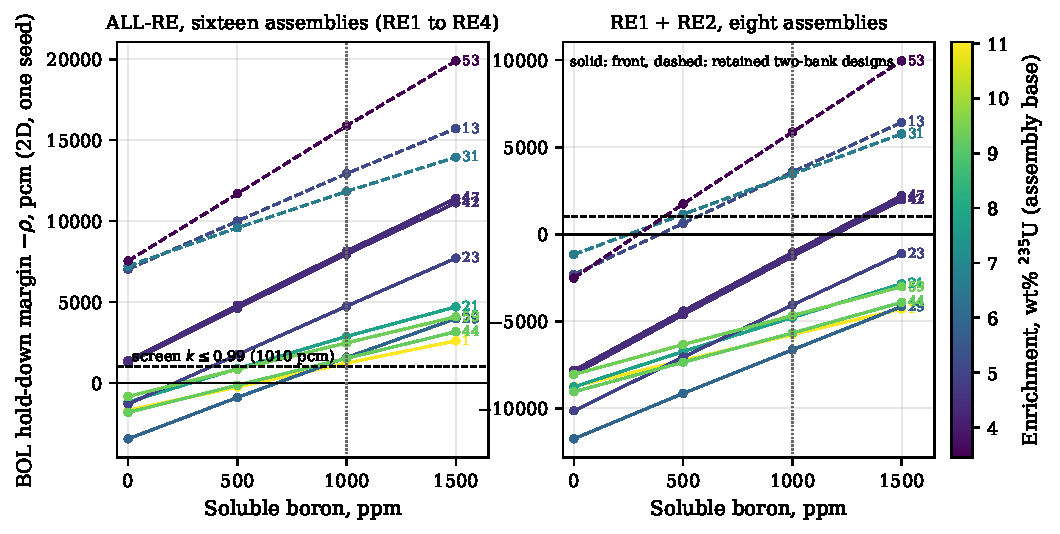
\includegraphics[width=\textwidth]{images/c8_post_margin_vs_boron}
  \caption{Beginning-of-life hold-down margin against soluble boron for the eleven designs, two-dimensional core, one seed.}
  \label{fig:c8-post-margin}
\end{figure}

The first regularity makes the two-bank margin predictable from the
four-bank one.

\begin{equation}
M_8(c) \approx M_{16}(c) - \left(1 - r\right) W_{16}(c)
\label{eq:m8-from-m16}
\end{equation}

\noindent where the symbols have the following meaning.

\begin{itemize}
  \item $M_8(c)$ and $M_{16}(c)$ are the margins of
        Equation~\eqref{eq:margin}, in pcm.
  \item $W_{16}(c)$ is the four-bank worth of
        Equation~\eqref{eq:bank-worth-rho}, in pcm.
  \item $r$ is the ratio $W_8 / W_{16}$, equal to 0.458 for this map,
        dimensionless.
\end{itemize}

Read through the boron concentration, the sweep gives the concentration
at which each design reaches the screen of Equation~\eqref{eq:g-ctrl-meth}
with eight rods, by linear interpolation between the sweep points.
Figure~\ref{fig:c8-post-boron} shows it, with the values that lie beyond
the 1500\,ppm sweep point marked as extrapolated. The three tier B designs reach
it at 415, 472 and 566\,ppm. The twins 47 and 42 reach it at 1316 and
1352\,ppm, about 35\,\% above the screen value. The remaining front
members need 1861 to 3302\,ppm, the last four by extrapolation beyond
the sweep. The screen at 1000\,ppm is therefore a modelling choice that
separates the front from two-bank control by a margin that the twins
could close with a higher beginning-of-cycle concentration, whereas the
long-cycle designs could not within any concentration used at power.
%% AUTHOR: state here the beginning-of-cycle boron concentrations of the
%% reference designs already cited in sec:meth-boron-basis, so that the
%% 1300 to 1350 ppm of the twins is placed against a cited range rather
%% than against a general statement.

\begin{figure}[htbp]
  \centering
  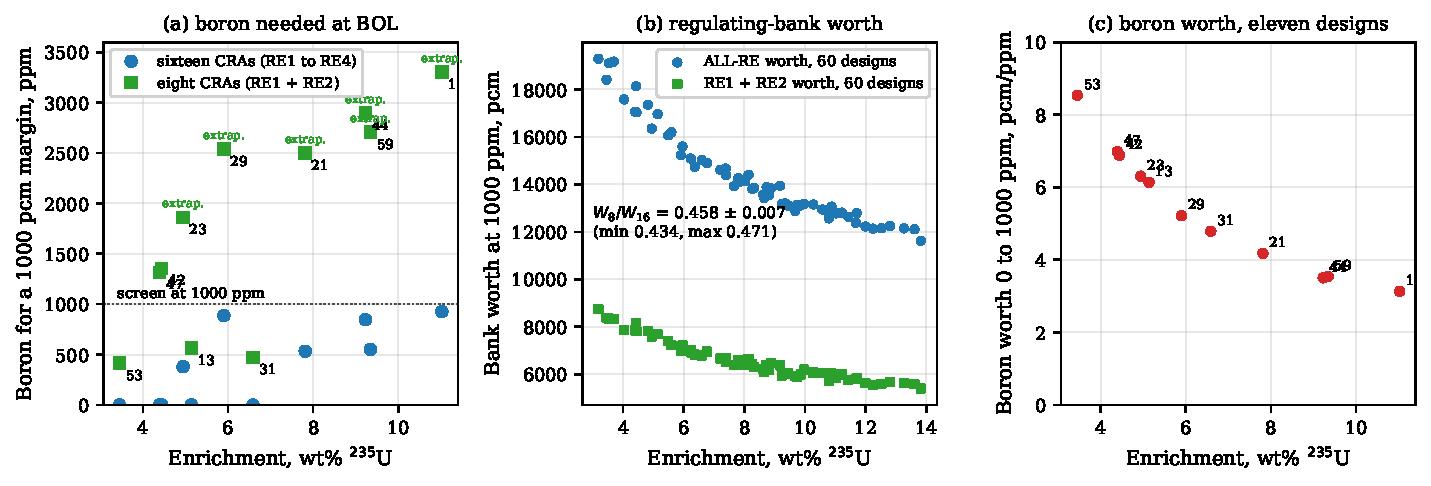
\includegraphics[width=\textwidth]{images/c8_post_boron_required_and_worths}
  \caption[Soluble boron and bank worths of the Campaign 8 designs]{Soluble boron and bank worths. (a)~Soluble boron needed at beginning of life for the screen margin with sixteen and with eight rodded assemblies, eleven designs. (b)~Four-bank and two-bank worth at 1000\,ppm, 60 archive designs. (c)~Differential boron worth, eleven designs.}
  \label{fig:c8-post-boron}
\end{figure}

The sweep closes on the archive. At 1000\,ppm the sweep eigenvalues
differ from the archive values by $-72$ to $+50$\,pcm over the 33
comparisons, with the archive solves at $100\,000 \times 170$ particles
and batches and the sweep at $150\,000 \times 200$.

\subsection{Zero-boron hold-down by the regulating banks}
\label{sec:res-c8-zeroboron}

Stage D asks whether the four regulating banks alone hold the
beginning-of-life core subcritical with no soluble boron, on the
two-dimensional core and on the three-dimensional core with the
benchmark rod stack. Table~\ref{tab:c8-post-zeroboron} and
Figure~\ref{fig:c8-post-zero} give the result. In the table
$L_\mathrm{ax}$ is $k_\mathrm{2D}/k_\mathrm{3D}$ for the rodded state with
the benchmark rod stack: bottom 12.04\,cm unrodded, 30.48\,cm Ag-In-Cd and
77.48\,cm B$_4$C. In the figure grey is the one-seed sweep, blue the
two-seed two-dimensional solve of stage D and orange the three-dimensional core model with the axial structures of the assemblies, barrel and vessel wall. Green markers meet the screen $k \leq 0.99$, orange markers are
subcritical below it and red markers are supercritical. The condition
tested is
the following.

\begin{table}[htbp]
  \centering
  \footnotesize
  \caption{Zero-boron hold-down by the four regulating banks alone at beginning of life, stage D, two seeds per solve.}
  \label{tab:c8-post-zeroboron}
  \begin{tabular}{@{}l r r r r r r l@{}}
    \toprule
    ID & $e$ & $k_\mathrm{2D}$ & $k_\mathrm{3D}$ & $M_{16}^\mathrm{2D}$ & $M_{16}^\mathrm{3D}$ & $L_\mathrm{ax}$ & reading \\
       & wt\% &  &  & pcm & pcm &  &  \\
    \midrule
    53 & 3.45 & 0.9301 & 0.9134 & 7518 & 9486 & 1.0183 & holds with margin \\
    47 & 4.39 & 0.9860 & 0.9702 & 1419 & 3069 & 1.0163 & holds with margin \\
    42 & 4.44 & 0.9872 & 0.9724 & 1301 & 2841 & 1.0152 & holds with margin \\
    23 & 4.94 & 1.0130 & 0.9966 & -1281 & 341 & 1.0164 & subcritical, margin < 1000 \\
    13 & 5.14 & 0.9346 & 0.9220 & 6996 & 8454 & 1.0136 & holds with margin \\
    29 & 5.90 & 1.0356 & 1.0201 & -3440 & -1967 & 1.0153 & supercritical \\
    31 & 6.59 & 0.9325 & 0.9201 & 7237 & 8684 & 1.0135 & holds with margin \\
    21 & 7.81 & 1.0110 & 0.9968 & -1089 & 318 & 1.0142 & subcritical, margin < 1000 \\
    44 & 9.23 & 1.0187 & 1.0048 & -1839 & -476 & 1.0139 & supercritical \\
    59 & 9.34 & 1.0086 & 0.9942 & -853 & 581 & 1.0145 & subcritical, margin < 1000 \\
    1 & 11.03 & 1.0173 & 1.0049 & -1699 & -491 & 1.0123 & supercritical \\
    \bottomrule
  \end{tabular}
\end{table}

\begin{equation}
k_\mathrm{RE}^\mathrm{3D}(0) \leq 1 - \Delta k_\mathrm{margin} = 0.99
\label{eq:boronfree-necessary}
\end{equation}

\noindent where the symbols have the following meaning.

\begin{itemize}
  \item $k_\mathrm{RE}^\mathrm{3D}(0)$ is the
        beginning-of-life eigenvalue of the three-dimensional core with
        the four regulating banks inserted and no soluble boron,
        dimensionless.
  \item $\Delta k_\mathrm{margin}$ is the margin of
        Equation~\eqref{eq:g-ctrl-meth}, equal to $0.01$, dimensionless. On
        the reactivity axis of Figure~\ref{fig:c8-post-zero} the
        condition reads $M_{16}^\mathrm{3D}(0) \geq 1010$\,pcm.
\end{itemize}

\begin{figure}[htbp]
  \centering
  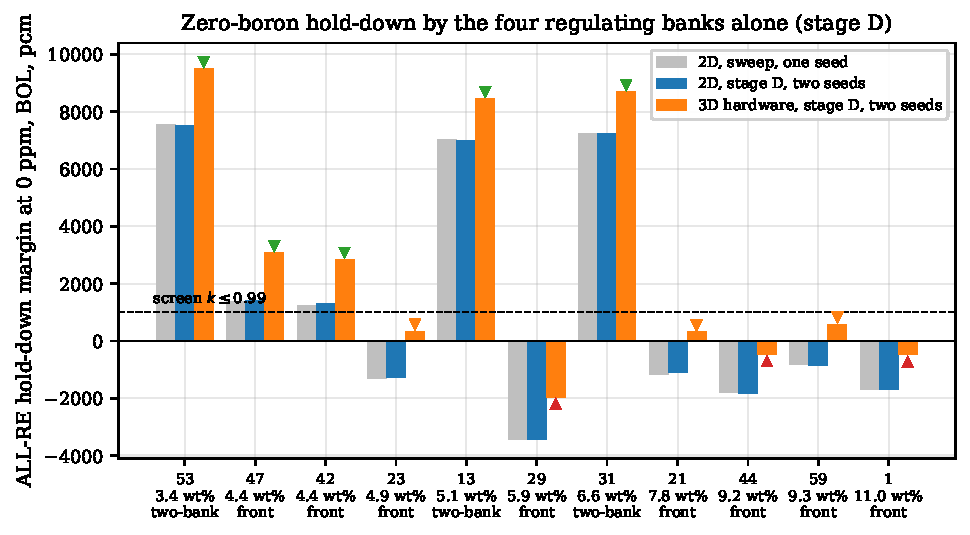
\includegraphics[width=\textwidth]{images/c8_post_zero_boron_margin}
  \caption{Zero-boron hold-down margin under the four regulating banks at beginning of life.}
  \label{fig:c8-post-zero}
\end{figure}

Five designs meet the condition. The three tier B designs hold with
8454 to 9486\,pcm, and the twins 47 and 42 hold with 3069 and
2841\,pcm. Three front members, 23, 21 and 59, are subcritical by only
318 to 581\,pcm, below the margin. Three front members, 29, 44 and 1,
are supercritical under the four banks without boron. No design is
subcritical under RE1 + RE2 alone at 0\,ppm, the two-bank margin there
being $-1162$ to $-11\,757$\,pcm.

Two members of the feasible front satisfy
Equation~\eqref{eq:boronfree-necessary}, designs 47 and 42, at
\SI{3069}{pcm} and \SI{2841}{pcm}. Of the two, design 47 is the
candidate carried forward, because it is also the low-peaking floor of
the front and the only one of the pair whose two-bank status is
resolved beyond the seed uncertainty
(Section~\ref{sec:res-c8-3d}). It is therefore the boron-bearing
candidate of tier A and, at the same time, the design on which a
boron-free variant of the core can be studied.

The three tier B designs hold at zero boron by a wider margin than
either front member, \SIrange{8454}{9486}{pcm} against
\SIrange{2841}{3069}{pcm}, so the design best placed for a boron-free
study is not on the front at all. This is the same inversion reported
in Section~\ref{sec:res-c8-tiers} for controllability, seen now in the
boron budget.

Two limits apply to every statement in this subsection.
Equation~\eqref{eq:boronfree-necessary} is a necessary condition and
not a demonstration, and three things it does not cover are listed in
Section~\ref{sec:res-c8-post-limits}. It is also a four-bank condition
throughout: no design of the eleven is subcritical under RE1 + RE2
alone at \SI{0}{ppm}, so none of these designs is boron-free on the
two-bank state that tier B is defined by.

The one-seed sweep and the two-seed two-dimensional solve agree within
100\,pcm for every design. The three-dimensional core adds 1207 to
1968\,pcm of margin in the rodded state, which is the axial factor of
the rodded core discussed in Section~\ref{sec:res-c8-3d}.

\subsection{Which constraint binds}
\label{sec:res-c8-nesting}

In Campaign 7 the derived ceiling $k_{\max}$ rejected fourteen
controllable designs and the control screen rejected none that the
ceiling accepted. Campaign 8 inverts this. Of the 41 infeasible designs,
six fail $k_{\min}$, 23 fail both $k_{\max}$ and the control screen, and
twelve fail the control screen alone. No design fails $k_{\max}$ alone.
The three-dimensionally derived ceiling of 1.166 is now a redundant
outer bound and the control screen is the binding constraint.
Figure~\ref{fig:c8-post-nesting} shows the structure. In panel~(a) the
twelve designs rejected by the control screen alone are circled in red.
The dashed line is the screen value 0.99, and the dotted lines are
$k_{\min}$ and $k_{\max}$.

\begin{figure}[htbp]
  \centering
  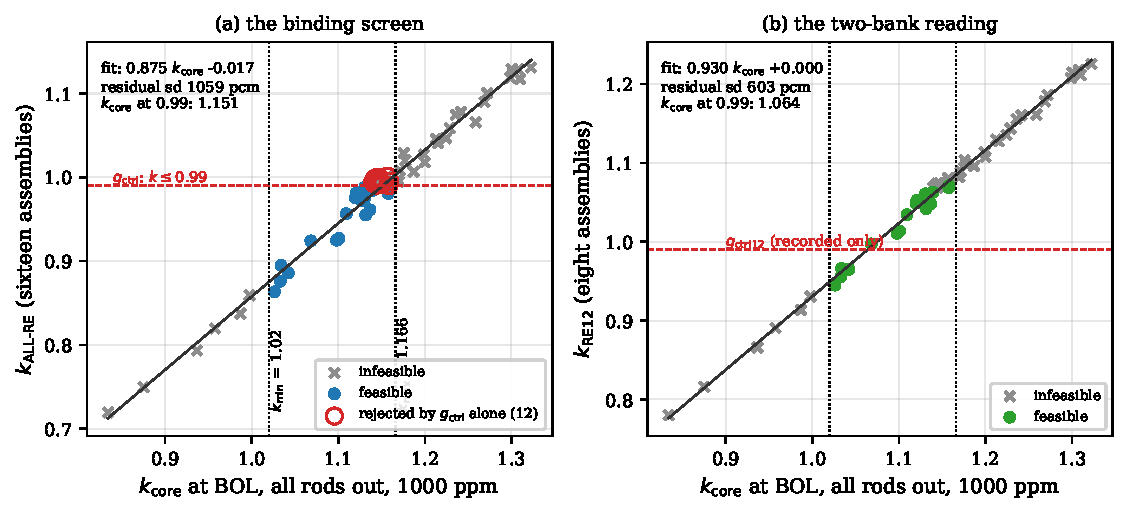
\includegraphics[width=\textwidth]{images/c8_post_constraint_structure}
  \caption[Rodded against unrodded core eigenvalues of the Campaign 8 archive]{Rodded against unrodded core eigenvalues of the 60 Campaign 8 archive designs at 1000\,ppm. (a)~Four-bank state. (b)~Two-bank state.}
  \label{fig:c8-post-nesting}
\end{figure}

A linear fit across the archive gives
$k_\mathrm{RE} = 0.875\,k_\mathrm{core} - 0.017$ with a
residual standard deviation of 1059\,pcm, so the control screen acts
as an effective ceiling near $k_\mathrm{core} = 1.151$, with a spread
that the bank worth of each design sets. For the two-bank state the fit
is $k_\mathrm{RE12} = 0.930\,k_\mathrm{core}$ with a residual of
603\,pcm, and the effective ceiling is $k_\mathrm{core} = 1.064$.

\subsection{Statistical resolution of the front}
\label{sec:res-c8-sigma}

The post-analysis ran every solve with two seeds and the marginal
re-score with three. Table~\ref{tab:c8-post-sigma} pools the seed-to-seed
standard deviations. For the eigenvalue it is 20 to 23\,pcm, equal to
the Monte Carlo standard deviation reported by each solve, so the
reported uncertainty is faithful. For the peaking factor it is 0.011 with
all rods out on the two-dimensional core, pooled over fourteen pairs,
0.012 on the three-dimensional core, whose value is axially integrated,
and 0.024 to 0.029 in the rodded states, whose power distribution is
far more peaked.

\begin{table}[htbp]
  \centering
  \footnotesize
  \caption{Seed-to-seed standard deviation of the post-analysis core solves at $150\,000$ particles, 200 batches and 80 inactive batches.}
  \label{tab:c8-post-sigma}
  \begin{tabular}{@{}l l r r r@{}}
    \toprule
    State & Model & pairs & $\sigma_\mathrm{seed}(k)$, pcm & $\sigma_\mathrm{seed}(F_{\Delta H})$ \\
    \midrule
    RE, 0 ppm & 2D & 11 & 20 & 0.0278 \\
    RE, 0 ppm & 3Dhw & 11 & 23 & 0.0273 \\
    ARO, 1000 ppm & 2D & 14 & 14 & 0.0106 \\
    ARO, 1000 ppm & 3Dhw & 14 & 24 & 0.0119 \\
    \bottomrule
  \end{tabular}
\end{table}

Scaled to the archive fidelity of $100\,000 \times 170$, the
seed-to-seed standard deviation of $F_{\Delta H}$ is about 0.014. The
low-peaking end of the front, designs 47, 42, 23 and 29, spans 1.510 to
1.542 in steps of 0.008 to 0.012, less than one standard deviation
each. These four designs are ordered by cycle length but not by
peaking. Any statement that ranks them by $F_{\Delta H}$ requires a
replicate of at least four seeds at 1000\,ppm with all rods out, which
brings the standard error of each mean to about 0.006, the size of the
smallest step.

The re-score of designs 54 and 11 with three seeds gives
$k_\mathrm{RE} = 0.99038 \pm 54$ and $0.99053 \pm 25$\,pcm.
Both are subcritical and both remain above the screen value 0.99, by
38 and 53\,pcm, so the feasibility count stays at 19. Both are dominated
on the objectives, 54 by 21 and 44, and 11 by 44, so the front is
unchanged either way.

\subsection{Three-dimensional closures}
\label{sec:res-c8-3d}

The axial factor of the rodded core differs from that of the unrodded
core. With all rods out the three-dimensional core model gives
$L_\mathrm{ax} = k_\mathrm{2D} / k_\mathrm{3D}$ between 1.0286 and
1.0311 at 1000\,ppm over the eleven confirmed designs, against the 1.0282
to 1.0298 of the water-slab axial study of Section~\ref{sec:meth-lax}.
With RE1 + RE2 inserted it is between 1.0219 and 1.0252, and with the
four regulating banks inserted between 1.0126 and 1.0177. The reason is
the rod stack.
The two-dimensional screen inserts B$_4$C over the whole fuel height,
whereas the benchmark rod leaves the bottom 12.04\,cm of the fuel
unrodded, carries 30.48\,cm of Ag-In-Cd above it and B$_4$C over the
remaining 77.48\,cm. The three-dimensional rodded core is therefore
less rodded than the two-dimensional one, and part of the axial leakage
gain is spent on the weaker stack, in proportion to the number of rods
inserted. The two-dimensional control screen remains conservative, by
\num{1272} to \SI{2047}{pcm} for the four-bank state and by \num{2062}
to \SI{2671}{pcm} for the two-bank state, rather than by the 2900 to
3100\,pcm that the unrodded axial factor would suggest. Both ranges are
the differences of the margin columns of
Table~\ref{tab:c8-post-3d1000} over the eleven confirmed designs. The
two-dimensional eigenvalues of the confirmation reproduce the archive
within $-53$ to $+69$\,pcm over the thirty-three comparisons.

The unrodded axial factor splits by enrichment. The six designs at or
below \SI{5.90}{wt\%} give 1.0301 to 1.0311 and the five at or above
\SI{6.59}{wt\%} give 1.0286 to 1.0291. The campaign value 1.0289 is
therefore right for the long-cycle designs and 120 to 220\,pcm low for
the low-peaking end of the front.
%% AUTHOR: physics of the split. Two mechanisms are candidates, the
%% parked-rod plug at the fuel top weighing more where the competing
%% absorption is lower, and the migration area of the softer spectrum.
%% Stage E on design 47 isolates the first at 129 pcm, so the second
%% accounts for the remainder of the 130 to 220 pcm. State which you
%% adopt, or leave the observation as measured.

The parked rods matter. With the withdrawn rods removed from the model,
design 47 gives $L_\mathrm{ax} = 1.0291$, within 20\,pcm of the
campaign value 1.0289 taken from the water-slab axial study. With the
rods parked in the benchmark position the factor is 1.0304, a
difference of 129\,pcm, because the withdrawn rod leaves its steel end
plug in the top 4.86\,cm of the fuel and its Ag-In-Cd tip in the
plenum above. The parked geometry therefore raises the end-of-cycle
target by about 130\,pcm, which shortens the reported cycle of design
47 by about 24\,EFPD, or 1.2\,\%, on the slope of its reactivity
history, and the long cycles by a smaller fraction.

The downcomer trade is nearly free. Thinning the reflector of designs
47, 21 and 59 to 3.969\,cm, which gives a 3.7\,cm downcomer at the
1.26\,cm pitch, changes the unrodded two-dimensional eigenvalue by
$-5$, $-95$ and $-128$\,pcm and the peaking factor by $+0.003$ to
$+0.005$, below one seed standard deviation.
Table~\ref{tab:c8-post-downcomer} gives the values. The native column
is the archive core solve at $100\,000 \times 170$, and $\Delta\rho$ is
the reactivity change of the two-dimensional core. A downcomer of
3.7\,cm can be adopted for every candidate at a cost of at most
130\,pcm at beginning of life.

\begin{table}[htbp]
  \centering
  \footnotesize
  \caption{Stage G: reflector thinned to 3.969\,cm for a 3.7\,cm downcomer at pitch 1.26\,cm, all rods out, 1000\,ppm, two seeds.}
  \label{tab:c8-post-downcomer}
  \setlength{\tabcolsep}{3pt}\scriptsize
  \begin{tabular}{@{}l r r r r r r r@{}}
    \toprule
    ID & $t_\mathrm{refl}$ & downcomer & $k_\mathrm{2D}$ & $k_\mathrm{2D}$ & $\Delta\rho$ & $F_{\Delta H}$ & $F_{\Delta H}$ \\
       & native, cm & native, cm & native & at 3.969 & pcm & native & at 3.969 \\
    \midrule
    47 & 4.29 & 3.38 & 1.0981 & 1.0980 & -4 & 1.510 & 1.513 \\
    21 & 4.92 & 2.75 & 1.1264 & 1.1253 & -82 & 1.592 & 1.595 \\
    59 & 5.66 & 2.01 & 1.1198 & 1.1186 & -102 & 1.634 & 1.639 \\
    \bottomrule
  \end{tabular}
\end{table}

\subsection{The reflector inside the Campaign 8 box}
\label{sec:res-c8-refl}

Campaign 3 found the radial peaking of the core to fall with reflector
thickness over the 2 to 19.5\,cm range. Inside the 2.0 to 5.66\,cm box
of Campaign 8 the effect is not resolved. A multiple regression of
$F_{\Delta H}$ on the four design variables over the 60 designs gives
$-0.0085$ per centimetre, that is $-0.031$ across the box, and the
subset below 7\,wt\% gives the opposite sign. The direct test of
Section~\ref{sec:res-c8-3d} measures at most $+0.005$ for a thinning of
0.3 to 1.7\,cm. Figure~\ref{fig:c8-post-refl} shows both, with the
designs coloured by enrichment, circles for the feasible designs and red
arrows for the stage G solves with the reflector thinned to 3.969\,cm.

\begin{figure}[htbp]
  \centering
  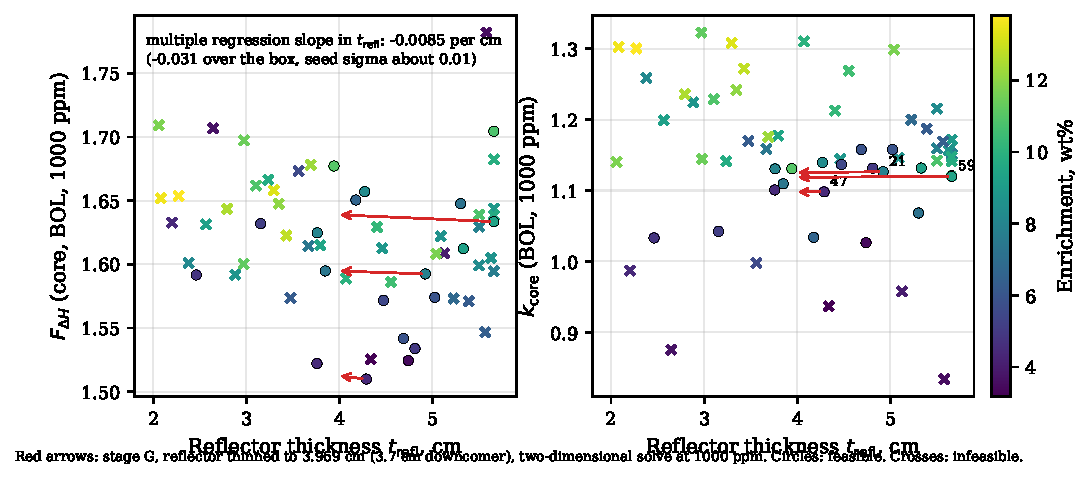
\includegraphics[width=\textwidth]{images/c8_post_reflector_leverage}
  \caption{Peaking factor and unrodded core eigenvalue against reflector thickness, 60 Campaign 8 archive designs.}
  \label{fig:c8-post-refl}
\end{figure}

Within this box the reflector thickness is therefore nearly inert. It
carries about 52\,pcm per centimetre of reactivity through the target of
Section~\ref{sec:meth-lax} and a peaking effect of the order of the
solve noise. Two consequences follow.

\begin{enumerate}
  \item The infill separation criterion, measured in the normalised
        design space, admitted the twins 47 and 42 on the strength of
        the reflector coordinate alone. A separation criterion in
        objective space, or a smaller weight on inert coordinates, would
        have spent that evaluation elsewhere.

  \item Any further campaign in this box should fix the reflector at
        3.97\,cm, which gives the 3.7\,cm downcomer, and search the three
        active variables.
\end{enumerate}

\subsection{Moderator temperature coefficient and the boron ceiling}
\label{sec:res-c8-mtc}

The boron sweep and the swing table give the critical concentration of
each candidate, and Section~\ref{sec:meth-mtc} defines the ceiling that
concentration has to stay below at power. The ceiling was measured on
C8-47, and Table~\ref{tab:c8-mtc} gives its two-dimensional screen and
its value on the three-dimensional core model at the two primary
conditions.

\begin{table}[htbp]
  \centering
  \small
  \caption{C8-47, zoned core: soluble boron ceiling at two primary conditions.}
  \label{tab:c8-mtc}
  \begin{tabular}{@{}rcrrrr@{}}
    \toprule
    Pressure & Bracket & 2D screen & 3D result & 3D weighted fit & 3D margin on 2327\,ppm \\
    {[MPa]} & [K] & [ppm] & [ppm] & [ppm] & [ppm] \\
    \midrule
    15.5 & 570 to 590 & 2336 & 2997 & $2981 \pm 61$ & $+670$ \\
    12.8 & 547 to 567 & 2255 & 2763 & $2762 \pm 70$ & $+436$ \\
    \bottomrule
  \end{tabular}
\end{table}

The ceilings are the two-point values of Section~\ref{sec:meth-mtc}, and
a weighted linear fit over the scanned concentrations agrees with the
three-dimensional values within one standard deviation at both
pressures. The Doppler coefficient is negative and resolved throughout,
from $-2.15$ to \SI{-1.79}{pcm} per K at \SI{15.5}{MPa} and from
$-2.08$ to \SI{-1.85}{pcm} per K at \SI{12.8}{MPa}, so the temperature
interpolation is active. The axial leakage contribution of
Equation~\eqref{eq:axial-feedback} is $-10.63 \pm 0.55$\,pcm per K, 29
per cent of the total coefficient of the three-dimensional core at the
conditions of the scan, and it raises the ceiling by \SI{661}{ppm} at
\SI{15.5}{MPa} and by \SI{508}{ppm} at \SI{12.8}{MPa}.

Design 47 itself needs \SI{2327}{ppm} at beginning of life, measured
as the root of its zoned reactivity curve at \SI{570}{K} with the
state offset of \SI{157}{pcm} between the scan and the campaign
operating point applied. The linear estimate of
Table~\ref{tab:c8-swing} is \SI{2348}{ppm}. Its hump is negative, so
beginning of life is its most reactive state, and it clears the
three-dimensional ceiling by \SI{670}{ppm} at \SI{15.5}{MPa} and
\SI{436}{ppm} at \SI{12.8}{MPa}. Under the two-dimensional screen it is
marginal at \SI{15.5}{MPa}, \SI{9}{ppm} below 2336, and fails at
\SI{12.8}{MPa}, \SI{72}{ppm} above 2255, a difference that the axial
term of Section~\ref{sec:meth-mtc-3d} accounts for. The estimates of Table~\ref{tab:c8-swing} place the
other candidates as follows, with the caution that the ceiling was
measured on the lattice of design 47 only.

\begin{enumerate}
  \item Designs 53, 13 and 42 need 1312, 1697 and \SI{2377}{ppm}, all
        with a negative hump, and lie below both ceilings. A second
        record of design 13 gives \SI{1701}{ppm}, a difference below
        the resolution of the estimate.

  \item Design 31 needs \SI{1701}{ppm} at beginning of life and
        \SI{2760}{ppm} at the maximum of its hump, \SI{3}{ppm} below the
        three-dimensional ceiling at \SI{12.8}{MPa}.

  \item Design 23 needs \SI{2979}{ppm}, \SI{18}{ppm} below the
        three-dimensional ceiling at \SI{15.5}{MPa} and above the one at
        \SI{12.8}{MPa}.

  \item The five long-cycle members of the front, 29, 21, 59, 44 and 1,
        need 3677 to \SI{4674}{ppm} at beginning of life, above both
        ceilings.
\end{enumerate}

Boron control at a non-positive coefficient is therefore available to
the short-cycle end of the front and to the two-bank subset, and not
to the long-cycle designs. This is the same division that the
controllability readings of Sections~\ref{sec:res-c8-tiers}
and~\ref{sec:res-c8-zeroboron} drew.

\subsection{The proxy gap on the zoned core}
\label{sec:res-proxy-gap-zoned}

The bridge model of Equation~\eqref{eq:bridge} was fitted in
Section~\ref{sec:res-corevalidation} on the uniform-loading archive of
Campaign~3, where it identified the reflector thickness and the pin
pitch as the variables that set the ratio between the core and the
assembly peaking factor. From Campaign~6 the evaluator builds the zoned
core of Section~\ref{sec:meth-zoning}, and every archive from
Campaign~4 onward stores both peaking factors of each design, the core
value as the objective and the assembly value as the diagnostic of
Section~\ref{sec:meth-core-objective}. The fit can therefore be
repeated on the zoned core without new transport.

Table~\ref{tab:proxy-gap-zoned} compares the four archives. The
Campaign~3 row is not a sample mean: it is
Equation~\eqref{eq:bridge-fit} evaluated at the operating point of
Campaign~8, $p = \SI{1.26}{cm}$ and $t_\mathrm{refl} = \SI{4.0}{cm}$.
The regression cannot be fitted on the Campaign~8 archive, whose pitch
is fixed, so only the mean ratio is given for it. The zoned ratios were
computed from the archived core and assembly peaking factors of the
Campaign~6, 7 and 8 checkpoints.

\begin{table}[htbp]
  \centering
  \small
  \caption{Uniform and zoned archives: ratio of the core to the assembly peaking factor.}
  \label{tab:proxy-gap-zoned}
  \begin{tabular}{@{}llrcrr@{}}
    \toprule
    Archive & Loading & $n$ & Pitch & $F_{\Delta H}^\mathrm{core}/F_{\Delta H}^\mathrm{asm}$ & $R^2$ of \\
     &  &  & [cm] & mean $\pm$ sd & Eq.~\eqref{eq:bridge} \\
    \midrule
    Campaign 3 & uniform & 36  & 1.15 to 1.43 & 1.814 (fit) & 0.746 \\
    Campaign 6 & zoned   & 114 & 1.15 to 1.43 & $1.318 \pm 0.052$ & 0.030 \\
    Campaign 7 & zoned   & 60  & 1.15 to 1.41 & $1.297 \pm 0.035$ & 0.052 \\
    Campaign 8 & zoned   & 60  & 1.26 fixed   & $1.313 \pm 0.029$ & -- \\
    \bottomrule
  \end{tabular}
\end{table}

Three readings follow.

\begin{enumerate}
  \item The ratio is much smaller on the zoned core. The Campaign~3 fit
        predicts 1.814 at the Campaign~8 operating point, and the
        Campaign~8 archive gives 1.313. The quotient of the two, 1.38,
        lies within the peaking reduction measured directly on two
        Campaign~5 champions in Table~\ref{tab:zoning-confirm}, where
        zoning lowered $F_{\Delta H}$ from 2.026 to 1.501 and from 2.043
        to 1.473, factors of 1.35 and 1.39. The archive comparison and
        the controlled comparison give the same zoning benefit.

  \item The geometric dependence is lost. On the uniform core the two
        regressors of Equation~\eqref{eq:bridge} explain three quarters
        of the variance of the ratio. On the Campaign~6 archive, over
        the same pitch range and with three times as many designs, they
        explain 3 per cent, and 5 per cent on Campaign~7. Within its
        scatter, the ratio on the zoned core depends on neither the
        reflector thickness nor the pitch.

  \item The ratio is stable between campaigns. The three zoned archives
        give 1.318, 1.297 and 1.313, a spread of 0.021, smaller than
        the standard deviation within each archive, 0.029 to 0.052,
        over 234 designs and three different design spaces.
\end{enumerate}

The zoning was designed to remove this dependence. The assembly
calculation has reflective boundaries, so it describes an infinite
lattice of identical assemblies and measures only the pin-to-pin
structure inside one assembly, 1.14 to 1.15 on the uniform Campaign~3
finalists of Table~\ref{tab:core-finalists}. The core calculation keeps
that structure and multiplies it, approximately, by the radial form
factor, the ratio of the power of the hottest assembly to the core
mean. On the uniform core the form factor is large and depends on the
geometry, because the reflector and the pitch set how steeply the power
falls toward the periphery. The zoned map enriches the periphery and
derates the centre while the fissile balance of
Equation~\eqref{eq:zoning-balance} holds the mean multiplier at one,
and the form factor that results is smaller and insensitive to the two
geometric variables.

Two consequences follow for the method.

\begin{enumerate}
  \item The Campaign~4 decision to measure the core peaking inside the
        loop holds on the zoned core as well. A constant ratio with a
        relative scatter of 2.2 per cent on Campaign~8 corresponds to
        about 0.036 in the core peaking factor. That is between two and
        three times the seed-to-seed standard deviation of the core
        solve at the archive fidelity, about 0.014
        (Section~\ref{sec:res-c8-sigma}), and larger than the steps of
        0.008 to 0.012 between the low-peaking designs of the front. A
        corrected assembly value would place a design in the right
        region of the objective plane but could not order the front on
        the peaking axis, and at 3 per cent of an evaluation the
        measurement is the cheaper choice.

  \item Outside the loop, for screening, the assembly peaking predicts
        the core peaking of the zoned core through a single calibrated
        factor. The leakage-corrected reactivity target of
        Section~\ref{sec:meth-ktarget} has the same property for the
        multiplication factor: an assembly calculation carries the core
        behaviour once a correction that is stable over the design
        space is applied.
\end{enumerate}

The archive does not decide between a multiplicative and an additive
correction. On Campaign~8 the ratio has a relative standard deviation
of 2.2 per cent and the difference
$F_{\Delta H}^\mathrm{core} - F_{\Delta H}^\mathrm{asm}$ is
$+0.386 \pm 0.033$. Expressed in units of the core peaking factor the
two scatters are of the same size, 0.03 to 0.04, because the archive
spans a narrow range of peaking factors. The multiplicative form of
Equation~\eqref{eq:bridge} is kept because the mechanism described
above is the product of a local and a radial factor, and an additive
offset fitted on this narrow range would not transfer to a core with a
different local peaking.

\subsection{Limitations of the post-analysis}
\label{sec:res-c8-post-limits}

\begin{enumerate}
  \item Every margin is a beginning-of-life value on fresh, xenon-free
        materials. The gadolinia burns out during the first part of the
        cycle and $k_\infty$ may rise before it falls. The minimum
        hold-down margin over the cycle may then sit at that maximum. The
        depletion histories of the eleven designs are on disk and the
        maximum can be located without new transport.
        The operating maximum was located from those histories in
        Section~\ref{sec:res-c8-closures}, where the hump of $-1723$ to
        $+4955$\,pcm on the core is applied to the margins before the
        candidate decision.

  \item The cycle lengths of the archive are those of a core held at
        1000\,ppm for the whole cycle, because the depleting assembly
        carries the operating point of the core solve. Both a boron
        letdown cycle and a boron-free cycle reach end of cycle with the
        absorber removed, so every reported cycle length is a lower bound.
        The bias is larger for the low-enrichment designs, whose boron
        worth is higher.
        \openpoint{Deplete design 47 at 0\,ppm with the same schedule, and
        recompute the reference target at 0\,ppm with one assembly and
        one core solve, to measure the bias on the boron-free candidate.}

  \item Equation~\eqref{eq:boronfree-necessary} is necessary and not
        sufficient for boron-free operation. It does not cover the
        cold-shutdown margin with the highest-worth rod stuck out, which
        needs the shutdown bank positions and a temperature-dependent
        water density that the model does not have, and it does not cover
        the power-shape penalty of operating with regulating banks
        partly inserted through the cycle.

  \item The boron sweep is a single-seed study. Its eigenvalues are
        confirmed by the two-seed solves of stage D at 0\,ppm and by the
        archive at 1000\,ppm, but its rodded peaking factors carry the
        0.028 seed noise of Table~\ref{tab:c8-post-sigma} and are not
        used for any conclusion.

  \item Discharge burnups of 50 to 58\,MWd/kgHM core average, as reached
        by designs 44, 59 and 1, combine with the 1.15 periphery
        multiplier and the radial peaking into peak-pin burnups that the
        screens do not bound.
        %% AUTHOR: state the fuel-performance basis you adopt for the
        %% discharge burnup and whether it removes 44, 59 and 1 from the
        %% candidate list. This is the physical argument that separates
        %% tier A from tier B in the candidate decision.
\end{enumerate}

\subsection{Candidate decision}
\label{sec:res-c8-decision}

Design 47 is the candidate carried forward, because it satisfies the
three readings of the post-analysis at once. It is the low-peaking
floor of the feasible front, at 1941\,EFPD, $F_{\Delta H} = 1.510$ and
4.39\,wt\% assembly enrichment. It is controllable with the first two
regulating banks at 1000\,ppm on the three-dimensional core, with a
margin of 1330\,pcm that survives the gadolinium hump because its
beginning of life is its most reactive state
(Table~\ref{tab:c8-swing}). And it satisfies the necessary condition
for boron-free operation of Equation~\eqref{eq:boronfree-necessary},
holding 3069\,pcm under the four regulating banks at 0\,ppm, one of
only two front members that do, the other being its twin 42 at
2841\,pcm, whose two-bank status the seed noise does not resolve.

Its cycle length is the shortest on the front, and the short cycle is
a cost relative to the rest of the front and not a shortfall against
the reference envelope: 1941\,EFPD is 6.6 calendar years at a capacity
factor of 0.8, above the five years reported for the
prototype (Section~\ref{sec:res-c8-mission}). The physical reason the
same design leads all three readings is the one stated in
Section~\ref{sec:res-c8-split}. Every reading rewards a small
beginning-of-life excess, and the design at the low-enrichment end of
the front carries the smallest excess that still meets the mission.

Two alternatives are recorded for a decision that weighs cycle length
more heavily. With boron, design 21 at the knee of the front gives
4221\,EFPD at $F_{\Delta H} = 1.592$ and 7.81\,wt\%, controllable by
the four banks only and not boron-free. Under two-bank control, design
31 gives 3381\,EFPD at $F_{\Delta H} = 1.650$ and 6.59\,wt\%, the
enrichment reported for the prototype in 2014, holding 5856\,pcm with
two banks on the three-dimensional core at beginning of life and
8684\,pcm boron-free under four banks, but its hump of 4955\,pcm
removes the two-bank margin at the operating maximum
(Section~\ref{sec:res-c8-closures}).

Design 47 is the candidate of the Campaign 8 formulation. Scored on the
objectives of Campaign 9 it is dominated by members of the Campaign 9
front, as Section~\ref{sec:res-c9-compare} shows.

\subsection{Retrospective scoring of the reformulated problem}
\label{sec:res-c8-retro}

Before Campaign 9 was launched, the reformulation of
Section~\ref{sec:concl-reform} was scored on the archives of
Campaigns 7 and 8 with no transport, using
\texttt{c8\_reformulation\_retro.py}, in two parts.

The first part applies the control screen at the operating maximum of
each depletion history instead of at beginning of life. On the 58
scored Campaign 7 designs the screen then passes 32 designs against 38
at beginning of life, and removes designs 11, 48, 49, 53, 54 and 55. On
Campaign 8 it changes the verdict of design 31 alone.

The second part minimises $F_{\Delta H}$ and the critical boron
concentration at the operating maximum on the Campaign 8 archive,
subject to a cycle-length floor and to $F_{\Delta H} \le 1.65$. With
no measured concentration outside the eleven post-analysis designs, the
concentration is estimated from a boron-worth law fitted on those
eleven.

\begin{equation}
w_\mathrm{B}(e) = 23.292\, e^{-0.8496}
\label{eq:wb-proxy}
\end{equation}

\noindent where the symbols have the following meaning.

\begin{itemize}
  \item $w_\mathrm{B}$ is the differential boron worth, in pcm per ppm.

  \item $e$ is the assembly enrichment, in wt\%.
\end{itemize}

The fit has a relative root-mean-square residual of \SI{1.6}{\%}, and
its largest error on a critical concentration is \SI{138}{ppm}. The
concentration is scored at the operating maximum, humps below
\SI{400}{pcm} are set to zero, the measured rodded screen is used
where a measurement exists, and a design whose score depends on an
extrapolation of the law is flagged. Table~\ref{tab:c8-retro} gives
the front at three floors.

\begin{table}[htbp]
  \centering
  \small
  \caption{Campaign 8 archive, reformulated problem: front at three cycle-length floors.}
  \label{tab:c8-retro}
  \begin{tabular}{@{}rll@{}}
    \toprule
    Floor [EFPD] & Calendar interval & Front (Campaign 8 designs) \\
    \midrule
    1826 & five years at a capacity factor of one & 13, 47 \\
    2557 & seven years & 22, 40, 51 \\
    2922 & eight years & 19, 22, 36, 43, 51 \\
    \bottomrule
  \end{tabular}
\end{table}

The five-year front is the only one whose members all carry a measured
control margin, a three-dimensional confirmation and a measured
critical concentration. The longer fronts rest on extrapolations of
Equation~\eqref{eq:wb-proxy}, flagged for designs 43 and 51. The floor
of 1826\,EFPD was adopted for Campaign 9, and the boron worth was
measured on every design there instead of estimated.


\section{Campaign 9: the reformulated objective set}
\label{sec:res-c9}

Campaign 8 closed with a question. The controllability constraint, and
not the cycle length, decided which designs survived, and the
retrospective of Section~\ref{sec:res-c8-retro} showed that an objective
set built around the soluble boron requirement would select a different
part of the archive. Campaign 9 runs that formulation instead of
inferring it.

The campaign changes the formulation of Section~\ref{sec:meth-c9} and
keeps everything else. The design space, the transport fidelity, the
depletion schedule, the leakage-corrected target and the zoned loading map
of Section~\ref{sec:meth-zoning} are those of Campaign 8, so a difference
in outcome is attributable to the reformulation. Design indices from this
section onward carry the prefix of their campaign: C9-47 and C8-47 are
different designs that happen to share an archive index.

\subsection{Measurement and cost}
\label{sec:res-c9-formulation}

The objectives are $F_{\Delta H}$ and the critical boron concentration at
the operating maximum, Equations~\eqref{eq:c9-problem}
and~\eqref{eq:c9-cmax}. The control screen is applied at the operating
maximum through Equation~\eqref{eq:margin-peak}, and the guards that clamp
the objective at \SI{0}{ppm} and clip it at \SI{6000}{ppm} are those of
Section~\ref{sec:meth-c9}. The boron worth is measured in every evaluation
and is not taken from the power law of Equation~\eqref{eq:wb-proxy}.

That measurement also tests the correlation it replaces. The power law was
fitted on eleven Campaign 8 designs, and Campaign 9 measures the worth of
sixty, an independent sample more than five times larger than the fit.
Figure~\ref{fig:c9-wb-proxy} compares the two: the upper panel draws the
worth against enrichment, and the lower panel the relative residual of the
law with its root-mean-square band shaded. The relative root-mean-square
deviation is \SI{3.5}{\%} with a mean bias of \SI{-1.2}{\%}, and the
agreement is not uniform. Below \SI{5.6}{wt\%}, where every feasible design
lies, the bias is \SI{-0.3}{\%} and the scatter \SI{2.6}{\%}. Above that
value the law overestimates the worth by \SI{3.6}{\%} on average. Two
consequences follow, and they point in opposite directions.

\begin{enumerate}
  \item Inside the converged region the correlation would have been
        adequate. A \SI{2.6}{\%} error in the worth is a \SI{2.6}{\%} error
        in the concentration, about \SI{45}{ppm} at \SI{1700}{ppm}, against
        a front that spans \SI{502}{ppm}, so the ranking of the front would
        not have changed.

  \item Outside it the correlation degrades where the archive is most
        uncertain. The high-enrichment designs whose concentration reaches
        the clip are the ones the law overestimates, so a
        correlation-driven campaign would have compounded an extrapolated
        worth with an extrapolated root. Measuring removes that compounding
        at a cost of \SI{14.5}{\%} of the campaign.
\end{enumerate}

\begin{figure}[htbp]
  \centering
  
\includegraphics[width=0.80\textwidth]{c9_wb_proxy}
  \caption{Campaign 9, 60 designs: measured differential boron worth against the Campaign 8 power law.}
  \label{fig:c9-wb-proxy}
\end{figure}

The campaign ran 60 evaluations in \SI{18.65}{h} on the reference
workstation, and the boron measurement took \SI{2.71}{h} of that,
\SI{14.5}{\%}, at one or two extra core solves per design. That is five
times the \SI{3}{\%} increment that moved the peaking objective to core
level in Campaign 4. Figure~\ref{fig:c9-cost} separates the total: the
left panel gives the aggregate wall time by component, and the right panel
the wall time of each evaluation, separated by the number of boron solves,
with the design of experiments shaded. Depletion at assembly level takes
\SI{10.47}{h}, \SI{56}{\%} of the campaign, and the three core solves of
the screens and of the reference concentration take \SI{5.28}{h} together.
The new measurement is therefore not the expensive part of an evaluation,
because of the adaptive bracket. Ninety boron solves were needed for sixty
designs, 1.5 per design, since a single solve at \SI{2000}{ppm} already
brackets the root whenever the design is near criticality at the reference
concentration. The designs that needed a second solve are the
high-enrichment ones that the constraint set rejects in any case, visible
in the right panel as the group near 30 minutes inside the design of
experiments.

\begin{figure}[htbp]
  \centering
  
\includegraphics[width=\textwidth]{c9_cost}
  \caption{Campaign 9: wall time by component and per evaluation.}
  \label{fig:c9-cost}
\end{figure}

\subsection{The feasible set and the Pareto front}
\label{sec:res-c9-front}

Of the 60 designs evaluated, 22 satisfy every constraint, and 20 of those
need less boron than the ceiling of C9-47, \SI{2897}{ppm} at
\SI{12.8}{MPa} in three dimensions (Section~\ref{sec:res-c9-ceiling}).
That ceiling belongs to one lattice and serves here only as a reference
line, because Section~\ref{sec:res-c9-ceiling} shows that every design has
its own. Thirteen of the 22 pass the two-bank screen of Campaign 8, a
two-dimensional reading at \SI{1000}{ppm}. The Pareto front holds five
designs, listed in Table~\ref{tab:c9-front}. Every concentration in the
table is interpolated between measured points, and the last column is the
two-bank reading at the operating maximum, recorded and not constrained.

\paragraph{Controllability measured where the design operates.}
The two-bank reading carried through the campaign is evaluated on a
two-dimensional core at a fixed \SI{1000}{ppm}, which is neither the
geometry nor the concentration of the operating state. The front was
therefore re-solved on the three-dimensional core model of Section~\ref{sec:res-c8-3d},
at each design's own critical boron, in three states: all rods out, all
rods in, and the first two regulating banks inserted.

At their own critical concentration the five front designs give an
unrodded multiplication factor of 0.97014 to 0.97111 on the three-dimensional core model.
With the first two banks inserted the factor falls to 0.90453 to 0.90713,
a worth of 7263 to \SI{7495}{pcm}, and with all four banks to 0.83819 to
0.84231, a worth of 15\,746 to \SI{16245}{pcm}. Three readings follow:

\begin{enumerate}
  \item Every front member is held subcritical by the first two banks alone,
        with 9228 to \SI{9545}{pcm} of margin against the 0.99 screen of
        Section~\ref{sec:meth-core-objective}. The two-bank capability of
        these designs is roughly nine times what the screen demands.

  \item The two-dimensional screen overstates the bank worth by 4 to
        \SI{7}{\%}. The same two banks are worth 7651 to \SI{7812}{pcm} in
        two dimensions against 7263 to \SI{7495}{pcm} on the three-dimensional core model,
        because the axial reflector and the parked rods change the flux shape
        the banks see. The screen is therefore optimistic, and it remains
        usable because the margin it screens is an order of magnitude larger
        than the error.

  \item The spread across the front is small. The two-bank worth varies by
        \SI{3}{\%} over designs whose gadolinia loading varies by a factor of
        1.7, so the absorber loading has little influence on the bank worth
        at the concentrations these designs run at.
\end{enumerate}

The same measurement on the thirteen two-bank designs at \SI{1000}{ppm}
gives a four-bank worth of 15\,283 to \SI{16285}{pcm}. In the unrodded
state it also gives the axial factor, the ratio of the two-dimensional to
the three-dimensional multiplication factor, of 1.0298 to 1.0312,
consistent with the 1.0289 of Campaign 6 and with the 1.0304 of the
parked-rod study of Section~\ref{sec:res-c8-3d}. This factor is measured at
beginning of life only, because no depletion was run in three dimensions.

\begin{table}[htbp]
  \centering
  \caption{Campaign 9 Pareto front in $(F_{\Delta H}, c_\mathrm{max})$, sorted by boron demand.}
  \label{tab:c9-front}
  \small
  \begin{tabular}{@{}lrrrrrrrrc@{}}
    \toprule
    Design & $e$ & Gd$_2$O$_3$ & pins & $t_\mathrm{refl}$ & EFPD &
    $F_{\Delta H}$ & $c_\mathrm{BOL}$ & $c_\mathrm{max}$ & two \\
     & wt\% & wt\% & & cm & d & & ppm & ppm & banks \\
    \midrule
    C9-47 & 4.46 & 4.42 & 20 & 5.66 & 1947 & 1.545 & 1406 & 1406 & yes \\
    C9-44 & 4.24 & 3.15 & 20 & 5.66 & 1858 & 1.539 & 1334 & 1496 & yes \\
    C9-34 & 4.26 & 3.32 & 16 & 5.66 & 1841 & 1.496 & 1725 & 1725 & yes \\
    C9-40 & 4.23 & 2.71 & 16 & 5.66 & 1870 & 1.495 & 1768 & 1768 & yes \\
    C9-35 & 4.36 & 2.63 & 16 & 5.65 & 1938 & 1.490 & 1908 & 1908 & yes \\
    \bottomrule
  \end{tabular}
\end{table}

Four readings follow.

\begin{enumerate}
  \item The front is narrow. It spans 0.055 in $F_{\Delta H}$ and
        \SI{502}{ppm} in $c_\mathrm{max}$, and every member lies between
        4.23 and \SI{4.46}{wt\%}. The reformulated problem offers a much
        smaller trade than the cycle-length formulation did.

  \item The reflector is at its upper bound of \SI{5.66}{cm} on every
        member, and the tightest vessel-fit value in the archive is
        $g_\mathrm{geom} = \SI{-0.009}{cm}$. The limit is set by the
        \SI{90}{cm} vessel inner radius, and the front uses every
        centimetre of reflector the vessel permits.

  \item The whole front is two-bank controllable at the operating maximum
        on the two-dimensional core. In Campaign 8 three designs of sixty
        met that reading, 12, 13 and 53 once design 31 had lost its margin
        to its hump, and none of them was on the front. The reformulation
        moves the front into the controllable region.

  \item Every front concentration is bracketed by measured points, so no
        front value depends on an extrapolated boron worth.
\end{enumerate}

The second reading holds over the whole campaign, not only on the front.
Figure~\ref{fig:c9-design-space} follows each design variable along the
evaluation order, with the box bounds dotted, the design of experiments
shaded and the feasible designs filled. The reflector reaches its bound at
the first infill iteration and stays there, and the enrichment collapses
from the full 2.0 to \SI{13.9}{wt\%} box to a band narrower than
\SI{0.5}{wt\%} around \SI{4.3}{wt\%}. The gadolinia content and the pin
count stay spread over most of their ranges to the last evaluation, so the
optimiser found no single best absorber loading and trades it against the
peaking objective inside an otherwise fixed design.

\begin{figure}[htbp]
  \centering
  
\includegraphics[width=\textwidth]{c9_design_space}
  \caption{Campaign 9: the four design variables along the evaluation order.}
  \label{fig:c9-design-space}
\end{figure}

Table~\ref{tab:c9-constraints} shows which constraints bind. The mission
constraint rejects the most designs, 22 of 60, followed by the reactivity
ceiling and the two control readings.

\begin{table}[htbp]
  \centering
  \caption{Campaign 9 archive, 60 evaluations: constraint satisfaction.}
  \label{tab:c9-constraints}
  \small
  \begin{tabular}{@{}lrrr@{}}
    \toprule
    Constraint & Satisfied & Minimum & Maximum \\
    \midrule
    $g_{k\min}$            & 50/60 & $-0.283$ & $+0.246$ \\
    $g_{k\max}$            & 46/60 & $-0.392$ & $+0.137$ \\
    $g_\mathrm{enr}$       & 60/60 & $-13.181$ & $-0.076$ \\
    $g_\mathrm{peak}$      & 55/60 & $-0.163$ & $+0.210$ \\
    $g_\mathrm{geom}$      & 60/60 & $-3.546$ & $-0.009$ \\
    $g_\mathrm{efpd}$      & 38/60 & $-5928.7$ & $+1826.0$ \\
    $g_\mathrm{ctrl,peak}$ & 47/60 & $-0.358$ & $+0.119$ \\
    $g_\mathrm{ctrl}$      & 47/60 & $-0.326$ & $+0.132$ \\
    \bottomrule
  \end{tabular}
\end{table}

Figure~\ref{fig:c9-pareto} places the archive in the objective plane. Open
circles are the 38 infeasible designs and filled circles the 22 feasible
ones, coloured by cycle length. The connected line is the five-member
front, labelled by archive index. The dashed and dotted horizontal lines
are the three-dimensional ceilings of C9-47, \SI{2897}{ppm} at
\SI{12.8}{MPa} and \SI{3244}{ppm} at \SI{15.5}{MPa}, drawn as reference
lines and not as constraints, and the shaded band at the top is the
\SI{6000}{ppm} clip. Three features stand out before the front itself:

\begin{enumerate}
  \item The feasible designs form a band. They span 1.490 to 1.647 in
        $F_{\Delta H}$ and 1406 to \SI{4371}{ppm} in $c_\mathrm{max}$, and
        the five front members occupy 0.055 of the first range. The boron
        objective separates these designs while the peaking objective
        barely does, which is what makes the front narrow.

  \item The designs at the clip are all infeasible. Eight designs sit on
        the \SI{6000}{ppm} plateau and every one is rejected on the
        reactivity or the control constraints, so the plateau never
        competes for a place on the front and the clip never influences the
        selection.

  \item Two feasible designs lie above both reference lines, C9-10 at
        \SI{4371}{ppm} and C9-12 at \SI{3003}{ppm}. Feasibility in the
        optimisation sense and operability are different properties, which
        is why the ceiling is drawn on the figure and not imposed as a
        constraint. C9-12 was scanned on its own lattice
        (Section~\ref{sec:res-c9-ceiling}) and fails its own ceiling by
        \SI{912}{ppm}, so the reference line understates its problem. No
        front member comes within \SI{980}{ppm} of the ceiling of C9-47.
\end{enumerate}

\begin{figure}[htbp]
  \centering
  
\includegraphics[width=0.86\textwidth]{c9_front}
  \caption{Campaign 9 archive in the reformulated objective plane.}
  \label{fig:c9-pareto}
\end{figure}

\subsection{Convergence and the reliability of the search}
\label{sec:res-c9-convergence}

The hypervolume history of the campaign is
\begin{equation*}
[\,879.1,\; 1244.5,\; 1291.4,\; 1291.6,\; 1318.5,\; 1318.5,\; 1318.5\,],
\end{equation*}
the first value being the design of experiments. Figure~\ref{fig:c9-hv}
draws the absolute hypervolume in the left panel and the gain of each
iteration against the \SI{1}{\%} threshold of the stopping rule in the
right. The first infill iteration is worth \SI{41.6}{\%}, the second
\SI{3.8}{\%} and the fourth \SI{2.1}{\%}, while iterations three, five and
six contribute \SI{0.02}{\%} or less. The gains are not monotone. A rule
that stopped at the first iteration below the threshold would have stopped
at iteration three and missed the \SI{2.1}{\%} of iteration four, which is
the error the three-iteration window of Section~\ref{sec:meth-loop} guards
against.

Under that window Campaign 9 is in the same position as Campaign 8
(Section~\ref{sec:res-c8-limits}). The gain fell below \SI{1}{\%} in the
last two iterations, so the third consecutive observation is missing and
the formal rule is not met. The hypervolume was nonetheless identical to
seven digits over the last three recorded values, and the cross-validation
and stability tests below find no sign that a further iteration would have
changed the front, so the front is reported as the best available and
effectively converged.

\begin{figure}[htbp]
  \centering
  
\includegraphics[width=\textwidth]{c9_hv}
  \caption{Campaign 9: hypervolume history and gain per iteration.}
  \label{fig:c9-hv}
\end{figure}

The infill is also visible in the objective. Figure~\ref{fig:c9-learning}
follows the boron requirement along the evaluation order, with the design
of experiments shaded, the best feasible value so far as a step line and
the phase means dashed. The mean falls from \SI{3977}{ppm} over the 24
designs of the Latin hypercube to \SI{1861}{ppm} over the 36 infill
designs, a factor of 2.1, and the best feasible value improves in seven
steps from 2615 to \SI{1406}{ppm}. Four of those steps fall in the first
six infill evaluations and the last at evaluation 47 of 60, consistent with
the flat tail of the hypervolume.

\begin{figure}[htbp]
  \centering
  
\includegraphics[width=0.86\textwidth]{c9_learning}
  \caption{Campaign 9: boron requirement along the evaluation order.}
  \label{fig:c9-learning}
\end{figure}

Two tests check whether that flat tail is convergence or exhaustion.

\paragraph{Surrogate cross-validation.}
Table~\ref{tab:c9-cv} gives the leave-one-out performance of the Gaussian
process on the full archive and on the feasible subset. The coverage is the
fraction of designs whose measured value falls inside the predicted
two-standard-deviation interval.

\begin{table}[htbp]
  \centering
  \caption{Campaign 9 surrogates: leave-one-out cross-validation.}
  \label{tab:c9-cv}
  \small
  \begin{tabular}{@{}llrrr@{}}
    \toprule
    Objective & Set & $R^2$ & RMSE & Coverage \\
    \midrule
    $F_{\Delta H}$    & all 60      & $+0.862$ & 0.026 & 0.92 \\
    $F_{\Delta H}$    & feasible 22 & $+0.276$ & 0.039 & 0.82 \\
    $c_\mathrm{max}$  & all 60      & $+0.964$ & \SI{342}{ppm} & 0.87 \\
    $c_\mathrm{max}$  & feasible 22 & $+0.387$ & \SI{530}{ppm} & 0.86 \\
    \bottomrule
  \end{tabular}
\end{table}

The coefficient of determination drops on the feasible subset for two
reasons, and the drop should not be quoted without them.

\begin{enumerate}
  \item The coefficient measures accuracy relative to the spread of the
        data. The full archive spans $c_\mathrm{max}$ from \SI{0}{ppm} to
        the \SI{6000}{ppm} clip, while the feasible subset spans 1406 to
        \SI{3003}{ppm} once its single long-cycle outlier, C9-10, is set
        aside. The denominator shrinks by about an order of magnitude and
        the numerator does not.

  \item The feasible fit has 21 training points for a four-dimensional
        kernel with automatic relevance determination, clustered inside a
        \SI{0.3}{wt\%} enrichment band, which leaves the kernel little
        leverage to identify its length scales.
\end{enumerate}

For the acquisition the coverage matters more, and it holds at 0.82 and
0.86 on the feasible subset, close to the nominal 0.954. The Campaign 8
surrogate reached 0.89 on its feasible subset (Table~\ref{tab:c8-cv-loo}),
so the Campaign 9 surrogate is somewhat less well calibrated on the
feasible designs, but not to the point of steering the acquisition. Inside
the converged region the design-to-design variation of the objectives is
comparable to the measurement noise, so the surrogate cannot resolve which
candidate is better and the acquisition cannot propose a new one. The low
feasible-subset $R^2$ and the flat hypervolume record the same state.

\paragraph{Front stability.}
Each archived objective was perturbed by a noise of 0.010 in $F_{\Delta H}$
and \SI{10}{ppm} in $c_\mathrm{max}$, and the feasible non-dominated set
was recomputed 2000 times. Table~\ref{tab:c9-stability} gives the frequency
with which each design appears on the front, omitting designs below
\SI{5}{\%}. The peaking noise was assumed at the time and is compared with
the measured value in Section~\ref{sec:res-c9-peaking}.

\begin{table}[htbp]
  \centering
  \caption{Campaign 9 archive, 2000 noise perturbations: Pareto membership frequency.}
  \label{tab:c9-stability}
  \small
  \begin{tabular}{@{}lrc@{}}
    \toprule
    Design & Frequency & On the nominal front \\
    \midrule
    C9-47 & 1.00 & yes \\
    C9-34 & 1.00 & yes \\
    C9-44 & 0.59 & yes \\
    C9-40 & 0.54 & yes \\
    C9-35 & 0.45 & yes \\
    C9-29 & 0.31 & no \\
    C9-30 & 0.24 & no \\
    C9-12 & 0.21 & no \\
    C9-54 & 0.10 & no \\
    \bottomrule
  \end{tabular}
\end{table}

Figure~\ref{fig:c9-front-stability} draws the same frequencies. Coloured
bars are members of the nominal front, grey bars are designs that join it
only under the noise, and the dotted line is a simple majority. The front
separates into three groups. C9-47 and C9-34 are on it in every resample,
a robust core of two designs. C9-44, C9-40 and C9-35 sit around the
majority line, so their membership is decided by the noise, and C9-35
falls short of a majority. C9-29 and C9-30 are excluded from the nominal
front by margins smaller than the noise and join it in about a quarter of
the resamples, so the candidate set carried forward from this campaign is
the seven designs of these three groups, and not only the five of
Table~\ref{tab:c9-front}. C9-12 also joins the front in a fifth of the
resamples, but it fails the ceiling of its own lattice
(Section~\ref{sec:res-c9-ceiling}).

\begin{figure}[htbp]
  \centering
  
\includegraphics[width=0.80\textwidth]{c9_front_stability}
  \caption{Campaign 9 archive, 2000 noise perturbations: Pareto membership frequency.}
  \label{fig:c9-front-stability}
\end{figure}

The hypervolume of the perturbed fronts exceeds that of the nominal front
by a factor of $1.028 \pm 0.024$. The front is a set of extremes: a design
pushed by the noise toward lower values of both objectives joins it, while
a design pushed the other way is replaced. The selection is one-sided, as in
the winner's curse, and the \SI{2.8}{\%} excess measures how much of the
apparent quality of a front comes from selection.

\subsection{Scoring under the original formulation}
\label{sec:res-c9-discarded}

The Campaign 9 archive can be scored under the Campaign 8 objectives,
maximum cycle length and minimum peaking, with the Campaign 8 constraint
set. Under those rules 35 of the 60 designs are feasible and seven are
non-dominated, and only one of the seven, C9-35, is also on the Campaign 9
front. Table~\ref{tab:c9-depth} gives the non-domination depth of each
Campaign 9 front member under the Campaign 8 objectives, over those 35
designs. A depth of one means the design would have been selected, and a
higher depth counts the fronts that would have to be removed first.

\begin{table}[htbp]
  \centering
  \caption{Campaign 9 front scored under the Campaign 8 objectives: non-domination depth.}
  \label{tab:c9-depth}
  \small
  \begin{tabular}{@{}lcr@{}}
    \toprule
    Design & Depth under the C8 objectives & $c_\mathrm{max}$ [ppm] \\
    \midrule
    C9-47 & 3 & 1406 \\
    C9-44 & 4 & 1496 \\
    C9-34 & 3 & 1725 \\
    C9-40 & 2 & 1768 \\
    C9-35 & 1 & 1908 \\
    \bottomrule
  \end{tabular}
\end{table}

Four of the five front members, including C9-47, would have lain two to
four fronts deep and would never have entered the Campaign 8 candidate
set. The objective set decided the Campaign 8 outcome, and the search found
what that set asked for.

Figure~\ref{fig:c9-two-formulations} shows the same fact in the Campaign 8
objective plane. Crosses are designs the Campaign 8 constraint set rejects,
grey circles the 35 it accepts and open squares the seven its objectives
select, circles outlined in colour are the Campaign 9 front coloured by
boron requirement, and the dashed vertical line is the mission floor. The
Campaign 9 front members sit in the interior of the plane, short of the
cycle-length frontier, where a cycle-length objective does not look. The
inset enlarges their cluster. They occupy \SI{106}{d} of cycle length, 1841
to \SI{1947}{d}, which the Campaign 8 objectives read as the worst corner of
the feasible set on the cycle-length axis, while the peaking objective
barely separates them. Only C9-35 is picked up by both formulations, and it
has the highest boron requirement of the five, \SI{1908}{ppm}.

\begin{figure}[htbp]
  \centering
  
\includegraphics[width=0.92\textwidth]{c9_two_formulations}
  \caption{Campaign 9 archive in the Campaign 8 objective plane.}
  \label{fig:c9-two-formulations}
\end{figure}

The seven designs the Campaign 8 objectives would select span 1813 to
\SI{4163}{d} and need 1452 to \SI{4371}{ppm}. Three of them, C9-55 at
\SI{2923}{ppm}, C9-12 at \SI{3003}{ppm} and C9-10 at \SI{4371}{ppm},
exceed the ceiling of C9-47, \SI{2897}{ppm}, and C9-12 also fails the
ceiling of its own lattice by \SI{912}{ppm}. An objective set built on cycle
length
would again have placed a substantial part of its selection outside the
operable region, the Campaign 8 outcome reproduced on a different archive.

\subsection{Comparison with the Campaign 8 candidates}
\label{sec:res-c9-compare}

The two campaigns do not converge on the same designs. C8-47 lies at a
normalised design-space distance of 0.401 from the nearest Campaign 9 front
member, and C8-13 at 0.722, both far outside the minimum infill separation
of 0.14. Much of that distance is the reflector, 4.29 and \SI{3.15}{cm}
against 5.65 to \SI{5.66}{cm} on the Campaign 9 front. Inside the Campaign 8
box the reflector is worth only about \SI{52}{pcm} per centimetre through
the target (Section~\ref{sec:res-c8-refl}). At the mission floor, where
every design sits near the minimum reactivity the cycle needs, that small
gain lowers the enrichment required, and the enrichment drives the boron
demand, which is consistent with a boron objective pushing every front
member to the reflector bound.

Placed on the Campaign 9 objectives, both Campaign 8 designs that the
retrospective of Section~\ref{sec:res-c8-retro} selected at the same floor
are dominated. Both have a negative hump, so their concentration at the
operating maximum is the beginning-of-life value.

\begin{enumerate}
  \item C8-47, at $F_{\Delta H} = 1.510$, \SI{2327}{ppm} and 1941\,EFPD, is
        dominated by C9-35, C9-40 and C9-34, which need 419 to
        \SI{602}{ppm} less boron at a peaking factor lower by 0.014 to
        0.020. The peaking differences are within about one and a half seed
        standard deviations of Campaign 8, so the dominance rests on the
        boron demand.

  \item C8-13, at $F_{\Delta H} = 1.632$, \SI{1697}{ppm} and 2383\,EFPD, is
        dominated by C9-47 and C9-44 on both objectives, by 291 and
        \SI{201}{ppm} and by 0.087 and 0.093 in peaking.
\end{enumerate}

C8-53 needs \SI{1312}{ppm}, less than any member of the Campaign 9 front,
but its cycle of 1142\,EFPD does not meet the floor. The comparison is
indicative, because the Campaign 8 concentrations come from the
post-analysis, a measured root for C8-47 and a linear estimate for C8-13,
while the Campaign 9 concentrations come from the probe solves of the
evaluator.

\subsection{Gadolinia, boron demand and the mid-cycle hump}
\label{sec:res-c9-gd}

The mechanism behind the front shows in the 16 feasible designs within
\SI{0.35}{wt\%} of the mean front enrichment of \SI{4.31}{wt\%}. Over that
band the gadolinia loading spans 0.14 to \SI{5.22}{wt\%} and the boron
requirement 1406 to \SI{3003}{ppm}, at nearly constant enrichment and with
the same reflector on all but one design. Table~\ref{tab:c9-gd-corr} gives
the rank correlations. The Spearman coefficients use average ranks, which
is necessary because the hump is set to zero below its \SI{400}{pcm} noise
floor and nine designs are tied there, and the inventory is the product of
the gadolinia weight fraction and the number of poisoned pins.

\begin{table}[htbp]
  \centering
  \caption{Campaign 9 feasible designs at $4.31 \pm \SI{0.35}{wt\%}$: rank correlations with the gadolinia loading.}
  \label{tab:c9-gd-corr}
  \small
  \begin{tabular}{@{}llrrr@{}}
    \toprule
    Predictor & Response & Spearman $\rho_S$ & $p$ & Kendall $\tau_b$ \\
    \midrule
    Gd weight fraction & $c_\mathrm{max}$ & $-0.932$ & $1.5\times10^{-7}$ & $-0.817$ \\
    Gd inventory       & $c_\mathrm{max}$ & $-0.953$ & $1.2\times10^{-8}$ & --- \\
    Gd weight fraction & hump             & $-0.723$ & $0.002$ & $-0.598$ \\
    Gd inventory       & hump             & $-0.684$ & $0.003$ & --- \\
    \bottomrule
  \end{tabular}
\end{table}

At fixed enrichment the boron requirement falls by \SI{1597}{ppm} as the
gadolinia rises. The cycle-length formulation could not reward that
relation, because gadolinia entered it only as a cost against cycle length.

\paragraph{The two predictors.}
The weight fraction and the inventory give $-0.932$ and $-0.953$, and the
archive does not show that the inventory is the better variable. Over the
band the two predictors have a rank correlation of $+0.988$ with each other,
because the weight fraction varies by a factor of 37 while the pin count
varies by a factor of 2.7. A difference of 0.021 between two predictors
that order the designs almost identically cannot be resolved on 16 samples,
and the same applies to the hump, where the weight fraction leads by 0.039.

\paragraph{Matched comparisons.}
Comparing designs matched in one variable and differing in the other
removes the confounding. Five pairs in the band share a gadolinia weight
fraction to within \SI{0.25}{wt\%} and differ in pin count. In four of the
five the design with more poisoned pins needs less boron, by 229 to
\SI{387}{ppm}, but three of those four involve the same 12-pin design, so
they amount to two independent observations. The fifth pair reverses, and
both its members carry almost no gadolinia, 0.14 and \SI{0.33}{wt\%}, so the
relation does not hold at negligible loading.

The hump allows a sharper test. Two pairs in the band are matched in
inventory to within \SI{7}{\%} and differ in concentration, and
Table~\ref{tab:c9-pairs} lists them. Both pairs carry the same reflector of
\SI{5.66}{cm}.

\begin{table}[htbp]
  \centering
  \caption{Campaign 9 feasible designs matched in gadolinia inventory: concentration against hump.}
  \label{tab:c9-pairs}
  \small
  \begin{tabular}{@{}lrrrrrrr@{}}
    \toprule
    Design & $e$ & Gd$_2$O$_3$ & pins & inventory & $c_\mathrm{BOL}$ &
    $c_\mathrm{max}$ & hump \\
     & wt\% & wt\% & & wt\%\,pins & ppm & ppm & pcm \\
    \midrule
    C9-26 & 4.38 & 3.73 & 16 & 59.7 & 1805 & 1805 & 0 \\
    C9-44 & 4.24 & 3.15 & 20 & 62.9 & 1334 & 1496 & $+1093$ \\
    \addlinespace
    C9-32 & 4.42 & 1.88 & 16 & 30.0 & 2121 & 2333 & $+1349$ \\
    C9-51 & 4.18 & 2.68 & 12 & 32.1 & 2154 & 2154 & 0 \\
    \bottomrule
  \end{tabular}
\end{table}

Both pairs point the same way. At matched inventory the design with the
higher concentration in each poisoned pin shows no resolved hump, while its
partner shows a hump of 1093 and \SI{1349}{pcm}. The enrichment differs by
0.14 and \SI{0.24}{wt\%} within the pairs, and in both cases the difference
acts against the observed effect, since the design without the hump carries
the higher enrichment, so the effect is if anything understated.

The second pair reverses the ranking. At beginning of life C9-32 needs less
boron, 2121 against \SI{2154}{ppm}. At the operating maximum C9-51 needs
less, 2154 against \SI{2333}{ppm}. At matched inventory and identical
reflector, which of the two needs less boron depends on the state at which
the question is asked, which is the clearest single demonstration in this
work that the objective has to be defined at the operating maximum.

\paragraph{Mechanism.}
The hump of Equation~\eqref{eq:c7-hump} is the difference between the
reactivity at the mid-cycle maximum and at beginning of life, and the
gadolinium suppresses both terms. It is governed by a race between
gadolinium burnout, which raises the multiplication factor, and fuel
depletion with fission-product build-up, which lowers it.

A dilute gadolinia pin is nearly transparent to thermal neutrons through
its volume, so it burns out quickly and uniformly, within the first few
\si{MWd\per kg} of burnup and before appreciable fuel depletion. Almost the
whole poison worth returns as a rise above the beginning-of-life point, and
the hump is large. A concentrated pin shields its own interior and burns
inward from the surface over many \si{MWd\per kg}, by which time fuel
depletion has removed a comparable amount of reactivity, so the two effects
cancel and the multiplication factor does not climb above its initial
value.

The grouped statistic supports the same reading. Of the 16 designs in the
band, the seven with a resolved hump carry a mean gadolinia weight fraction
of \SI{1.67}{wt\%}, against \SI{3.52}{wt\%} for the nine without, and a
one-sided Mann-Whitney test gives $U = 10$ and $p = 0.012$. That test is
used in preference to the rank correlation because it is insensitive to the
nine ties at the noise floor.

Figure~\ref{fig:c9-gd-mechanism} shows the mechanism. The left panel draws
the boron requirement of the 22 feasible designs against gadolinia content,
coloured by enrichment, where the two effects are mixed. The right panel
draws the 16 designs of the band, with the beginning-of-life concentration
as an open circle, the objective as a filled circle, the bar between them
equal to the hump expressed in ppm, a least-squares fit to $c_\mathrm{max}$
dashed and the two boron ceilings as horizontal lines.

\begin{figure}[htbp]
  \centering
  
\includegraphics[width=\textwidth]{c9_gd_trade}
  \caption{Campaign 9 feasible designs: boron requirement against gadolinia content.}
  \label{fig:c9-gd-mechanism}
\end{figure}

Read across the band, three things happen as the gadolinia rises. The
beginning-of-life concentration falls, because the poison holds down
reactivity that boron would otherwise have to hold. The bars shorten and
then vanish, because the hump disappears above roughly \SI{2.5}{wt\%}. And
the two quantities converge, so that above that loading the objective and
its beginning-of-life value are the same number. One design of the band
sits above the ceiling of C9-47, C9-12 at \SI{3003}{ppm}, the most dilute
of the sixteen at \SI{0.14}{wt\%}. Its beginning-of-life requirement is
\SI{2482}{ppm}, below that line, so the hump alone carries it above.

The lattice scan of Section~\ref{sec:res-c9-ceiling} makes the case stronger
than the reference line allows. The ceiling of C9-12 is \SI{2091}{ppm}, not
\SI{2897}{ppm}, because the same dilution that raises its demand also lowers
what it can tolerate. Judged against its own lattice the design fails by
\SI{912}{ppm} instead of \SI{106}{ppm}, and even its beginning-of-life
requirement is \SI{391}{ppm} too high. An objective evaluated at beginning
of life would therefore also have rejected this design, but only once its
own ceiling was known.

Figure~\ref{fig:c9-hump} isolates the hump over the whole feasible set. The
left panel draws it against gadolinia content, with filled circles for the
designs inside the band and the \SI{400}{pcm} noise floor marked. The hump
reaches \SI{3430}{pcm} at negligible loading and falls below the noise floor
above \SI{2.5}{wt\%}. Only two feasible designs above that loading retain a
resolved hump, of \SI{1093}{pcm} at \SI{3.15}{wt\%} and \SI{512}{pcm} at
\SI{4.10}{wt\%}, and both carry their gadolinia on 20 pins instead of 16,
which is the matched comparison of Table~\ref{tab:c9-pairs} seen from the
other side.

The right panel draws the penalty the hump carries into the objective
against the hump itself, and confirms that it enters as
Equation~\eqref{eq:c9-cmax} prescribes. It is proportional to the hump with
a slope of \SI{0.153}{ppm} per pcm, an implied boron worth of
\SI{6.5}{pcm} per ppm, against \SI{6.35}{pcm} per ppm measured as the mean
over the eight designs that carry a hump. The agreement is a consistency
check on the implementation, and it is reported because it is the only
direct verification that the hump term and the measured worth are combined
correctly.

\begin{figure}[htbp]
  \centering
  
\includegraphics[width=\textwidth]{c9_hump}
  \caption{Campaign 9 feasible designs: mid-cycle hump and the boron penalty it carries.}
  \label{fig:c9-hump}
\end{figure}

The mechanism is inferred from two matched pairs and a grouped test. A
designed set of four or five assemblies at fixed gadolinia inventory
spanning 12 to 40 poisoned pins, one depletion each, about one hour of
machine time, would settle it, and the multiplication-factor histories of a
humped and an unhumped front design, already written by
\texttt{validate\_ktarget\_burnup.py}, would show the burnout timescale
directly at no additional cost.

\subsection{The peaking objective under fidelity and dimensionality}
\label{sec:res-c9-peaking}

The five front designs were re-solved with all rods out at
\num{150000} particles and 200 batches with 80 inactive, two seeds, on the
two-dimensional core and on the three-dimensional core model of
Section~\ref{sec:res-c8-3d}. Three quantities can be separated from those
solves: the seed reproducibility, the effect of raising the transport
statistics, and the effect of the third dimension.

\paragraph{Seed reproducibility.}
The ten pairs of seeds differ by 0.0069 on average in $F_{\Delta H}$. For
two independent samples of a normal variable the expected absolute
difference is $2\sigma/\sqrt{\pi}$, so the pooled single-solve standard
deviation is

\begin{equation}
\sigma_F = \frac{0.0069\,\sqrt{\pi}}{2} = 0.0061
\label{eq:c9-sigmaF}
\end{equation}

\noindent where $\sigma_F$ is the standard deviation of a single solve of
$F_{\Delta H}$ at these statistics, dimensionless. It gives 0.0043 on a
two-seed mean and 0.0061 on the difference between two such means. The
Campaign 8 post-analysis measured 0.011 at the same statistics with all
rods out, pooled over fourteen pairs (Section~\ref{sec:res-c8-sigma}), so
the Campaign 9 front designs are somewhat less noisy. Scaled to the archive fidelity with the
same factor used there, the Campaign 9 value is about 0.008, so the 0.010
assumed in the stability analysis of Section~\ref{sec:res-c9-convergence}
is conservative for these designs by about a quarter.

\paragraph{Fidelity.}
Table~\ref{tab:c9-peaking} compares the archived campaign value, a single
solve at \num{100000} particles and 170 batches with 60 inactive, against
the two-dimensional confirmation at the higher statistics. The shifts are
$-0.009$, $-0.014$, $+0.001$, $-0.025$ and $-0.018$, a mean of $-0.013$ with
a standard error of 0.004. The direction follows from the estimator: the
hot channel factor is a maximum over mesh bins, the maximum of a set of
noisy bins is biased upward (Section~\ref{sec:bg-mc}), and raising the
statistics lowers the estimate. The shift is about a quarter of the width
of the whole front on that objective.

\paragraph{Dimensionality.}
The three-dimensional shift is not a constant. Two designs move by $-0.026$
and $-0.040$, 4.3 and 6.6 times the 0.0061 uncertainty of the comparison,
while the other three move by $+0.005$, $+0.006$ and $-0.001$, none of which
is resolved. The mean ratio $F^\mathrm{3D}/F^\mathrm{2D}$ is 0.992 with a
standard deviation of 0.014 over the five designs. In the table the
confirmation columns are means of two seeds, and the uncertainty on a
difference between two confirmation columns is 0.006,
Equation~\eqref{eq:c9-sigmaF}.

\begin{table}[htbp]
  \centering
  \caption{Campaign 9 front, all rods out: hot channel factor as archived, confirmed in 2D and in the 3D core model.}
  \label{tab:c9-peaking}
  \small
  \begin{tabular}{@{}lrrrrrr@{}}
    \toprule
    Design & archive & 2D conf. & 3D conf. & fidelity & 3D shift &
    3D shift \\
     & $F$ & $F$ & $F$ & shift & & in $\sigma$ \\
    \midrule
    C9-35 & 1.490 & 1.481 & 1.487 & $-0.009$ & $+0.006$ & 1.0 \\
    C9-34 & 1.496 & 1.482 & 1.487 & $-0.014$ & $+0.005$ & 0.8 \\
    C9-40 & 1.495 & 1.496 & 1.456 & $+0.001$ & $-0.040$ & 6.6 \\
    C9-44 & 1.539 & 1.514 & 1.513 & $-0.025$ & $-0.001$ & 0.2 \\
    C9-47 & 1.545 & 1.527 & 1.501 & $-0.018$ & $-0.026$ & 4.3 \\
    \bottomrule
  \end{tabular}
\end{table}

\paragraph{Consequence for the front.}
With the two-dimensional confirmation values the non-dominated set of these
five designs in $(F_{\Delta H}, c_\mathrm{max})$ is C9-34, C9-35, C9-44 and
C9-47, since C9-34 then dominates C9-40. With the three-dimensional values
it becomes C9-34, C9-40 and C9-47. The three changes are of unequal
standing.

\begin{enumerate}
  \item C9-40 enters the front because its hot channel factor falls by
        0.040, a 6.6$\sigma$ effect. This change is measured.

  \item C9-44 leaves the front because C9-47 improves by 0.026 while C9-44
        does not move, so in three dimensions C9-47 has both the lower
        peaking, 1.501 against 1.513, and the lower boron requirement, 1406
        against \SI{1496}{ppm}. This change is measured.

  \item C9-35 leaves the front because it becomes dominated. Against C9-34
        the dominance is not resolved, because both designs reach a peaking
        of 1.487 and the boron requirement alone separates them, 1725
        against \SI{1908}{ppm}. Against C9-40 it is resolved, with a peaking
        of 1.456 against 1.487 and a boron requirement of 1768 against
        \SI{1908}{ppm}, so this change stands or falls with the shift of
        C9-40 in the first item.
\end{enumerate}

A design-dependent shift of this size is the case in which a
three-dimensional objective reorders a front instead of translating it, so
a calibrated correction applied to the two-dimensional value would not
recover the same answer, as the zoned proxy gap of
Section~\ref{sec:res-proxy-gap-zoned} found for the assembly value.

One caution applies to this five-design comparison. C9-40, the design
that drives the front change, has a two-seed spread of 0.017 in the
two-dimensional solve against 0.001 to 0.004 for the other four, so its
own convergence is the least well established of the set.

\paragraph{The comparison over the whole archive.}
The comparison with all rods out was extended to all sixty designs, one
solve per design in each model with two seeds. The three-dimensional hot
channel factor is lower than the two-dimensional one for almost every
design, by 0.023 on average with a standard deviation of 0.017, a ratio of
0.9851 with a relative spread of \SI{1.10}{\%}. The correction is therefore
not a constant, and the rank correlation between the two orderings is 0.941,
with a largest rank shift of 14 places out of 60.

Recomputed over the 22 feasible designs, the non-dominated set is C9-34,
C9-35, C9-44, C9-47 and C9-58 with the two-dimensional factor, and C9-12,
C9-34, C9-40 and C9-47 with the three-dimensional one. Three observations
bound what that change means:

\begin{enumerate}
  \item C9-47 is on both fronts. It is selected whichever factor is used, so
        the reordering does not reach the design the campaign selects.

  \item The newcomer is inoperable. C9-12 fails the ceiling of its own
        lattice by \SI{912}{ppm} (Section~\ref{sec:res-c9-ceiling}), so it
        cannot be a candidate whatever its peaking.

  \item Part of the change comes from fidelity. The two-dimensional values of
        this comparison are solved at \num{150000} particles over 200
        batches, while the archive values are solved at \num{100000} over
        170. Over the 41 designs common to both, the higher-fidelity value is
        lower by 0.016 on average with a standard deviation of 0.017,
        reaching 0.068 on C9-42 and 0.037 on C9-58. A hot channel factor is
        a maximum over channels, and a maximum over noisier estimates is
        biased upward (Section~\ref{sec:bg-mc}), so the campaign-fidelity
        value reads high. C9-58 enters the two-dimensional front of this
        comparison largely through that shift.
\end{enumerate}

The quantities that matter are of the same size. The peaking spread across
the whole front is 0.055, the dimensional shift 0.023, the fidelity shift
0.016, and the leave-one-out error of the surrogate on the feasible subset
0.039 (Table~\ref{tab:c9-cv}). A campaign that optimised this objective more
finely could not resolve differences of this size, which argues against a
further campaign on the peaking objective more strongly than the front
change does on its own. The three-dimensional peaking of C9-47 is therefore
reported as a verified value, 1.501 against 1.527 in two dimensions, both
well inside the 1.65 constraint.

\subsection{The boron ceiling of each candidate lattice}
\label{sec:res-c9-ceiling}

Campaign 8 measured one moderator temperature coefficient ceiling, on the
lattice of C8-47, and Campaign 9 inherited it as a single reference line.
That inheritance does not hold. The coefficient responds to a change in
moderator density, and the response depends on the absorber loading of the
lattice, which is a design variable. Eight lattices were therefore scanned
on the three-dimensional core model at \SI{12.8}{MPa}: every candidate on either peaking
front of Section~\ref{sec:res-c9-peaking}, and C9-57 as a diagnostic design.

\paragraph{Method.}
Each scan solves the core at two moderator temperatures and four boron
concentrations, two seeds each, sixteen solves per design. The moderator
states are the following, with densities from the IAPWS-IF97 formulation
and saturation at \SI{602.8}{K} and \SI{617.9}{K}:

\begin{itemize}
  \item \SI{547}{K} and \SI{567}{K} at \SI{12.8}{MPa}, with densities of
        \SI{0.77109}{g/cm^3} and \SI{0.73403}{g/cm^3} and a subcooling of
        \SI{55.8}{K} and \SI{35.8}{K}.

  \item \SI{570}{K} and \SI{590}{K} at \SI{15.5}{MPa}, used for C9-47 only.
\end{itemize}

The window at \SI{12.8}{MPa} is the one of Section~\ref{sec:res-c8-swing},
so the Campaign 8 and Campaign 9 ceilings can be compared directly.

The ceiling is the concentration at which the coefficient changes sign. It
is obtained by a weighted straight-line fit of the coefficient against
concentration over the three points nearest the sign change. Its
uncertainty is propagated from the fit covariance and inflated by
$\sqrt{\chi^2/\nu}$ where that exceeds unity. Three of the eight scans have
$\chi^2/\nu$ above two, the signature of a mild curvature of the coefficient
in boron, and the inflation keeps their error bars honest.

\paragraph{The ceiling of C9-47.}
The ceiling of C9-47 was measured in two and in three dimensions at both
pressures:

\begin{itemize}
  \item \SI{2415}{ppm} at \SI{12.8}{MPa} in two dimensions.

  \item \SI{2897}{ppm} at \SI{12.8}{MPa} in three dimensions, with a refit
        uncertainty of \SI{99}{ppm}.

  \item \SI{2653}{ppm} at \SI{15.5}{MPa} in two dimensions.

  \item \SI{3244}{ppm} at \SI{15.5}{MPa} in three dimensions.
\end{itemize}

The move from two to three dimensions raises the ceiling by \SI{482}{ppm} at
\SI{12.8}{MPa} and by \SI{591}{ppm} at \SI{15.5}{MPa}. On C8-47 the same
shift was \SI{508}{ppm}, so the axial leakage feedback of
Section~\ref{sec:res-c8-3d} reproduces on an independent lattice. A ceiling
computed in two dimensions is conservative by roughly that amount, which is
useful because the two-dimensional scan costs a quarter of the
three-dimensional one.

\paragraph{The eight lattices.}
Table~\ref{tab:c9-ceilings} gives the eight lattices, and
Figure~\ref{fig:c9-ceiling} draws them against the gadolinia inventory, the
weight fraction multiplied by the number of gadolinia pins, which is
proportional to the mass of gadolinia per assembly. In the left panel the
measured ceiling and the boron demand of each design are joined by a
vertical bar on a logarithmic inventory axis, with the logarithmic fit
dashed. The right panel draws the operating margin, the ceiling minus the
demand, with the two designs that fail their own ceiling in a separate
colour. The error bars are the refit uncertainty.

\begin{table}[htbp]
  \centering
  \caption{Campaign 9 candidate lattices at \SI{12.8}{MPa} in three dimensions: boron ceiling, demand and margin.}
  \label{tab:c9-ceilings}
  \small
  \begin{tabular}{@{}lrrrrrr@{}}
    \toprule
    Design & Gd (wt\%) & pins & inventory & ceiling (ppm) & demand (ppm) & margin (ppm) \\
    \midrule
    C9-12 & 0.14 & 32 & 4.5 & $2091 \pm 69$ & 3003 & $-912$ \\
    C9-57 & 0.78 & 20 & 15.6 & $2278 \pm 173$ & 2470 & $-193$ \\
    C9-58 & 1.31 & 16 & 21.0 & $2483 \pm 53$ & 2363 & $+120$ \\
    C9-35 & 2.63 & 16 & 42.0 & $2617 \pm 69$ & 1908 & $+710$ \\
    C9-40 & 2.71 & 16 & 43.4 & $2651 \pm 240$ & 1768 & $+883$ \\
    C9-34 & 3.32 & 16 & 53.2 & $2752 \pm 97$ & 1725 & $+1027$ \\
    C9-44 & 3.15 & 20 & 62.9 & $2858 \pm 109$ & 1496 & $+1362$ \\
    C9-47 & 4.42 & 20 & 88.4 & $2897 \pm 99$ & 1406 & $+1491$ \\
    \bottomrule
  \end{tabular}
\end{table}

\begin{figure}[htbp]
  \centering
  
\includegraphics[width=\textwidth]{c9_ceiling_inventory}
  \caption{Campaign 9, eight lattices at \SI{12.8}{MPa}: boron ceiling and demand against gadolinia inventory.}
  \label{fig:c9-ceiling}
\end{figure}

\paragraph{The second pressure.}
Five of the eight lattices were scanned again at \SI{15.5}{MPa}, and
Table~\ref{tab:c9-ceilings-p155} reports that set.
Figure~\ref{fig:c9-ceiling-2p} draws both pressures against the two
measures of gadolinia loading and the shift between them. The eight
lattices span inventories from 4.5 for C9-12 to 88.4 for C9-47.

\begin{table}[htbp]
  \centering
  \caption{Campaign 9 candidate lattices at \SI{15.5}{MPa} in three dimensions: boron ceiling, demand and margin.}
  \label{tab:c9-ceilings-p155}
  \small
  \begin{tabular}{@{}lrrrrrr@{}}
    \toprule
    Design & Gd (wt\%) & pins & inventory & ceiling (ppm) & demand (ppm) & margin (ppm) \\
    \midrule
    C9-12 & 0.14 & 32 & 4.5 & $2522 \pm 46$ & 3003 & $-481$ \\
    C9-58 & 1.31 & 16 & 21.0 & $2739 \pm 89$ & 2363 & $+376$ \\
    C9-34 & 3.32 & 16 & 53.2 & $3092 \pm 106$ & 1725 & $+1367$ \\
    C9-44 & 3.15 & 20 & 62.9 & $2931 \pm 80$ & 1496 & $+1435$ \\
    C9-47 & 4.42 & 20 & 88.4 & $3266 \pm 75$ & 1406 & $+1860$ \\
    \bottomrule
  \end{tabular}
\end{table}

\begin{figure}[htbp]
  \centering
  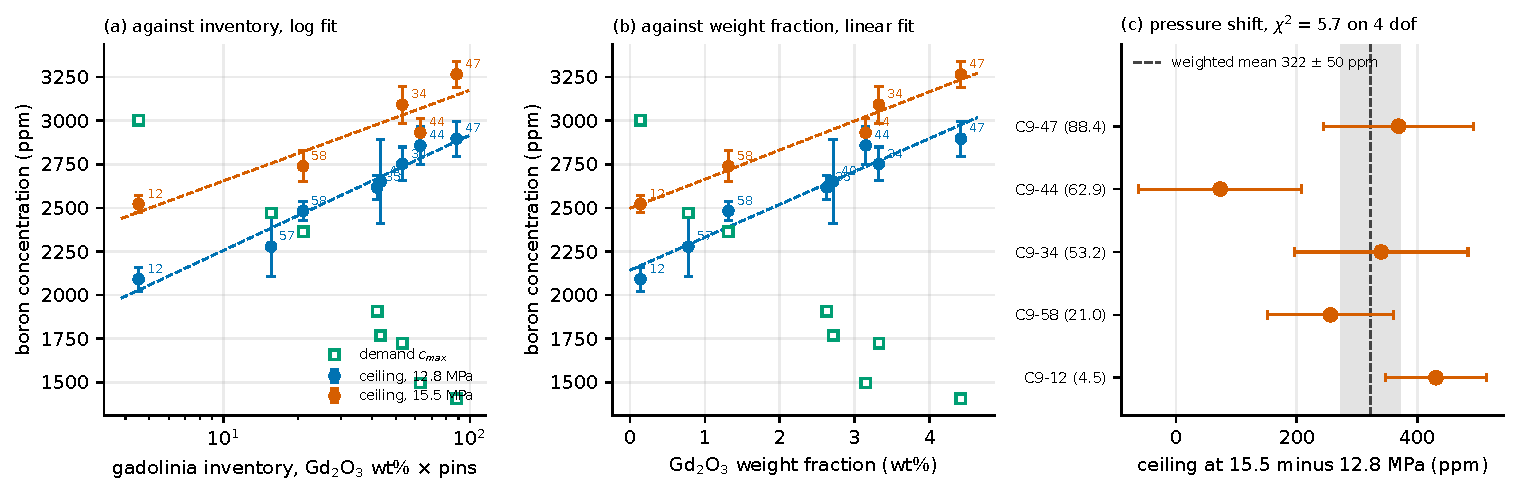
\includegraphics[width=\textwidth]{images/c9_ceiling_two_pressures}
  \caption{Boron ceiling at both pressures against the gadolinia loading.}
  \label{fig:c9-ceiling-2p}
\end{figure}

The ceiling rises with the gadolinia loading at both pressures, and two
measures of that loading were tested:

\begin{itemize}
  \item At \SI{12.8}{MPa} the Spearman coefficient is 1.000 against the
        inventory and 0.976 against the Gd$_2$O$_3$ weight fraction.

  \item At \SI{15.5}{MPa} it is 0.900 against the inventory and 1.000
        against the weight fraction.

  \item The number of gadolinia pins alone shows no correlation at
        either pressure, with coefficients of $-0.07$ and $-0.10$.
\end{itemize}

The two measures rank every lattice identically except C9-34 and C9-44.
Their ceilings differ by \SI{106(146)}{ppm} at \SI{12.8}{MPa}, in favour
of C9-44, and by \SI{161(133)}{ppm} at \SI{15.5}{MPa}, in favour of
C9-34, so this pair is not ordered by either measurement. The present
data therefore do not distinguish the inventory from the weight fraction
as the governing variable.

An unweighted logarithmic fit in the inventory gives the relation below.

\begin{equation}
  c_\mathrm{MTC}(I) = a \ln I + b
  \label{eq:mtc-ceiling-fit}
\end{equation}

\noindent where the symbols have the following meaning:

\begin{itemize}
  \item $c_\mathrm{MTC}$ is the boron concentration at which the
        moderator temperature coefficient crosses zero, in ppm.

  \item $I$ is the gadolinia inventory, the Gd$_2$O$_3$ weight fraction
        in wt\% multiplied by the number of gadolinia pins as built,
        dimensionless.

  \item $a$ is the slope, \SI{287}{ppm} at \SI{12.8}{MPa} and
        \SI{226}{ppm} at \SI{15.5}{MPa}.

  \item $b$ is the intercept, \SI{1595}{ppm} at \SI{12.8}{MPa} and
        \SI{2134}{ppm} at \SI{15.5}{MPa}.
\end{itemize}

The root mean square residual of this fit is \SI{55}{ppm} at
\SI{12.8}{MPa} and \SI{96}{ppm} at \SI{15.5}{MPa}. A straight line in
the weight fraction gives \SI{68}{ppm} and \SI{48}{ppm}. Neither form is
preferred at both pressures.

The pressure shift is consistent with a single value. Over the five
lattices measured twice its weighted mean is \SI{322(50)}{ppm}, with
$\chi^2 = 5.7$ on four degrees of freedom ($p = 0.22$), and no trend
with inventory is resolved.

The verdicts do not depend on the pressure. C9-12 fails its own ceiling
by \SI{912}{ppm} at \SI{12.8}{MPa} and by \SI{481}{ppm} at
\SI{15.5}{MPa}. C9-58 clears by \SI{120}{ppm} and \SI{376}{ppm}, so its
binding pressure is \SI{12.8}{MPa}. The three front designs measured at
both pressures clear by 1027 to \SI{1491}{ppm} at \SI{12.8}{MPa} and by
1367 to \SI{1860}{ppm} at \SI{15.5}{MPa}.

The ceiling and the demand also move in opposite directions with the
same variable. Across the eight lattices at \SI{12.8}{MPa} the ceiling
spans \SI{806}{ppm}, while the operating margin spans \SI{2403}{ppm},
from \SI{-912}{ppm} to \SI{+1491}{ppm}. The demand does most of the work
and the ceiling reinforces it, so a design is either comfortably
operable or clearly not, with little middle ground.

\paragraph{The fidelity of the two sides of the comparison.}
The ceiling is measured on the three-dimensional core model, while the demand is a
two-dimensional core quantity, so the comparison in this section mixes two
fidelities. The rodded confirmation of Section~\ref{sec:res-c9-front}
measures the size of that mismatch. At each design's own critical
concentration the unrodded factor falls from 1.0000 in two dimensions to
0.9704 on the three-dimensional core model, a reactivity difference of 3001 to
\SI{3028}{pcm} across the five front designs, which at their measured boron
worths is 445 to \SI{459}{ppm}.

The three-dimensional demand is therefore about \SI{450}{ppm} below the value
in Table~\ref{tab:c9-front}, and the two-dimensional ceiling is about
\SI{480}{ppm} below the three-dimensional one. Both errors point the same
way, so every margin quoted here is conservative by roughly \SI{900}{ppm}.
The direction of the conclusions is unaffected. The comparison is stated as
it was measured and is not corrected, because a correction would mix a
measured quantity with an inferred one, and a campaign that relied on this
comparison would have to measure both sides on the same model.

\paragraph{Verdicts.}
Of the seven candidates on either peaking front, six clear their own ceiling
and one does not:

\begin{itemize}
  \item C9-47, C9-44, C9-34, C9-40 and C9-35 clear it by 710 to
        \SI{1491}{ppm}, which is 3.7 standard deviations or more. These
        verdicts are not in question.

  \item C9-58 clears by \SI{120}{ppm}, which is 2.3 standard deviations.
        Its ceiling combines two scans, a four-point sweep from 0 to
        \SI{3000}{ppm} and a four-point sweep inside 2200 to
        \SI{2800}{ppm}, which agree with $\chi^2 = 0.86$ on one degree of
        freedom and give \SI{2483}{ppm} together. Further sampling will
        not change the verdict, because the margin itself is the result:
        this design operates at \SI{95}{\%} of what its lattice
        tolerates, against \SI{49}{\%} for C9-47. Its operability is
        therefore not established by this campaign in the sense the other
        five members are.

  \item C9-12 fails it by \SI{912}{ppm}, 13.2 standard deviations. It is the
        one design that entered the front only through the
        three-dimensional peaking of Section~\ref{sec:res-c9-peaking}, and
        it is inoperable whatever its peaking.
\end{itemize}

C9-57, the diagnostic design, fails by \SI{193}{ppm} at 1.1 standard
deviations, and the fidelity mismatch above works in its favour by about
\SI{450}{ppm}, so it would clear on a consistent three-dimensional
comparison. Its verdict is undecided on both counts and is reported as
such. It is not a front candidate and nothing in this chapter depends on
it, but it marks where the combined effect of demand and ceiling places
the boundary, at roughly \SI{1}{wt\%} of gadolinia in this design space.

C9-12 is the only verdict the mismatch cannot overturn. It fails by
\SI{912}{ppm} on the comparison as measured and by roughly \SI{460}{ppm}
once both sides are put on the three-dimensional core model, which is still more than
four standard deviations. The eight lattices also confound the inventory with the
reflector thickness, which is at its bound for seven of the eight, so the
logarithmic law should not be extrapolated outside the converged region of
this campaign.

\subsection{Status of the post-analysis}
\label{sec:res-c9-post}

The post-analysis of Campaign 9 mirrors that of Campaign 8 and is scripted
in \texttt{run\_c9\_post.sh}. The three-dimensional peaking of the front and
of the whole archive with all rods out is reported in
Section~\ref{sec:res-c9-peaking}, the rodded three-dimensional confirmation
of the front in Section~\ref{sec:res-c9-front}, and the boron ceiling of
eight candidate lattices in Section~\ref{sec:res-c9-ceiling}.

The burnup dependence of the Route B k-target leakage factor, which relates
the assembly multiplication factor to the core one and includes the axial
contribution, was measured on the five front designs with the method of
Section~\ref{sec:res-kt-burnup}. Table~\ref{tab:c9-kt-burnup} gives the
result. The two-dimensional to three-dimensional axial factor of
Section~\ref{sec:res-c9-front} is a different quantity and is measured at
beginning of life only.

\begin{table}[htbp]
  \centering
  \small
  \caption{Campaign 9 front: burnup dependence of the Route B leakage factor.}
  \label{tab:c9-kt-burnup}
  \setlength{\tabcolsep}{4.2pt}
  \begin{tabular}{cccccccc}
    \toprule
    Design & $t_\mathrm{refl}$ & $B_\mathrm{EOC}$ & $\mathrm{LF}_\mathrm{BOL}$ &
      $\mathrm{LF}_\mathrm{EOC}$ & $r_\mathrm{EOC}$ & drift &
      $\Delta\mathrm{EFPD}$ \\
    {[--]} & [cm] & [MWd/kgHM] & [--] & [--] & [pcm] & [pcm] & [d] \\
    \midrule
    C9-47 & 5.66 & 19.8 & 1.0823 & 1.0822 & $+15$ & $-17 \pm 194$ & $-2$ \\
    C9-44 & 5.66 & 18.4 & 1.0840 & 1.0830 & $+92$ & $-94 \pm 105$ & $-13$ \\
    C9-34 & 5.66 & 17.8 & 1.0843 & 1.0831 & $+98$ & $-118 \pm 105$ & $-17$ \\
    C9-40 & 5.66 & 18.3 & 1.0823 & 1.0826 & $+51$ & $+23 \pm 109$ & $-6$ \\
    C9-35 & 5.65 & 19.2 & 1.0832 & 1.0824 & $+39$ & $-70 \pm 137$ & $-4$ \\
    \bottomrule
  \end{tabular}
\end{table}

The drifts combine by inverse-variance weighting into a mean of
$-62 \pm 54$\,pcm, with $\chi^2/\nu = 0.26$ over the five designs. The mean is
consistent with zero at 1.2 standard deviations and with the $-13 \pm 30$\,pcm
of the Campaign 8 designs, Equation~\eqref{eq:kt-comp}. The leakage factor
fitted at beginning of life therefore holds to the end of cycle, which is
what justifies the depletion at assembly level.

The residuals behave differently. All five are positive, from $+15$ to
$+98$\,pcm with a mean of $+59$\,pcm, so the measured factor lies above the
tabulated target on every design. Five residuals of the same sign are a
systematic offset in the k-target table and are stated separately from the
drift. The offset is small, about one part in two thousand in the factor,
and it shortens the reported cycle by 2 to 17 days, below one per cent.

C9-34 is the design for which the correction is largest relative to its
margin. Its cycle length of \SI{1841}{d} becomes \SI{1824}{d} once the
end-of-cycle leakage factor is applied, that is \SI{2}{d} below the mission
floor. The correction itself carries an uncertainty of about \SI{15}{d},
propagated from the \SI{105}{pcm} uncertainty of its drift, so the shortfall
is \SI{2+-15}{d} and is not resolved. It is also an order of magnitude
smaller than the \SI{37}{d} uncertainty of the cycle-length proxy at this
mission. The design is therefore retained on the front, with the same caveat
that applies to C9-44, that its compliance with the mission is not
established by this campaign.

Corrections are not applied retroactively to individual designs, because
the front is the set the constraint evaluation produced. A correction
applied to one design and not to the other fifty-nine would not correspond
to any consistent procedure.

The following stages were not complete when this chapter was written:

\begin{enumerate}
  \item The boron ceiling at \SI{15.5}{MPa} on C9-34 and C9-44.

  \item An independent measurement of the boron worth.
\end{enumerate}

\subsection{Limitations}
\label{sec:res-c9-limits}

Six limitations qualify the result of this campaign.

\begin{enumerate}
  \item The reflector is active at its bound. Every front member carries
        the largest reflector the vessel admits, and
        Figure~\ref{fig:c9-design-space} shows that the optimiser reached
        the bound in the first infill iteration and did not test a design
        away from it afterwards. The front is a boundary optimum,
        conditional on the vessel envelope and the clearance of
        Section~\ref{sec:meth-c8-space}.

  \item The cycle-length margin lies inside the proxy uncertainty. The
        front members deliver 1841 to \SI{1947}{d} against a floor of
        \SI{1826}{d}, margins of 15 to 121 days. The core-level validation
        of Section~\ref{sec:res-corevalidation} places the cycle-length
        proxy at about the \SI{2}{\%} level, \SI{37}{d} at this floor, so
        C9-34 and C9-44, at 15 and 32 days, cannot be asserted to meet it.

  \item The boron ceiling is measured at one pressure.
        Section~\ref{sec:res-c9-ceiling} scans eight lattices at
        \SI{12.8}{MPa}, and every candidate on either peaking front except
        C9-12 clears its own ceiling. Only C9-47 is scanned at
        \SI{15.5}{MPa}, and that scan has three points instead of four, so
        it carries no refit uncertainty. The ceiling at the higher pressure
        is therefore known for one design and assumed for the others, and C9-58 clears its own ceiling by only \SI{120}{ppm}, so its
        operability is not established.

  \item Three of the five front members lie inside the noise. Only C9-47
        and C9-34 survive every resample of Table~\ref{tab:c9-stability},
        and the apparent quality of the front is optimistic by \SI{2.8}{\%}
        in hypervolume through selection alone.

  \item The peaking objective is evaluated in two dimensions and at campaign
        fidelity, and a front this narrow is sensitive to both. Raising the
        statistics lowers the hot channel factor by $0.013 \pm 0.004$ on
        the front designs, the three-dimensional model shifts it further by
        an amount that depends on the design, and substituting the
        three-dimensional value changes the non-dominated set in two
        measured ways (Section~\ref{sec:res-c9-peaking}). The front of
        Table~\ref{tab:c9-front} is therefore a set of comparable designs
        and not an ordered ranking.

  \item The depletion runs at a constant \SI{1000}{ppm}, as in every
        campaign, so every cycle length remains a lower bound for a core
        operated with boron letdown, and the critical concentration is
        measured at two states of the cycle only.
\end{enumerate}

Limitations 3 and 5 were the two that could change a conclusion, and both
are now measured. Section~\ref{sec:res-c9-ceiling} gives the ceiling of eight
lattices at \SI{12.8}{MPa} and of C9-47 at both pressures, and
Section~\ref{sec:res-c9-peaking} compares the two- and three-dimensional
peaking over all sixty designs. Neither displaces the selected design, and
the checks that remain are listed in Section~\ref{sec:res-c9-post}.
